\documentclass[oneside]{book}
\usepackage{geometry} % see geometry.pdf on how to lay out the page. There's lots.
\geometry{a4paper, margin = 0.5in} % or letter or a5paper or ... etc
\usepackage{amsmath}
\usepackage{amsfonts}
\usepackage[utf8]{inputenc}
\usepackage[english]{babel}
\usepackage{physics}
\usepackage{amsthm}
\usepackage{amsmath,esint}
\usepackage{paracol}
\renewcommand{\baselinestretch}{1.2}
\usepackage{mathrsfs}
\usepackage{wrapfig}
\usepackage{paracol}
\usepackage{multicol}
\usepackage{graphicx}
\usepackage{subfig}
\usepackage{afterpage}

\newtheorem{theorem}{Theorem}[section]
\theoremstyle{definition}
\newtheorem{definition}{Definition}[section]
\newtheorem{lemma}{Lemma}[section]
\newtheorem{corollary}{Corollary}[section]
\newtheorem{proposition}{Proposition}[section]
\newtheorem{example}{Example}[section]
\newtheorem{problem}{Problem}[section]
\newtheorem{question}{Question}[section]
\newtheorem{remark}{Remark}[section]
\newtheorem{properties}{Properties}[section]
\newtheorem{notation}{Notation}[section]
\newtheorem{axiom}{Axiom}[section]
\newcommand*\B[1]{\mathbf{#1}}
\newcommand*\Bh[1]{\mathbf{\hat{#1}}}
\DeclareMathOperator{\Refl}{Refl}

\makeatletter
\renewcommand*\env@matrix[1][*\c@MaxMatrixCols c]{%
  \hskip -\arraycolsep
  \let\@ifnextchar\new@ifnextchar
  \array{#1}}
\makeatother

\usepackage{mathtools} 

\DeclarePairedDelimiter\ceil{\lceil}{\rceil}
\DeclarePairedDelimiter\floor{\lfloor}{\rfloor}

\title{UML Undergraduate Material}
\author{Ryan Maguire}
\date{\vspace{-5ex}}


\begin{document}
\maketitle
\tableofcontents

\part{Course Work: Mathematics}

\chapter{Calculus I}

\section{CLEP Exam}


\chapter{Linear Algebra}

\section{Miscellaneous Lecture Notes}

\subsection{Orthogonal Projections}

\begin{definition}
If $\{X_1,\hdots, X_k\}$ is a set of $k$ vectors in $\mathbb{R}^n$, then the span of these vectors is the set of all linear combinations. That is, Span$(X_1,\hdots, X_k) = \{\sum_{i=1}^{k} a_i X_i: a_i \in \mathbb{R}\}$
\end{definition}

\begin{remark}
If the vectors $X_1,\hdots, X_k$ are linearly independent, then Span$(X_1,\hdots, X_k)$ is a $k-$dimensional subspace of $\mathbb{R}^n$.
\end{remark}

If we are given a set of $k-$linearly independent vectors in $\mathbb{R}^n$, $\{X_1,\hdots, X_k\}$, and some other vector $Y$, we may wish to consider the orthogonal projection of $Y$ onto the $k-$dimensional subspace spanned the vectors $X_1,\hdots, X_k$. That is, we may wish to find a vector $Y'\in$ Span$(X_1,\hdots, X_k)$ such that $Y-Y'$ is orthogonal to Span$(X_1,\hdots, X_k)$.

\begin{theorem}
If $\{X_1,\hdots, X_k\}$ is a set of $k-$linearly independent vectors in $\mathbb{R}^n$, if $W =$ Span$(X_1,\hdots, X_n)$, and if $Y\in \mathbb{R}^n$ is such that $Y\perp X_i$ for $i=1,2,\hdots, k$, then for all $Z\in W$, $Y\perp Z$.
\end{theorem}
\begin{proof}
For let $Y\in \mathbb{R}^n$ be such that for $i=1,2,\hdots, k$, $Y\perp X_i$. Let $Z\in W$. Then $Z= \sum_{i=1}^{k} a_i X_i$, where $a_i\in \mathbb{R}$. But then $Y\cdot Z = \sum_{i=1}^{k} a_i (Y\cdot X_i) = \sum_{i=1}^{k} a_i 0 = 0$. 
\end{proof}

\begin{lemma}
If $P$ is an $n\times k$ matrix, with $n\leq k$, such that the columns of $P$ are linearly independent, then $P^TP$ is invertible.
\end{lemma}
\begin{proof}
Suppose $P^TPX = 0$. Then $PX$ is orthogonal to the columns of $P$. But $PX$ is a linear combination of the columns of $P$, and thus $PX$ must be orthogonal to itself. Therefore $PX = 0$. But as the columns of $P$ are linearly independent, if $PX = 0$, then $X=0$. Thus $P^TPX = 0$ if and only if $X=0$. Thus $P^TP$ is invertible.
\end{proof}

So we need $X_i^T(Y-Y') = 0$ for $i=1,2,\hdots, k$. Let $X_i = (x_{1i},x_{2i},\hdots, x_{ni})$ and let $P = \begin{bmatrix} x_{11} & x_{12} & \hdots & x_{k1} \\ x_{21} & x_{22} & \hdots & x_{k2} \\ \vdots & \vdots & \ddots & \vdots \\ x_{n1} & x_{n2} & \hdots & x_{nk}\end{bmatrix}$. Then we have $P^T(Y-Y') = 0$, or $P^TY = P^T Y'$. But $Y'\in W$, so $Y' = \sum_{i=1}^{k} c_i X_i = P(c_1,\hdots, c_k)^T = PC$. So we have $P^TY = P^TPC$, and thus $C = (P^TP)^{-1}P^TY$. Thus $Y'=P(P^TP)^{-1}P^T Y$.

\begin{definition}
The matrix $P(P^TP)^{-1}P^T$ is called the projection matrix of $W$.
\end{definition}

\begin{theorem}
If $Q = P(P^TP)^{-1}P^T$ is a projection matrix for some subspace $W$, then the following are true:
\begin{enumerate}
\item $Q^T =Q$.
\item $Q^2 = Q$.
\end{enumerate}
\end{theorem}
\begin{proof}
In order,
\begin{enumerate}
\item $Q^T = \big(P(P^TP)^{-1}P^T\big)^T = (P^T)^T\big(P(P^TP)^{-1}\big)^T = P \big((P^TP)^{-1}\big)^TP^T = P((P^TP)^T)^{-1}P^T = P(P^TP)^{-1}P^T=Q$.
\item $Q^2 = QQ = P(P^TP)^{-1}P^T P(P^TP)^{-1}P^T = P\big((PT^TP)^{-1}(P^TP)\big)(P^TP)^{-1}P^T = P(P^TP)^{-1}P^T = Q$. Let $Y\in \mathbb{R}^n$ be arbitrary. 
\end{enumerate}
\end{proof}

\begin{theorem}
The matrix $Q$ is a projection matrix for the subspace $W$ if and only if $Q^T=Q^2=Q$.
\end{theorem}

\subsection{Reflections}

Let $W$ be a plane passing through the origin, and suppose we want to reflect a vector $v$ across this plane. Let $u$ be a unit vector along $W^{\perp}$. That is, $u$ is normal to the plane. The projection of $v$ along the line through $u$ is then given by: $\hat{v} = Proj_{u}(v) = u(u^Tu)^{-1}u^Tv$. But as $u$ is a unit vector, $u^Tu = 1$, so $\hat{v} = uu^T v$. Let $Q_u = uu^T$. The definition of the reflection of $v$ across $W$ is the vector $\Refl_{W}(v)$ such that has the same magnitude as $v$ lying on the opposite side of $W$. Thus $v-\Refl_{W}(v) = 2Q_u v$, so $\Refl_{W}(v)= v-2Q_u v = (I-2Q_u)v =(I-2uu^T)v$. 

\begin{definition}
$H_W = I-2uu^T$ is called the reflection matrix for the plane $W$. It is also called the Householder matrix.
\end{definition}

\begin{definition}
A matrix $P$ is orthogonal if $P^TP = I$.
\end{definition}

\subsection{Lecture Notes on Orthogonal Matrices}

\begin{definition}
An $n\times n$ real-valued matrix $A$ is said to be an orthogonal matrix if $A^TA = I$.
\end{definition}

\begin{theorem}
If $A$ is an orthogonal matrix, then $A^T = A^{-1}$.
\end{theorem}
\begin{proof}
For $A^TA = I$, and inverses are unique. Thus $A^T = A^{-1}$.
\end{proof}

If we let $A_{i} = Ae_{i}$, then $A^TA = \begin{bmatrix} A_1^TA_1 & \hdots & A_1^TA_n \\ \vdots & \ddots & \vdots \\ A_n^TA_1 & \hdots & A_n^TA_n\end{bmatrix} = I$. Therefore $A_i^TA_j = \begin{cases} 1, & i=j \\ 0, & i\ne j\end{cases}$.

\begin{theorem}
If $A$ is an $n\times n$ real-valued matrix and $A_i = Ae_i$, $i=1,2,\hdots, n$, then $A$ is orthogonal if and only if $\{A_1,\hdots, A_n\}$ is an orthonormal set of vectors.
\end{theorem}
\begin{proof}
If $A$ is orthogonal, then $A_i^TA_j = \begin{cases} 1, & i=j \\ 0, & i\ne j\end{cases}$, and from this we have orthonormality. If $\{A_1,\hdots, A_n\}$ is orthonormal, then $A^TA = I$ and is therefore orthogonal.
\end{proof}

\begin{theorem}
The following statements are equivalent:
\begin{enumerate}
\item $A$ is an orthogonal matrix.
\item $|AX| = |X|$ for all $X\in \mathbb{R}^n$.
\item $AX\cdot AY = X\cdot Y$ for all $X,Y\in \mathbb{R}^n$.
\end{enumerate}
\end{theorem}
\begin{proof}
We show $1\Rightarrow 2 \Rightarrow 3 \Rightarrow 1$.
\begin{enumerate}
\item If $A$ is orthogonal, then $A^TA = I$. But then $|AX|^2 = (AX)^TAX = X^TA^TAX = X^TIX = X^TX = |X|^2$. Therefore $|AX| = |X|$.
\item If $A$ is a square matrix such that $|AX| = |X|$ for all $X\in \mathbb{R}^n$, then $|X+Y|^2 = (X+Y)^T(X+Y) = X^TX+X^TY+Y^TX+Y^TY = |X|^2+2X^TY+|Y|^2$. But $|A(X+Y)|^2 = |AX+AY|^2 = |AX|^2+2(AX)^TAY+|AY|^2 = |X|^2+2(AX)^TAY+|Y|^2$. Therefore $(AX)^TAY = X^TY$. That is, $AX\cdot AY = X\cdot Y$.
\item If $A$ is a square matrix such that $AX\cdot AY = X\cdot Y$ for all $X,Y\in \mathbb{R}^n$, and if $A_i =  Ae_i$, then $A_i^TA_j = (Ae_i)^TAe_j = Ae_i \cdot Ae_j = e_i \cdot e_j = \begin{cases} 1, & i = j \\0, & i\ne j\end{cases}$. Therefore, $A$ is orthogonal.
\end{enumerate}
\end{proof}

\begin{theorem}
If $A$ and $B$ are $n\times n$ orthogonal matrices, then $AB$ is orthogonal.
\end{theorem}
\begin{proof}
For if $A^TA = I$ and $B^TB = I$, then $(AB)^TAB = B^TA^TAB = B^TIB = B^TB = I$. Therefore $AB$ is orthogonal.
\end{proof}

\begin{theorem}
If $A$ is an $n\times n$ orthogonal matrix, then $\det(A) = 1$ or $-1$.
\end{theorem}
\begin{proof}
For $1 = \det(I) = \det(A^TA) = \det(A^T)\det(A) = \det(A)^2$. Therefore $\det(A) = \pm 1$.
\end{proof}

\begin{remark}
The converse is false. There exist matrices with determinants $\pm 1$ that are not orthogonal.
\end{remark}

Recall that if $u\in \mathbb{R}^n$ is a unit vector and $W = u^{\perp}$, then $H = I=2uu^T$ is the reflection matrix for the subspace $W$. Reflections preserve distance, and therefore $H$ must be an orthogonal matrix. 

\begin{theorem} If $A$ is an $n\times n$ orthogonal matrix, then there exist $k$ $n\times n$ reflection matrices $H_1,\hdots, H_k$, $0\leq k \leq n$, such that $A = \prod_{i=1}^{j}H_i$.
\end{theorem}
\begin{proof}
We prove by induction. The base case is trivial. Suppose it holds for $n-1$. Let $z = Ae_n$, and let $H$ be the reflection matrix that exchanges $z$ and $e_n$. Then $HAe_n = Hz = e_n$, so $HA$ fixes $e_n$. But $HA$ is an orthogonal matrix, and thus preserves distances and angles. Thus $HA$ maps $\mathbb{R}^{n-1}$ onto itself, and thus by induction there are $H_2,\hdots, H_k$ such that $HA = \prod_{i=2}^{k} H_i$. Letting $H=H_1$, we have $A = HHA = \prod_{i=1}^{k}H_i$. Therefore, etc.
\end{proof}

\begin{theorem}
If $H$ is a reflection matrix, then $\det(H) = -1$.
\end{theorem}

\begin{theorem}
If $A$ is an orthogonal matrix and $A=\prod_{i=1}^{k} H_i$, then $\det(A) = (-1)^k$.
\end{theorem}

If $A$ is an orthogonal $2\times 2$ matrix, then we know that columns must be unit vectors that are also orthogonal (Orthonormal). That is, the two columns must lie on the unit circle about the origin. So we may express the first column as $\big(\cos(\theta),\sin(\theta)\big)$ for some angle $\theta$. There are then two options for the seconds column: $\big(-\sin(\theta),\cos(\theta)\big)$ or $\big(\sin(\theta),-\cos(\theta)\big)$. The first is the rotation matrix which rotates $\mathbb{R}^2$ counterclockwise around the origin, and the second is the reflection matrix that makes a reflection across the line that makes an angle $\frac{\theta}{2}$ with the $x-$axis. 

\begin{theorem}
If $A$ is a $3\times 3$ orthogonal matrix, then one of the following is true:
\begin{enumerate}
\item If $\det(A) = 1$, then $A$ is a rotation matrix.
\item If $\det(A) = -1$ and $A=A^T$, then either $A=-I$ or $A$ is a reflection matrix.
\item If $\det(A) = -1$ and $A\ne A^T$, then $A$ is the product of three reflections.
\end{enumerate}
\end{theorem}
\begin{proof}
$A$ must be the product of $0,1,2,$ or $3$ reflection matrices. If $\det(A) = 1$, then $A$ is the product of an even number of reflections, and thus either $A=I$ or $A$ is the product of two reflections, and is thus a rotation. If $\det(A)=-1$, then $A$ is the product of an odd number of reflections, either $1$ or $3$. If $A$ is a single reflection, then $A=H$ for some Householder matrix $H$. Thus $A^T = A$. Conversely, if $A = A^T$ and $\det(A) = -1$, then $\det(-A) = 1$, and $-A^T = -A = -A^{-1}$. Therefore $-A$ is a rotation whose square is the identity. If $A\ne I$, then $A$ must be a rotation of $\pi/2$ around some axis, and thus $A$ is a reflection. If $\det(A) = -1$, and $A\ne A^T$, then $A$ cannot be a rotation or a pure reflection, and thus $A$ is the product of $3$ reflection matrices.
\end{proof}

\begin{theorem}
If $A$ and $B$ are $3\times 3$ rotation matrices, then $A\times B$ is a rotation matrix.
\end{theorem}
\begin{proof}
For $A$ and $B$ must be orthogonal, and thus $AB$ is orthogonal. But $\det(AB) = \det(A)\det(B) = 1\cdot 1 = 1$, and thus $AB$ is an orthogonal matrix with determinant equal to $1$, and is thus a rotation matrix.
\end{proof}

\subsection{Rotations}

The $2\times 2$ matrix $A_{\theta} = \begin{bmatrix} \cos(\theta) & -\sin(\theta) \\ \sin(\theta) & \cos(\theta)\end{bmatrix}$ rotates the plane $\mathbb{R}^2$ counter-clockwise by the angle $\theta$ around the origin. The question that then arise is, "Is there a similar way to do this for $\mathbb{R}^3$? The simple case would be rotating by an angle $\theta$ about the $z-$axis, analogous the rotating the Earth by $\theta$ about the North Pole. This fixes the $z-$axis and acts on the $xy-$plane only. This can be represented by the matrix $S_{\theta} = \begin{bmatrix} \cos(\theta) & -\sin(\theta) & 0 \\ \sin(\theta) & \cos(\theta) & 0 \\ 0 & 0 & 1 \end{bmatrix}$. $S_{\theta}$ is an orthogonal matrix. That is, $S_{\theta} S_{\theta}^T = I$, and therefore $S_{\theta}^T = S_{\theta}^{-1}$. Suppose we want to rotate by an angle $\theta$ about a different axis. Let $\B{u}$ be a unit vector pointing in the direction of the axis of rotation and let $R_{\theta,\B{u}}$ be the new rotation matrix. To compute $R_{\theta,\B{u}}$ we need to choose a unit vector $\B{v}$ that is orthogonal to $\B{u}$. Let $\B{w} = \B{u}\times \B{v}$. Then $\{\B{u},\B{v},\B{w}\}$ is an orthonormal basis of $\mathbb{R}^3$ such that $\B{v}\times \B{w} = \B{u}$. Let $P = \begin{bmatrix} v_1 & w_1 & u_1 \\ v_2 & w_2 & u_2 \\ v_3 & w_3 & u_3 \end{bmatrix}$. The columns of $P$ form an orthonormal set, and therefore $P$ is orthogonal. In particular, $P^T\B{u} = \begin{bmatrix} v_1 & v_2 & v_3 \\ w_1 & w_2 & w_3 \\ u_1 & u_2 & u_3 \end{bmatrix}\B{u} = \begin{bmatrix} \B{v}\cdot \B{u} \\ \B{w} \cdot \B{u} \\ \B{u} \cdot \B{u}\end{bmatrix} = \begin{bmatrix} 0 \\ 0 \\ 1 \end{bmatrix}$. Similarly, $P^T \B{u} = \begin{bmatrix} 1 \\ 0 \\ 0 \end{bmatrix}$ and $P^T \B{w} = \begin{bmatrix} 0 \\ 1 \\ 0 \end{bmatrix}$.

\begin{theorem}
If $\theta \in [0,2\pi]$ and $\B{u}\in \mathbb{R}^3$ is a unit vector, then $R_{\theta, \B{u}} = PS_{\theta}P^T$.
\end{theorem}
\begin{proof}
$PS_{\theta}P^T$ fixes $\B{u}$, for $PS_{\theta}P^T\B{u} = PS_{\theta} \begin{bmatrix}0 & 0 & 1 \end{bmatrix} = P\begin{bmatrix} 0 & 0 & 1 \end{bmatrix} = \B{u}$. $PS_{\theta}P^T\B{v} = \cos(\theta)\B{v}+\sin(\theta) \B{w}$ and $PS_{\theta}P^T \B{w} = -\sin(\theta) \B{v}+\cos(\theta) \B{w}$. More general, if $X = a\B{v}+b\B{w}+c\B{u}$, then $PS_{\theta}P^TX = a(\cos(\theta)\B{v}+\sin(\theta)\B{w})+b(-\sin(\theta) \B{v}+\cos(\theta)\B{w})+c\B{u} = R_{\theta,\B{u}}X$.
\end{proof}

From the orthogonality of $P$ and $S_{\theta}$ we have that $R_{\theta,\B{u}}$ is also orthogonal.

\begin{theorem}
A rotation matrix $R$ is an orthogonal matrix with determinant $1$.
\end{theorem}
\begin{proof}
For $R^TR = (PS_{\theta}P^T)^TPS_{\theta}P^T = PS_{\theta}^TP^TPS_{\theta}P^T = PS_{\theta}^TS_{\theta}P^T = PP^T = I$. Also $\det(R) = \det(PS_{\theta}P^T) = \det(P)\det(S_{\theta})\det(P^T) = \det(P)\det(S_{\theta})\det(P^{-1}) = \det(P)\det(S_{\theta})\frac{1}{\det(P)} = \det(S_{\theta}) = 1$.
\end{proof}

\begin{remark}
The converse of the previous theorem is also true. A matrix $R$ is a rotation matrix if and only if it is orthogonal and has determinant $1$.
\end{remark}

We now turn to the question of how to compute the rotation of $\mathbb{R}^3$ represented by a given orthogonal matrix. If $R$ is an orthogonal matrix such that $\det(R) = 1$, how do we compute the angle of rotation? Firstly, recall that the trace of a matrix $\Tr(A)$, is the sum of the diagonal components $\Tr(A) = a_{11}+\hdots + a_{nn}$.

\begin{theorem}
If $R$ is a rotation matrix of angle $\theta$, then $\cos(\theta) = \frac{\Tr(R) - 1}{2}$.
\end{theorem}
\begin{proof}
Recall that if $A$ is a square $n\times n$ matrix and $P$ is an $n\times n$ invertible matrix, then $\Tr(PAP^{-1}) = \Tr(A)$. This is because for any two $n\times n$ matrices $A$ and $B$, $\Tr(AB) = \Tr(BA)$. But $R = PS_{\theta} P^T = PS_{\theta}P^{-1}$, and so $\Tr(R) = \Tr(PS_{\theta}P^{-1}) = \Tr(S_{\theta}) = 1+2\cos(\theta)$. Therefore $\cos(\theta) = \frac{\Tr(R)-1}{2}$.
\end{proof}

This doesn't tell us everything, as we still don't know $\B{u}$, and $\cos(\theta) = \cos(-\theta)$, so we still don't know the sign of $\theta$. Since $R$ is an orthogonal matrix, $R^T = R^{-1}$. So if $\B{u}$ lies on the axis of rotation, then $(R-R^T)\B{u} = R\B{u}-R^{-1}\B{u} = \B{u}-\B{u} = 0$. Thus we can find the axis of rotation by determining the null space of $R-R^T$. Let $R = \begin{bmatrix} r_{11} & r_{12} & r_{13} \\ r_{21} & r_{22} & r_{23} \\ r_{31} & r_{32} & r_{33} \end{bmatrix}$. Then $R-R^T = \begin{bmatrix} 0 & r_{12} - r_{21} & r_{13} - r_{31} \\ r_{21} - r_{12} & 0 & r_{23}-r_{32} \\ r_{31} - r_{13} & r_{32} - r_{23} & 0 \end{bmatrix}$. Let $\alpha = r_{12} - r_{21},\beta = r_{13} - r_{31},$ and $\gamma = r_{23}-r_{32}$. Then $R-R^T = \begin{bmatrix} 0 & \alpha & \beta \\ -\alpha & 0 & \gamma \\ -\beta & -\gamma & 0 \end{bmatrix}$. This suggests that $\B{u}$ is parallel to $\begin{bmatrix} -\gamma \\ \beta \\ -\alpha \end{bmatrix} = \begin{bmatrix} r_{32}-r_{23} \\ r_{13}-r_{31} \\ r_{21}-r_{12} \end{bmatrix}$.

\begin{theorem}
If $R$ is a rotation matrix such that $R\ne R^T$, then the axis of rotation of $R$ is parallel to $\B{q}=\begin{bmatrix}-\gamma \\ \beta \\ -\alpha\end{bmatrix}$. Indeed, if $\B{u}$ is a unit vector about the axis of rotation, then $\B{q} = 2\sin(\theta)\B{u}$.
\end{theorem}
\begin{proof}
Let $R = PS_{\theta}P^T$. Then $R-R^T = PS_{\theta}P^T - PS_{\theta}^TP^T = P(S_{\theta}-S_{\theta}^T)P^T = P\begin{bmatrix}0 & -2\sin(\theta) & 0 \\ 2\sin(\theta) & 0 & 0 \\ 0 & 0 & 0 \end{bmatrix}P^T = 2\sin(\theta)(\B{w}\cdot \B{w}\B{v}^T - \B{v}\B{w}^T)$, where $\B{v}$ is a chosen vector orthogonal to $\B{u}$ and $\B{w} = \B{u}\times \B{v}$. Therefore $\begin{bmatrix} -\gamma \\ \beta \\ -\alpha \end{bmatrix} = 2\sin(\theta) \B{v}\times \B{w} = 2\sin(\theta) \B{u}$.
\end{proof}

\begin{remark}
What about the case when $R-R^T = 0$? When this happens either $\theta = 0$ or $\theta = \pi$. If $\theta = 0$, then this is the identity rotation and thus $R = I$, and we are done. If $R\ne I$, then $\theta = \pi$. To find out the axis of rotation, we have that $R = PS_{\pi}P^T = \begin{bmatrix}-1 & 0 & 0 \\ 0 & -1 & 0 \\ 0 & 0 & 1 \end{bmatrix} = -\B{v}\B{v}^T - \B{w}\B{w}^T +\B{u}\B{u}^T$. But $\B{v},\B{w},$ and $\B{u}$ form an orthonormal basis, and therefore $\B{v}\B{v}^T + \B{w}\B{w}^T+\B{u}\B{u}^T = I$. Therefore $R = -I+2\B{u}\B{u}^T$, so $\B{u} \B{u}^T = \frac{1}{2}(R+I)$. But the columns of $\B{u}\B{u}^T$ are parallel to $\B{u}$, and therefore we can determine $\B{u}$ by normalizing one of the columns of $\frac{1}{2}(R+I)$.
\end{remark}

\subsection{The Matrix Exponential}

\begin{definition}
If $A$ is an $n\times n$ matrix, then the matrix exponential of $A$ is $e^{A} =\sum_{k=0}^{\infty} \frac{A^k}{k!}$.
\end{definition}

\begin{remark}
Notationally, we write $A^0 = I$. For any complex-valued matrix $A$ of finite dimension, it can be shown that this sum converges.
\end{remark}

\begin{theorem}
If $A$ and $P$ are complex $n\times n$ matrices and $P$ is invertible, then $e^{P^{-1}AP} = P^{-1}e^{A}P$.
\end{theorem}
\begin{proof}
For all $m\in \mathbb{N}$, $(P^{-1}AP)^m = P^{-1}A^mP$. Thus $e^{P^{-1}AP} = \sum_{k=0}^{\infty} P^{-1}\frac{A^k}{k!}P = P^{-1}\big(\sum_{k=0}^{\infty} \frac{A^k}{k!}\big)P = P^{-1}e^A P$.
\end{proof}

\begin{theorem}
If $0$ is the zero matrix, then $e^0 = I$.
\end{theorem}

\begin{theorem}
If $A$ is an $n\times n$ matrix and $m\in \mathbb{N}$, then $A^m e^A = e^A A^m$.
\end{theorem}
\begin{proof}
For $A^m e^A = A^m \sum_{k=0}^{\infty} \frac{A^k}{k!} = \sum_{k=0}^{\infty} \frac{A^{k+m}}{k!} = \big(\sum_{k=0}^{\infty} \frac{A^k}{k!}\big)A^m$.
\end{proof}

\begin{theorem}
If $A$ is an $n\times n$ matrix, then $e^{A^T} = (e^A)^T$.
\end{theorem}
\begin{proof}
For $e^{A^T} = \sum_{k=0}^{\infty} \frac{(A^T)^k}{k!} = \sum_{k=0}^{\infty} \frac{(A^k)^T}{k!} = \big(\sum_{k=0}^{\infty} \frac{A^k}{k!}\big)^T = (e^A)^T$.
\end{proof}

\begin{theorem}
If $A$ and $B$ are $n\times n$ matrices and if $AB = BA$, then $Ae^B = e^B A$.
\end{theorem}
\begin{proof}
For $Ae^B = A\sum_{k=0}^{\infty} \frac{B^k}{k!} = \sum_{k=0}^{\infty} A\frac{B^k}{k!} = \sum_{k=0}^{\infty} \frac{B^k}{k!}A = \big(\sum_{k=0}^{\infty} \frac{B^k}{k!}\big)A = e^BA$.
\end{proof}

\begin{theorem}
If $A$ and $B$ are $n\times n$ matrices and $AB = BA$, then $e^{A}e^{B} = e^{B}e^{A}$.
\end{theorem}
\begin{proof}
For $e^A e^B = e^A\sum_{k=0}^{\infty} \frac{B^k}{k!} = \sum_{k=0}^{\infty} e^A\frac{B^k}{k!} = \sum_{k=0}^{\infty} \big(\sum_{j=0}^{\infty} \frac{A^j}{j!}\big) \frac{B^k}{k!} = \sum_{k=0}^{\infty}\big(\sum_{j=0}^{\infty} \frac{A^j}{j!}\frac{B^k}{k!}\big) = \sum_{k=0}^{\infty}\big(\sum_{j=0}^{\infty} \frac{B^k}{k!}\frac{A^j}{j!}\big) = \sum_{k=0}^{\infty} \frac{B^k}{k!} \sum_{j=0}^{\infty} \frac{A^j}{j!} = e^Be^A$.
\end{proof}

If is NOT true that $e^{A+B} = e^Ae^B$, in general. Matrix exponentiation lacks this feature. The following is true:

\begin{theorem}
If $A$ is a $n\times n$ matrix and $s,t\in \mathbb{C}$, then $e^{A(s+T)} = e^{As}e^{At}$.
\end{theorem}
\begin{proof}
For $e^{As}e^{At} = \sum_{j=0}^{\infty} \sum_{k=0}^{\infty} \frac{A^{j+k}s^jt^k}{j!k!}$. Letting $n = j+k$, so $j = n-k$, we have $\sum_{n=0}^{\infty} \sum_{k=0}^{\infty} \frac{A^n}{n!}\frac{n!}{k!(n-k)!}s^{n-k}t^k = \sum_{n=0}^{\infty}\frac{A^n}{n!}\big(\sum_{k=0}^{\infty} \frac{n!}{k!(n-k)!}s^{n-k}t^k\big)$. From the binomial theorem, the expression inside the parenthesis is equal to $(s+t)^n$. So we have $e^{As}e^{At}=\sum_{n=0}^{\infty} \frac{A^n(t+s)^n}{n!} = e^{A(s+t)}$.
\end{proof}

\begin{theorem}
If $A$ is an $n\times n$ matrix, then $e^A$ is invertible and $(e^A)^{-1} = e^{-A}$.
\end{theorem}
\begin{proof}
For $I = e^{0} = e^{A(1-1)} = e^Ae^{-A}$. Thus $(e^{A})^{-1} = e^{-A}$.
\end{proof}

\begin{theorem}
If $A$ is an $n\times n$ matrix and $t\in \mathbb{R}$, then $\frac{d}{dt}\big(e^{At}\big) = Ae^{At}$.
\end{theorem}
\begin{proof}
For $\underset{h\rightarrow 0}\lim \frac{e^{A(t+h)}-e^{At}}{h} = e^{At}\underset{h\rightarrow 0}\lim \frac{e^{Ah}-I}{h} = e^{At}\underset{h\rightarrow 0}\lim\big[A+\frac{A^2}{2!}h+\hdots\big] = e^{At}A = Ae^{At}$.
\end{proof}

\begin{theorem}
If $A$ and $B$ are $n\times n$ matrices and $AB=BA$, then $e^{A+B} = e^Ae^B$.
\end{theorem}
\begin{proof}
For let $g(t) = e^{(A+B)t}e^{-Bt}e^{-At}$. Then from commutativity of $A$ and $B$, $g'(t) = 0$. But then $g(t)$ is a constant. From the definition, $g(0) = I$, and thus $g(t) = I$. So $e^{(A+B)t}e^{-Bt}e^{-At} = I$, and therefore $e^{(A+B)t} = e^{At}e^{Bt}$.
\end{proof}

\begin{theorem}
If $A^2 = 0$, then $e^A = I+A$.
\end{theorem}
\begin{proof}
For $e^A = I+A+A^2\big(\frac{I}{2!}+\frac{A}{3!}+\hdots\big) = I+A+0 = I+A$.
\end{proof}

\subsection{Linear Systems of Ordinary Differential Equations}

Consider the equation $y' = ky$, where $k$ is some constant. We can solve this via calculus using separation of variables: $\frac{y'}{y} = k\Rightarrow \int \frac{y'}{y}dx = \int kdx \Rightarrow \ln(y) = kx+c \Rightarrow y = e^c e^{kx}$. Setting $x=0$, we have $e^c = y_0$. So $y = y_0e^{kx}$. Let us solve this a different way: Let $F(x) = e^{-kx}y$, and let $y'=kx$. Differentiating we have $F'(x) = -ke^{kx}y + e^{-kx}y' = -ke^{-kx}+e^{=kx}ky = 0$. So $F'(x) = 0$, and therefore $F(x)$ is a constant. Setting $x=0$, we have $F(x) = y_0$. So $y = y_0e^{kx}$. This shows us that $y_0e^{kx}$ is the $only$ solution to this problem. Let $Y(t) = \begin{bmatrix} y_1(t) \\ y_2(t)\end{bmatrix}$. Let $A=\begin{bmatrix} 5 & 1 \\ -2 & 2 \end{bmatrix}$ and consider the system $Y'(t) = AY(t)$. Let $F(t) = e^{-At}Y(t)$. Then $F'(t) = 0$, and we have that $Y(t) = Y_0 e^{At}$.

\begin{theorem}
If $Y:\mathbb{R}\rightarrow \mathbb{R}^n$ is a differentiable function such that $Y'(t) = AY(t)$, where $A$ is a diagonalizable matrix with eigenvalues $\lambda_1,\hdots, \lambda_n$ and eigenvectors $v_1,\hdots, v_n$, then $Y(t) = \sum_{k=1}^{n} \lambda_k e^{\lambda_k t}v_k$
\end{theorem}


\section{Problem Sets}

\subsection*{Problem Set I}

\begin{problem}
Find the point on the line $y=4x$ which is closest to the point $(2,5)$.
\end{problem}
\begin{proof}[Solution 1]
Given a vector $\B{v}$ that is parallel to the line $y$, we know that the vector $\B{w}$ from $(2,5)$ to the point $(x,y)$ that minimizes the distance from $y=4x$ to the point $(2,5)$ will satisfy $\B{v}\cdot \B{w} = 0$. That is, $(1,4)\cdot (2-x,5-y) = 0\Rightarrow 2-x+4(5-y) = 0 \Rightarrow 22 - x - 4 y = 0$. As $y = 4x$, this reduces to $22-17x = 0 \Rightarrow x= \frac{22}{17}$. Thus the point of least distance is $\frac{22}{17}(1,4)$.
\end{proof}
\begin{proof}[Solution 2]
This point is the projection of the vector $(2,5)^T$ onto $(1,4)^T$. That is, $\B{P} = \frac{\begin{bmatrix}2 & 5 \end{bmatrix} \begin{bmatrix} 1 \\ 4 \end{bmatrix}}{\begin{bmatrix} 1 & 4 \end{bmatrix} \begin{bmatrix} 1 \\ 4 \end{bmatrix}} \begin{bmatrix} 1 \\ 4 \end{bmatrix} = \frac{22}{17} \begin{bmatrix} 1 \\ 4\end{bmatrix}$
\end{proof}

\begin{problem}
Show that $\B{x}\B{y}^T + \B{y}\B{x}^T$ is symmetric.
\end{problem}
\begin{proof}[Solution]
Recall that a matrix is symmetric if it is equal to its transpose. Thus, we must show $A = A^T$. But for any $n\times n$ matrices $A$ and $B$, $(A+B)^T = A^T + B^T$, and $(AB)^T = B^T A^T$, and $(A^T)^T = A$. Thus, given our matrix $A= \B{x}\B{y}^T + \B{y}\B{x}^T$, we have that $A^T = (\B{x}\B{y}^T + \B{y}\B{x}^T)^T = (\B{x}\B{y}^T)^T + (\B{y}\B{x}^T)^T = (\B{y}^T)^T\B{x}^T + (\B{x}^T)^T\B{y}^T = \B{y}\B{x}^T + \B{x}\B{y}^T = \B{x}\B{y}^T + \B{y}\B{x}^T = A$
\end{proof}

\begin{problem}
Compute the product $\begin{bmatrix} 2 & -1 \\ 3 & 1\end{bmatrix} \begin{bmatrix} -1 & 2 & 3 & 1 \\ 2 & -2 & 1 & -1 \end{bmatrix}$
\end{problem}
\begin{proof}[Solution]
$\begin{bmatrix} 2 & -1 \\ 3 & 1\end{bmatrix} \begin{bmatrix} -1 & 2 & 3 & 1 \\ 2 & -2 & 1 & -1 \end{bmatrix}=\begin{bmatrix} 2(-1)+(-1)2 & 2\cdot 2 + (-1)(-2) & 2\cdot 3 + (-1)1 & 2\cdot 1 + (-1)(-1) \\ 3(-1)+1\cdot 2 & 3\cdot 2 + 1(-2) & 3\cdot 3 + 1\cdot 1 & 3\cdot 1 + 1(-1)\end{bmatrix}\\ =\begin{bmatrix} -4 & 6 & 5 &3 \\ -1 & 4 & 10 & 2\end{bmatrix}$
\end{proof}

\begin{problem}
Find the equation of the plane that passes through the points $P_1(2,2,1),\ P_2(2,3,2),\ P_3(-1,3,1)$.
\end{problem}
\begin{proof}[Solution]
It suffices to find a vector normal to this plane. Let $\overrightarrow{P_1P_2} = \begin{bmatrix} 2-2 \\ 3-2 \\ 2-1 \end{bmatrix} = (0,1,1)^T$ be the relative position vector from $P_1$ to $P_2$, and similarly define $\overrightarrow{P_1P_3} = \begin{bmatrix} -1-2 \\ 3-2 \\ 1-1 \end{bmatrix} = (-3,1,0)^T$. Then both vectors are parallel to the plane, and thus $\overrightarrow{P_1P_2}\times \overrightarrow{P_1P_3}=(-1,3,3)^T$ is perpendicular to the plane. Suppose $Q=(x,y,z)$ is a point in the plane. Then the relative position vector $P_1 Q = (x-2,y-2,z-1)^T$ is orthogonal to $(-1,3,3)^T$. Thus $(x-2,y-2,z-1)(-1,3,3)^T = 0$, so $2-x+3y-6+3z-3 = 0 \Rightarrow x-3y-3z +7 = 0$. As $(x,y,z)$ is an arbitrary point in the plane, this is the equation of the plane.
\end{proof}

\begin{problem}
Let $S$ be the subspace of $\mathbb{R}^3$ spanned by $\B{x}_1 = (1,-1,2)^T$ and $\B{x}_2 = (-1,2,2)^T$. Find a basis for $S^{\perp}$
\end{problem}
\begin{proof}[Solution]
We seek a vector in $\B{x}_3\in\mathbb{R}^3$ such that $\B{x}_3\cdot \B{x}_{1,2} = 0$. Or in other words, $\begin{bmatrix} 1 & -1 & 2 \\ 0 & 1 & 4 \end{bmatrix} \begin{bmatrix} x_1 \\ x_2 \\ x_3 \end{bmatrix} = 0$. This gives the following:
\begin{eqnarray}
x_1 - x_2 + 2x_3 &&= 0\\
	x_2 + 4x_3 &&= 0
\end{eqnarray}
This gives us $x_2 = -4x_3$, so $x_1 + 6x_3 = 0$, or $x_1=-6x_3$. Thus $\B{x}_3 = x_3(-6,-4,1)^T$. $x_3$ is a free variable.
\end{proof}

\begin{problem}
For the matrix $A = \begin{bmatrix} 1 & 2 & 2 \\ -1 & -1 & 0 \end{bmatrix}$, find a basis for the following:
\begin{enumerate}
\begin{multicols}{4}
\item $R(A^T)$
\item $N(A)$
\item $R(A)$
\item $N(A^T)$
\end{multicols}
\end{enumerate}
\end{problem}
\begin{proof}[Solution] In order,
\begin{enumerate}
\item Putting $A$ into row-echelon form, we get $\begin{bmatrix} 1 & 1 & 0 \\ 0 & 1 & 2 \end{bmatrix}$. Thus, reading off the rows gives us a basis for $R(A^T)$. That is, $(1,1,0)^T$ and $(0,1,2)^T$.
\item $N(A) = \{x\in \mathbb{R}^3: Ax = 0\}$. Thus, $\begin{cases} x_1 + 2x_2 + 2x_3 &= 0  \\  x_2 + 2x_3 &= 0 \end{cases}$. This gives us a basis of $x_3(2,-2,1)^T$, where $x_3$ is a free variable.
\item Putting $A^T$ into row echelon form gives us $\begin{bmatrix} 1 & 0 \\ 0 & -1 \\ 0 & 0 \end{bmatrix}$. Reading off the non-zero row vectors gives us a basis: $(1,0)^T, (0,-1)^T$.
\item $N(A^T)= \{x\in \mathbb{R}^2: A^T x = 0$. Putting $A^T$ into row echelon form reduces the problem to $\begin{bmatrix} 1 & 0 \\ 0 & -1 \\ 0 & 0 \end{bmatrix} \begin{bmatrix} x_1 \\ x_2 \end{bmatrix} = 0$. This gives $x_1 = 0$ and $-x_2 = 0$. So, $N(A^T) = \{0\}$.
\end{enumerate}
\end{proof}

\subsection*{Problem Set II}

\begin{problem}
Find a point on the line $y=5x$ that is closest to the point $(1,3)$.
\end{problem}
\begin{proof}[Solution]
Pick a point on the line, say $\B{w} = (1,5)^T$. The point $P$ is the projection of $\B{v} = (1,3)^T$ onto the line $y=5x$, and thus $P = \frac{v^T w}{w^T w} = \frac{\begin{bmatrix}1 & 5 \end{bmatrix}\begin{bmatrix}1 \\ 5\end{bmatrix}}{\begin{bmatrix}1 & 5 \end{bmatrix}\begin{bmatrix}1 \\ 5\end{bmatrix}}(1,5)^T = \frac{8}{13}(1,5)^T$
\end{proof}

\begin{problem}
If $A = xy^T - yx^T$ symmetric? (x and y are $n\times 1$ vectors)
\end{problem}
\begin{proof}[Solution]
In general, no. For if it were, then $A-A^T = 0$. But $A-A^T = xy^T - yx^T - (xy^T-yx^T)^T =\\ xy^T - yx^T -[(xy^T)^T-(yx^T)^T] = xy^T - yx^T - [yx^T - xy^T] = 2xy^T-2yx^T = 2A$. Thus if $A$ is symmetric, then $2A = 0\Rightarrow A = 0$. And thus, $xy^T - yx^T = 0 \Rightarrow xy^T = yx^T$. As this is not, in general, true, $A$ is not necessarily symmetric.
\end{proof}

\begin{problem}
Compute the product $\begin{bmatrix} -1 & 3 \\ 4 & 2 \end{bmatrix} \begin{bmatrix} -1 & 1 & 2 & -2 \\ 2 & 3 & 1 & 1 \end{bmatrix}$
\end{problem}
\begin{proof}[Solution]
$\begin{bmatrix} -1 & 3 \\ 4 & 2 \end{bmatrix} \begin{bmatrix} -1 & 1 & 2 & -2 \\ 2 & 3 & 1 & 1 \end{bmatrix} = \begin{bmatrix} 7 & 8 & 1 & 5 \\ 0 & 10 & 10 & -6 \end{bmatrix}$
\end{proof}

\begin{problem}
Find the equation of the plane that passes through the point $P_1 = (2,2,2),\ P_2 = (2,3,4),\ P_3 = (-1,3,3)$.
\end{problem}
\begin{proof}[Solution]
$\overrightarrow{P_1P_2} = \begin{bmatrix} 0 \\ 1 \\ 2 \end{bmatrix}$, $\overrightarrow{P_1 P_3} = \begin{bmatrix} -3 \\ 1 \\ 1 \end{bmatrix}$. So, $\overrightarrow{N} = \begin{vmatrix} \hat{i} & \hat{j} & \hat{k} \\ 0 & 1 & 2 \\ -3 & 1 & 1 \end{vmatrix} = \hat{i}(1-2) + \hat{j}(0+6) + \hat{k}(0+3)=\begin{bmatrix}-1 \\ -6 \\ 3\end{bmatrix}$. We get the equation of the plane from the fact that for some point $P=(x,y,z)$ in the plane, $\overrightarrow{P_1P}\cdot \overrightarrow{N} = 0$. Thus, $x + 6y - 3z =0$
\end{proof}

\begin{problem}
Let $S$ be the subspace of $\mathbb{R}^3$ spanned by $\B{x}_1 = (2,1,2)^T$ and $\B{x}_2 = (-2,-1,3)^T$. Find a basis for $S^{\perp}$.
\end{problem}
\begin{proof}
Let $A = \begin{bmatrix} 2 & 1 & 2 \\ -2 & -1 & 3\end{bmatrix}$. Then $S^{\perp} = N(A)$. So, it suffices to find a basis for $N(A)$. Putting $A$ into row echelon form, we get $\begin{bmatrix} 2 & 1 & 2 \\ 0 & 0 & 5 \end{bmatrix}$. Solving for $Ax = 0$ then given $\begin{cases} 2x_1 + x_2 + 2x_3 &= 0 \\ 5x_3 &= 0\end{cases}$. Solving, we get $x_3 = 0$, and $x_2 = - 2x_1$. Thus, $S^{\perp}$ has for a basis the vector $x_1(1,-2,0)^T$, where $x_1$ is a free variable.
\end{proof}

\begin{problem}
Let $A = \begin{bmatrix} 2 & 3 & 4 \\ -2 & -2 & 0 \end{bmatrix}$. Find a basis for the following:
\begin{enumerate}
\begin{multicols}{4}
\item $R(A^T)$
\item $N(A)$
\item $R(A)$
\item $N(A^T)$
\end{multicols}
\end{enumerate}
\end{problem}
\begin{proof}[Solution]
In order,
\begin{enumerate}
\item Putting $A$ into row echelon form, we get $\begin{bmatrix} 1 & 1 & 0 \\ 0 & 1 & 4 \end{bmatrix}$. Thus, $(1,1,0)^T$ and $(0,1,4)^T$ are basis vectors of $R(A^T)$.
\item $N(A) = \{x\in \mathbb{R}^3: Ax = 0\}$. So, we have $\begin{cases} x_1 + x_2 = 0 \\ x_2 + 4x_3 = 0\end{cases}$. This leads to $x_3(4,-4,1)^T$, where $x_3$ is a free variable.
\item Putting $A^T$ into row echelon form, $\begin{bmatrix} 1 & 0 \\ 0 & 1 \\ 0 & 0 \end{bmatrix}$. This gives a basis of $(1,0)^T$ and $(0,1)^T$.
\item $N(A^T) = \{x\in \mathbb{R}^2: A^Tx = 0\}$. This gives $\begin{bmatrix} 1 & 0 \\ 0 & 1 \\ 0 & 0 \end{bmatrix} \begin{bmatrix}x_1 \\ x_2 \end{bmatrix} = 0$. So, $x_1 = 0$ and $x_2 = 0$. Thus, $x=0$. $N(A^T) = 0$.
\end{enumerate}
\end{proof}

\subsection*{Problem Set III}

\begin{problem}
Let $A,B,C$ be $n\times n$ matrices. Is $A = BC^T + CB^T$ symmetric?
\end{problem}
\begin{proof}[Solution]
A matrix is symmetric if $A = A^T$. If $A = BC^T+CB^T$, then $A^T = (BC^T+CB^T)^T$. But $(\Delta+\Lambda)^T = \Delta^T + \Lambda^T$, so $A^T = (BC^T)^T + (CB^T)^T$. But $(\Delta \Lambda)^T = \Lambda^T \Delta^T$, so we have $A^T = (C^T)^TB^T + (B^T)^TC^T$. And $(\Delta^T)^T=\Delta$. Thus we have $A^T = CB^T + BC^T = BC^T + CB^T = A$. That is, $A$ is symmetric.
\end{proof}

\begin{problem}
Compute $\norm{x}_1, \norm{x}_2, \norm{x}_3$ for $x = (2,-3,1)^T$
\end{problem}
\begin{proof}[Solution]
By definition, for $x\in \mathbb{R}^n$, $\norm{x}_p = (\sum_{k=1}^{n}|x_k|^p)^{1/p}$. So we have the following:
\begin{enumerate}
\item $\norm{x}_1 = |2|+|-3|+|1| = 2+3+1 = 6$
\item $\norm{x}_2 = (|2|^2+|-3|^2+|1|^2)^{1/2} = (4+9+1)^{1/2} = \sqrt{14}$
\item $\norm{x}_3 = (|2|^3+|-3|^3+|1|^3)^{1/3} = (8+27+1)^{1/3} = \sqrt[3]{36}$
\end{enumerate}
\end{proof}

\begin{problem}
For the matrix $A = \begin{bmatrix} 2 & -2 & 4 \\ -1 & 1 & -2 \end{bmatrix}$, find a basis for the following:
\begin{enumerate}
\begin{multicols}{4}
\item $R(A^T)$
\item $N(A)$
\item $R(A)$
\item $N(A^T)$
\end{multicols}
\end{enumerate}
\end{problem}
\begin{proof}[Solution]
In order,
\begin{enumerate}
\item Putting $A$ into row echelon form, we get $\begin{bmatrix} 1 & -1 & 2 \\ 0 & 0 & 0 \end{bmatrix}$. Thus, $(1,-1,2)^T$ is a basis for $R(A^T)$.
\item $N(A) = \{x\in \mathbb{R}^3: Ax = 0\}$. Using the row echelon form we get $\begin{bmatrix} 1 & -1 & 2 \\ 0 & 0 & 0 \end{bmatrix} \begin{bmatrix} x_1 \\ x_2 \end{bmatrix} = 0$ which gives us $x_1 - x_2 + 2x_3 = 0$. This gives us two free variables, and we get $x_2(1,1,0)^T + x_3(-2,0,1)^T$ as a basis, where $x_2$ and $x_3$ are the free variables.
\item Putting $A^T$ into row echelon form, we get $\begin{bmatrix} -2 & 1 \\ 0 & 0 \\ 0 & 0 \end{bmatrix}$. Thus, $(-2,1)^T$ is a basis for $R(A)$.
\item $N(A^T) = \{x\in \mathbb{R}^2: A^T x = 0\}$. This gives us $\begin{bmatrix} -2 & 1 \\ 0 & 0 \\ 0 & 0 \end{bmatrix} \begin{bmatrix} x_1 \\ x_2 \end{bmatrix} = 0$. So, $-2x_1 + x_2 = -$, or $x_2 = 2x_1$. So, $(1,2)^T$ is a basis vector.
\end{enumerate}
\end{proof}

\begin{problem}
Find the leasts squares solution to the following system:
\begin{eqnarray}
\nonumber x_1 - x_2 &&=2\\
\nonumber x_1 + x_2 &&= 0\\
\nonumber x_1 + 2x_2 &&=-1
\end{eqnarray}
\end{problem}
\begin{proof}[Solution]
We want the solution to $A^T A x = A^T b$, where $A = \begin{bmatrix} 1 & -1 \\ 1 & 1 \\ 1 & 2 \end{bmatrix}$, and $b = \begin{bmatrix} 2\\0\\-1\end{bmatrix}$. Computing $A^T A$, we get $\begin{bmatrix} 3 & 1 \\ 1 & 9 \end{bmatrix} \begin{bmatrix} x_1 \\ x_2 \end{bmatrix} = \begin{bmatrix} 1 \\ -6 \end{bmatrix}$. The solution to this system is $x = \frac{1}{26}(15,-19)^T$
\end{proof}

\begin{problem}
Let $\theta$ be a fixed real number and let $\B{x}_1 = \begin{bmatrix} \cos(\theta) \\ \sin(\theta) \end{bmatrix}$, $\B{x}_2 = \begin{bmatrix} -\sin(\theta) \\ \cos(\theta) \end{bmatrix}$. Show that $\{\B{x}_1,\B{x}_2\}$ is an orthonormal basis for $\mathbb{R}^2$. Given the vector $\B{y} = \begin{bmatrix} -2 \\ 3 \end{bmatrix}$, write it as a linear combination $\B{y} = c_1 \B{x}_1+c_2\B{x}_2$
\end{problem}
\begin{proof}[Solution]
They are orthogonal as $\B{x}_1^T \B{x}_2 = -\cos(\theta)\sin(\theta) + \cos(\theta)\sin(\theta) = 0$. They are orthonormal as $\norm{\B{x}_1} = \sqrt{\cos^2(\theta)+\sin^2(\theta)} = 1$ and $\norm{\B{x}_2} = \sqrt{(-\sin^2(\theta))+\cos^2(\theta)}=1$. Thus they are an orthonormal basis. We want $\B{y} = c_1 \B{x}_1 + c_2 \B{x}_2$, so $\B{y} \cdot \B{x}_1 = c_1$, and $\B{y}\cdot \B{x}_2 = c_2$. Thuse, $c_1 = -2\cos(\theta)+3\sin(\theta)$ and $c_2 = 2\sin(\theta)+3\cos(\theta)$. \\ $\B{y} = (-2\cos(\theta)+3\sin(\theta))\B{x}_1 + (2\sin(\theta)+3\cos(\theta)\B{x}_2)$
\end{proof}

\subsection*{Problem Set IV}

\begin{problem}
Find the eigenvalues and associated eigenspaces of $A = \begin{bmatrix}4 & 5 \\ 2 & 1 \end{bmatrix}$
\end{problem}
\begin{proof}[Solution]
We need to compute $\det(A-\lambda I)=0$. This gives us $\begin{vmatrix} 4-\lambda & 5 \\ 2 & 1-\lambda \end{vmatrix} = (4-\lambda)(1-\lambda)-10 = 0$. The solutions to this are $\lambda_1 = 6, \lambda_2 = -1$.Solving $Ax = \lambda x$ yields the eigenspaces. Thus, $\begin{bmatrix} 4 & 5 \\ 2 & 1 \end{bmatrix} \begin{bmatrix} x_1 \\ x_2 \end{bmatrix} = - \begin{bmatrix} x_1 \\ x_2 \end{bmatrix}$, and similarly $\begin{bmatrix} 4 & 5 \\ 2 & 1 \end{bmatrix} \begin{bmatrix} x_1 \\ x_2 \end{bmatrix} = 6\begin{bmatrix} x_1 \\ x_2 \end{bmatrix}$. These give solutions $x_2(-1,1)^T$ and $x_2 (\frac{5}{2},1)^T$, where $x_2$ is a free variable.
\end{proof}

\begin{problem}
Show that for $A=\begin{bmatrix} a & b \\ c & d \end{bmatrix}$ the eigenvalues satisfy $\lambda^2 - \Tr(A)\lambda + \det(A) = 0$.
\end{problem}
\begin{proof}[Solution]
For $\det(A-\lambda I) = \begin{vmatrix} a-\lambda & b \\ c & d-\lambda \end{vmatrix} = (a-\lambda)(d-\lambda) - bc = 0 \Rightarrow \lambda^2 - (a+d)\lambda + ad - bc = 0$. But $\Tr(A) = a+d$ and $\det(A) = ad-bc$. Thus, $\lambda^2 - \Tr(A) \lambda + \det(A) = 0$.
\end{proof}

\begin{problem}
Find the eigenvalues and associated eigenspaces for $A = \begin{bmatrix} 1 & 1 & 1 \\ 0 & 2 & 1 \\ 0 & 0 & 3\end{bmatrix}$
\end{problem}
\begin{proof}[Solution]
Recall that the determinant expansion can be done along any row. Thus, $\det(A-\lambda I) = \begin{vmatrix} 1-\lambda & 1 & 1 \\ 0 & 2-\lambda & 1 \\ 0 & 0 & 3-\lambda \end{vmatrix} = \\ 0\begin{vmatrix} 1 & 1 \\ 2-\lambda & 1 \end{vmatrix} - 0 \begin{vmatrix} 1-\lambda & 1 \\ 0 & 1 \end{vmatrix} + (3-\lambda)\begin{vmatrix} 1-\lambda & 1 \\ 0 & 2-\lambda\end{vmatrix} = (3-\lambda)(1-\lambda)(2-\lambda)$. The solutions are $\lambda_1 = 1,\ \lambda_2 = 2,\ \lambda_3 = 3$. The eigenspaces correspond to the solutions of the equation $Ax = \lambda x$. Thus we get $\begin{bmatrix} 1 & 1 & 1 \\ 0 & 2 & 1 \\ 0 & 0 & 3 \end{bmatrix}\begin{bmatrix} x \\ y \\ z \end{bmatrix} = \lambda \begin{bmatrix}x \\ y \\ z\end{bmatrix}$. This gives 3 different equations for each value of $\lambda$.
\begin{enumerate}
\item $\begin{bmatrix} 1 & 1 & 1 \\ 0 & 2 & 1 \\ 0 & 0 & 3 \end{bmatrix}\begin{bmatrix} x \\ y \\ z \end{bmatrix} = \ \  \begin{bmatrix}x \\ y \\ z\end{bmatrix}$\hspace{2.48 cm} $\begin{bmatrix} x \\ y \\ z \end{bmatrix} = (1,0,0)^T$
\item $\begin{bmatrix} 1 & 1 & 1 \\ 0 & 2 & 1 \\ 0 & 0 & 3 \end{bmatrix}\begin{bmatrix} x \\ y \\ z \end{bmatrix} = 2\begin{bmatrix}x \\ y \\ z\end{bmatrix}\hspace{2.54 cm}\begin{bmatrix} x \\ y \\ z \end{bmatrix} = (1,1,0)^T$
\item $\begin{bmatrix} 1 & 1 & 1 \\ 0 & 2 & 1 \\ 0 & 0 & 3 \end{bmatrix}\begin{bmatrix} x \\ y \\ z \end{bmatrix} = 3\begin{bmatrix}x \\ y \\ z\end{bmatrix}\hspace{2.54 cm} \begin{bmatrix} x \\ y \\ z \end{bmatrix} = (1,1,1)^T$
\end{enumerate}
\end{proof}

\subsection*{Problem Set V}
\begin{problem}
Factor the matrix $\begin{bmatrix} 4 & 2 \\ 2 & 1 \end{bmatrix}$ into the form $PDP^T$, where $D$ is a diagonal matrix and $P$ is an orthogonal matrix.
\end{problem}
\begin{proof}[Solution]
The eigenvectors of $A$ are the solution to $(4-\lambda)(1-\lambda)-4=0$, which gives $\lambda_1 = 0$, and $\lambda_2 = 5$. The eigenvectors are solutions to $\begin{bmatrix} 4 & 2 \\ 2 & 1 \end{bmatrix} \begin{bmatrix} x \\ y \end{bmatrix} = \lambda \begin{bmatrix} x \\ y \end{bmatrix}$, which gives us $\frac{1}{\sqrt{5}}(2,1)^T$ and $\frac{1}{\sqrt{5}}(-1,2)^T$. Thus, $P = \frac{1}{\sqrt{5}}\begin{bmatrix} -1 & 2 \\ 2 & 1 \end{bmatrix}$, $D = \begin{bmatrix} 0 & 0 \\ 0 & 5 \end{bmatrix}$, and $P^{T} = \frac{1}{\sqrt{5}}\begin{bmatrix} -1 & 2 \\ 2 & 1 \end{bmatrix}$.
\end{proof}

\begin{problem}
Solve the differential equation $Y'(t) = \begin{bmatrix} 4 & 2 \\ 2 & 1 \end{bmatrix} Y(t)$ with $Y(0) = \begin{bmatrix} -1 \\ 4 \end{bmatrix}$
\end{problem}
\begin{proof}[Solution]
We know from the previous problem that the eigenvalues and eigenvectors are distinct, and thus $Y(t) = \alpha V_1 e^{\lambda_1 t} + \beta V_2 e^{\lambda_2 t}$ where $\lambda_{1,2}$ are the distinct eigenvalues, and $V_{1,2}$ are the distinct eigenvectors. Solving for the initial condition, $\frac{1}{\sqrt{5}}\begin{bmatrix} 2 & -1 \\ 1 & 2 \end{bmatrix}  \begin{bmatrix} \alpha \\ \beta \end{bmatrix} = \begin{bmatrix} -1 \\ 4 \end{bmatrix}$. The solution is $\begin{bmatrix} \alpha \\ \beta \end{bmatrix} = \frac{1}{\sqrt{5}}\begin{bmatrix} -1 & 2 \\ 2 & 1 \end{bmatrix} \begin{bmatrix} -1 \\ 4 \end{bmatrix} = \frac{1}{\sqrt{5}} \begin{bmatrix} 9 \\ 2 \end{bmatrix}$. Thus, \\ $Y(t) = \frac{9}{5}(-1,2)^T + \frac{2}{5} (2,1)^T e^{5t}$ 
\end{proof}

\begin{problem}
Solve the following:
\begin{enumerate}
\item Let $A$ be an $n\times n$ complex Hermitian matrix such that $A^4=I$. What are the possible eigenvalues of $A$?
\item If $A$ is an $n\times n$ complex matrix and $A^4 = I$, what are the possible eigenvalues?
\end{enumerate}
\end{problem}

\begin{problem}
Using the method of least squares, find the line in $\mathbb{R}^2$ that best fits the data points: $(2,1),\ (3,2),\ (4,2),\ (5,3)$
\end{problem}
\begin{proof}[Solution]
We want a line $y=mx+b$ that best fits the points. Setting up the problem, we get $\begin{bmatrix} 1 & 2 \\ 1 & 3 \\ 1 & 4 \\ 1 & 5 \end{bmatrix} \begin{bmatrix} b \\ m \end{bmatrix} = \begin{bmatrix} 1 \\ 2 \\ 2 \\ 3\end{bmatrix}$. This has no solution. Denoted $A$ as the left-most matrix, we compute $A^T$: $A^T = \begin{bmatrix} 1 & 1 & 1 & 1 \\ 2 & 3 & 4 & 5 \end{bmatrix}$. So $A^T A = \begin{bmatrix} 4 & 14 \\ 14 & 54 \end{bmatrix}$. We now solve $\begin{bmatrix} 4 & 14 \\ 14 & 54 \end{bmatrix} \begin{bmatrix} b \\ m \end{bmatrix} =  A^T \begin{bmatrix} 1 \\ 2 \\ 2 \\ 3 \end{bmatrix} = \begin{bmatrix} 8 \\ 31 \end{bmatrix}$. The solution gives us $y = 0.6x-0.1$
\end{proof}

\begin{problem}
Find the projection matrix $P$ that projects $\mathbb{R}^4$ onto the line through the origin spanned by the vector $(2,1,-1,-1)$.
\end{problem}

\begin{problem}
Consider the rotation matrix $R = \begin{bmatrix} \frac{-4}{9} & \frac{-7}{9} & \frac{4}{9} \\ \frac{1}{9} & \frac{4}{9} & \frac{8}{9} \\ \frac{-8}{9} & \frac{4}{9} & \frac{-1}{9} \end{bmatrix}$ Compute the axis vector $\textbf{u}$ and both the sine and cosine of the counterclockwise angle $\theta$ such that $R = R_{\theta,\textbf{u}}$
\end{problem}

\begin{problem}
Find an orthonormal basis for the column space of the matrix: $\begin{bmatrix} 1 & 1 & 1 \\ 0 & 3 & 1 \\ 2 & 2 & 2 \\ 2 & 4 & 3 \\ -1 & 2 & 0 \end{bmatrix}$
\end{problem}
\begin{proof}[Solution]
We use the Gram-Schmidt procedure to do this. Take $(1,0,2,2,-1)$ and normalize it, giving us $\frac{1}{\sqrt{10}}(1,0,2,2,-1)^T$ as $e_1$. We then compute $(1,3,2,4,2)^T - \frac{(1,3,2,4,2)^T(1,0,2,2,-1)}{(1,0,2,2,-1)^T (1,0,2,2,-1)}(1,0,2,2,-1)^T = (1,3,2,4,2)^T-\frac{11}{10}(1,0,2,2,-1)=(-\frac{1}{10},3,-\frac{2}{10},\frac{18}{10},\frac{33}{10}) = \frac{1}{10}(-1,30,-2,18,33)$. $e_2$ is thus $\frac{ \frac{1}{10}(-1,30,-2,18,33)}{\norm{ \frac{1}{10}(-1,30,-2,18,33)}}$. Finishing off, we compute $(1,1,2,3,0)^T - \frac{(1,1,2,3,0)^T(1,0,2,2,-1)}{10}(1,0,2,2,-1)^T - \frac{(1,1,2,3,0)^T(1,3,2,4,2)}{34}(1,3,2,4,2,0)^T$. Label this vector as $\textbf{v}_3$. then $e_3 = \frac{\textbf{v}_3}{\norm{\textbf{v}_3}}$
\end{proof}

\begin{problem}
Eliminate crossterms, classify, and sketch the graph of the conic section $6x^2 - 4xy+3y^2 = 1$
\end{problem}

\subsection*{Problem Set VI}:

\begin{problem}
Let $\begin{bmatrix}[ccc|c] 1 & 0 & 3 & 1 \\ 0 & 1 & -2 & 3 \\ 1 & 2 & 0 & 0 \end{bmatrix}$ be an augmented matrix.
\begin{enumerate}
\item Solve the system using Gaussian elimination.
\item Express $\begin{bmatrix} 1 \\ 3 \\ 0\end{bmatrix}$ as a linear combination of the column vectors of the coefficient matrix.
\item Use elementary matrices to find the LU decomposition of the coefficient matrix.
\end{enumerate}
\end{problem}
\begin{proof}[Solution]
In order,
\begin{enumerate}
\item Swap rows $2$ and $3$ to get $\begin{bmatrix}[ccc|c] 1 & 0 & 3 & 1 \\ 1 & 2 & 0 & 0 \\ 0 & 1 & -2 & 3 \end{bmatrix}$. Subtract $1$ from $2$ to obtain $\begin{bmatrix}[ccc|c] 1 & 0 & 3 & 1 \\ 0 & 2 & -3 & -1 \\ 0 & 1 & -2 & 3 \end{bmatrix}$. Divide row $2$ be $2$, $\begin{bmatrix}[ccc|c] 1& 0 & 3 & 1 \\ 0 & 1 & \frac{-3}{2} & \frac{-1}{2} \\ 0 & 1 & -2 & 3\end{bmatrix}$. Subtract $2$ from $3$, $\begin{bmatrix}[ccc|c] 1 & 0 & 3 & 1 \\ 0 & 1 & \frac{-3}{2} & \frac{-1}{2} \\ 0 & 0 & \frac{-1}{2} & \frac{7}{2} \end{bmatrix}$. Multiply row $3$ be $-2$, $\begin{bmatrix}[ccc|c] 1 & 0 & 3 & 1 \\ 0 & 1 & \frac{-3}{2} & \frac{-1}{2} \\ 0 & 0 & 1 & -7 \end{bmatrix}$. Subtract $3$ of row $3$ from row $1$ to get $\begin{bmatrix}[ccc|c] 1 & 0 & 0 & 22 \\ 0 & 1 & \frac{-3}{2} & \frac{-1}{2} \\ 0 & 0 & 1 & -7 \end{bmatrix}$. Finally, add $\frac{3}{2}$ of row $3$ to row 2, $\begin{bmatrix}[ccc|c] 1&0&0& 22 \\ 0&1&0&-11 \\ 0 & 0 & 1 & -7 \end{bmatrix}$
\item $\begin{bmatrix} 1 \\ 3 \\ 0 \end{bmatrix} = 22 \begin{bmatrix} 1 \\ 0 \\ 1 \end{bmatrix} - 11\begin{bmatrix} 0 \\ 1 \\ 2 \end{bmatrix} -7 \begin{bmatrix} 3 \\ -2 \\ 0 \end{bmatrix}$
\item $A = \begin{bmatrix} 1 & 0 & 0 \\ 0 & 1 & 0 \\ 1 & 2 & 1 \end{bmatrix} \begin{bmatrix} 1 & 0 & 3 \\ 0 & 1 & -2 \\ 0 & 0 & 1 \end{bmatrix}$
\end{enumerate}
\end{proof} 

\begin{problem}
Let $A = \begin{bmatrix} 1 & 0 & 0 \\ 2 & 1 & 0 \\ 3 & 4 & 1 \end{bmatrix}$, $B=\begin{bmatrix}1 & 0 & 0 \\ -2 & 1 & 0 \\ 5 & -4 & 1 \end{bmatrix}$, and $C = \begin{bmatrix} 2 & 3 \\ -1 & 0 \\ 1 & 1 \end{bmatrix}$. 
\begin{enumerate}
\begin{multicols}{3}
\item Solve $AC+BC$
\item Solve $AB$
\item Does $A = B^{-1}$?
\end{multicols}
\end{enumerate}
\end{problem}
\begin{proof}[Solution]
In order,
\begin{enumerate}
\item $AC+BC = (A+B)C = \begin{bmatrix} 2 & 0 & 0 \\ 0 & 2 & 0 \\ 8 & 0 & 2 \end{bmatrix} \begin{bmatrix} 2 & 3 \\ -1 & 0 \\ 1 & 1 \end{bmatrix} = \begin{bmatrix} 4 & 6 \\ -2 & 0 \\ 18 & 26 \end{bmatrix}$
\item $AB = \begin{bmatrix} 1 & 1 & 0 \\ 0 & -15 & 0 \\ 0 & 0 & 1 \end{bmatrix}$
\item No, as if $A=B^{-1}$ then $AB=I$.
\end{enumerate}
\end{proof}

\begin{problem}
If $A$ and $B$ are $n\times n$ invertible matrices, what is $(AB)^{-1}$?
\end{problem}
\begin{proof}[Solution]
As $A^{-1}$ and $B^{-1}$ exist, and as $A$ and $B$ are of the same dimension, $B^{-1}A^{-1}$ exists. But $(B^{-1}A^{-1})(AB) = B^{-1}(A^{-1}A)B = B^{-1}IB = B^{-1}B = I$. Thus, as inverses are unique, $(AB)^{-1} = B^{-1}A^{-1}$.
\end{proof}

\begin{problem}
What are the solutions of:
\begin{enumerate}
\item $\begin{bmatrix}[cccc|c] 1 & 1 & 0 & 0 & -1 \\ 0 & 1 & 0 & 0 & 3 \\ 0 & 0 & 1 & 1 & 2 \\ 0 & 0 & 1 & 1 & 1 \end{bmatrix}$
\item $\begin{bmatrix}[cccc|c] 1 & 1 & 0 & 0 & -1 \\ 0 & 1 & 0 & 0 & 3 \\ 0 & 0 & 1 & 1 & 1 \\ 0 & 0 & 1 & 1 & 1 \end{bmatrix}$
\end{enumerate}
\end{problem}
\begin{proof}[Solution]
In order,
\begin{enumerate}
\item No solution as the bottom two rows say $x_3 + x_4 = 2$ and $x_3 + x_4 = 1$. An impossibility.
\item The entire space $S = \{(-4,3,x,1-x):x\in \mathbb{R}\}$.
\end{enumerate}
\end{proof}

\begin{problem}
If $A$ and $B$ are $n\times n$ matrices, what is $(A+B)^2$?
\end{problem}
\begin{proof}[Solution]
$(A+B)^2 =(A+B)(A+B) = A(A+B)+B(A+B)=A^2+AB+BA+B^2$. Note: It is not true in general that $AB=BA$, and thus we cannot simplify further.
\end{proof}

\begin{problem}
If $A$ and $A^T$ are $n\times n$ invertible matrices, show that $(A^T)^{-1} = (A^{-1})^T$
\end{problem}
\begin{proof}[Solution]
For $A^T(A^{-1})^T = ((A^{-1})^T A^T)^T = (A^{-1}A)^T = I^T = I$. Thus, as inverses are unique, $(A^T)^{-1} = (A^{-1})^T$
\end{proof}

\begin{problem}
If $A,B,$ and $C$ are $n\times n$ invertible matrices, then solve the following equations for $X$:
\begin{enumerate}
\item $XA+B=C$
\item $AX+B=X$
\item $XA+C=X$
\end{enumerate}
\end{problem}
\begin{proof}
In order,
\begin{enumerate}
\item $XA +B=C\Rightarrow XA = C-B \Rightarrow X = (C-A)A^{-1}$
\item $AX+B = X\Rightarrow AX-X=-B \Rightarrow (A-I)X=-B \Rightarrow X = -(A-I)^{-1}B$
\item $X = -C(I-A)^{-1}$
\end{enumerate}
\end{proof}

\subsection*{Problem Set VII}

\begin{problem}
Determine the basis of the given vector space over the given field.
\begin{enumerate}
\item $V=\mathbb{R}$ over $K=\mathbb{R}$
\item $V=\mathbb{C}$ over $K=\mathbb{C}$
\item $V=\mathbb{C}$ over $K=\mathbb{R}$
\end{enumerate}
\end{problem}
\begin{proof}[Solution]
In order,
\begin{enumerate}
\item The set $\{1\}$ is a basis. Let $r \in \mathbb{R}$. Then $r=1\cdot r$.
\item The set $\{(1,0)\}$ is a basis. Let $z\in \mathbb{Z}$. Then $z\cdot(1,0) = z$
\item The set $\{(1,0),(0,1)\}$ is a basis. Let $z=a+bi\in \mathbb{Z}$. Then $z = a(1,0)+b(0,1)$.
\end{enumerate}
\end{proof}

\begin{problem}
What is the nullspace of an $n\times n$ matrix $A$ with real entires?
\end{problem}
\begin{proof}[Solution]
The nullspace is the set $N(A) = \{X\in \mathbb{R}^n: AX = 0\}$
\end{proof}

\begin{problem}
Let $A=\begin{bmatrix} 1 & 2 & 3 & 4 \\ -1 & -1 & -4 & -2 \\ 3 & 4 & 11 & 8 \end{bmatrix}$ and suppose it can be row reduced to $\begin{bmatrix} 1 & 0 & 5 & 0 \\ 0 & 1 & -1 & 2 \\ 0 & 0 & 0 & 0 \end{bmatrix}$. What is the rank of $A$?
\end{problem}
\begin{proof}[Solution]
The rank is the dimension of the space spanned by the column vectors of the matrix. Using the row-reduced form, we see that these columns span $\mathbb{R}^2$ and thus the matrix has rank $2$.
\end{proof}

\begin{problem}
What is the rank-nullity theorem?
\end{problem}
\begin{proof}[Solution]
For an $n\times n$ matrix $A$, $Rk(A)+Nul(A) = n$.
\end{proof}

\subsection*{Problem Set VIII}

\begin{problem}
Let $T:\mathbb{R}^3\rightarrow \mathbb{R}^2$ be defined by $T\begin{bmatrix} x_1 \\ x_2 \\ x_3 \end{bmatrix} = \begin{bmatrix} x_3 \\ x_1+x_2 \end{bmatrix}$.
\begin{enumerate}
\item Determine $\ker(T)$.
\item Determine the dimensions of $\ker(T)$.
\item Using the Nullity Theorem, determine the dimension of im$(T)$.
\end{enumerate}
\end{problem}
\begin{proof}[Solution]
In order,
\begin{enumerate}
\item $\ker(T)= \{x\in \mathbb{R}^3: Tx = 0\}$. So, $x = (x_1,x_2,x_3)^T$ such that $Tx = 0$. Thus $x_3 = 0$ and $x_1+x_2 = 0$. $\ker(T) = \{(x,-x,0):x\in \mathbb{R}\}$.
\item This is a line through the origin, so the dimension is $1$. 
\item The Nullity Theorem states that $\dim(\ker(T))+\dim(im(T)) = \dim(\mathbb{R}^3) = 3$. Thus $\dim(im(T)) = 2$.
\end{enumerate}
\end{proof}

\begin{problem}
Using the linear transformation of the previous problem, determine the matrix representation of $T$ in the standard basis of $\mathbb{R}^3$.
\end{problem}
\begin{proof}[Solution]
$Te_1 = (0,1)^T$, $T e_2 = (0,1)^T$, and $Te_3 = (1,0)^T$. The matrix representation is $T=\begin{bmatrix} 0 & 0 & 1 \\ 1 & 1 & 0 \end{bmatrix}$
\end{proof}

\begin{problem}
Let $P_n$ be the set of all polynomials with real coefficients of degree less than $n$. The standard basis is $\{1,x,\hdots, \ x^{n-1}\}$. Let $D:P_3 \rightarrow P_2$ be defined by $D(p) = 5\frac{dp}{dx}$. Determine the matrix representation of $D$ with respect to the standard basis.
\end{problem}
\begin{proof}[Solution]
We need only check how $D$ acts on the basis vectors. $D(1) = 0+0x$, $D(x) = 1+0x$, $D(x^2) = 0+2x$. So, we have $D = \begin{bmatrix} 0 & 2 & 0 \\ 1 & 0 & 0 \end{bmatrix}$
\end{proof}

\begin{problem}
Let $V$ be a vector space over $\mathbb{R}$ and let $S$ be a subspace of $V$.
\begin{enumerate}
\item Define $S^{\perp}$.
If $S = $Span$\{ (1,2,1)^T, (1-1,2)^T\}$, what is $S^{\perp}$?
\end{enumerate}
\end{problem}
\begin{proof}[Solution]
In order,
\begin{enumerate}
\item $S^{\perp} = \{x\in V: \forall y\in S, x^T y = 0\}$.
\item $S^{\perp} = \{x\in \mathbb{R}^3: x^T (1,2,1)^T = x^T(1,-1,2)^T = 0\}$. Let $x = (x_1,x_2,x_3)^T \in S^{\perp}$. Then $x_1+2x_2+x_3=0$ and $x_1-x_2+2x_3 = 0$. We may write this as $\begin{bmatrix} 1 & 2 & 1 \\ 1 & -1 & 2 \end{bmatrix} \begin{bmatrix} x_1 \\ x_2\\ x_3 \end{bmatrix} = \begin{bmatrix} 0 \\ 0 \end{bmatrix}$. In row echelon form we have $\begin{bmatrix} 1 & 0 & \frac{5}{3} \\ 0 & 1 & \frac{-1}{3} \end{bmatrix}$. We thus get $x_1 = - \frac{5}{3}x_3$ and $x_2 = \frac{1}{3} x_3$.  $S^{\perp} = \{x(-\frac{5}{3}, \frac{1}{3}, 1)^T: x\in \mathbb{R}\}$.
\end{enumerate}
\end{proof}

\begin{problem}
\begin{enumerate}
\item Let $V$ be a vector space over $\mathbb{R}$. Define an inner product.
\item What is the difference between the standard dot product in $\mathbb{R}^n$ and an inner product? Can a vector space have more than one inner product?
\item If $\langle x,y \rangle = xy$, what is $\norm{x}$?
\end{enumerate}
\end{problem}
\begin{proof}[Solution]
In order,
\begin{enumerate}
\item An inner product is a function from $\mathbb{R}\times \mathbb{R}\rightarrow \mathbb{R}$ with the following properties:
\begin{enumerate}
\item $\langle ax+by,z\rangle = a\langle x,z\rangle+b\langle y,z\rangle$
\item $\langle x,y\rangle = \langle y,x \rangle$
\item $\langle x,x\rangle \geq 0$.
\end{enumerate}
\item An inner product is a generalization of the standard dot product. The dot product is itself an inner product, but not all inner products are dot products. There are infinitely many inner products for $\mathbb{R}$. Let $n\in \mathbb{N}$ be arbitrary, then $\langle x,y \rangle = nxy$ is an inner product.
\item $\norm{x} = \sqrt{\langle x,x \rangle } = \sqrt{x^2}= |x|$.
\end{enumerate}
\end{proof}

\begin{problem}
Let $V = C[-1,1]$ and let $\langle f,g\rangle = \int_{-1}^{1} f(x)g(x)dx$.
\begin{enumerate}
\item Show that $f(x)=1$ and $g(x) = x$ are orthogonal with respect to this inner product.
\item Determine $\norm{f}$ and $\norm{g}$.
\item Show that $f$ and $g$ satisfy the Pythagorean Law.
\end{enumerate}
\end{problem}
\begin{proof}[Solution]
In order,
\begin{enumerate}
\item $\langle 1,x\rangle = \int_{-1}^{1} xdx = \frac{x^2}{2}\big|_{-1}^{1} = \frac{1^2}{2}-\frac{(-1)^2}{2} = \frac{1}{2}-\frac{1}{2} = 0$.
\item $\norm{1} = \sqrt{ \int_{-1}^{1} dx} = \sqrt{2}$. $\norm{x} = \sqrt{\int_{-1}^{1}x^2dx} = \sqrt{\frac{2}{3}}$
\item $\norm{1+x}^2 = \langle 1+x,1+x\rangle = \langle 1,1\rangle + 2\langle 1,x \rangle + \langle x,x\rangle = \norm{1}^2 + \norm{x}^2$
\end{enumerate}
\end{proof}

\begin{problem}
Let $V$ be any inner product space. State and prove the Pythagorean Theorem for inner product spaces.
\end{problem}
\begin{proof}[Solution]
The Pythagorean Theorem for Inner Product Spaces state that if $V$ is an inner product space with inner product $\langle, \rangle$, and if $\langle x,y\rangle = 0$, then $\norm{x}^2+\norm{y}^2 = \norm{x+y}^2$. For $\norm{x+y}^2 = \langle x+y,x+y\rangle = \langle x,x\rangle + 2\langle x,y\rangle +\langle y,y\rangle$. But as $x$ and $y$ are orthogonal, $\langle x,y \rangle = 0$. Thus $\norm{x+y}^2 = \langle x,x\rangle + \langle y,y\rangle = \norm{x}^2+\norm{y}^2$. $\norm{x+y}^2 =\norm{x}^2+\norm{y}^2$.
\end{proof}

\begin{problem}
Prove that if $V$ is an inner product space and $S$ is a subspace of $V$, then $S^{\perp}$ is a subspace of $V$.
\end{problem}
\begin{proof}[Solution]
We must check that $0\in S^{\perp}$ and that $S^{\perp}$ is closed under addition and scalar multiplication.
\begin{enumerate}
\item For all $x\in S$, $\langle 0,x \rangle = 0$, and thus $0\in S^{\perp}$.
\item If $x,y\in S^{\perp}$ and $z\in S$, then $\langle x+y,z\rangle = \langle x,z\rangle + \langle y,z\rangle = 0+0=0$. Thus $x+y\in S^{\perp}$.
\item If $x\in S^{\perp}$, $y\in S$, and $\alpha$ is a scalar, then $\langle \alpha x,y \rangle = \alpha \langle x,y \rangle = \alpha \cdot 0 = 0$. Thus $\alpha x \in S^{\perp}$. $S^{\perp}$ is a subspace.
\end{enumerate}
\end{proof}

\chapter{Discrete Structures}

\chapter{Mathematical Analysis}

\chapter{Measure Theory}

\chapter{Functional Analysis}

\chapter{Chaos Theory}

\chapter{Introduction to Applied Mathematics}

\chapter{Applied Mathematics}

\chapter{Mathematical Modelling}

\chapter{Problem Solving}

\chapter{Algebra}

\chapter{Number Theory}

\chapter{Topology}

\chapter{Graph Theory}

\chapter{Probability}

\chapter{Algebraic Geometry}

\part{My Work: Mathematics}

\chapter{Preliminaries}

\section{Set Theory}

\begin{definition}
A set is a collection of distinct objects, none of which are the set itself.
\end{definition}

\begin{remark}
As neither "Collection," nor "Objects," have been define, the above definition is logically meaningless.
\end{remark}

\begin{definition}
The objects in a set are called the elements of the set. If $x$ is an element of $A$, we write $x\in A$.
\end{definition}

\begin{definition}
The empty set $\emptyset$ is the set containing no elements. It is unique.
\end{definition}

\begin{definition}
A set $A$ is said to be a subset of a $B$ if and only if $x\in A\Rightarrow x\in B$. This is denoted $A\subset B$.
\end{definition}

\begin{corollary}
For any set $A$, $\emptyset \subset A$ and $A\subset A$.
\end{corollary}
\begin{proof}
Suppose not. Then $\exists x\in \emptyset: x\notin A$. A contradiction. Suppose $A\not\subset A$. Then $\exists x\in A:x\notin A$, a contradiction.
\end{proof}

\begin{definition}
$A\subset B$ is said to be a proper subset of $B$ if and only if there is an $x\in B$ such that $x\notin A$.
\end{definition}

\begin{definition}
Two sets $A$ and $B$ are said to be equal if and only if $x\in A \Leftrightarrow x\in B$.
\end{definition}

\begin{theorem}
Two sets $A$ and $B$ are equal if and only if $A\subset B$ and $B\subset A$.
\end{theorem}
\begin{proof}
$[A=B]\Leftrightarrow\big[[x\in A \Rightarrow x\in B]\big]\land \big[[y\in B \Rightarrow y\in A]\big]\Leftrightarrow [A\subset B\land B\subset A]$. 
\end{proof}

\begin{definition}
If $A$ and $B$ are sets, then $B\setminus A = \{x\in B:x\notin A\}$. This is called the set difference.
\end{definition}

\begin{theorem}
If $A$ and $B$ are sets and $A\subset B$, then $B\setminus(B\setminus A)=A$.
\end{theorem}
\begin{proof}
$[x\in B\setminus(B\setminus A)]\Rightarrow [x\in B \land x\notin \{x\in B:x\notin A\}]\Rightarrow [x\in A\subset B]$. $[x\in A]\Rightarrow [x\notin B\setminus A]\Rightarrow [x\in B\setminus(B\setminus A)]$.
\end{proof}

\begin{definition}
The universe set is the set under consideration from which all subsets are drawn.
\end{definition}

\begin{definition}
If $\mathcal{U}$ is a universe set, $A\subset \mathcal{U}$, then the complement of $A$ is $\mathcal{U}\setminus A$ and is denoted $A^c$.
\end{definition}

\begin{remark}
The previous theorem shows that $(A^c)^c = A$.
\end{remark}

\begin{definition}
If $A$ and $B$ are sets, then $A\cup B = \{x: x\in A \lor x\in B\}$ is called their union.
\end{definition}

\begin{corollary}
If $A$ and $B$ are sets, then $A\subset A\cup B$.
\end{corollary}
\begin{proof}
$[x\in A]\Rightarrow [x\in A\lor x\in B]\Rightarrow [x\in A\cup B]$.
\end{proof}

\begin{theorem}
If $A$ and $B$ are sets, $A=A\cup B$ if and only if $B\subset A$.
\end{theorem}
\begin{proof}
$[B\subset A]\Rightarrow \big[[x\in A\cup B] \Rightarrow [x\in A]\big]\Rightarrow[A\cup B \subset A], [A\subset A\cup B]\Rightarrow[A=A\cup B]$. $[x\in B] \Rightarrow [x\in A\cup B]\Rightarrow [x\in A]$
\end{proof}

\begin{definition}
If $A$ and $B$ are sets, then $A\cap B = \{x:x\in A \land x\in B\}$ is called their intersection.
\end{definition}

\begin{corollary}
If $A$ and $B$ are sets, $A\cap B \subset A$ and $A\cap B \subset B$.
\end{corollary}
\begin{proof}
$[x\in A\cap B]\Rightarrow [x\in A\land x\in B]\Rightarrow \big[[A\cap B \subset A]\land [A\cap B \subset B]\big]$.
\end{proof}

\begin{theorem}
If $A$ and $B$ are sets, then $A=A\cap B$ if and only if $A\subset B$.
\end{theorem}
\begin{proof}
$[A=A\cap B]\Rightarrow [x\in A\Rightarrow x\in A \cap B]\Rightarrow [x\in B]$. $[A\subset B]\Rightarrow [x\in A\Rightarrow x\in B]\Rightarrow [x\in A\cap B]\Rightarrow [A=A\cap B]$.
\end{proof}

\begin{theorem}
If $A,B$, and $C$ are sets, then the following are true:
\begin{enumerate}
\item $A\cap (B\cup C) = (A\cap B)\cup (A\cap C)$
\item $A\cup (B\cup C) = (A\cup B)\cap (A\cup C)$
\end{enumerate}
\end{theorem}
\begin{proof}
In order,
\begin{enumerate}
\item $[x\in A\cap (B\cup C)]\Rightarrow \big[[x\in A] \land [x\in B\cup C]\big]\Rightarrow \big[[x\in A\land x\in B]\lor [x\in A\land x\in C]\big]\Rightarrow [x\in (A\cap B)\cup (A\cap C)]$. $[x\in (A\cap B)\cup(A\cap C)]\Rightarrow \big[[x\in A\land x\in C]\lor [x\in A \land x\in C]\big]\Rightarrow \big[[x\in A]\land [x\in B\lor x\in C]\big]\Rightarrow [x\in A\cap(B\cup C)]$.
\item $[x\in A\cup (B\cap C)]\Rightarrow \big[[x\in A]\lor [x\in B\cap C]\big] \Rightarrow \big[[x\in A \lor x\in B]\land [x\in A$ or $x\in C]\big]\Rightarrow [x\in (A\cap B)\cup (A\cap C)]$. $[x\in (A\cup B)\cap (A\cup C)]\Rightarrow \big[[x\in A\lor B]\land [x\in A\lor B]\big]\Rightarrow \big[[x\in A]\lor[x\in B\land C]\big]\Rightarrow [x\in A\cap(B\cup C)]$.
\end{enumerate}
\end{proof}

\begin{theorem}[DeMorgan's Laws]
If $A$ and $B$ are subsets of some universe $\mathcal{U}$, then the following are true:
\begin{enumerate}
\item $(A\cup B)^c = A^c \cap B^c$
\item $(A\cap B)^c = A^c \cup B^c$
\end{enumerate}
\end{theorem}
\begin{proof}
In order,
\begin{enumerate}
\item $[x\in (A\cup B)^c]\Rightarrow [x\in A^c\land x\in B^c]\Rightarrow [x\in A^c\cap B^c]$. $[x\in A^c \cap B^c]\Rightarrow [x\in A^c\land x\in B^c]\Rightarrow [x\notin A\cup B]\Rightarrow [x\in (A\cup B)^c]$.
\item $[x\in (A\cap B)^c]\Rightarrow [x\in A^c\lor x\in B^c]\Rightarrow [x\in A^c \cup B^c]$. $[x\in A^c \cup B^c]\Rightarrow [x\notin A\lor x\notin B]\Rightarrow [x\notin A\cap B]\Rightarrow [x\in (A\cap B)^c]$.
\end{enumerate}
\end{proof}

\begin{definition}
If $A$ is a set and $a,b\in A$, then the ordered pair $(a,b)$ is the set $\{\{a\},\{a,b\}\}$.
\end{definition}

\begin{remark}
This definition is due to Kuratowski. Note that $(a,b)$ and $(b,a)$ are not necessarily equal.
\end{remark}

\begin{definition}
The Cartesian Product of $A$ and $B$ is defined as $A\times B = \{(a,b):a\in A, b\in B\}$.
\end{definition}

\begin{definition}
The power set of a set $A$ is the set $\mathcal{P}(A) = \{\mathcal{U}:\mathcal{U}\subset A\}$. That is, it is the set of all subsets of $A$.
\end{definition}

\section{Algebra}

\begin{definition}
If $A$ is a set, a relation $R$ on $A$ is a subset of $A\times A$. If $a,b\in A$ and $(a,b)\in R$, we write $aR b$.
\end{definition}

\begin{remark}
For a relation $R$ it is not necessary true that $aRb$ implies $bRa$, nor is it necessarily true that $aRa$.
\end{remark}

\begin{definition}
A relation $R$ on a set $A$ is said to be reflexive if and only if $\forall a\in A$, $aRa$.
\end{definition}

\begin{definition}
A relation $R$ on a set $A$ is said to be symmetric if and only if $\forall a,b\in A$, $aRb\Leftrightarrow bRa$.
\end{definition}

\begin{definition}
A relation $R$ on a set $A$ is said to be transitive if and only if $\forall a,b,c\in A$, $aRb \land bRc \Rightarrow aRc$.
\end{definition}

\begin{definition}
A relation $R$ on a set $A$ is said to be asymmetric if and only if $\forall a,b\in A$, $(a,b)\in R\Rightarrow (b,a) \notin R$.
\end{definition}

\begin{definition}
A relation on $R$ is said to be total if and only if $\forall a,b \in A$, either $aRb$, $bRa$, or both.
\end{definition}

\begin{definition}[Relation of Equality]
Equality is a relation with the following properties:
\begin{enumerate}
\item Equality is Reflexive: $a=a$ for all $a\in A$.
\item Equality is Symmetric: $a=b$ if and only if $b=a$.
\item Equality is Transitive: If $a=b$ and $b=c$, then $a=c$.
\item The relation is uniquely defined by the set $\{(a,a)\in A\times A:a\in A\}$.
\end{enumerate}
\end{definition}

\begin{definition}
A relation $R$ on a set $A$ is said to be antisymmetric if and only if $\forall a,b \in A$, $aRb\land bRa\Rightarrow a=b$.
\end{definition}

\begin{definition}
A function $f:A\rightarrow B$ is a subset of $A\times B: \forall a\in A$, $\exists b\in B: (a,b)\in f$ and $[(a,b)\in f\land (a,c)\in f]\Leftrightarrow [b=c]$. The image of $a\in A$ is the unique $b\in B:(a,b)\in f$, denoted $a\mapsto b$ or $f(a)=b$. Functions are also called maps/mappings.
\end{definition}

\begin{definition}
An indexing set is a set whose elements label some other set.
\end{definition}

\begin{example}
If $A$ is an indexing set, then $\{\mathcal{U}_{\alpha}:\alpha \in A\}$ is a set of elements $\mathcal{U}_{\alpha}$, and there is one for each $\alpha \in A$.
\end{example}

\begin{axiom}
If $X$ is a set of nonempty sets $\mathcal{U}_{\alpha}$, indexed over $A$, then $\exists f:X\rightarrow \underset{\alpha \in A}\cup \mathcal{U}_{\alpha}$ such that $f(\mathcal{U}_{\alpha}) \in \mathcal{U}_{\alpha}$, $\forall \alpha\in A$.
\end{axiom}

\begin{remark}
This is called the axiom of choice. It is a blatantly obvious statement, however many of the results it gives are far from intuitive. For those interested, the axiom of choice is consistent with modern set theory (Called Zermelo-Fraenkel set theory, or ZF). It may thus be rejected or accepted without logical contradiction. We shall accept it.
\end{remark}

\begin{definition}
If $f:A\rightarrow B$ and if $\mathcal{O}\subset A$, then the image of $\mathcal{O}$ under $f$ is the set $f(\mathcal{O}) = \{f(a)\in B:a\in \mathcal{O}\}$.
\end{definition}

\begin{definition}
If $f:A\rightarrow B$ and $\mathscr{O}\subset B$, the preimage is the set $f^{-1}(\mathscr{O}) = \{x\in A:f(x)\in \mathscr{O}\}$.
\end{definition}

\begin{corollary}
If $f:A\rightarrow B$, $f(\emptyset) = f^{-1}(\emptyset) = \emptyset$.
\end{corollary}
\begin{proof}
$[y\in f(\emptyset)]\Rightarrow [\exists x\in \emptyset:f(x)=y]$. A contradiction. Therefore, etc.
\end{proof}

\begin{theorem}
If $f:A\rightarrow B$, $B_1\subset B$, then $f(f^{-1}(B_1))\subset B_1$.
\end{theorem}
\begin{proof}
$[f(x)\in f(f^{-1}(B_1))]\Rightarrow [x\in f^{-1}(B_1)]\Rightarrow [f(x)\in B_1]$.
\end{proof}

\begin{theorem}
If $f:A\rightarrow B$, $A_1\subset A$, then $A_1\subset f^{-1}(f(A_1))$.
\end{theorem}
\begin{proof}
$[x\in A_1]\Rightarrow [f(x) \in f(A_1)]\Rightarrow x\in f^{-1}(f(A_1))$.
\end{proof}

\begin{theorem}
If $f:A\rightarrow B$, $A_1\subset A$, then $f(A_1) = \emptyset \Leftrightarrow A_1 = \emptyset$.
\end{theorem}
\begin{proof}
If $A_1 = \emptyset$, we are done. If not, let $x\in A_1$. Then $f(x)\in f(A_1)$, and thus $f(A_1)\ne \emptyset$. Therefore, etc.
\end{proof}

\begin{corollary}
If $f:A\rightarrow B$, $A_1\subset A_2\subset A$, then $f(A_1)\subset f(A_2)$.
\end{corollary}
\begin{proof}
$[y\in f(A_1)]\Rightarrow[\exists x\in A_1:f(x)=y]\Rightarrow [x\in A_2] \Rightarrow [f(x)\in f(A_2)]$
\end{proof}

\begin{corollary}
If $f:A\rightarrow B$, $B_1\subset B_2\subset B$, then $f^{-1}(B_1)\subset f^{-1}(B_2)$.
\end{corollary}
\begin{proof}
$[x\in f^{-1}(B_1)] \Rightarrow [f(x) \in B_1] \Rightarrow [f(x) \in B_2]\Rightarrow [x\in f^{-1}(B_2)]$.
\end{proof}

\begin{theorem}
If $f:A\rightarrow B$, $A_1,A_2\subset A$, then $f(A_1 \cup A_2) = f(A_1)\cup f(A_2)$.
\end{theorem}
\begin{proof}
$[y\in f(A_1\cup A_2)]\Rightarrow [\exists x\in A_1 \cup A_2:y=f(x)]\Rightarrow [y \in f(A_1)\cup f(A_2)]$. $[y\in f(A_1)\cup f(A_2)]\Rightarrow \big[[\exists x\in A_1] \lor [\exists x\in A_2]: y=f(x)\big]\Rightarrow [x\in A_1\cup A_2]\Rightarrow [f(x)\in f(A_1\cup A_2)]$
\end{proof}

\begin{theorem}
If $f:A\rightarrow B$, $A_1,A_2\subset A$, then $f(A_1\cap A_2)\subset f(A_1)\cap f(A_2)$.
\end{theorem}
\begin{proof}
$[y\in f(A_1 \cap A_2)]\Rightarrow [\exists x\in A_1 \cap A_2:y=f(x)]\Rightarrow [x\in A_1 \land x \in A_2] \Rightarrow[y \in f(A_1)\cap f(A_2)]$.
\end{proof}

\begin{theorem}
If $f:A\rightarrow B$, $B_1,B_2\subset B$, then $f^{-1}(B_1\cup B_2) = f^{-1}(B_1)\cup f^{-1}(B_2)$.
\end{theorem}
\begin{proof}
$[x\in B_1\cup B_2]\Rightarrow [f(x)\in B_1\cup B_2]\Rightarrow [f(x)\in B_1\lor f(x)\in B_2]\Rightarrow [x\in f^{-1}(B_1)\cup f^{-1}(B_2)]$. $[x \in f^{-1}(B_1)\cup f^{-1}(B_2)]\Rightarrow [f(x)\in B_1\lor f(x) \in B_2]\Rightarrow [f(x) \in B_1\cup B_2]\Rightarrow [x\in f^{-1}(B_1\cup B_2)]$.
\end{proof}

\begin{theorem}
If $f:A\rightarrow B$, $B_1,B_2\subset B$, then $f^{-1}(B_1\cap B_2) = f^{-1}(B_1)\cap f^{-1}(B_2)$.
\end{theorem}
\begin{proof}
$[x\in f^{-1}(B_1\cap B_2)]\Rightarrow [f(x) \in B_1 \cap B_2]\Rightarrow [f(x)\in B_1\land f(x) \in B_2 ]\Rightarrow [x\in f^{-1}(B_1)\cap f^{-1}(B_2)]$. $[x\in f^{-1}(B_1)\cap f^{-1}(B_2)]\Rightarrow [x\in f^{-1}(B_1)\land x\in f^{-1}(B_2)]\Rightarrow [f(x) \in B_1\land f(x) \in B_2]\Rightarrow [f(x)\in B_1\cap B_2]\Rightarrow [x\in f^{-1}(B_1\cap B_2)]$.
\end{proof}

\begin{theorem}
If $f:A\rightarrow B$, $B_1 \subset B$, then $f^{-1}(B\setminus B_1) = f^{-1}(B)\setminus f^{-1}(B_1)$.
\end{theorem}
\begin{proof}
$[x\in f^{-1}(B\setminus B_1)]\Leftrightarrow [f(x)\notin B_1]\Leftrightarrow [x\in f^{-1}(B)\setminus f^{-1}(B_1)]$
\end{proof}

\begin{remark}
If $f:A\rightarrow B$, the image of $A$ under $f$ is often called the range (A is often called the domain).
\end{remark}

\begin{definition}
A function $f:A\rightarrow B$ is said to be injective if and only if $\big[[(a,b)\in f]\land[(a',b)\in f]\big]\Leftrightarrow [a=a']$.
\end{definition}

\begin{definition}
If $f:A\rightarrow B$ is injective, then the inverse $f^{-1}:f(A)\rightarrow A$ is defined by $f^{-1}(y)=x:y=f(x)$.
\end{definition}

\begin{definition}
A function $f:A\rightarrow B$ is said to be surjective if and only if $f(A) = B$.
\end{definition}

\begin{definition}
A function is said to be bijective if and only if it is injective and surjective.
\end{definition}

\begin{theorem}
If $f:A\rightarrow B$ is bijective, then $f^{-1}$ is bijective.
\end{theorem}
\begin{proof}
$[f^{-1}(y_1) = f^{-1}(y_2)]\Rightarrow [\exists x\in A:[f(x) = y_1]\land [f(x)=y_2]]\Rightarrow [y_1=y_2]$. By definition, $f^{-1}$ is surjective.
\end{proof}

\begin{definition}
If $f:A\rightarrow B$ and $g:B\rightarrow C$, then $g\circ f:A\rightarrow C$ is defined by the image $g(f(x)), x\in A$. 
\end{definition}

\begin{theorem}
If $f:A\rightarrow B$, $g:B\rightarrow C$, and $\mathcal{V}\subset C$, then $(g\circ g)^{-1}(\mathcal{V}) = f^{-1}(g^{-1}(\mathcal{V}))$.
\end{theorem}
\begin{proof}
$[x\in (g\circ f)^{-1}(\mathcal{V})]\Leftrightarrow [g(f(x))\in \mathcal{V}] \Leftrightarrow [f(x)\in g^{-1}(\mathcal{V})]\Leftrightarrow [x\in f^{-1}(g^{-1}(\mathcal{V}))]$.
\end{proof}

\begin{theorem}
If $f:A\rightarrow B$ is bijective, $g:B\rightarrow C$ is bijective, then $g\circ f$ is bijective.
\end{theorem}
\begin{proof}
$\big[[f(A) = B]\land [g(B) = C]\big]\Rightarrow [g(f(A)) = g(B) = C]$. $[g(f(x_1))=g(f(x_2))]\Leftrightarrow [f(x_1)=f(x_2)]\Leftrightarrow [x_1=x_2]$.
\end{proof}

\begin{theorem}
If $f:A\rightarrow B$ is bijective, $A_1\subset A$, and $f(A_1) = B$, then $A_1=A$.
\end{theorem}
\begin{proof}
$\Big[\big[[A_1^c \ne \emptyset]\Rightarrow [f(A_1^c) \ne \emptyset]\big]\land[f(A_1)\cap f(A_1^c) = \emptyset]\Big]\Rightarrow [\exists y\in B:y\notin f(A_1)]$, a contradiction.
\end{proof}

\begin{definition}
If $A$ is a set, then a binary operation $*$ on the set $A$ is a function from $A\times A$ to $A$.
\end{definition}

\begin{definition}
A binary operation $*$ is said to be associative if and only if $a*(b*c) = (a*b)*c$.
\end{definition}

\begin{definition}
An element $e\in A$ is said to be an identity element if and only if for all $a\in A$, $e*a = a*e = a$.
\end{definition}

\begin{definition}
An element $b\in A$ is said to be an inverse of $a$ if and only if $a*b=b*a = e$. We write $b=a^{-1}$
\end{definition}

\begin{definition}[Group]
A group is a set $G$ with a binary operation $*$, denoted $\langle G,* \rangle$, with the following properties: 
\begin{enumerate}
\item There exists an identity element $e$.
\item For every element $a\in A$, there is an inverse element.
\item The binary operation $*$ is associative.
\end{enumerate}
\end{definition}

\begin{remark}
Note that it is not necessarily true that $a*b = b*a$. These are special groups (Abelian Groups).
\end{remark}

\begin{theorem}
If $\langle G, * \rangle$ is a group and $e$ is the identity, then it is unique.
\end{theorem}
\begin{proof}
For suppose $e'$ is an identity element not equal to $e$. But $e' = e'*e  = e$. A contradiction. Thus, $e$ is unique.
\end{proof}

\begin{theorem}
If $\langle G, * \rangle$ is a group and $a\in G$, then $a^{-1}\in G$ is unique.
\end{theorem}
\begin{proof}
$a'^{-1} = a'^{-1}*e = a'^{-1}(a*a^{-1}) = (a'^{-1}*a)*a^{-1} = e*a^{-1} = a^{-1}$. Thus, $a^{-1}$ is unique.
\end{proof}

\begin{corollary}
The identity element of a group is its own inverse.
\end{corollary}
\begin{proof}
For $e=e*e = e$. As inverses are unique, $e=e^{-1}$.
\end{proof}

\begin{theorem}
If $\langle G,*\rangle$ is a group and $a,b\in G$, then $(a*b)^{-1} = b^{-1}*a^{-1}$.
\end{theorem}
\begin{proof}
$(a*b)*(b^{-1}*a^{-1}) = a*(b*b^{-1})*a^{-1} = a*a^{-1} = e=b^{-1}*b=b^{-1}*(a^{-1}*a)*b=(b^{-1}*a^{-1})*(a*b)  $.
\end{proof}

\begin{theorem}
If $\langle G,* \rangle$ is a group and $a\in G$, then $(a^{-1})^{-1} = a$.
\end{theorem}
\begin{proof}
For $a^{-1}*(a^{-1})^{-1} = (a^{-1}* a)^{-1} = e$, and $(a^{-1})^{-1}*a^{-1} = (a*a^{-1})^{-1} = e$. From uniqueness, $(a^{-1})^{-1} = a$.
\end{proof}

\begin{definition}
If $\langle G, * \rangle$ and $\langle G',\circ \rangle$ are groups and $f:G\rightarrow G'$ is a bijective function, then $f$ is said to be an isomorphism between $\langle G, * \rangle$ and $\langle G',\circ \rangle$ if and only if for all $a,b\in G$, $f(a*b) =f(a)\circ f(b)$.
\end{definition}

\begin{definition}
$\langle G, *\rangle$ and $\langle G', \circ \rangle$ are said to be isomorphic if and only if there is an isomorphism between them.
\end{definition}

\begin{theorem}
If $\langle G, * \rangle$ and $\langle G', \circ \rangle$ are isomorphic with identities $e_*$ and $e_{\circ}$ are the identities, then $f(e_*) = e_{\circ}$.
\end{theorem}
\begin{proof}
$\forall a\in G,\ f(a)=f(a* e_*) = f(a)\circ f(e_*)$ as $f$ is an isomorphism. As identities are unique, $f(e_*) = e_{\circ}$.
\end{proof}

\begin{theorem}
If $\langle G, * \rangle$ and $\langle G', \circ \rangle$ are isomorphic, with isomorphism $f$, and if $a\in G$, then $f(a^{-1}) = f(a)^{-1}$.
\end{theorem}
\begin{proof}
For $e_{\circ}=f(e_*) = f(a*a^{-1}) = f(a^{-1}*a) = f(a)\circ f(a^{-1})=f(a^{-1})\circ f(a)$. As inverses are unique, $f(a^{-1})=f(a)^{-1}$.
\end{proof}

\begin{definition}
A binary operation $*$ on a set $A$ is said to be commutative if and only for all $a,b\in A$, $a*b = b*a$.
\end{definition}

\begin{definition}
A field is a set $F$ with two operations $+$ and $\cdot$, denoted $\langle F, +,\cdot \rangle$, with the following properties:
\begin{enumerate}
\item $a+b=b+a$ \hfill [Addition is Commutative]
\item $a+(b+c)=(a+b)+c$ \hfill [Addition is Associative]
\item $a\cdot b = b\cdot a$ \hfill [Multiplication is Commutative]
\item $a\cdot (b\cdot c) = (a\cdot b)\cdot c$ \hfill [Multiplication is Associative]
\item There is a $0\in F$ such that $0+a=a$ for all $a\in F$ \hfill [Existence of Additive Identity]
\item There is a $1\in F$ such that $1\cdot a = a$ for all $a\in F$ \hfill [Existence of Multiplicative Identity]
\item For each $a\in F$ there is a $b\in F$ such that $a+b = 0$. $b$ is denoted $-a$ \hfill [Existence of Additive Inverses]
\item For each $a\in F$, $a\ne 0$ there is a $b\in F$ such that $a\cdot b = 1$. $b$ is denoted $a^{-1}$. \hfill [Existence of Multiplicative Inverses]
\item $a\cdot(b+c) = a\cdot b + a\cdot c$ \hfill [Distributive Property]
\end{enumerate}
\end{definition}

\begin{definition}
A subfield of a field $\langle F,+,\cdot \rangle$ is a set $K\subset F$, such that $\langle K, +,\cdot \rangle$ is a field.
\end{definition}

\begin{theorem}
In a field, $0$ and $1$ are unique.
\end{theorem}
\begin{proof}
For suppose not, and let $0'$ and $1'$ be other identities. Then $1'=1'\cdot 1 = 1$ and $0'=0'+0=0$.
\end{proof}

\begin{theorem}
For any field $\langle F,+,\cdot \rangle$, for any $a\in F$, $a\cdot 0 = 0$.
\end{theorem}
\begin{proof}
For $0 = a\cdot 0 + (-a\cdot 0) = a\cdot(0+0) +(-a\cdot 0) = a\cdot 0 + a\cdot 0 + (-a\cdot 0) = a\cdot 0$. Thus, $a\cdot 0 = 0$.
\end{proof}

\begin{remark}
If $1=0$, then $a=a\cdot 1 = a\cdot 0 = 0$, and thus every element is zero. A very boring field.
\end{remark}

\begin{corollary}
In a field $\langle F, +,\cdot \rangle$, if $0\ne 1$, then $0$ has no inverse.
\end{corollary}
\begin{proof}
For let $a$ be such an inverse. Then $a\cdot 0 = 1$. But for any element of $F$, $a \cdot 0 = 0$. But $0\ne 1$, a contradiction.
\end{proof}

\begin{theorem}
If $a+b = 0$, then $b= (-1)\cdot a$ where $(-1)$ is the solution to $1+(-1)=0$.
\end{theorem}
\begin{proof}
$a+(-1)a = a(1+(-1)) = a\cdot 0 = 0$. From uniqueness, $b=(-1)a$. We may thus write additive inverses as $-a$
\end{proof}

\begin{definition}
Given two fields $\langle F,+,\cdot \rangle$ and $\langle F', +',\times \rangle$, a bijection function $f:F\rightarrow F'$ is said to be a field isomorphism if and only if for all elements $a,b\in F$, $f(a+b)=f(a)+'f(b)$, and $f(a\cdot b) = f(a)\times f(b)$
\end{definition}

\begin{definition}
$\langle F,+,\cdot \rangle$ and $\langle F', +',\times \rangle$, are said to be isomorphic if and only if they have an isomorphism.
\end{definition}

\begin{theorem}
Given an ismorphism between two fields $\langle F,+,\cdot \rangle$ and $\langle F', +',\times \rangle$, $f(1) = 1'$ and $f(0) = 0'$.
\end{theorem}
\begin{proof}
For let $x\in F$. Then $f(x)=f(x\cdot 1) = f(x)\times f(1)$, and $f(x)=f(x+0) = f(x)+'f(0)$. Therefore, etc.
\end{proof}

\begin{theorem}
In a field $\langle F,+,\cdot \rangle$, $(a+ b)^2 = a^2 + 2ab + b^2$ ($2$ being the solution to $1+1$).
\end{theorem}
\begin{proof}
For $(a+b)^2 = (a+b)(a+b) = a(a+b)+b(a+b) = a^2 + ab + ba + b^2 = a^2 +ab(1+1)+b^2 = a^2 + 2ab + b^2$.
\end{proof}

\section{Relations of Order}

\begin{definition}
Given a set $A$, a total order on $A$ is a relation $\leq$ with the following properties: For all $a,b,c\in A$,
\begin{enumerate}
\item $a\leq b$ and $b\leq a$ if and only if $a=b$.\hfill [Antisymmetry]
\item If $a\leq b$ and $b\leq c$, then $a\leq c$. \hfill [Transitivity]
\item Either $a\leq b$, or $b\leq a$, or both. \hfill [Totality]
\end{enumerate}
\end{definition}

\begin{remark}
If $a\leq b$, we may also write $b\geq a$.
\end{remark}

\begin{definition}
Given a set $A$, a strict relation of order is a relation $<$ with the following properties: For all $a,b,c\in A$,
\begin{enumerate}
\item Precisely one of the following is true: $a<b$, $b<a$, $a=b$. \hfill [Trichotomy]
\item If $a<b$ and $b<c$, then $a<c$. \hfill [Transitivity]
\end{enumerate}
\end{definition}

\begin{definition}
An ordered field is a field $\langle F,+,\cdot \rangle$ with a total order $\leq$ with the following properties: For all $a,b,c\in F$,
\begin{enumerate}
\item If $a\leq b$, then $a+c\leq b+c$
\item If $0 \leq a$ and $0\leq b$, then $0\leq a\cdot b$.
\item $0\leq 1$.
\end{enumerate}
\end{definition}

\begin{remark}
If $a\leq b$ and $a\ne b$, we write $a<b$.
\end{remark}

\begin{theorem}
In a field, $(ab)^2 = a^2b^2$.
\end{theorem}
\begin{proof}
For $(ab)^2 = (ab)(ab)=(a)(b)(a)(b)= (a)(a)(b)(b)=a^2b^2$.
\end{proof}

\begin{theorem} In an ordered field, if $0\leq a$ and $0\leq b$, then $0\leq a+b$.
\end{theorem}
\begin{proof}
For as $0\leq a$, $0+b\leq a+b$. But $0+b = b$ and $0\leq b$. From transitivity, $0\leq a+b$.
\end{proof}

\begin{theorem}
In an ordered field, if $0\leq x$, then $-x\leq 0$.
\end{theorem}
\begin{proof}
For $0\leq x$, and thus $(-x)=0+(-x)\leq x+(-x) =0$. From transitivity, $(-x)\leq 0$.
\end{proof}

\begin{theorem}
In a field, $(-1)^2 = 1$.
\end{theorem}
\begin{proof}
For $(-1)^2 +(-1) = (-1)(-1+1) = (-1)\cdot 0 = 0$. As additive inverses are unique, $(-1)^2 = 1$.
\end{proof}

\begin{theorem}
In an ordered field, $0\leq x^2$.
\end{theorem}
\begin{proof}
If $0 \leq x$, we are done. Suppose $x\leq 0$. Then $0\leq (-x) = (-1)x$, and thus $0\leq (-1)^2 x^2=x^2$
\end{proof}

\begin{theorem}
In an ordered field, $a\leq b$ if and only if $0 \leq b-a$
\end{theorem}
\begin{proof}
For suppose $a\leq b$. Then $0=a+(-a)\leq b-a\Rightarrow 0 \leq b-a$. If $0\leq b-a$, then $a=0+a \leq (b-a)+a = b\Rightarrow a\leq b$.
\end{proof}

\begin{corollary}
If $a\leq b$, then $-b\leq -a$.
\end{corollary}
\begin{proof}
For then $0 \leq b-a$, and thus $-(b-a)=a-b\leq 0$, and therefore $-b \leq -a$.
\end{proof}

\begin{theorem}
In an ordered field, if $a\leq b$ and $c\leq d$, then $a+c \leq b+d$.
\end{theorem}
\begin{proof}
For $0\leq b-a$ and $0\leq d-c$. Thus, $0\leq (b-a)+(d-c)= (b+d)-(a+c)$, and therefore $a+c \leq b+d$.
\end{proof}

\begin{theorem}
In an ordered field, if $0\leq a$ and $b\leq 0$, then $ab\leq 0$.
\end{theorem}
\begin{proof}
For as $b\leq 0$, $0\leq -b$, and thus $0\leq -ba$, and therefore $-(-ba) = ba \leq 0$.
\end{proof}

\begin{theorem}
If $0< a$, then $0<\frac{1}{a}$.
\end{theorem}
\begin{proof}
For $\frac{1}{a}\ne 0$ as it is invertible, and $0$ is not. But $0\leq1=a\cdot \frac{1}{a}$ and $0<a$ and thus $\frac{1}{a} \not <0$. Therefore $0<\frac{1}{a}$.
\end{proof}

\begin{theorem}
In an ordered field, if $0<a\leq b$, then $0<\frac{1}{b}\leq\frac{1}{a}$.
\end{theorem}
\begin{proof}
As $a\leq b$, $\frac{1}{b}=a\cdot \frac{1}{ba} \leq b\cdot \frac{1}{ba}=\frac{1}{a}$. Thus, $0< \frac{1}{b}\leq \frac{1}{a}$.
\end{proof}

\begin{theorem}
In an ordered field, if $0 \leq a \leq b$, then $a^2 \leq b^2$.
\end{theorem}
\begin{proof}
For as $0\leq a \leq b$, $a\cdot a \leq b\cdot a$. Thus, $a^2 \leq b \cdot a$. But also $a\cdot b \leq b\cdot b$. Thus, $a\cdot b \leq b^2$. By transitivity, $a^2 \leq b^2$.
\end{proof}

\begin{corollary}
If $1\leq a$, then $a \leq a^2$. If $0\leq a \leq 1$, then $a^2 \leq a$.
\end{corollary}
\begin{proof}
For as $1\leq a$, $a=1\cdot a \leq a^2$. If $0\leq a \leq 1$, then $a^2 \leq 1\cdot a = a$.
\end{proof}

\section{The Real Numbers}

We construct the "God-Given" positive integers $\mathbb{N}$, then the whole numbers $\mathbb{Z}$, rational numbers $\mathbb{Q}$, and real numbers $\mathbb{R}$.

\begin{definition}[Peano's Axioms]
$\mathbb{N}$ is a set with equality, a total order $\leq$, and a successor function $s$ such that:
\begin{enumerate}
\item $1\in \mathbb{N}$
\item For all $n\in \mathbb{N}$, $1\leq n < s(n)$.
\item If $n,m\in \mathbb{N}$ and $n\leq m \leq s(n)$, then either $m=n$ or $m=s(n)$.
\item Given any set $K$, if $1\in K$ and $s(n)\in K$ for all $n\in \mathbb{N}$, then $\mathbb{N}\subset K$.
\end{enumerate}
\end{definition}

\begin{theorem}
There is no element $n\in \mathbb{N}$ such that $s(n) =1$.
\end{theorem}
\begin{proof}
$[s(n) = 1]\Rightarrow [1\leq n < s(n)=1]\Rightarrow[1<1]$, a contradiction.
\end{proof}

\begin{theorem}
If $n<m$, then $s(n)< s(m)$.
\end{theorem}
\begin{proof}
$[n<m]\Rightarrow [s(n)\leq m] \Rightarrow [s(n) < s(m)]$.
\end{proof}

\begin{theorem}
For $n,m\in \mathbb{N}$, $s(n)=s(m)$ if and only if $n=m$.
\end{theorem}
\begin{proof}
$[n=m]\Rightarrow [s(n)=s(m)]$. $\big[[s(n)=s(m)]\land [n<m]\big] \Rightarrow [s(n)<s(m)]$, a contradiction.
\end{proof}

\begin{remark}
The successor function $s$ is the $+1$ function, $s(n)=n+1$. We freely write $2=1+1$, $3=1+2$, $\hdots$
\end{remark}

\begin{theorem}
Every nonempty subset of $\mathbb{N}$ has a least element.
\end{theorem}
\begin{proof}
Suppose not. Let $E\subset \mathbb{N}$, $E\ne\emptyset$. $[n\in E]\Rightarrow [1\leq n]\Rightarrow [1\in E^c]$. $[k\in E^c]\Rightarrow [s(k)\in E^c]\Rightarrow [\mathbb{N} \subset E^c]\Rightarrow [E = \emptyset]$.
\end{proof}

\begin{theorem}[Principle of Mathematical Induction]
If $P$ is a proposition on the positive integers, if $P(1)$ is true and the truthfulness of $P(n)$ implies the truthfulness of $P(n+1)$, then $P(n)$ is true for all $n\in \mathbb{N}$.
\end{theorem}
\begin{proof}
For suppose not. Then there is a least element $n$ such that $P(n)$ is false. As $P(1)$ is true, $n\ne 1$. But then $P(n-1)$ is true. But the truthfulness of $P(n-1)$ implies the truthfulness of $P(n)$. Thus $P(n)$ is true. A contradiction.
\end{proof}

\begin{definition}
An $n-tuple$ is inductively defined by $(a_1,\hdots,a_{n+1}) = (a_1,\hdots, a_n)\cup \{a_1,\hdots,a_{n+1}\}$.
\end{definition}

\begin{definition}
We now inductively define for any set $A$, $A^{n} = \underset{n-times}{A\times \cdots \times A}$ by $A^{n+1} = A^n \times A$.
\end{definition}

\begin{definition}
The whole numbers $\mathbb{Z}$ are a group with operation $+$ with the following properties.
\begin{enumerate}
\item $0$ is the identity element.
\item $\mathbb{N}\subset \mathbb{Z}$.
\item If $0<n$, $n\in \mathbb{N}$.
\end{enumerate}
\end{definition}

\begin{remark}
We have thus added all of the negative integers and $0$. The whole numbers are also called integers.
\end{remark}

\begin{definition}
The rational numbers $\mathbb{Q}$ are an ordered field with operations $+$ and $\cdot$ such that $\mathbb{Z}\subset \mathbb{Q}$.
\end{definition}

\begin{remark}
This gives us all of the fractions. If $x\in \mathbb{Q}$ we may write $x= \frac{p}{q}:p,q\in \mathbb{Z}, q\ne 0$.
\end{remark}

\begin{definition}
The greatest common divisor of two positive integers $p,q\in \mathbb{N}$ is the smallest positive integer, $r$, such that there are integers $n$ and $m$ such that $n\cdot r = p$ and $m\cdot r = q$. This number is denoted $g.c.d.(p,q)$.
\end{definition}

\begin{theorem}
If $x\in \mathbb{Q}$ is positive, then there are unique positive integers $p, q$ such that $g.c.d.(p,q)=1$ and $x=\frac{p}{q}$.
\end{theorem}
\begin{proof}
This is proved via application of the fundamental theorem of arithmetic and will be one of the few omissions.
\end{proof}

\begin{definition}
A subset $A$ of $\mathbb{Q}$ is said to be bounded above if and only if $\exists M\in \mathbb{Q}: \forall x\in A,x \leq M$.
\end{definition}

\begin{definition}
A subset $A$ of $\mathbb{Q}$ is said to be bounded below if and only if $\exists M\in \mathbb{Q}:\forall x\in A,M\leq x$. 
\end{definition}

\begin{definition}
A subset $A$ of $\mathbb{Q}$ is said to be bounded if and only if it is both bounded below and bounded above.
\end{definition}

\begin{definition}
If $A\subset \mathbb{Q}$ is bounded above, then $r$ is said to be a least upper bound of $A$ if and only if $r$ is an upper bound for $A$ and for all $s<r$ there is an element $x\in A$ such that $s<x$. We write $l.u.b.(A)$.
\end{definition}

\begin{definition}
If $A\subset \mathbb{Q}$ is bounded below, then $r$ is said to be a greatest lower bound of $A$ if and only if $r$ is a lower bound for $A$ and for all $r<s$ there is an element $x\in A$ such that $x<s$. We write $g.l.b.(A)$.
\end{definition}

\begin{definition}
A number $n\in \mathbb{N}$ is said to be even if and only if there is a number $k\in \mathbb{N}$ such that $n=2k$. A number $m\in \mathbb{N}$ is said to be odd if and only if there is a number $k\in \mathbb{N}$ such that $m=2k-1$.
\end{definition}

\begin{lemma}
If $n\in \mathbb{N}$ and $n^2$ is even, then $n$ is even.
\end{lemma}
\begin{proof}
$\big[[n^2\ even]\land [n\ odd]\big]\Rightarrow [\exists k\in \mathbb{N}:n=2k-1]\Rightarrow [n^2 = 4k(k-1)+1]\Rightarrow [n^2\ odd]$, a contradiction. Thus, $n$ is even.
\end{proof}

\begin{theorem}
There is no rational number $q$ such that $q^2 = 2$.
\end{theorem}
\begin{proof}
$\big[[x\in \mathbb{Q}]\land [x^2=2]\big]\Rightarrow [x= \frac{p}{q}:g.c.d.(p,q)=1]\Rightarrow [\frac{p^2}{q^2}= 2]\Rightarrow [p^2 = 2q^2]\Rightarrow [p\ even]\Rightarrow [\exists k\in \mathbb{N}:p=2k]\Rightarrow [\frac{4k^2}{q^2}=2]\Rightarrow [q^2 = 2k^2]\Rightarrow [q\ even]\Rightarrow [g.c.d.(p,q)\geq 2]$, a contradiction.
\end{proof}

\begin{theorem}
There exist bounded subsets of $\mathbb{Q}$ that contain no least upper bound.
\end{theorem}
\begin{proof}
Let $E=\{x\in \mathbb{Q}:x^2 < 2\}$. It is bounded above by $2$. Suppose $s\in \mathbb{Q}$ is the least upper bound of $E$. Let $x = s - \frac{s^2-2}{s+2}$. $[x\in \mathbb{Q}] \land [x^2 = 2\frac{s^2-2}{(s+2)^2}+2]$. $[s^2<2]\Rightarrow \big[[x^2<2 ]\Rightarrow [x\in E]\big]\land [s<x]$, a contradiction as $s$ is an upper bound of $E$. $[s^2>2]\Rightarrow \big[[2<x^2 ]\land [x<s]\big]\Rightarrow$, a contradiction as $s$ is the least upper bound. Therefore, etc.
\end{proof}

\begin{definition}
$\mathbb{R}$ is an ordered field, $\mathbb{Q}\subset \mathbb{R}$ : every nonempty, bounded above subset has a least upper bound.
\end{definition}

\begin{theorem}
Least upper bounds are unique.
\end{theorem}
\begin{proof}
If $A$ is a bounded set, $r\ne r'$ are least upper bounds, then either $r<r'$ or $r'<r$, a contradiction.
\end{proof}

\begin{theorem}
If $A$ is a bounded below set, then there is a greatest lower bound.
\end{theorem}
\begin{proof}
Let $-M<0$ be a bound and define $-A = \{-x: x\in A\}$. $[-x\in -A]\Rightarrow [x\in A]\Rightarrow [-x\leq M]\Rightarrow [-A\ is\ bounded\ above]\\ \Rightarrow [\exists l.u.b.(-A)]$. $[-x\in -A]\Rightarrow [x\in A]\Rightarrow [x\leq -l.u.b.(A)]\Rightarrow [-l.u.b.(A)\leq -x]\Rightarrow [g.l.b.(-A)=-l.u.b.(A)]$
\end{proof}

\begin{theorem}[The Archimedean Principle]
For every $x\in \mathbb{R}$ there is a least $n\in \mathbb{N}$ such that $x<n$. 
\end{theorem}
\begin{proof}
If $x\leq1$, let $n=1$. Let $x>1$ and $E=\{i \in \mathbb{Z}: 0 \leq i \leq x\}$. $[0\in E]\Rightarrow [E\ne \emptyset]$. $[i\in E]\Rightarrow [i\leq x]\Rightarrow [\exists l.u.b.(E)]$. Let $l.u.b.(E)=s$. $[s-1<s]\Rightarrow [\exists i \in E:s-1 \leq i \leq s]$. $[i< s]\Rightarrow[\exists m\in E: i < m \leq s]\Rightarrow [0 < m-i \leq s-1 < 1]$. But $[m-i \in \mathbb{Z}]\Rightarrow [0<m-i<1\ is\ false]\Rightarrow [i = s]\Rightarrow s\in \mathbb{N}$. If $x=s$, $n = s+1$. Otherwise, $n=s$.
\end{proof}

\begin{corollary}
For every $x\in \mathbb{R}$ there is a least $n\in \mathbb{N}$ such that $-n<x$.
\end{corollary}
\begin{proof}
There is a least $n\in \mathbb{N}$ such that $(-x)<n$. But then $-n <-(-x) = x$. 
\end{proof}

\begin{corollary}
If $x,y\in \mathbb{R}$ and $x>0$, then there is an $n\in \mathbb{N}$ such that $nx>y$.
\end{corollary}
\begin{proof}
If $y\leq 0$, $n=1$. If $y>1$, let $r = \frac{y}{x}$. $[x,y>0]\Rightarrow [\frac{y}{x}>0]\Rightarrow [\exists n\in \mathbb{N}:n>r]\Rightarrow [nx > rx = \frac{y}{x}x = y]\Rightarrow[nx>y]$.
\end{proof}

\begin{theorem}
If $0\leq y$, there is a a unique number $x>0$ such that $x^2 = y$.
\end{theorem}
\begin{proof}
$\big[[x^2=y]\land [x'^2=y]\land [x\ne x']\big] \Rightarrow \big[[x<x']\lor[x'<x]\big] \Rightarrow \big[[2=x^2<xx'<x'^2=2]\lor[2=x'^2<x'x<x^2=2]\big]$, a contradiction. Thus, uniqueness is proved. For existence, $[y=0]\Rightarrow[x=0]$.$[y=1]\Rightarrow [x=1]$. Let $0 < y < 1$ and define $A = \{x\geq0:x^2 \leq y\}$. $[0\in A]\Rightarrow[A\ne \emptyset]$. $[y<1]\Rightarrow [A\ is\ bounded\ above]$. Let $r$ be the least upper bound. Suppose $r^2\ne y$.
\begin{enumerate}
\item $[y<r^2]\Rightarrow[\frac{r^2-y}{2}>0]\Rightarrow [r-\frac{r^2-y}{2}<r]\land[(r-\frac{r^2-y}{2})^2= r^2 - (r^2-y)+\big(\frac{r^2-y}{2}\big)^2 = y + \big(\frac{r^2-y}{2}\big)^2 < y]$. A contradiction.
\item $[r^2 <y]\Rightarrow [0<\frac{y-r^2}{2r+1}<1]\Rightarrow [r^2 + 2r\frac{y-r^2}{2r+1}+\big(\frac{y-r^2}{2r+1}\big)^2\leq r^2 + 2r\frac{y-r^2}{2r+1}+\frac{y-r^2}{2r+1} = r^2+\frac{y-r^2}{2r+1}(2r+1)=y]$. A contradiction.
\end{enumerate}
Thus, $r^2 = y$.
\end{proof}

\begin{definition}
If $x>0$, then $\sqrt{x}$ is the unique positive number such that $(\sqrt{x})^2 = x$. This is the $square-root$ of $x$.
\end{definition}

\begin{corollary}
$1<\sqrt{2}$
\end{corollary}
\begin{proof}
For $\sqrt{2} \ne 1$, as $1^2 = 1\ne 2$. If $\sqrt{2}<1$, then $2=(\sqrt{2})^2 <1$, a contradiction. Thus $1<\sqrt{2}$.
\end{proof}

\begin{definition}
An irrational number is a real number that is not rational.
\end{definition}

\begin{corollary}
$\frac{1}{\sqrt{2}}$ is irrational. 
\end{corollary}
\begin{proof}
For if $\frac{1}{\sqrt{2}} = \frac{p}{q}$, $p,q\in \mathbb{N}$, then $\sqrt{2} = \frac{q}{p}$, a contradiction.
\end{proof}

\begin{lemma}
If $q$ is a rational number not equal to zero, and $r$ is irrational, then $rq$ is irrational.
\end{lemma}
\begin{proof}
As $q\ne 0$, let $q = \frac{n}{m}$ be in reduced form. Suppose $rq = \frac{x}{y}\in \mathbb{Q}$. Then $r=\frac{xm}{yn}$, a contradiction.
\end{proof}

\begin{theorem}
Given a rational number $q$, and for any $\varepsilon>0$, there is an irrational number $r$ such that $|r-q|<\varepsilon$.
\end{theorem}
\begin{proof}
$[\varepsilon>0]\Rightarrow [\frac{1}{\varepsilon}>]0\Rightarrow [\exists N\in \mathbb{N}:\frac{1}{\varepsilon}<N]\Rightarrow [\frac{1}{\varepsilon} < \sqrt{2}N]\Rightarrow [\frac{1}{\sqrt{2}N}< \varepsilon]$. $[r \equiv q+\frac{1}{\sqrt{2}{N}}]\Rightarrow [r\notin \mathbb{Q}]\land [|r-q| = |\frac{1}{\sqrt{2}N}| < \varepsilon]$.
\end{proof}

\begin{theorem}
If $r$ is an irrational number, and $\varepsilon>0$, then there is a rational number $q$ such that $|r-q|<\varepsilon$.
\end{theorem}
\begin{proof}
$[0<r]\Rightarrow \big[[\exists n\in \mathbb{N}: \frac{1}{n} < \varepsilon]\land[\exists m\in \mathbb{N}: m-1\leq nr \leq m]\big]\Rightarrow[|r-\frac{m}{n}| \leq \frac{1}{n} < \varepsilon]$. Similarly if $r<0$.
\end{proof}

\begin{definition}
The absolute value function is defined on $\mathbb{R}$ to be $|x| = \begin{cases} x, & 0 \leq x \\ -x, & x<0 \end{cases}$
\end{definition}

\begin{theorem}
$|x| = \sqrt{x^2}$.
\end{theorem}
\begin{proof}
If $0 \leq x$, we are done. If $x<0$, then $|x| = (-x) = \sqrt{(-x)^2} = \sqrt{x^2}$.
\end{proof}

\begin{theorem}
For $x,y \in \mathbb{R}$, $|x+y|\leq |x|+|y|$
\end{theorem}
\begin{proof}
$[0\leq x,y]\Rightarrow [|x+y| = x+y = |x|+|y|]$. $[x,y\leq 0]\Rightarrow [|x+y| = -(x+y) = (-x)+(-y)=|x|+|y|]$. $[x\leq 0 \leq y]\Rightarrow [0\leq x+y]\Rightarrow [|x+y| = x+y \leq (-x)+y=|x|+|y|]$. Similarly for $y\leq 0 \leq x$.
\end{proof}

\begin{corollary}[Triangle Inequality]
If $x,y,z\in \mathbb{R}$, then $|x-y| \leq |x-z|+|y-z|$.
\end{corollary}
\begin{proof}
For $|x-y| = |x+ 0 - y| = |x-z+z-y| = |(x-z)+(z-y)| \leq |x-z|+|z-y| = |x-y|+|y-z|$.
\end{proof}

\begin{corollary}
If $\varepsilon >0$ and $|x|<\varepsilon$, then $-\varepsilon < x < \varepsilon$.
\end{corollary}
\begin{proof}
For if $0\leq x$, then $-\varepsilon< x=|x|< \varepsilon$. If $x\leq 0$, then $x\leq 0<\varepsilon$ and $(-x)=|x|<\varepsilon$, thus $-\varepsilon < -(-x) = x$.
\end{proof}

\begin{definition}
A sequence in $A$ is a function $x_n$ is a function $x_n:\mathbb{N}\rightarrow A$. We write the image of $n\in \mathbb{N}$ as $n\mapsto x_n$.
\end{definition}

\begin{definition}
If $x_n$ is a sequence, a subsequence is a subset of $x_n$, denoted $x_{n_k}$, where $n_k\in \mathbb{N}$ is strictly increasing.
\end{definition}

\begin{definition}
A sequence $x_n$ converges to $x$ if and only if $\forall \varepsilon>0,\ \exists N\in \mathbb{N}: n>N\Rightarrow |x-x_n|<\varepsilon$. We write $x_n \rightarrow x$.
\end{definition}

\begin{theorem}
Convergence in $\mathbb{R}$ is unique.
\end{theorem}
\begin{proof}
For suppose not. Let $x_n \rightarrow x$ and $x_n \rightarrow x'$ and suppose $x\ne x'$. Let $\varepsilon = \frac{|x-x'|}{2}$. $[x\ne x']\Rightarrow [\varepsilon>0]\Rightarrow [\exists N\in\mathbb{N}:|x_n-x|<\varepsilon\land |x_n-x'| <\varepsilon]\Rightarrow \big[|x-x'|=|x-x_n+x_n-x'|\leq |x_n-x|+|x_n-x'|<2\varepsilon = |x-x'|\big]$, a contradiction.
\end{proof}

\begin{definition}
A sequence is Cauchy if and only if $\forall \varepsilon>0,\ \exists N\in \mathbb{N}: n,m>N\Rightarrow |x_n-x_m|<\varepsilon$.
\end{definition}

\begin{definition}
A closed interval $[a,b]$ is a subset of $\mathbb{R}$ defined as $[a,b] = \{x\in\mathbb{R}:a\leq x\leq b]$. 
\end{definition}

\begin{definition}
A sequence is said to be monotonically increasing if and only if for all $n\in \mathbb{N}$, $x_n \leq x_{n+1}$, monotonically decreasing if and only if for all $n\in \mathbb{N}$, $x_{n+1} \leq x_{n}$, and monotonic if and only if it is either monotonically decreasing or monotonically increasing. Strictly increasing or strictly decreasing means $x_{n}<x_{n+1}$ and $x_{n+1}<x_n$, respectively.
\end{definition}

\begin{theorem}
Every sequence in $\mathbb{R}$ has a monotonic subseqence.
\end{theorem}
\begin{proof}
If $n\in \mathbb{N}:n<m\Rightarrow x_m \leq x_n$, call $n$ a peak point. If there is a sequence of peak points $n_k$, then the subsequence $x_{n_k}$ is a sequence of peak points and is thus monotonic. If none such subsequence exist, there is a greatest peak point, call it $n_1$. Then there is an $n_2\in \mathbb{N}$ such that $n_1 < n_2$ and $x_{n_1}< x_{n_2}$, otherwise there is a peak point greater than $n_1$. Inductively, there is a strictly increasing sequence $n_k$ such that $x_{n_k}< x_{n_{k+1}}$. Therefore, etc.
\end{proof}

\begin{definition}
A Dedekind Cut is a combination of two sets $A$ and $B$ such that for all $x\in A$ and all $y\in B$, $x< y$, $A\cap B=\emptyset$, and $\mathbb{Q} \subset A\cup B$. A real number $r$ is said to produce a Dedekind cut if and only if $\forall a\in A\land \forall b\in B, a\leq r\leq b$.
\end{definition}

\begin{theorem}
The following are equivalent characterizations of the completeness of $\mathbb{R}$.
\begin{enumerate}
\item Dedekind Cuts are produced by a unique real number. \hfill [Dedekind Completeness]
\item Bounded monotonic sequences converge. \hfill [Monotone Convergence Theorem]
\item If $x_n$ is a bounded sequence, then there exist a convergent subsequence. \hfill [Bolzano-Weierstrass Theorem]
\item Cauchy Sequences Converge. \hfill [Cauchy Completeness]
\item If $I_n = [a_n,b_n]\subset [a_{n+1},b_{n+1}]=I_{n+1}$ are a sequence of non-empty closed intervals and $b_n-a_n \rightarrow 0$, then there is a unique point $x$ that is contained in all intervals $I_n$. \hfill [Cantor's Nested Intervals Theorem]
\end{enumerate}
\end{theorem}
\begin{proof}
We show that $(1)\Rightarrow (2) \Rightarrow (3)\Rightarrow (4)\Rightarrow (5)\Rightarrow (1)$, where $\Rightarrow$ means implies.
\begin{enumerate}
\item For let $A$ and $B$ be a Dedekind Cut of $\mathbb{Q}$. It suffices to show that the least upper bound of $A$ is equal to the greatest lower bound of $B$. Let $r$ be the least upper bound of $A$ and $s$ the greatest lower bound of $B$. If $x\in \mathbb{Q}$ and $x<s$, then $x\notin B$. But as $A\cup B = \mathbb{Q}$, $x\in A$. Similarly, if $r<x$, then $x\in B$. Thus $s=r$.
\item For let $x_n$ be a bounded monotonic sequence, suppose increasing, in $\mathbb{R}$ and let $A=\{M\in \mathbb{R}:x_n \leq M\ \textrm{for all } n\in \mathbb{N}\}$. Then $A$ and $A^c$ form a Dedekind cut of $\mathbb{Q}$ and is thus produced by a real number, call it $r$. Then $r$ is a greatest lower bound of $A$. Let $\varepsilon>0$ be arbitrary. Then, as $r$ is a greatest lower bound, there is an $N\in \mathbb{N}$ such that $r-\varepsilon < x_n$. But as $x_n$ is monotonic, for all $k\in \mathbb{N}$, $r-\varepsilon < x_{n+k}\leq r$. Thus, $x_n \rightarrow r$
\item For let $x_n$ be a bounded sequence. As all sequence have a monotonic subsequence, let $x_{n_k}$ be such a subsequence. But then $x_{n_k}$ is a bounded monotonic subsequence and thus converges.
\item Let $x_n$ be a Cauchy sequence and let $\varepsilon>0$ be arbitrary. Then there is an $N\in \mathbb{N}$ such that for all $n,m>N$, $|x_n-x_m|<\frac{\varepsilon}{2}$. Then $-\varepsilon < x_n - x_{N+1} < \varepsilon$, and thus $x_{N+1}-\varepsilon < x_n < \varepsilon + x_{N+1}$. Thus, $x_n$ is a bounded sequence. But bounded sequences have a convergent subsequence $x_{n_k}$. Let $x$ be the limit. Then, for $n>N$, $|x-x_n| \leq |x-x_{n_k}|+|x_{n_k}-x_n| < \frac{\varepsilon}{2} + \frac{\varepsilon}{2} = \varepsilon$.
\item Let $x_n = \begin{cases} a_n, & n\ \textrm{is even}. \\ b_{n}, & n\ \textrm{is odd}. \end{cases}$. As $b_n - a_n \rightarrow 0$ and $a_n$ and $b_n$ are monotonic (As $I_n \subset I_{n+1}$), $x_n$ is a Cauchy sequence and thus converges. Let $x$ be the limit. But then $a_n \leq x \leq b_n$ for all $n\in \mathbb{N}$, and for any $x'\ne x$, let $\varepsilon = \frac{|x-x'|}{2}$. As $b_n - a_n \rightarrow 0$, there is an $N\in \mathbb{N}$ such that for all $n>N$, $|b_n-a_n|<\varepsilon$, thus $x' \notin [a_{N+1},b_{N+1}]$. $x$ is unique.
\item Finally, $(5)\Rightarrow (1)$. Let $A$ and $B$ be a Dedekind Cut of $\mathbb{Q}$. Let $x_1 \in A$ be arbitrary and $x_2 \in B$ be arbitrary and defined $x_3 = \frac{x_1+x_2}{2}$. Define\\ $x_n = \begin{cases} \frac{x_{n-1}+x_{n-2}}{2}, \textrm{The Previous Two Terms are in Different Cuts}\\\frac{x_{n-1}+x_{n-3}}{2}, \textrm{The Previous Two Terms are in the Same Cut}\end{cases}$
For all $n\in \mathbb{N}$, define the following:
\begin{paracol}{2}
\begin{enumerate}
\item $a_n = \begin{cases} x_n, & x_n \in A \\ a_{n-1}, & x_n \notin A\end{cases}$
\switchcolumn
\item $b_n = \begin{cases} x_n, & x_n \in B \\ b_{n-1}, & x_n \notin B\end{cases}$
\end{enumerate}
\end{paracol}
Then $I_{n+1} = [a_{n+1},b_{n+1}] \subset [a_n,b_n]=I_n$, and $b_n-a_n \rightarrow 0$. Thus there is a unique point $x\in I_n$ for all $n\in \mathbb{N}$. This produces the Dedekind cut, as for all $a\in A$, $a\leq x$ and for all $b\in B$, $x\leq b$. Therefore, etc.
\end{enumerate}
\end{proof}

\section{Equivalence and Transfinite Cardinal Numbers}

\begin{definition}
$A$ and $B$ are called equivalent if and only if there is a bijective function $f:A\rightarrow B$. We write $A\sim B$.
\end{definition}

\begin{theorem}
Equivalence has the following properties:
\begin{enumerate}
\item $A\sim A$ for any set $A$.
\item If $A\sim B$, then $B\sim A$.
\item If $A\sim B$ and $B\sim C$, then $A\sim C$.
\end{enumerate}
\end{theorem}
\begin{proof}
In order,
\begin{enumerate}
\item For let $f$ be the identity mapping. That is, for all $x\in A$, $f(x) = x$. This is bijective and thus $A\sim A$.
\item If $A\sim B$, there is a bijective function $f:A\rightarrow B$. Then $f^{-1}:B\rightarrow A$ is bijective, and $B\sim A$.
\item Let $f:A\rightarrow B$ and $g:B\rightarrow C$ be bijections. Then $g\circ f:A\rightarrow C$ is a bijection, and thus $A\sim C$.
\end{enumerate}
\end{proof}

\begin{theorem}
If $A\sim C$ and $B\sim D$, where $A,B$ and $C,D$ are disjoint, then $A\cup B \sim C\cup D$
\end{theorem}
\begin{proof}
Let $f:A\rightarrow C$ and $g:B\rightarrow D$ be isomorphisms. Let $h:A\cup B \rightarrow C\cup D$ be defined by $h(x) = \begin{cases} f(x), & x\in A\\ g(x), & x\in B\end{cases}$. As $A$ and $B$ are disjoint, this is indeed a function and it is bijective as $C$ and $D$ are disjoint. Therefore, etc.
\end{proof}

\begin{definition}
The set $\mathbb{Z}_n$ is defined for all $n\in \mathbb{N}$ as $\{k\in \mathbb{N}: k\leq n\}$.
\end{definition}

\begin{definition}
A set $A$ is a said to be finite if and only if there is some $n\in \mathbb{N}$ such that there is a bijection $f:\mathbb{Z}_n \rightarrow A$.
\end{definition}

\begin{definition}
If $A$ is a set that is equivalent to $\mathbb{Z}_n$ for some $n\in \mathbb{N}$, then the cardinality of $A$, denoted $|A|$, is $n$.
\end{definition}

\begin{theorem}
For two finite sets $A$ and $B$, $A\sim B$ if and only if $|A|=|B|$.
\end{theorem}
\begin{proof}
$[|A|=|B|=n]\Rightarrow[A\sim \mathbb{Z}_n]\land[B\sim \mathbb{Z}_n]\Rightarrow [A\sim B]$. $[A\sim B]\Rightarrow [\exists \underset{Bijective}{f:A\rightarrow B}]\Rightarrow [f(A) = B]\Rightarrow [|A|=|B|]$.
\end{proof}

\begin{definition}
A set $A$ is said to be infinite if and only if there is a proper subset $B\underset{Proper}\subset A$ such that $B\sim A$.
\end{definition}

\begin{theorem}
Infinite sets are not finite.
\end{theorem}
\begin{proof}
Suppose not. Let $A$ be an infinite set and suppose there is an $n\in \mathbb{N}$ such that $A\sim \mathbb{Z}_n$. But as $A$ is an infinite set, there is a proper subset $B$ such that $B\sim A$. But then $B\sim \mathbb{Z}_n$. But as $B$ is a proper subset, there is at least one point in $A$ not contained in $B$. But then $|B|<n$, a contradiction. Thus $A$ is not finite.
\end{proof}

\begin{corollary}
If $A$ is an infinite set, then for every $n\in \mathbb{N}$ there is a subset $B\subset A$ such that $B\sim \mathbb{Z}_n$.
\end{corollary}
\begin{proof}
Suppose not. Then there is a least $n\in \mathbb{N}:B\subset A\Rightarrow |B|<n$. But then $A$ has at most $n$ elements, a contradiction.
\end{proof}

\begin{definition}
A set $A$ is called countable if and only if $A\sim \mathbb{N}$.
\end{definition}

\begin{theorem}
A set $A$ is infinite if and only if it contains a proper subset $B$ such that $B\sim \mathbb{N}$.
\end{theorem}
\begin{proof}
If $A$ has a proper subset $B$ such that $B\sim \mathbb{N}$, then $A$ is not finite and is thus infinite. If $A$ is infinite, then for all $n\in \mathbb{N}$ there is a set $A_n\subset A$ such that $A_n \sim \mathbb{Z}_n$. Let $B = \{a_n: a_n \in A_n, a_n \notin A_{n-1}\}$. Note that $a_{n} = a_{m}$ if and only if $m= n$. Let $f:\mathbb{N} \rightarrow B$ be defined by $n\mapsto a_n$. This is bijective, and thus $B\sim \mathbb{N}$.
\end{proof}

\begin{remark}
This shows that $\mathbb{N}$ is, in a sense, the "Smallest," infinite set. $|\mathbb{N}|$ is denoted $\aleph_0$.
\end{remark}

\begin{definition}
A set is called uncountable if and only if it is infinite and not countable.
\end{definition}

\begin{lemma}
If $B\subset A$, $f:A\rightarrow B$ is injective, then there is a bijection $g:A\rightarrow B$
\end{lemma}
\begin{proof}
Let $Y = A\setminus B$, and inductively define $f^{k+1}(Y) = f(f^{k}(Y))$. Let $X = Y\cup (\cup_{k=0}^{\infty} f^{k}(Y))$. As $Y\cap B = \emptyset$, then $f(Y)\cap Y= \emptyset$. As $f$ is an injection, $f(f(Y))\cap f(Y)=\emptyset$, and similarly $f(f(Y))\cap Y = \emptyset$. Inductively, $f^{n}(Y)\cap f^{m}(Y) = \emptyset$, for $n\ne m$. It then also follows that $f(X) = \cup_{k=1}^{\infty} f^{k}(Y)$. Thus $A\setminus X = [B\cup Y]\setminus [Y\cup f(X)] = B\setminus f(X)$. Let $g(x) = \begin{cases} f(x), & x\in X \\ x, & x \in B\setminus f(X)\end{cases}$. This is a bijections from $A$ to $B$.
\end{proof}

\begin{theorem}[Cantor-Schr\"{o}der-Bernstein Theorem]
If $A_1 \subset A$, $B_1 \subset B$, and $A\sim B_1$, $B \sim A_1$, then $A\sim B$.
\end{theorem}
\begin{proof}
Let $f:A\rightarrow B_1$ and $g:B\rightarrow A_1$ be bijections.Then $(g\circ f):A\rightarrow A_1$ is an injection from $A$ into $A_1$. Thus, there is a bijection $h:A\rightarrow A_1$. Thus, $A\sim A_1 \sim B\Rightarrow A\sim B$.
\end{proof}

\begin{theorem}
$\mathbb{N}\times \mathbb{N}$ is countable.
\end{theorem}
\begin{proof}
For $f:\mathbb{N} \rightarrow \mathbb{N}\times \mathbb{N}$ defined by $f(n) = (0,n)$ shows there is a subset $N_1$ of $\mathbb{N} \times \mathbb{N}$ such that $\mathbb{N}\sim N_1$. And $g:\mathbb{N}\times \mathbb{N} \rightarrow \mathbb{N}$ defined by $g(n,m) =n+2^{n+m}$ shows that there is a subset $M_1 \subset \mathbb{N}$ such that $\mathbb{N} \times \mathbb{N} \sim M_1$. By the Cantor-Schr\"{o}der-Bernstein Theorem, $\mathbb{N} \sim \mathbb{N}\times \mathbb{N}$.
\end{proof}

\begin{lemma}
If $A$ is infinite and $f:A\rightarrow \mathbb{N}$ is injective, then $A$ is countable.
\end{lemma}
\begin{proof}
As $A$ is infinite and $A\sim f(A)$, $f(A)$ is infinite. But as $f(A)\subset \mathbb{N}$ and $f(A)$ is infinite, $f(A)\sim \mathbb{N}$. Thus, $A\sim \mathbb{N}$. 
\end{proof}

\begin{theorem}
$\mathbb{Q}$ is countable.
\end{theorem}
\begin{proof}
For each $x\in \mathbb{Q}$, $x\ne 0$, let $p_x,q_x\in\mathbb{Z}:q_x>0$ be the unique integers such that $x = \frac{p_x}{q_x}$ and $g.c.d.(|p_x|,|q_x|)=1$. Define $f:\mathbb{Q}\rightarrow \mathbb{N}\times \mathbb{N}$ as $f(x) = \begin{cases}(p_x,q_x), & x\ne 0 \\ 0, & x=0\end{cases}$. This shows there is a subset $N_1$ of $\mathbb{N}\times \mathbb{N}$ such that $\mathbb{Q}\sim N_1$. But $N_1$ is an infinite subset of $\mathbb{N}\times\mathbb{N}$ as $\mathbb{Q}$ is infinite and $f$ is injective. Define $g$ as $n+2^{n+m}:(n,m)\in N_1$. This is an injective function into $\mathbb{N}$, and thus $N_1 \sim \mathbb{N}$. Therefore $\mathbb{Q}\sim \mathbb{N}$.
\end{proof}

\begin{definition}
If $A$ and $B$ are sets, we say that $|A|<|B|$ if there is an injective function $f:A\rightarrow B$, yet no bijection.
\end{definition}

\begin{theorem}[Cantor's Theorem]
For a set $M$, $|M|<|\mathcal{P}(M)|$.
\end{theorem}
\begin{proof}
For let $M$ be a set with cardinality $|M|$. Let $U_m \subset M$ such that $U_m \sim M$. Such a set exists, for example, the singletons of $\mathcal{P}(M)$. Thus, $M$ is split into two distinct sets $Class\ I=\{x\in M: \textrm{There is a subset } X\subset U_m\textrm{ such that }x\in X\}$, and $Class\ II=M-Class\ I$. Let $L = Class\ II$. $L\subset M$, and thus $L\in \mathcal{P}(M)$. However, $L \notin U_m$ for if it were, then the element $m_1$ paired with it in $M$ is of Class II (For it cannot be of Class I as $m_1$ would not appear in $L$). If $m_1$ were in Class II, then by definition $m_1 \notin L$. But as $m_1 \in L$, we see that $L\notin U_m$. Thus, $|U_m| <|\mathcal{P}(M)|$, and therefore $|M|<|\mathcal{P}(M)|$.
\end{proof}

\begin{theorem}
The set $R=\{x\in \mathbb{R}:0<x<1\}$ is equivalent to $\mathcal{P}(\mathbb{N})$.
\end{theorem}
\begin{proof}
For every real number has a binary representation (Proof of this is omitted). That is, for every real number $r$, $ r = \sum_{n=-\infty}^{\infty} \frac{a_n}{2^n}$, where $a_n = 0$ or $1$. As $0<x<1$, this sum is just $\sum_{n=1}^{\infty} \frac{a_n}{2^n}$. Let $f:\mathcal{P}(\mathbb{N})\rightarrow R$ be defined by the following: If $N\subset \mathcal{P}(\mathbb{N})$ and $n\in N$, then $a_n = 1$, other wise $n=0$. Then every real number is matched to a subset of $\mathcal{P}(\mathbb{N})$, moreover this is done bijectively. Thus, $\mathcal{P}(\mathbb{N})\sim R$.
\end{proof}

\begin{theorem}
$\mathbb{R} \sim \mathcal{P}(\mathbb{N})$.
\end{theorem}
\begin{proof}
It suffices to show that $R\sim \mathbb{R}$, where $R$ is from the previous theorem. Let $f(x) = \begin{cases} \frac{x(1-x)}{2x-1}, & x \ne \frac{1}{2} \\ 0, & x = \frac{1}{2}\end{cases}$.
\end{proof}

\begin{remark}
There is something called the continuum hypothesis which states that there is no set $S$ such that $|\mathbb{N}| < |S| < |\mathbb{R}|$. If this is accepted, we may write $|\mathbb{R}| = \aleph_1 = 2^{\aleph_0}$. Much like the axiom of choice, this is independent of the rest of set theory. Its acceptance or negation is possible without contradiction. We will not need to worry about this.
\end{remark}

\section{Vector Spaces and Euclidean Spaces}

\begin{definition}
A vector space is a set $V$ of vectors and a field $K$ of scalars with the following properties: For all $a,b\in K$, $\B{u,v,w}\in V$:
\begin{enumerate}
\item $a\B{v} \in V$. \hfill [Closure of Scalar Multiplication]
\item $\B{v}+\B{u} \in V$. \hfill [Closure of Vector Addition]
\item $\B{u}+(\B{v}+\B{w}) = (\B{u}+\B{v})+\B{w}$ \hfill [Vector Addition is Associative]
\item $\B{u}+\B{v}=\B{v}+\B{u}$ \hfill [Vector Addition is Commutative]
\item There exists a $\B{0}\in V$ such that $\B{0}+\B{v}=\B{v}$ for all $\B{v}\in V$. \hfill [Existence of Zero Vector]
\item $a(b\B{v}) = (ab)\B{v}$. \hfill [Associativity of Scalar Multiplication]
\item $1 \B{v} = \B{v}$. \hfill[Multiplication by Scalar Identity]
\item $a(\B{v}+\B{u}) = a\B{v}+a\B{u}$. \hfill [Scalar Multiplication Distributes of Vector Addition]
\item $(a+b)\B{v}= a\B{v}+b\B{v}$. \hfill [Scalar Multiplication Distributes over Field Addition]
\end{enumerate}
\end{definition}

\begin{theorem}
$\B{0}$ is unique.
\end{theorem}
\begin{proof}
For $\B{0}'=\B{0}'+\B{0}=\B{0}$.
\end{proof}

\begin{theorem}
$0\B{v} = \B{0}$.
\end{theorem}
\begin{proof}
For $\B{v}+0\B{v} = (1+0)\B{v} = 1\B{v} = \B{v}$. As $\B{0}$ is unique, $0\B{v}=\B{0}$.
\end{proof}

\begin{theorem}
For all $\B{v}\in V$, there exists a $\B{u}$ such that $\B{v}+\B{u}=0$. That is, additive inverses exist.
\end{theorem}
\begin{proof}
For let $\B{u} = (-1)\B{v}$. Then $\B{v}+\B{u} = \B{v}+(-1)\B{v} = (1+(-1))\B{v} = 0\B{v} = \B{0}$.
\end{proof}

\begin{theorem}
Inverses are unique.
\end{theorem}
\begin{proof}
For $-\B{v}' = -\B{v}'+\B{0} = -\B{v}'+\B{v}-\B{v} = - \B{v}$.
\end{proof}

\begin{definition}
A subspace of a vector space $V$ over a field $K$ is a vector space $W$ with the following properties:
\begin{enumerate}
\item $\B{0} \in W$
\item If $\B{u,v}\in W$, then $\B{u}+\B{v} \in W$.
\item For all $a\in K$ and $\B{V} \in W$, $a\B{v} \in W$.
\end{enumerate}
\end{definition}

\begin{definition}
An affine subspace of a vector space $V$ over a field $K$ is a subset $\xi\subset V$ such that $\xi = \{v+w:w\in W\}$, where $v$ is a fixed vector in $V$, and $W$ is a fixed subspace of $V$. That is, they are translations of subspaces.
\end{definition}

\begin{definition}
An inner product on a vector space $V$ over a subfield $K$ of $\mathbb{R}$ is a function $\langle , \rangle:V\times V\rightarrow \mathbb{R}$ with the following properties: For all $x,y,z \in V,$ and $\alpha \in K$,
\begin{enumerate}
\item $\langle x,y \rangle = \langle y,x \rangle$ \hfill [Symmetry]
\item $\langle \alpha x, y \rangle = \alpha \langle x,y \rangle$ \hfill [Linearity]
\item $\langle x+y,z \rangle = \langle x,z\rangle + \langle y,z \rangle$ \hfill [Linearity]
\item  If $x\ne \B{0}$, then $\langle x,x\rangle >0$ \hfill [Positiveness]
\end{enumerate}
\end{definition}

\begin{definition}
An inner product space is a vector space with an inner product.
\end{definition}

\begin{theorem}
$\langle x,y+z \rangle = \langle x,y \rangle + \langle x,z \rangle$
\end{theorem}
\begin{proof}
For $\langle x,y+z \rangle = \langle y+z,x \rangle = \langle y,x \rangle + \langle z,x \rangle = \langle x,y \rangle + \langle x,z \rangle$
\end{proof}

\begin{theorem}
$\langle x,x \rangle = 0$ if and only if $x= \B{0}$.
\end{theorem}
\begin{proof}
For $\langle \B{0}, \B{0} \rangle = \langle 0\B{0},\B{0} \rangle = 0 \langle \B{0},\B{0}\rangle = 0$. Suppose $\langle x,x \rangle =0$ but $x\ne \B{0}$. But then $\langle x,x \rangle >0$, a contradiction.
\end{proof}

\begin{corollary}
For all $x\in V$, $\langle \B{0},x \rangle = 0$
\end{corollary}
\begin{proof}
For $\langle \B{0}, x\rangle = \langle 0\B{0},x \rangle = 0\langle \B{0},x\rangle = 0$.
\end{proof}

\begin{theorem}[Cauchy-Bunyakovsky-Schwarz Inequality]
In an inner product space $V$, $x,y\in V\Rightarrow \langle x,y \rangle^2 \leq \langle x,x \rangle \langle y,y \rangle$
\end{theorem}
\begin{proof}
$[y=\B{0}]\Rightarrow [\langle x,y\rangle = 0]$. Suppose $y\ne \B{0}$, and let $\lambda = \frac{\langle x,y \rangle}{\langle y,y \rangle}$. Then $[0 \leq \langle x-\lambda y, x-\lambda y\rangle = \langle x,x \rangle - 2\lambda \langle x,y \rangle + \lambda^2 \langle y,y \rangle]\Rightarrow [0\leq \langle x,x \rangle - 2\frac{\langle x,y \rangle ^2 }{\langle y,y \rangle} + \frac{\langle x,y \rangle^2}{\langle y,y \rangle} = \langle x,x \rangle - \frac{\langle x,y \rangle^2}{\langle y,y \rangle}]\Rightarrow [\frac{\langle x,y \rangle ^2}{\langle y,y \rangle} \leq \langle x,x \rangle]\Rightarrow [\langle x,y \rangle^2 \leq \langle x,x \rangle \langle y,y \rangle]$.
\end{proof}

\begin{definition}
A norm on a vector space $V$ over a subfield $K$ of $\mathbb{R}$ is a function $\norm{}:V\rightarrow \mathbb{R}$ with the following properties: For all $x \in V$ and $\alpha \in K$:
\begin{enumerate}
\item $\norm{\alpha x} = |\alpha| \norm{x}$ \hfill [Absolute Homogeneity]
\item $\norm{x+y} \leq \norm{x}+\norm{y}$ \hfill [Triangle Inequality]
\item $\norm{x} = 0$ if and only if $x = \B{0}$. \hfill [Definiteness]
\end{enumerate}
\end{definition}

\begin{definition}
A normed space is a vector space with a norm.
\end{definition}

\begin{theorem}
If $V$ is a normed space, then for all $x\in V$, $0\leq \norm{x}$
\end{theorem}
\begin{proof}
For $0=\norm{0} = \norm{\frac{x-x}{2}} \leq \norm{\frac{x}{2}}+\norm{-\frac{x}{2}} = \frac{1}{2}\norm{x} + \frac{1}{2}\norm{x} = \norm{x}$.
\end{proof}

\begin{definition}
If $V$ is an inner product space, then the induced norm is $\norm{x}=\sqrt{\langle x,x \rangle}$.
\end{definition}

\begin{theorem}
The induced norm is a norm.
\end{theorem}
\begin{proof}
In order,
\begin{enumerate}
\item $\norm{\alpha x} = \sqrt{\langle \alpha x, \alpha x \rangle} = \sqrt{\alpha^2 \langle x,x\rangle} = |\alpha| \sqrt{\langle x,x \rangle} = |\alpha| \norm{x}$
\item $\norm{x+y}^2= \langle x,x \rangle + 2\langle x,y \rangle + \langle y,y \rangle = \norm{x}^2 + 2\langle x,y \rangle + \norm{y}^2 \leq \norm{x}^2 +2\norm{x}\norm{y} + \norm{y}^2 = (\norm{x}+\norm{y})^2\Rightarrow \norm{x+y}\leq \norm{x}+\norm{y}$
\item If $x= \B{0}$, then $\sqrt{\langle x,x \rangle} = \sqrt{0} = 0$. If $\sqrt{\langle x,x \rangle} = 0$ then $\langle x,x \rangle = 0$, and thus $x = \B{0}$.
\end{enumerate}
\end{proof}

\begin{theorem}[Cauchy-Schwarz Inequality]
If $V$ is an inner product space, then for all $x,y \in V$, $|\langle x,y\rangle| \leq \norm{x} \norm{y}$.
\end{theorem}
\begin{proof}
For $\langle x,y \rangle^2 \leq \langle x,x \rangle \langle y,y \rangle = \norm{x}^2 \norm{y}^2 = (\norm{x}\norm{y})^2$. Thus, $|\langle x,y \rangle| \leq \norm{x}\norm{y}$
\end{proof}

\begin{definition}
The Euclidean $n$-space is defined as $\mathbb{R}^n=\{(x_1,\hdots, x_n):x_1,\hdots, x_n \in \mathbb{R}\}$, and has the following arithmetic: For all $x,y\in \mathbb{R}^n$, $\alpha \in \mathbb{R}$,
\begin{enumerate}
\item $x+y = (x_1+y_1,\hdots, x_n+y_n)$
\item $\alpha x = (\alpha x_1,\hdots, \alpha x_n)$.
\end{enumerate}
\end{definition}

\begin{theorem}
$\mathbb{R}^n$, with its usual arithmetic, is a vector space over $\mathbb{R}$.
\end{theorem}
\begin{proof}
In order (Laboriously): Let $\alpha, \beta \in \mathbb{R}$, $x,y,z\in \mathbb{R}^n$,
\begin{enumerate}
\item $\alpha x = \alpha(x_1,\hdots,x_n) = (\alpha x_1,\hdots, \alpha x_n)$. As $\alpha x_i \in \mathbb{R}$, $\alpha x \in \mathbb{R}^n$.
\item $x+y = (x_1+y_1,\hdots,x_n+y_n)$. As $x_i+y_i \in \mathbb{R}$, $x+y\in \mathbb{R}^n$.
\item $x+(y+z) = (x_1+(y_1+z_z),\hdots, x_n+(y_n+z_n)) = ((x_1+y_1)+z_1,\hdots, (x_n+y_n)+z_n) = (x+y)+z$
\item $x+y = (x_1+y_1,\hdots,x_n+y_n) = (y_1+x_1,\hdots, y_n+x_n)=y+x$
\item $\B{0}+x = (0+x_1,\hdots, 0+x_n) = (x_1,\hdots, x_n) = x$.
\item $\alpha(\beta x) = \alpha(\beta x_1,\hdots, \beta x_n) = \alpha \beta (x_1,\hdots, x_n) = (\alpha \beta) x$
\item $1 x = (x_1,\hdots, x_n) = x$.
\item $\alpha(x+y) = \alpha(x_1+y_1,\hdots, x_n+y_n) = (\alpha(x_1+y_n),\hdots, \alpha(x_n+y_n)) = (\alpha x_1+\alpha y_1,\hdots, \alpha x_n + \alpha y_n) = (\alpha x_1, \hdots, \alpha x_n) + (\alpha y_1,\hdots, \alpha y_n) = \alpha (x_1,\hdots, x_n)+\alpha(y_1,\hdots, y_n) = \alpha x + \alpha y$ 
\item $(\alpha + \beta)x = ((\alpha+\beta)x_1,\hdots, (\alpha+\beta)x_n) = (\alpha x_1 + \beta x_1,\hdots, \alpha x_n + \beta x_n) = (\alpha x_1,\hdots, \alpha x_n) + (\beta x_1,\hdots, \beta x_n) = \alpha (x_1, \hdots, x_n)+\beta (x_1, \hdots, x_n) = \alpha x+\beta x$
\end{enumerate}
\end{proof}

\begin{definition}
The dot product is a function $\cdot:\mathbb{R}^n \times \mathbb{R}^n \rightarrow \mathbb{R}$ defined as $x\cdot y = \sum_{i=1}^{n} x_iy_i$
\end{definition}

\begin{theorem}
The dot product is an inner product on $\mathbb{R}^n$.
\end{theorem}
\begin{proof}
In order,
\begin{enumerate}
\item $x\cdot y = \sum_{i=1}{n} x_i y_i = \sum_{i=1}^{n} y_i x_i = y\cdot x$
\item $\alpha x\cdot y = \sum_{i=1}^{n} \alpha x_i y_i = \alpha \sum_{i=1}^{n} x_i y_i = \alpha x_i \cdot y_i$
\item $(x+y)\cdot z = \sum_{i=1}^{n} (x_i+y_i)z_i = \sum_{i=1}^{n} (x_iz_i +y_i z_i)=\sum_{i=1}^{n}x_i z_i+\sum_{i=1}^{n} y_i z_i = x\cdot z + y\cdot z$
\item $x\cdot x = \sum_{i=1}^{n} x_i^2 \geq 0$. Indeed, if $x\cdot x = 0$, then $x_i = 0$ for all $i=1,\hdots, n$, and thus $x=\B{0}$.
\end{enumerate}
\end{proof}

\begin{remark}
The induced norm is thus $\norm{x} = \sqrt{\sum_{i=1}^{n} x_i^2}$.
\end{remark}

\begin{definition}
A linear combination of vectors $\B{v_i}$ in a vector space $V$ over a field $K$ is a sum $\sum_{i=1}^{n} a_i \B{v_i}$, $a_i \in K$.
\end{definition}

\begin{definition}
If $V$ is a vector space over $K$, and if $\B{v_1},\hdots, \B{v_n}\in V$, then they are said to be linearly dependent if and only if there are scalars $a_1,\hdots, a_n$, not all equal to zero, such that $\sum_{i=1}^{n} a_i \B{v}_i = 0$.
\end{definition}

\begin{definition}
If $V$ is a vector space over $K$, and if $\B{v_1},\hdots, \B{v_n}\in V$, then they are said to be linearly independent if and only if they are not linearly dependent.
\end{definition}

\begin{definition}
A set of a vectors $\B{v_1},\hdots, \B{v_n}$ is said to span a vector space $V$ if and only if every element $x\in V$ can be written as a linear combination $x=\sum_{i=1}^{n} a_i \B{v_i}$ for some scalars $a_i \in K$.
\end{definition}

\begin{definition}
A basis of a vector space $V$ of a field $K$ is a set of linearly independent vectors that span $V$.
\end{definition}

\begin{definition}
A vector space $V$ is said to be finite if it has a basis of finitely many elements.
\end{definition}

\begin{definition}
The dimension of a vector space $V$, denoted $\dim(V)$, is the cardinality of the smallest basis of $V$.
\end{definition}

\begin{theorem}[The Dimension Theorem]
If $V$ is a vector space and $\dim(V)=n$, then every basis of $V$ has $n$ vectors.
\end{theorem}

\begin{definition}
If $V$ is a normed space, then an affine combination of vectors is $\sum_{k=1}^{n} \lambda_k v_k$, where $\lambda_k \in K$, $v_k \in V$, and $\sum_{k=1}^{n} \lambda_k = 1$.
\end{definition}

\begin{definition}
A set of $n$ vectors $\{v_k:k\in \mathbb{Z}_n\}$ is said to be affinely dependent if and only if there exists scalars $\lambda_k \in K$, not all equal to zero, such that $\sum_{k=1}^{n} \lambda_k v_k = \B{0}$ and $\sum_{k=1}^{n} \lambda_k = 0$.
\end{definition}

\begin{definition}
A set of vectors is said to be affinely independent if and only if there are not affinely dependent.
\end{definition}

\begin{theorem}
A set $\{v_k:k\in \mathbb{Z}_n\}$ is affinely independent if and only if $\{v_k-v_1:k\in \mathbb{Z}_n, k>1\}$ is linearly independent.
\end{theorem}
\begin{proof}
Suppose the latter set is linearly independent. Then $\sum_{k=1}^{n} \lambda_k(v_k-v_1) \ne 0$ if at least one $\lambda_k \ne 0$. Let $\lambda_k$ be any sequence such that $\sum_{k=1}^{n} \lambda_k = 0$, but not all $\lambda_k$ are zero. Then $\sum_{k=1}^{n} \lambda_k(v_k-v_1)\ne 0$. Let this sum be $c_{\lambda}$. Then $\sum_{k=1}^{n} \lambda_k v_k = \sum_{k=1}^{n} \lambda_k v_1 + c_\lambda = c_{\lambda}$. Thus, the set $v_k$ is affinely independent. Suppose the former set is affinely independent. Then $\sum_{k=1}^{n} \lambda_k v_k = \B{0} \Rightarrow \sum_{k=1}^{n} \lambda \ne 0$. But then $\sum_{k=1}^{n}\lambda_k (v_k-v_1) = - \sum_{k=1}^{n} \lambda_k v_1 \ne 0$. Thus, the latter set is linearly independent.
\end{proof}

\begin{corollary}
For any $n-dimensional$ vector space $V$, any set of affinely independent vectors has at most $n+1$ vectors.
\end{corollary}
\begin{proof}
If $v_k$ are affinely independent, then $v_k-v_1$ is linearly independent. The latter has at most $n$ vectors. Thus, etc.
\end{proof}

\begin{corollary}
If $v_k$ are affinely independent and $\sum_{k=1}^{n}\lambda_k v_k = \sum_{k=1}^{n} \sigma_k v_k$, then $\lambda_k = \sigma_k$ for all $k$.
\end{corollary}
\begin{proof}
$[\sum_{k=1}^{n}(\lambda_k - \sigma_k)v_k = 0]\land[\sum_{k=1}{^n}(\lambda_k-\sigma_k) = 0]\Rightarrow [\lambda_k-\sigma_k = 0]$. Therefore, etc.
\end{proof}

\begin{definition}
The Affine Hull of a set $S\subset V$ of some normed space $V$ is $\textrm{aff}(S) = \{\sum_{i=1}^{m}\lambda_i x_i: x_i \in S\land \sum_{i=1}^{m}\lambda_i =1\}$.
\end{definition}

\begin{definition}
If $V$ is a normed space, a convex combination is $\sum_{i=1}^{n}|\lambda_i| v_i$, where $v_i\in V$, $\sum_{i=1}^{n}|\lambda_i| = 1$.
\end{definition}

\begin{definition}
For a normed space $V$, the Convex Hull of $S\subset V$ is $\textrm{conv}(S)=\{\sum_{i=1}^{n}|\lambda_i| x_i:x_i\in S\land \sum_{i=1}^{n} |\lambda_i| = 1 \}$.
\end{definition}

\begin{definition}
In an inner product space $V$, $v,w\in V$ are said to be orthogonal, $v\perp w$, if and only if $\langle v,w \rangle = 0$.
\end{definition}

\begin{notation}
In an inner product space $V$, $W\subset V$, $x\in V$, and $y\in W \Rightarrow \langle x,y\rangle = 0$, we write $x\perp W$.
\end{notation}

\begin{notation}
Similarly for orthogonal subsets $W$ and $U$ of $V$, we write $W\perp U$.
\end{notation}

\begin{definition}
A line in $\mathbb{R}^n$ containing the points $x,y\in \mathbb{R}^n$ is the set $\{\lambda y + (1-\lambda)x: \lambda \in \mathbb{R}\}$.
\end{definition}

\begin{definition}
A line segment in $\mathbb{R}^n$ that begins at $x$ and terminates at $y$ is the set $\{\lambda y + (1-\lambda)x: 0\leq \lambda \leq 1 \}$.
\end{definition}

\begin{definition}
If $W\underset{Subspace}\subset\mathbb{R}^n$, $K \subset \mathbb{R}^n$, then the orthogonal projection is $K_{W}\equiv\{x\in W: \exists y\in K: y-x \perp W\}$.
\end{definition}

\begin{theorem}
If $W$ is a subspace of $\mathbb{R}^n$, $K \subset \mathbb{R}^n$, and $x\in K_{W}$, then there is a line through $x$ and a point $y\in K$ such that, for any $\alpha, \beta$ contained on said line, $\beta-\alpha \perp W$.
\end{theorem}
\begin{proof}
For let $x\in W$. Then there is a $y\in K$ such that, for all $z\in W$, $\langle y-x,z\rangle = 0$. Let $\Gamma$ be the line $\lambda y + (1-\lambda)x$. If $\alpha,\beta \in \Gamma$, there are values $\lambda_1$ and $\lambda_2$ such that $\alpha = \lambda_1 y+ (1-\lambda_1)x$ and $\beta = \lambda_2 y +(1-\lambda_2)x$. But then $\beta-\alpha = y(\lambda_2-\lambda_1)-x(\lambda_2-\lambda_1) = (\lambda_2-\lambda_1)(x-y)$. But then $\langle \beta - \alpha,z\rangle = \langle (\lambda_2-\lambda_1)(x-y),z\rangle = (\lambda_2-\lambda_1)\langle x-y,z \rangle = 0$.
\end{proof}

\begin{remark}
From the Cauchy-Schwarz inequality,$|\langle x,y \rangle| \leq \norm{x}\norm{y}$, and thus $|\frac{\langle x,y \rangle}{\norm{x}\norm{y}}| \leq 1$. We define the $angle\ \theta$ between two non-zero vectors $x,y\in \mathbb{R}^n$ as $\theta=\cos^{-1}\big(\frac{\langle x,y \rangle}{\norm{x}\norm{y}}\big)$. We omit rigorous definition of the cosine function.
\end{remark}

\begin{definition}
If $\mathcal{U},\mathcal{V}\subset V$, then $\mathcal{U}+\mathcal{V} = \{x+y:x\in \mathcal{U},y\in \mathcal{V}\}$.
\end{definition}

\begin{definition}
If $V$ is a vector space over $K$, $\mathcal{U}\subset V$, and $\alpha \in K$, then $\alpha \mathcal{U} = \{\alpha x:x\in \mathcal{U}\}$.
\end{definition}

\section{Topology}

\begin{definition}
If $X$ is a set, then a topology $\tau$ on $X$ is a subset of $\mathcal{P}(X)$ with the following properties:
\begin{enumerate}
\item $\emptyset, X\in \tau$.
\item If $A$ is some indexing set (Finite, countable, or uncountable) and $\mathcal{U}_\alpha \in \tau$ for all $\alpha \in A$, then $\cup_{\alpha \in A} \mathcal{U}_{\alpha} \in \tau$.
\item If $\mathcal{U}_k\in \tau$, $1\leq k \leq n\in \mathbb{N}$, then $\cap_{k=1}^{n}\mathcal{U}_k \in \tau$.
\end{enumerate}
\end{definition}

\begin{definition}
A set $X$ with topology $\tau$ is called a topological space and is denoted $(X,\tau)$.
\end{definition}

\begin{definition}
If $(X,\tau)$ is a topological space and $\mathcal{U}\in \tau$, then $\mathcal{U}$ is said to be an open subset of $X$.
\end{definition}

\begin{definition}
If $(X,\tau)$ is a topological space, then a subset $S\subset X$ is said to be closed if and only if $S^c$ is open.
\end{definition}

\begin{theorem}
In a topological space $(X,\tau)$, $X$ and $\emptyset$ are closed.
\end{theorem}
\begin{proof}
For $X^c = \emptyset$, and thus $X$ is closed. $\emptyset^c=X$, and thus $\emptyset$ is closed.
\end{proof}

\begin{theorem}
If $(X,\tau)$ is a topological space, $S\subset X$ is open if and only if $S^c$ is closed.
\end{theorem}
\begin{proof}
If $S$ is open, then $(S^c)^c$ is open, and thus $S^c$ is closed. If $S^c$ is closed, then $(S^c)^c$ is open, and thus $S$ is open.
\end{proof}

\begin{definition}
If $(X,\tau)$ is a topological space and $S\subset X$, then relative topology on $S$ is $\mathscr{T}=\{\mathcal{U}\cap S:\mathcal{U}\in \tau\}$.
\end{definition}

\begin{theorem}
The relative topology is a topology.
\end{theorem}
\begin{proof}
In order,
\begin{enumerate}
\item As $X\in \tau$, $S=S\cap X \in \mathscr{T}$. As $\emptyset\in \tau$, $\emptyset\cap S = \emptyset \in \mathscr{T}$. 
\item For $\mathscr{U}_\alpha\in \mathscr{\tau}$, there is a $\mathcal{U}_\alpha$ such that $\mathscr{U}_\alpha = S\cap \mathcal{U}_\alpha$. Thus, $\cup_{\alpha \in A} \mathscr{U}_\alpha = \cup_{\alpha \in A}(S\cap \mathcal{U}_\alpha) = S\cap (\cup_{\alpha \in A}\mathscr{U}_\alpha)\in \mathscr{T}$
\item Again, $\cap_{k=1}^{n} \mathscr{U}_k = \cap_{k=1}^{n}(S\cap \mathcal{U}_k) = S\cap (\cap_{k=1}^{n} \mathcal{U}_k)\in \mathscr{T}$.
\end{enumerate}
\end{proof}

\begin{definition}
If $(X,\tau)$ is a topological space and $S\subset X$, then a set $\mathcal{U}\subset S$ is said to be open in $S$ if and only if $\mathcal{U}\in \mathscr{T}$, where $\mathscr{T}$ is the relative topology on $S$.
\end{definition}

\begin{definition}
If $(X,\tau)$ and $(Y,\tau')$ are topological spaces, then a function $f:X\rightarrow Y$ is said to be continuous if and only if for every open set $V\in Y$, $f^{-1}(V)$ is open in $X$ (With respect to the topologies).
\end{definition}

\begin{theorem}
If $(X,\tau)$, $(Y,\tau')$, and $(Z,\tau'')$ are topological spaces, and if $f:X\rightarrow Y$, $g:Y\rightarrow Z$ are continuous, then $g\circ f:X\rightarrow Z$ is continuous. 
\end{theorem}
\begin{proof}
For let $V\in Z$ be open. Then $g^{-1}(V)$ is open in $Y$, as $g$ is continuous. But then $f^{-1}(g^{-1}(V))$ is open in $X$, as $f$ is continuous. Thus $g\circ f$ is continuous.
\end{proof}

\begin{definition}
A sequence $x_n$ in a topological space $(X,\tau)$ is said to converge to a point $x\in X$ if and only if for all $\mathcal{U}\in \tau$ such that $x\in \mathcal{U}$, there is an $N\in \mathbb{N}$ such that for all $n>N$, $x_n \in \mathcal{U}$.
\end{definition}

\begin{theorem}
There exist topological spaces with convergent sequences that do not have unique limits.
\end{theorem}
\begin{proof}
For let $X = \{1,2,3\}$, and let $\tau = \{\emptyset, \{1,2\},\{1,2,3\}\}$. We see that $\emptyset,X\in \tau$, unions and intersections are in $\tau,$ and thus $\tau$ is a topology. Let $x_n = \begin{cases} 1, & n\ odd \\ 2, & n\ even\end{cases}$. Then $x_n \rightarrow 1$ and $x_n \rightarrow 2$. To see this, let $\mathcal{U}$ be an open set such that $1\in \mathcal{U}$. Our choices are $\{1,2\}$ and $\{1,2,3\}$. Then for all $n\in \mathbb{N}$, $x_n \in \mathcal{U}$, and thus $x_n \rightarrow 1$. Similarly, $x_n \rightarrow 2$. Convergence is not necessarily unique in topological spaces.
\end{proof}

\begin{definition}
A topological space $(X,d)$ is said to be a Fr\'{e}chet Space, or $T_1$, if and only if for all distinct $x,y\in X$ there is an open set $\mathcal{U}$ such that $x\in \mathcal{U}$ and $y\notin \mathcal{U}$.
\end{definition}

\begin{theorem}
If $(X,\tau)$ is $T_1$, then for all $x\in X$, $\{x\}$ is closed.
\end{theorem}
\begin{proof}
$[x\in X]\Rightarrow [\forall y\ne x, \exists \mathcal{U}_y\in \tau:y\in \mathcal{U},x\notin\mathcal{U}]\Rightarrow [\cup_{y\ne x}\mathcal{U}_y\in \tau]\Rightarrow [\{x\}=(\cup_{y\ne x}\mathcal{U}_y)^c\ is\ closed]$.
\end{proof}

\begin{definition}
A topological space $(X,d)$ is said to be a Hausdorff Space, or $T_2$, if and only if for all distinct $x,y\in X$, there are disjoint open sets $\mathcal{U}$ and $\mathcal{V}$ such that $x\in \mathcal{U}$ and $y\in \mathcal{V}$.
\end{definition}

\begin{theorem}
A $T_2$ space is a $T_1$ space.
\end{theorem}
\begin{proof}
$[x,y\in X]\land [x\ne y]\Rightarrow [\exists \mathcal{U},\mathcal{V}\in \tau:\mathcal{U}\cap \mathcal{V}=\emptyset\land x\in \mathcal{U},y\in \mathcal{V}]\Rightarrow [\exists \mathcal{U}\in \tau:x\in \mathcal{U}\land y\notin \mathcal{U}]$
\end{proof}

\begin{theorem}
Convergence in a Hausdorff Space $(X,\tau)$ is unique.
\end{theorem}
\begin{proof}
$[x_n \rightarrow x\in X]\land [x_n \rightarrow y\in X]\land[x\ne y]\Rightarrow [\exists \mathcal{U},\mathcal{V}:\mathcal{U}\cap \mathcal{V}=\emptyset\land x\in \mathcal{U}\land y\in \mathcal{V}]$. $[x_n\rightarrow x]\Rightarrow [\exists N_1\in \mathbb{N}:n>N_1\Rightarrow x_n \in \mathbb{N}]$. $[x_n\rightarrow y]\Rightarrow [N_2\in \mathbb{N}:n>N\Rightarrow x_n \in \mathcal{V}]$. $[n>\max\{N_1,N_2\}]\Rightarrow [x_n \in \mathcal{U}\cap \mathcal{V}]$, a contradiction. Therefore, etc.
\end{proof}

\begin{definition}
A topological space $(X,\tau)$ is said to be regular if for each closed subset $E\subset X$ and for each point $x\in E^c$, there exist disjoint open sets $\mathcal{U}$ and $\mathcal{V}$ such that $x\in \mathcal{U}$ and $E\subset \mathcal{V}$.
\end{definition} 

\begin{definition}
In a topological space $(X,\tau)$, a point $p$ is said to have a neighborhood $S\subset X$ if and only if there is a set $\mathcal{U}\subset S$ such that $\mathcal{U}\in \tau$ and $p\in \mathcal{U}$.
\end{definition}

\begin{definition}
A $T_3$ space is a regular $T_1$ space.
\end{definition}

\begin{theorem}
A $T_3$ space $(X,\tau)$ is a $T_2$ space.
\end{theorem}
\begin{proof}
Let $x,y\in X$ be distinct. As a $T_3$ space is $T_1$, $\{x\}$ is closed. Thus $\exists \mathcal{U},\mathcal{V}\in\tau: \mathcal{U}\cap\mathcal{V}=\emptyset, \{x\}\subset \mathcal{U}$, and $y\in \mathcal{V}$.
\end{proof}

\begin{definition}
A topological space $(X,\tau)$ is said to be normal if and only if for all disjoint closed subsets $E,F\subset X$, there are disjoint open sets $\mathcal{U}$ and $\mathcal{V}$ such that $E\subset \mathcal{U}$ and $F\subset \mathcal{V}$.
\end{definition}

\begin{definition}
A $T_4$ space is a normal $T_1$ space.
\end{definition}

\begin{theorem}
A $T_4$ space $(X,\tau)$ is a $T_3$ space.
\end{theorem}
\begin{proof}
A $T_4$ space is $T_1$. If $E\underset{Closed}\subset X$ and $x\in E^c$, then $\{x\}$ is closed. Thus $\exists \mathcal{U},\mathcal{V}\in\tau: \mathcal{U}\cap\mathcal{V}=\emptyset, \{x\}\subset \mathcal{U}$, and $E\subset \mathcal{V}$.
\end{proof}

\begin{definition}
A homeomorphism between two topological spaces $(X,\tau)$ and $(Y,\tau)$ is a continuous bijection $f:X\rightarrow Y$ such that $f^{-1}:Y\rightarrow X$ is continuous.
\end{definition}

\begin{definition}
If $(X,\tau)$ is a topological space, and $S\subset X$, then an open cover $\mathcal{O}$ of $S$ is a set of open sets $\mathcal{U}_{\alpha}$ such that $S\subset \cup_{\alpha\in A} \mathcal{U}_{\alpha}$, where $A$ is some index set.
\end{definition}

\begin{definition}
A subcover of an open cover $\mathcal{O}$ is a subset of $\mathcal{O}$ that is also a cover.
\end{definition}

\begin{definition}
If $(X,\tau)$ is a topological space and $S\subset X$, then $S$ is said to be compact if and only if every open cover of $S$ has a finite subcover.
\end{definition}

\begin{theorem}
If $S$ is a compact subset of a Hausdorff space, then for all $x\in S^c$ there are disjoint open sets $\mathcal{U}$ and $\mathcal{V}$ such that $x\in \mathcal{U}$ and $S\subset \mathcal{V}$.
\end{theorem}
\begin{proof}
For let $x\in S^c$. For all $y\in S$ there are disjoint open sets $\mathcal{U}_y$ and $\mathcal{V}_y$ such that $x\in \mathcal{U}$ and $y\in \mathcal{V}$. But then $\cup_{y\in S} \mathcal{U}_y$ is an open cover of $S$. As $S$ is compact, there is a finite subcover, that is sets $\mathcal{V}_{y_1},\hdots, \mathcal{V}_{y_n}$ that cover $S$. But then $\cap_{k=1}^{n} \mathcal{U}_{y_k}$ is open, contains $x$ and is disjoint from $\cup_{k=1}^{n} \mathcal{V}_{y_k}$. Therefore, etc.
\end{proof}

\begin{theorem}
Every compact subset of a Hausdorff space $(X,\tau)$ is closed.
\end{theorem}
\begin{proof}
Let $S$ be a compact subset of a X. $\forall x\in S^c, \exists \mathcal{U}_x\in \tau:\mathcal{U}_x\cap S = \emptyset:x\in \mathcal{U}_x$. But then $S^c \subset \underset{x\in S^c}\cup\mathcal{U}_x$. But also $S\cap (\cup_{x\in S^c}\mathcal{U}_x) = \emptyset$. Thus $S^c = \cup_{x\in S^c}\mathcal{U}_x$, and therefore $S^c$ is open. Thus $S$ is closed.
\end{proof}

\begin{theorem}
If $S$ is a closed subset of a compact space $(X,\tau)$, $S$ is compact.
\end{theorem}
\begin{proof}
For let $\mathcal{O}$ be an open cover of $S$. As $S$ is closed, $S^c$ is open, and thus $\{S^c\} \cup \mathcal{O}$ is an open cover $X$. As $X$ is compact, there is a finite subcover, call it $\mathscr{O}$. But then $\mathscr{O}\setminus \{S^c\}$ is a finite subcover $\mathcal{O}$ that covers $S$. Thus, etc.
\end{proof}

\begin{theorem}
If $f:X\rightarrow Y$ is continuous and $X$ is compact, then $f(X)\subset Y$ is compact.
\end{theorem}
\begin{proof}
Let $\mathcal{O}$ be an open cover of $f(X)$. As $f$ is continuous, $\mathcal{U}\in\mathcal{O}\Rightarrow f^{-1}(\mathcal{U})$ is open in $X$. Thus $\cup_{\mathcal{U}\in \mathcal{O}} f^{-1}(\mathcal{U})$ is an open cover of $X$. As $X$ is compact, there is a finite subcover, say $\mathscr{O}$. But then $\cup_{\mathcal{V}\in \mathscr{O}} \mathcal{V}$ is a finite subcover of $\mathcal{O}$. Therefore, etc.
\end{proof}

\begin{theorem}
If $f:X\rightarrow Y$ is a continuous bijection, $X$ is compact and $Y$ is Hausdorff, then $f$ is a homeomorphism.
\end{theorem}
\begin{proof}
If suffices to show that if $\mathcal{U}$ is open in $X$, then $f(\mathcal{U})$ is open in $f(X)$. Let $\mathcal{U}$ be open in $X$. As $X$ is compact and $\mathcal{U}$ is open, $\mathcal{U}^c$ is compact. But then $f(\mathcal{U}^c) = f(X)\setminus f(\mathcal{U})$ is compact. Thus $f(X)\setminus f(\mathcal{U})\underset{Closed}\subset f(X)\Rightarrow f(\mathcal{U})\underset{Open}\subset f(X)$.
\end{proof}

\begin{definition}
A topological space $(X,\tau)$ is said to be disconnected if and only if there are two disjoint nonempty open sets $\mathcal{U}$ and $\mathcal{V}$ such that $X = \mathcal{U}\cup \mathcal{V}$.
\end{definition}

\begin{theorem}
A topological space $(X,\tau)$ is disconnected if and only if there are two non-empty disjoint closed set $\mathcal{C}$ and $\mathcal{D}$ such that $X=\mathcal{C}\cup\mathcal{D}$.
\end{theorem}
\begin{proof}
$\big[\exists \mathcal{U},\mathcal{V}\in \tau: [\mathcal{U}\cap \mathcal{V}=\emptyset]\land [X=\mathcal{U}\cup \mathcal{V}]\land [\mathcal{U},\mathcal{V}\ne \emptyset]\big]\Rightarrow [X = \mathcal{U}^c\cup \mathcal{V}^c]$ thus, $X$ is the union of disjoint, non-empty closed set. $[\mathcal{C}^c,\mathcal{D}^c\in \tau]\land[\mathcal{C},\mathcal{V}\ne\emptyset]\land[\mathcal{C}\cap \mathcal{D}=\emptyset]\land[\mathcal{C}\cup\mathcal{D}=X]\Rightarrow [X=\mathcal{C}^c\cup\mathcal{D}^c].$ Thus $X$ is disconnected.
\end{proof}

\begin{theorem}
$(X,\tau)$ is disconnected if and only if there is a proper, nonempty set $A\subset X$ that is both open and closed.
\end{theorem}
\begin{proof}
$\big[\exists \mathcal{U},\mathcal{V}\in \tau:[\mathcal{U}\cap \mathcal{V}=\emptyset]\land [X=\mathcal{U}\cup\mathcal{V}]\land[\mathcal{U},\mathcal{V}\ne \emptyset]\big]\Rightarrow [\mathcal{U}^c = \mathcal{V}]\Rightarrow [\mathcal{U}^c\in \tau]$. Thus, $\mathcal{U}$ is open and closed.
\end{proof}

\begin{definition}
A topological space is called connected if and only if it is not disconnected.
\end{definition}

\begin{theorem}
If $f:X\rightarrow Y$ is a continuous function and $X$ is connected, then $f(X)$ is connected.
\end{theorem}
\begin{proof}
For let $f$ be continuous and $X$ be connected. Suppose $f(X)$ is disconnected. Then there are two nonempty open disjoint sets $\mathcal{U}$ and $\mathcal{V}$ such that $f(X) = \mathcal{U}\cap \mathcal{V}$. But then their preimage is open, and thus $X=f^{-1}(\mathcal{U})\cup f^{-1}(\mathcal{V})$, and thus $X$ is disconnected, a contradiction. Thus $f(X)$ is connected.
\end{proof}

\begin{definition}
If $(X,\tau)$ and $(Y,\tau')$ are topological spaces, then the product topology on the set $X\times Y$ is the set $\mathscr{T} = \{\mathcal{U}\times \mathcal{V}:\mathcal{U}\in\tau,\mathcal{V}\in \tau'\}$.
\end{definition}

\begin{theorem}
The product topology is a topology.
\end{theorem}
\begin{proof}
\
\begin{enumerate}
\item As $\emptyset \in \tau$ and $\emptyset\in \tau'$, $\emptyset =\emptyset\times \emptyset \in \mathscr{T}$.
\item If $\mathscr{U}_{\alpha}\in \mathscr{T}$, then $\cup_{\alpha} \mathscr{U}_{\alpha} = \cup_{\alpha} (\mathcal{U}_{\alpha},\mathcal{V}_{\alpha})$. As $\tau$ and $\tau'$ are topologies, $\cup_{\alpha} \mathcal{U} \in \tau$ and $\cup_{\alpha}\mathcal{V}_{\alpha} \in \tau'$. Thus, $\cup_{\alpha}\mathscr{U}_{\alpha} \in \mathscr{T}$.
\item $\cap_{k=1}^{n} \mathscr{U}_{k} = \cap_{k=1}^{n} (\mathcal{U}_k,\mathcal{V}_k)$. As $\tau$ and $\tau'$ are topologies, $\cap_{k=1}^{n}\mathcal{U}_k \in \tau$ and $\cap_{k=1}^{n}\mathcal{V}_{k} \in \tau'$. Thus $\cap_{k=1}^{n} \mathscr{U}_k \in \mathscr{T}$
\end{enumerate}
\end{proof}

\begin{definition}
The projection map $\pi_1$ is defined as $\pi_1:X_1\times X_2\rightarrow X_1$ by $(x_1,x_2)\mapsto x_1$. Similarly for $\pi_2$.
\end{definition}

\begin{theorem}
The projection map is continuous.
\end{theorem}
\begin{proof}
Let $\pi_1:X_1\times X_2\rightarrow X_1$ be the projection map, $X\times Y$ having the project topology. Let $\mathcal{U}\underset{Open}\subset X_1$. Then $f^{-1}(\mathcal{U}) = \{(x_1,x_2):x_1\in \mathcal{U}, x_2\in X_2\}$. But $\mathcal{U}$ and $X_2$ are open, and thus $f^{-1}(\mathcal{U})$ is open (In the product topology).
\end{proof}

\begin{definition}
An open mapping is a function $f:X\rightarrow Y$ such that $\mathcal{U}\underset{Open}\subset X\Rightarrow f(\mathcal{U}) \underset{Open}\subset Y$.
\end{definition}

\begin{theorem}
The projection map is an open mapping.
\end{theorem}
\begin{proof}
For let $\mathscr{U}$ be an open set in $X\times Y$ (With the product topology). That is, there are open sets $\mathcal{U}\subset X$ and $\mathcal{V}\subset Y$ such that $\mathscr{U}= \{(x,y):x\in \mathcal{U},y\in \mathcal{V}\}$, Then $\pi_1(\mathscr{U}) =\mathcal{U}$, which is open. Therefore, etc.
\end{proof}

\begin{theorem}
If $X$ and $Y$ are compact, then $X\times Y$ is compact with the product topology.
\end{theorem}
\begin{proof}
For let $\mathscr{O}$ be an open cover of $X\times Y$. Then $\{\pi_X(\mathscr{U}):\mathscr{U}\in \mathscr{O}\}$ is an open cover of $X$ and $\{\pi_{Y}(\mathscr{V}):\mathscr{V}\in \mathscr{O}\}$ is an open cover of $Y$. As $X$ and $Y$ are compact, there exist finite subcovers of each, say $\mathcal{O}_X$ and $\mathcal{O}_Y$. But then $\{\pi_{X}^{-1}(\mathcal{U}):\mathcal{U}\in \mathcal{O}_X\}\cup \{\pi_{Y}^{-1}(\mathcal{V}):\mathcal{V}\in \mathcal{O}_Y\}$ is a finite subcover of $\mathscr{O}$. Thus, $X\times Y$ is compact.
\end{proof}

\begin{theorem}
If $X,Y\subset Z$ are compact, $X\cup Y$ is compact.
\end{theorem}
\begin{proof}
Let $\mathcal{O}$ be an open cover of $X\cup Y$. Then there is a finite subcover of $X$ and a finite subcover of $Y$, and thus the combination of these subcovers is a cover of $X\cup Y$.
\end{proof}

\section{Metric Spaces}

\begin{definition}
A metric space is a set $X$ with a function $d:X\times X\rightarrow \mathbb{R}$ with the following properties:
\begin{enumerate}
\item For all $x,y\in X$, $d(x,y) = 0\Leftrightarrow x=y$. \hfill [Identity of Indiscernables]
\item For all $x,y,z\in X$, $d(x,y) \leq d(x,z)+d(y,z)$\hfill [Modified Triangle Inequality]
\end{enumerate}
They are denoted $(X,d)$. $d$ is called a $metric$ or $distance$ function.
\end{definition}

\begin{theorem}
A metric space $(X,d)$ has the following properties:
\begin{enumerate}
\item $d(x,y) = 0 \Leftrightarrow x=y$ \hfill [Identity of Indiscernibles]
\item $d(x,y) = d(y,x)$ \hfill [Symmetry]
\item $d(x,y) \geq 0$ \hfill [Positivity]
\item $d(x,y) \leq d(x,z)+d(z,y)$ \hfill [Triangle Inequaility]
\end{enumerate}
\end{theorem}
\begin{proof}
In order,
\begin{enumerate}
\item This is part of the definition.
\item For $d(x,y) \leq d(x,x)+d(y,x) = d(y,x)$. But $d(y,x) \leq d(y,y)+d(x,y) = d(x,y)$. Thus $d(x,y)\leq d(y,x)$ and $d(y,x) \leq d(x,y)$, and therefore $d(x,y) = d(y,x)$.
\item For $0=d(x,x) \leq d(x,y)+d(y,x) = 2d(x,y)$. Thus, $0\leq d(x,y)$.
\item $d(x,y)\leq d(x,z)+d(y,z) = d(x,z)+d(z,y)$.
\end{enumerate}
\end{proof}

\begin{remark}
It is most common, almost universal, that textbooks state theorem 1.8.1 as the definition of a metric space. However, when proving something is a metric space, it is nicer to prove two things rather than four.
\end{remark}

\begin{definition}
If $V$ is a vector space with a norm $\norm{}$, then the induced metric is $d(x,y) = \norm{x-y}$.
\end{definition}

\begin{remark}
If $V$ is an inner product space, then the induced metric is $d(x,y) = \norm{x-y} = \sqrt{\langle x-y,x-y\rangle }$.
\end{remark}

\begin{theorem}
If $V$ is a vector space with a norm and $d$ is the induced metric, then $(V,d)$ is a metric space.
\end{theorem}
\begin{proof}
In order,
\begin{enumerate}
\item $\norm{x-y} = 0$ if and only if $x-y = 0$. Thus $d(x,y) = 0 \Leftrightarrow x=y$.
\item $d(x,y) = \norm{x-y}\leq \norm{x-z}+\norm{y-z} = d(x,z)+d(y,z)$
\end{enumerate}
\end{proof}

\begin{definition}
If $(X,d)$ is a metric space, $x\in X$, then the open ball of radius $r>0$ is $B_{r}(x) = \{y\in x: d(x,y)<r\}$.
\end{definition}

\begin{definition}
In a metric space, $\mathcal{U}$ is metrically open if and only if for all $x\in \mathcal{U}$ there is an $r>0$ such that $B_{r}(x)\subset \mathcal{U}$.
\end{definition}

\begin{remark}
For metric spaces, metrically open and topologically open are the same thing, as we will see.
\end{remark} 

\begin{theorem}
The empty set is open.
\end{theorem}
\begin{proof}
For suppose not. Then there is some $x\in \emptyset$ such that for all $r>0$, $B_{r}(x)\not\subset \emptyset$. A contradiction. Therefore, etc.
\end{proof}

\begin{theorem}
The whole space $X$ is open.
\end{theorem}
\begin{proof}
For let $x\in X$ and $r>0$. Then $B_{r}(x) = \{y\in X:d(x,y)<r\}$, and thus $B_{r}(x)\subset X$. Therefore, etc.
\end{proof}

\begin{theorem}
If $\mathcal{U}\subset X$ is open, then it is the union of open balls.
\end{theorem}
\begin{proof}
For let $\mathcal{U} \subset X$ be open. Then, for all $x\in \mathcal{U}$ there is a $r(x)>0$ such that $B_{r(x)}(x) \subset \mathcal{U}$. But then $\cup_{x\in \mathcal{U}}B_{r(x)}(x)\subset \mathcal{U}$. But, as for all $y\in \mathcal{U}$, $y\in \cup_{x\in \mathcal{U}}B_{r(x)}(x)$, $\mathcal{U} \subset \cup_{x\in \mathcal{U}}B_{r(x)}(x)$. Thus, $\mathcal{U}= \cup_{x\in \mathcal{U}}B_{r(x)}(x)$.
\end{proof}

\begin{definition}
If $(X,d)$ is a metric space, then the metric space topology is the set $\tau = \{\mathcal{U}:\mathcal{U}\underset{Open}\subset X\}$>
\end{definition}

\begin{theorem}
The metric space topology is a topology.
\end{theorem}
\begin{proof}
In order,
\begin{enumerate}
\item $\emptyset, X \in \tau$
\item Let $\mathcal{U}_{\alpha}$ be a family of open sets and let $x\in \mathcal{U}_{\alpha}$ be arbitrary. Then there is an open set $\mathcal{U} \in \{\mathcal{U}_{\alpha}:\alpha\in A\}$ such that $x\in \mathcal{U}$. But then there is an $r>0$ such that $B_{r}(x)\subset\mathcal{U}$. But then $B_{r}(x) \subset \cup_{\alpha \in A}\mathcal{U}_{\alpha}$.
\item Let $\mathcal{U}_{k}, 1\leq k \leq n$ be open sets, and let $x\in \cap_{k=1}^{n} \mathcal{U}_k$. Then, for each $\mathcal{U}_k$ there is an $r_{k}$ such that $B_{r_k}(x)\subset \mathcal{U}_{k}$. Let $r = \min\{r_k:1\leq k \leq n\}$. Then $B_{r}(x) \in \cap_{k=1}^{n}\mathcal{U}_k$.
\end{enumerate}
\end{proof}

\begin{theorem}
If $(X,d_X)$ and $(Y,d_Y)$ are metric space, then $f:X\rightarrow Y$ is a continuous function (With respect to their metric space topologies) if and only if $\forall \varepsilon>0,\ \forall x\in X,\ \exists \delta>0:y\in B_{\delta}(x)\Rightarrow f(y) \in B_{\varepsilon}(x)$.
\end{theorem}
\begin{proof}
For let $x\in X$ and $\varepsilon>0$ be given. As $B_{\varepsilon}(f(x))$ is open and $f$ is continuous, the preimage is open. But as $x\in f^{-1}(B_{\varepsilon}(f(x))$, there is a $\delta>0$ such that $B_{\delta}(x)\in f^{-1}(B_{\varepsilon}(f(x)))$. Thus, for all $y \in B_{\delta}(x)$, $f(y) \in B_{\varepsilon}(f(x))$. Now suppose for all $x\in X$ and for all $\varepsilon>0$, there is a $\delta>0$ such that $y\in B_{\delta}(x)\Rightarrow f(x) \in B_{\varepsilon}(f(x))$. Let $\mathcal{U}$ be open in $f(X)$. If $f^{-1}(\mathcal{U})$ is empty, we are done. Suppose not. Let $x\in f^{-1}(\mathcal{U})$. As $\mathcal{U}$ is open, there is a $\varepsilon>0$ such that $B_{\varepsilon}(f(x))$ is open in $\mathcal{U}$. But then there is a $\delta>0$ such that if $y\in B_{\delta}(x)$, then $f^{-1}(B_{\varepsilon}(f(y))$. But then $f^{-1}(\mathcal{U})$ is open. Therefore, etc.
\end{proof}

\begin{definition}
If $S\subset (X,d)$, then $x$ is said to be a limit point of $S$ if and only if for all $\varepsilon>0$, $B_{\varepsilon}(x)\cap S \ne \emptyset$.
\end{definition}

\begin{definition}
If $S\subset (X,d)$, then the closure of $S$, denoted $\overline{S}$, is the set of all limit points of $S$.
\end{definition}

\begin{definition}
If $S\subset (X,d)$, then $x\in S$ is an interior point if and only if $\exists r>0:B_{r}(x)\subset S$.
\end{definition}

\begin{definition}
If $S\subset (X,d)$, the interior of $S$, denoted Int$(S)$, is the set of all interior points.
\end{definition}

\begin{definition}
If $S\subset (X,d)$, the relative interior of $S$ is $\textrm{ri}(S)= \{x\in S:\exists \varepsilon>0:B_{\varepsilon}(x)\cap \textrm{aff}(S)\subset S\}$.
\end{definition}

\begin{definition}
The boundary of $S\subset V$ is $S\setminus \textrm{ri}(S)$.
\end{definition}

\begin{theorem}
A subset $S$ of a metric space $(X,d)$ is closed if and only if every limit point of $S$ is in $S$.
\end{theorem}
\begin{proof}
For let $S$ be closed and let $x$ be a limit point of $S$. Suppose $x\in S^c$. But $S^c$ is open, as $S$ is closed, and thus there is a $r>0$ such that $B_{r}(x)\subset S^c$. But then $B_{r}(x)\cap S = \emptyset$, a contradiction. Thus, $x\in S$. Now suppose $S$ contains all of its limit points. Suppose $S^c$ is not open. Then there is a $y\in S^c$ such that for all $r>0$, $B_{r}(y)\not \subset S^c$. Then for all $r>0$, $B_{r}(y)\cap S \ne \emptyset$. But then $y\in S$, as $S$ contains all of its limit points. Thus $S^c$ is open, and therefore $S$ is closed.
\end{proof}

\begin{theorem}
Metric spaces, with the metric space topology, are $T_4$ spaces.
\end{theorem}
\begin{proof}
Let $(X,d)$ be a metric space and let $\tau$ be the metric space topology. $(X,\tau)$ is $T_1$, for let $x,y\in X$, $x\ne y$, and let $r= \frac{d(x,y)}{2}$. Then $x\in B_{r}(x)$ and $y\notin B_{r}(x)$. $(X,\tau)$ is normal, for let $E$ and $V$ be closed, nonempty, disjoint subsets of $X$. As $V$ is closed, and as $E$ and $V$ are disjoint, for all $x\in E$ there is an $r(x)>0$ such that $B_{r(x)}(x)\cap V = \emptyset$ (Otherwise $x$ is a limit point of $V$, and thus in $V$). Similarly, for all $y\in V$ there is an $r(y)>0$ such that $B_{r(y)}(y)\cap E = \emptyset$. Let $\mathcal{U} = \cup_{x\in E}B_{\frac{r(x)}{4}}(x)$ and $\mathcal{V} = \cup_{y\in V}B_{\frac{r(y)}{4}}(y)$. Then $E\subset \mathcal{U}$ and $E\subset \mathcal{V}$, and $\mathcal{U}$ and $\mathcal{V}$ are disjoint. For suppose not. Let $z\in \mathcal{U}\cap \mathcal{V}$. Then, there is an $x\in E$ and a $y\in V$ such that $d(x,z)\leq \frac{r(x)}{4}$ and $d(y,z)\leq \frac{r(y)}{4}$. But then $d(x,y) \leq d(x,z)+d(y,z) = \frac{r(x)+r(y)}{4} \leq \frac{\max\{r(x),r(y)\}}{2}$. Thus $x\in B_{r(y)}(y)$, or $y\in B_{r(x)}(x)$, a contradiction. Therefore, etc.
\end{proof}

\begin{definition}
A subset $S\subset (X,d)$ is said to be bounded if and only if $\exists M\in \mathbb{R}:x,y\in S\Rightarrow d(x,y)\leq M$.
\end{definition}

\begin{definition}
A Cauchy Sequence in a metric space is a sequence $x_n:\forall \varepsilon>0,\exists N\in \mathbb{N}:n,m>N\Rightarrow d(x_n,x_m)<\varepsilon$.
\end{definition}

\begin{corollary}
Convergence in a metric space is unique.
\end{corollary}
\begin{proof}
As metric spaces are $T_4$, they are Hausdorff, and thus limits are unique.
\end{proof}

\begin{theorem}
In a metric space $(X,d)$, a sequence $x_n\rightarrow x$ if and only if $\forall\varepsilon>0,\exists N\in \mathbb{N}:n>N\Rightarrow d(x,x_n)<\varepsilon$.
\end{theorem}
\begin{proof}
For any open set $\mathcal{U}$, $x\in \mathcal{U}$, there is an $N\in \mathbb{N}:n>N\Rightarrow x_n \in \mathcal{U}$. Let $\mathcal{U}=B_{\varepsilon}(x)$. Then $n>N\Rightarrow d(x,x_n)<\varepsilon$. Now, let $\mathcal{U}$ be open and $x\in \mathcal{U}$. $\exists\varepsilon>0:B_{\varepsilon}(x)\subset \mathcal{U}$. But $\exists N\in \mathbb{N}:n>N\Rightarrow d(x,x_n)<\varepsilon$. Thus, $n>N\Rightarrow x_n\in \mathcal{U}$.
\end{proof}

\begin{theorem}
$f:(X,d_X)\rightarrow (Y,d_Y)$ is continuous if and only if for all $x\in X$, $x_n\rightarrow x \Rightarrow f(x_n)\rightarrow f(x)$.
\end{theorem}
\begin{proof}
$\forall \varepsilon>0,\forall x\in X,\exists \delta>0:d_X(x,x_0)<\delta \Rightarrow d_Y(f(x),f(x_0))<\varepsilon$. Let $x_n \rightarrow x$. Then, $\exists N\in \mathbb{N}:n>N \Rightarrow d_X(x_n,x)<\delta$. But then $d_Y(f(x),f(x_n)) < \varepsilon$. Thus $f(x_n)\rightarrow f(x)$. Now suppose $x_n\rightarrow x \Rightarrow f(x_n)\rightarrow f(x)$ for all such sequences, and suppose $f$ is discontinuous. Then there is a $\varepsilon>0$ such that for all $n\in \mathbb{N}$, there is an $x_{n_k} \in B_{\frac{1}{k}}(x)$ such that $d_Y(f(x),f(x_0))>\varepsilon$. But then $d_X(x,x_{n_k})\rightarrow 0$, and thus $d_Y(f(x),f(x_n))\rightarrow 0$, a contradiction. Therefore, etc.
\end{proof}

\begin{definition}
A metric space $(X,d)$ is said to be complete if and only if every Cauchy sequence in $X$ converges.
\end{definition}

\begin{definition}
An inner product space is called a Hilbert Space if and only if it is complete (Induced Metric).
\end{definition}

\begin{definition}
A normed space is called a Banach Space if and only if it is complete (Induced Metric).
\end{definition}

\begin{definition}
A subset $S$ of a metric space $(X,d)$ is said to be sequentially compact if and only if every sequence $x_n$ in $S$ has a convergent subsequence whose limit is in $S$.
\end{definition}

\begin{definition}
If $x_n$ is a sequence in a metric space $(X,d)$, then $x$ is said to be an accumulation point of $x_n$ if and only if for all $\varepsilon>0$, $B_{\varepsilon}(x)\cap \{x_n\}_{n=1}^{\infty}$ is infinite.
\end{definition}

\begin{definition}
A subset $S$ of a metric space $(X,d)$ is said to be limit point compact if and only if every sequence in $S$ has an accumulation point in $S$.
\end{definition}

\begin{theorem}
A subset $S$ of $(X,d)$ is sequentially compact if and only if it is limit point compact.
\end{theorem}
\begin{proof}
For suppose $S$ is sequentially compact, and let $x_n$ be a sequence. As $S$ is sequentially compact there is a convergent subsequence with a limit in $S$. But then this limit is an accumulation point in $S$. Now, suppose $S$ is limit point compact. Let $x_n$ be a sequence in $S$. As $S$ is limit point compact, there is an accumulation point of $x_n$, call it $x$. But then for all $n\in \mathbb{N}$, $B_{\frac{1}{n}}(x)\cap \{x_k\}_{k=1}^{\infty}\ne \emptyset$. By the axiom of choice, we may construct a subsequence $x_{n_k}$ of points contained in each open ball. But then $d(x_{n_k},x)\rightarrow 0$. Thus, there is a convergent subsequence.
\end{proof}

\begin{definition}
A subset $S$ of a metric space is said to be totally bounded if and only if for all $r>0$ there are finitely many points $x_k$ such that $S\subset \cup_{k=1}^{n} B_{r}(x_k)$.
\end{definition}

\begin{theorem}
If $(X,d)$ is a metric space and $S\subset X$ is sequentially compact, then it is closed and bounded.
\end{theorem}
\begin{proof}
\item Suppose it is unbounded. That is, if $x\in S$ and $n\in \mathbb{N}$, there is a $y\in S$ such that $d(x,y)>n$. Let $x_n$ be a such a sequence such that $d(x,x_n)>n$ for all $n\in \mathbb{N}$ (The existence of such a sequence requires the axiom of choice. My apologies). This sequence has no convergent subsequence, as suppose it does, say $s\in S$. But $d(x,x_n) \leq d(s,x)+d(s,x_n)$, and thus $d(x,x_n)-d(s,x)\leq d(s,x_n)$. Thus $d(s,x_n) \not\rightarrow 0$. Thus $S$ is not unbounded, and is therefore bounded. Suppose it is not closed. Then there is a point $x$ such that $x$ is a limit point of $S$ but $x\notin S$. Let $x_n$ be a sequence that converges to $S$. (Such a sequence exists as $x$ is a limit point, and the axiom of choice). But then $x_n \rightarrow x$, and thus $x\in S$. Therefore $S$ is closed.
\end{proof}

\begin{theorem}
Every subset of a totally bounded space is totally bounded.
\end{theorem}
\begin{proof}
For let $S\subset X$, and suppose $X$ is totally bounded. Let $r>0$. As $X$ is totally bounded, there are finitely many points such that $\cup_{k=1}^{n} B_{\frac{r}{2}}(x_k)$ contains all of $X$. Let $s_k$ be the points such that $S\subset \cup_{k=1}^{m} B_{\frac{r}{2}}(s_k)$ and $S\cap B_{\frac{r}{2}}(s_k) \ne \emptyset$. If the $s_k$ are in $S$, we are done. Suppose not. As $s_k \notin S$ and $B_{r}(s_k)\cap S \ne \emptyset$, there is an $\ell_k \in S$ such that $d(\ell_k,s_k)< \frac{r}{2}$. But then $S\subset \cup_{k=1}^{m} B_{r}(\ell_k)$. Therefore, etc.
\end{proof}

\begin{theorem}
If $(X,d)$ is a metric space and $S\subset X$ is sequentially compact, then $S$ is totally bounded.
\end{theorem}
\begin{proof}
For let $r>0$ and suppose that $S$ is not totally bounded. Let $s_1\in S$. There must be a point $s_2$ such that $s_2 \notin B_{r}(s_1)$, as $S$ is not contained inside the entire open disc. Similarly, there is a point $s_3\in S$ such that $s_3 \notin B_r(s_1)\cup B_r(s_2)$. In this manner we obtain $s_1, s_2, \hdots s_n, \hdots$, such that $s_n \in S$ and $s_n \notin \cup_{k=1}^{n-1}B_r(s_k)$. But as $s_n \notin B_r(s_{n-1})$, $d(s_n, s_{n-1})\geq r$. But as $s_n$ is a sequence in $S$, and as $S$ is compact, the sequence must have a convergent subsequence whose limit is some $s\in S$. Thus the ball $B_{\frac{r}{2}}(s)\cap \{x_n\}_{n=1}^{\infty}$ is infinite. But then there are points $s_{l}$ and $s_{m}$ such that $d(s_l,s_m)<r$, a contradiction. Thus $S$ is totally bounded.
\end{proof}

\begin{theorem}[Heine-Borel-Lebesgue Theorem]
In a metric space $(X,d)$, with the metric space topology, if $S\subset X$ then the following are equivalent:
\begin{enumerate}
\item $S$ is compact.
\item $S$ is complete and totally bounded.
\item $S$ is sequentially compact.
\item $S$ is limit point compact.
\end{enumerate}
\end{theorem}
\begin{proof}
We have seen that $(3)$ and $(4)$ imply each other. We now show $(1)\Rightarrow (2)\Rightarrow (3) \Rightarrow (1)$.
\begin{enumerate}
\item Suppose $S$ is compact. Let $r>0$ be arbitrary. Then $\cup_{x\in S}B_{r}(x)$ is an open cover of $S$, and thus there is a finite subcover. Thus $S$ is contained in a finite collection of open balls of radius $r$. Let $x_n$ be a Cauchy sequence in $S$. Suppose it does not converge. Then, for all $x\in S$ there is a $\varepsilon(x)>0$ such that $B_{\varepsilon(x)}(x)\cap \{x_n\}_{n=1}^{\infty}$ is finite. But $\cup_{x\in S}B_{\varepsilon(x)}(x)$ is a cover of $S$, and thus there is a finite subcover, suppose with $N$ open sets. But then $\{x_n\}_{n=1}^{\infty}\subset \cup_{k=1}^{N}B_{\varepsilon(x_k)}(x_k)$, a contradiction as each $B_{\varepsilon(x_k)}(x_k)$ contains but finitely many elements of $\{x_k\}_{n=1}^{\infty}$, and thus a finite union cannot contain all of $\{x_n\}_{n=1}^{\infty}$. Thus, $x_n$ converges. Therefore $S$ is complete.
\item Let $x_n$ be a sequence in $S$. As $S$ is totally bounded, for all $n\in \mathbb{N}$ there is a finite set of points $a(n)$ such that $S\subset \underset{a(n)}\cup B_{\frac{1}{n+1}}(a(n))$. Thus there is a point $a(1)$ such that $B_{1/2}(a(1))\cap \{x_n\}_{n=1}^{\infty}$ is infinite. As $B_{1/2}(a(1))\subset S$, it is totally bounded. Thus there is a covering of finitely many points of $B_{1/2}(a(1))$ of radius $1/3$. By induction, for all $n\in \mathbb{N}$ there is a point $a(n+1)$ such that $B_{\frac{1}{n+1}}(a(n+1))\subset B_{\frac{1}{2^{n}}}(a(n))$, and $B_{\frac{1}{2^{n+1}}}(a(n+1))\cap \{x_n\}_{n=1}^{\infty}$ is infinite. By the axiom of choice, we may choose a subsequence of points $x_{n_k}$ that lie in each of these sets. But then this set is Cauchy, as for $\varepsilon>0$ there is an $N\in \mathbb{N}$ such that $n>N$ implies $\frac{1}{n}<\frac{\varepsilon}{2}$, and thus for $j,k>N$, $d(x_{n_j},x_{n_k})\leq d(x_{n_j},a(n+1))+d(x_{n_k},a(n+1))<\varepsilon$. But Cauchy sequences converge as $S$ is complete. Therefore, etc.
\item Let $\mathcal{O}$ be an open cover and suppose no finite subcover exist. But as $S$ is sequentially compact, it is totally bounded and thus there are finitely many points such that $S\subset \underset{k}\cup B_{1}(a_k(1))$. But then one of these open balls must have no finite subcover, as the entirety of $S$ has no finite subcover. Let $a(1)$ be the center of such a set. But as $B_{1}(a(1))\cap S \subset S$, it is totally bounded as well. Thus there are finitely many points such that $B_{1}(a(1))\subset \underset{k}\cup B_{1/2}(a_k(2))$, and again there is at least one open ball that has no finite subcover, as $B_{1}(a(1))$ has no finite subcover. Inductive, we obtain a sequence of points $a(n)$ such that $B_{\frac{1}{n+1}}(a(n+1))\subset B_{\frac{1}{n}}(a(n))$ and $B_{\frac{1}{n}}(a(n))$ has no finite subcover of $\mathcal{O}$. By the axiom of choice, we may choose a sequence $a(n)$ of points of in the ball. But as $S$ is sequentially compact, there is a convergent subsequence $a(n_k)$ with some limit in $S$, call it $x$. But as $x\in S$, $x$ is covered by $\mathcal{O}$, and thus there is some open set such that $x\in \mathcal{U}$. But as $\mathcal{U}$ is open, there is an $\varepsilon>0$ such that $B_{r}(x)\subset \mathcal{U}$. But as the subsequence converges, there is an $N\in \mathbb{N}$ such that for all $k>N$, $d(a(n_k)<x) < \varepsilon$. But then for any point $y\in B_{\frac{1}{n_{N+1}}}(a(n_{N+1})$, $d(x,y) \leq d(x,a(n_{N+1}))+d(y,a(n_{N+1}))$. But then $B_{\frac{1}{n_{N+1}}}\in \mathcal{U}$, a contradiction as $B_{\frac{1}{n_{N+1}}}$ has no finite subcover. Thus, $S$ is compact. 
\end{enumerate}
\end{proof}

\begin{theorem}[Heine-Borel Theorem]
A set $S\subset \mathbb{R}$ is compact if and only if it is closed and bounded.
\end{theorem}
\begin{proof}
As $S$ is compact, it is sequentially compact and thus closed and bounded. Suppose $S\subset \mathbb{R}$ is closed and bounded and let $\mathcal{O}$ be an open cover. Suppose no finite subcover exists. Denote $\Delta$ as the set of elements $x\in S$ such that for all elements $s<x$ and $s\in S$, there are indeed finitely many open sets in $\mathcal{O}$ that cover them. This set is not empty, as the greatest lower bound of $S$ is contained in it. It is also bounded by the least upper bound of $S$. Let $r$ be the least upper bound of $\Delta$. Suppose, $r\ne l.u.b.(S)$. As $r\in S$, there must be some open set $\mathcal{U}_1\in \mathcal{O}$ such that $r\in \mathcal{U}_1$. But then there is an $\varepsilon>0$ such that $B_{\varepsilon}(r) \subset \mathcal{U}_1$. As $r$ is the least upper bound of $\Delta$, $[r,r+\varepsilon)\cap S = \emptyset$. Let $r' = g.l.b.\{x\in S: x>r\}$. Then $r'\in S$ and there is a set $\mathcal{U}_2 \in \mathcal{O}$ such that $r\in \mathcal{U}_2$. But then $r' \in \Delta$ and $r'>r$, a contradiction. Thus, $r=b$. But then every element of $S$ is covered by finitely many elements of $\mathcal{O}$. Therefore every open cover of $S$ has a finite subcover.
\end{proof}

\begin{theorem}
A subset of $\mathbb{R}^n$ is compact if and only if it is closed and bounded.
\end{theorem}
\begin{proof}
For if $\mathcal{U}\subset \mathcal{R}^n$ is continuous, then $\pi_{j}(\mathcal{U})$ is compact for all $1\leq j \leq n$. But then $\mathcal{U}$ is the product closed and bounded spaces and is thus closed and bounded. If $\mathcal{R}^n$ is closed and bounded, then $\pi_j(\mathcal{U})$ is as well and is thus compact. But the product of compact spaces is compact. Therefore, etc.
\end{proof}
\begin{definition}
The unit sphere $\mathbb{S}^{n-1}$ is defined as $\mathbb{S}^{n-1} = \{x\in \mathbb{R}^n: \norm{x}=1\}$
\end{definition}

\begin{notation}
The set of all compact subset of $\mathbb{R}^n$ is denoted $\mathscr{C}_n$
\end{notation}

\begin{theorem}
If $S$ is a metric space $T\subset S$ is compact, and $f:T\rightarrow \mathbb{R}$ is continuous, then $f$ attains its maximum in $T$.
\end{theorem}
\begin{proof}
As $f$ is continuous and $T$ is compact, $f(T)$ is compact and therefore $f(T)$ is bounded. Let $r$ be its least upper bound. For $n\in \mathbb{N}$, let $x_n$ be a point such that $|r-f(x_n)|< \frac{1}{n}$. Such a point exist as otherwise $r$ is not a least upper bound. As $T$ is compact it is limit point compact and thus there is an accumulation point in $x\in T$. From continuity, $f(x) = r$.
\end{proof}

\begin{definition}
A subset $S\subset X$ of a topological space $(X,\tau)$ is said to be path-connected if and only if for every pair of points $x,y\in S$, there is a continuous function $f:[0,1]\rightarrow S$ such that $f(0)=x$ and $f(1)=y$.
\end{definition}

\begin{theorem}
A path-connected set is connected.
\end{theorem}
\begin{proof}
For suppose not. Let $S$ be path-connected and suppose $T\subset S$ is both open and closed and non-empty. Let $x\in T$ and $y\in S/T$. Let $f:[0,1]\rightarrow S$ be a continuous path. Let $A =\{0\leq x \leq 1: f(x) \in T\}$. This set is non-empty as $0\in A$. As it is bounded, it has a least upper bound, call it $r$. Either $f(r)\in T$ or $f(r)\in T^c$. If $f(r)\in T$, then there is a ball $B_{\varepsilon}(f(r))$ that is contained in $T$. But then from continuity of $f$, $r$ is not the least upper bound of $A$. Thus $r\notin T$. In a similar manner, $f(r)\notin T^c$, a contradiction. Thus, $S$ is connected.
\end{proof}

\section{Measure}




































































\chapter{Calculus on Normed Spaces}

\section{Linear Transformations}

\section{Integration}

\section{Differentiation}

\section{Real Analysis}











































\chapter{Convexity: Part I}

\section{Convex Sets}

\begin{definition}
A subset $K$ of a Banach Space $X$ is convex if and only if $\big[[x,y\in K]\land  [\lambda \in [0,1]]\big]\Rightarrow[(1-\lambda)x+\lambda y\in K]$.
\end{definition}

\begin{theorem}
Convex spaces are path-connected.
\end{theorem}
\begin{proof}
Let $x,y\in V$ and define $f:[0,1]\rightarrow V$ by $f(\lambda) = (1-\lambda)x+\lambda y$. Therefore, etc.
\end{proof}

\begin{corollary}
Convex sets are connected.
\end{corollary}
\begin{proof}
As convex sets are path-connected, they are connected.
\end{proof}

\begin{theorem}
Any Banach Space $X$ is convex.
\end{theorem}
\begin{proof}
Let $x,y\in V$. As $V$ is a vector space, for all $\lambda \in \mathbb{R}$, $(1-\lambda)x+\lambda y\in V$. Therefore, etc.
\end{proof}

\begin{notation}
The set of all convex subsets of $\mathbb{R}^n$ is denoted $\mathscr{K}_n$.
\end{notation}

\begin{theorem}
If $X$ is a Banach Space and $A,B\subset X$ are convex sets, then $A\cap B$ is convex.
\end{theorem}
\begin{proof}
$[x,y \in A\cap B] \Rightarrow \big[[\lambda \in [0,1]]\Rightarrow[ (1-\lambda)x+\lambda y \in A]\land [ (1-\lambda)x+\lambda y \in B]\big] \Rightarrow [\forall \lambda \in [0,1]:(1-\lambda)x+\lambda y \in A\cap B]$. 
\end{proof}

\begin{lemma}
In a Banach Space $X$, $\forall \xi \in X$, $\forall r>0$, $B_{r}(\xi)$ is convex.
\end{lemma}
\begin{proof}
$[x,y\in B_{r}(\xi)]\Rightarrow\big[[\lambda \in [0,1]]\Rightarrow [\norm{(1-\lambda)x+\lambda y-\xi}\leq \frac{(1-\lambda)}{2}\norm{x-\xi}+\frac{\lambda}{2} \norm{y-\xi}< r]\big]\Rightarrow [(1-\lambda)x+\lambda y \in B_{r}(\xi)]$.
\end{proof}

\begin{theorem}
There exist convex sets $A$ and $B$ such that $A\cap B \ne \emptyset$, yet $A\cup B$ is not convex.
\end{theorem}
\begin{proof}
For let $A = \{(x,y)\in \mathbb{R}^2: (x-1)^2+y^2\leq 1\}$, and $B = \{(x,y)\in \mathbb{R}^2:(x+1)^2+y^2\leq 1\}$. Both of these sets are discs, and thus convex, their intersection is the point $(0,0)$, however their union is not convex.
\end{proof}

\begin{theorem}
If $K\subset X$ is convex and $\psi:X\rightarrow X$ is a linear transformation, then $\psi(K)$ is convex.
\end{theorem}
\begin{proof}
$[X,Y\in \psi(K)]\Rightarrow [\exists x,y\in K:\psi(x)=X\land \psi(y)=Y]$. $\big[\lambda \in [0,1]\big]\Rightarrow [(1-\lambda)x+\lambda y\in K]\Rightarrow [\psi\big((1-\lambda)x+\lambda y\big)=(1-\lambda)\psi(x)+\lambda\psi(y) = (1-\lambda)X+\lambda Y \in \psi(K)]$
\end{proof}

\begin{theorem}
There exist non-convex, compact subsets $K$ of a Banach Space $X: K_{\xi}$ is convex for every subspace $\xi$.
\end{theorem}
\begin{proof}
Let $r>0, \mathcal{M} = \{B_{r}(\B{0})\setminus B_{r/2}(\B{0})\}$. This is not convex, but for any subspace $\xi$, $\mathcal{M}_{\xi} = B_{r}(\B{0})\cap \xi$, which is convex.
\end{proof}

\begin{theorem}
If $X$ is a Banach Space, $K\subset X$, and for every affine subspace $\xi$, $K\cap \xi$ is convex, then $K$ is convex.
\end{theorem}
\begin{proof}
Let $x,y\in K$. Let $W$ be a subspace containing $y$, and let $\xi$ be the affine subspace $\{x-y+v:v\in W\}$. Then $\xi\cap K$ is convex, and thus $(1-\lambda)x+\lambda y \in \xi \cap K \Rightarrow (1-\lambda)x+\lambda y \in K$.
\end{proof}

\begin{theorem}
If $X$ is a Banach Space, $K,L\subset X$ are convex, then $K+L$ is convex.
\end{theorem}
\begin{proof}
For let $\chi$ and $\zeta$ be elements of $K+L$. Then there are points $x_1,x_2$ and $y_1,y_2$ such that $\chi=x_1+x_2$ and $\zeta = y_1+y_2$ with $x_1,y_1\in K$ and $x_2,y_2\in L$. If $\lambda \in [0,1]$, then $(1-\lambda)\chi + \lambda \zeta = (1-\lambda)(x_1+x_2)+\lambda(y_1+y_2) = (1-\lambda)x_1 + \lambda y_1 + (1-\lambda)x_2 + \lambda y_2$. But $K$ and $L$ are convex, and thus $(1-\lambda)x_1 + \lambda y_1 \in K$ and $(1-\lambda)x_2 + \lambda y_2 \in L$. But then $(1-\lambda)x_1 + \lambda y_1 + (1-\lambda)x_2 + \lambda y_2=(1-\lambda)\chi + \lambda \zeta\in K+L$. As $\lambda$ is arbitrary in $[0,1]$, $K+L$ is convex.
\end{proof}

\begin{theorem}
If $V$ is a Banach Space, $K\subset V$ is convex, and $\alpha \in \mathbb{R}$, then $\alpha K$ is convex.
\end{theorem}
\begin{proof}
For let $X,Y\in \alpha K$. Then $X = \alpha x$ and $Y = \alpha y$ for $x,y\in K$. Let $\lambda \in (0,1)$ be arbitrary. Then $(1-\lambda)X+\lambda Y =(1-\lambda)(\alpha x)+\lambda (\alpha y) = \alpha\big[(1-\lambda)x+\lambda y\big]$. As $K$ is convex, $(1-\lambda)x+\lambda y \in K$. Thus $\alpha\big[(1-\lambda)x+\lambda y\big] \in \alpha K$, and $\alpha K$ is convex.
\end{proof}

\begin{theorem}
If $K$ and $L$ are compact and convex, and $K\cup L$ is convex, then $K\cap L \ne \emptyset$.
\end{theorem}
\begin{proof}
For if not, then $K\cup L$ is the union of two closed, disjoint subsets, and is thus disconnected. A contradiction. 
\end{proof}

\begin{lemma}
Any set is a subset of its convex hull.
\end{lemma}
\begin{proof}
For $x\in K \Rightarrow 1\cdot x=x \in \textrm{conv}(K)$. Therefore, etc.
\end{proof}

\begin{lemma}
If $x\in \textrm{conv}(K)$, then there are two points in $\textrm{conv}(K)$ such that $x = \lambda v_1 +(1- \lambda) v_2$, $0 \leq \lambda \leq 1$.
\end{lemma}
\begin{proof}
Let $x=\sum_{k=1}^{n+1}|\lambda_k| x_k$. If $x=|\lambda_{n+1}|x_{n+1}$, we are done. If not, let $v_2 = \frac{1}{1-|\lambda_{n+1}|}\sum_{k=1}^{n}|\lambda_k|x_k$. As $\frac{1}{1-|\lambda_{n+1}|}\sum_{k=1}^{n}|\lambda_k| = 1$, $v_1\in \textrm{conv}(K)$. Thus, $x = \lambda_{n+1}x_{n+1}+(1-\lambda_{n+1})v_2$. Let $x_{n+1}=v_1$ and $\lambda = \lambda_{n+1}$. Therefore, etc.
\end{proof}

\begin{theorem}
The convex hull of a convex set is itself.
\end{theorem}
\begin{proof}
$[x\in \textrm{conv}(K)]\Rightarrow [\exists v_1,v_2\in K\land \lambda\in[0,1]:x=\lambda v_1+(1-\lambda)v_2]\Rightarrow [x\in K]$. The last step is from convexity.
\end{proof}

\begin{theorem}
If $K$ is compact and convex, $\lambda_n\in[0,1]$, $v_n\in K$, and $\sum_{k=1}^{n}\lambda_k \rightarrow 1$, then $\sum_{k=1}^{n}\lambda_k v_k$ converges in $K$.
\end{theorem}
\begin{proof}
Let $x\in K$ be arbitrary, $\varepsilon>0$, $s_n = \sum_{k=1}^{n}\lambda_k v_k$, and $\Lambda_n = \sum_{k=1}^{n}\lambda_k$. Let $S_n = s_n + (1-\Lambda_n)x$. For each $n\in \mathbb{N}$, $S_n\in K$. It now suffices to show $S_n$ converges. As $K$ is compact, $\{\norm{v}:v\in K\}$ is bounded, let $M$ be a bound. As $\Lambda_n\rightarrow 1$, $\exists N\in \mathbb{N}:n,m>N\Rightarrow |\Lambda_n-\Lambda_m|<\frac{\varepsilon}{2M}$. But then for $n\geq m >N$, $d(S_n,S_m) = \norm{\sum_{k=m}^{n}\lambda_k v_k+x(\Lambda_n-\Lambda_m)} \leq \sum_{k=m}^{n}|\lambda_k| \norm{v_k}+\norm{x}|(\Lambda_n-\Lambda_m)|\leq 2M|\Lambda_{n}-\Lambda_{m}|<\varepsilon$. Thus, $S_n$ is Cauchy. As $K$ is compact, it is complete, and thus $S_n$ converges in $K$. But $d(S_n,s_n)\leq |1-\Lambda_n|M\rightarrow 0$. Thus, $s_n$ converges to the same limit. Therefore, etc.
\end{proof}

\begin{theorem}
The convex hull of a compact set is compact.
\end{theorem}
\begin{proof}
Yeah
\end{proof}

\begin{theorem}
The convex hull of an open set is open.
\end{theorem}
\begin{proof}
Let $x\in \textrm{conv}(K)$. Then $x=\sum_{k=1}^{n}|\lambda_k| x_k$, where $\sum_{k=1}^{n}|\lambda_k| = 1$. At least one $\lambda_k$ must be non-zero, suppose $\lambda_1$ is. Define the function $f:\textrm{K}\rightarrow \textrm{K}$ by $f(z) = \frac{1}{|\lambda_1|}(z-\sum_{k=2}^{n}|\lambda_k|v_k$. Then $f$ is continuous, injective, and thus $f^{-1}$ exists and is equal to $f^{-1}(z) = \lambda_1 z +\sum_{k=2}^{n}\lambda_k v_k$. Thus, $x\in f^{-1}(K)\subset\textrm{conv}(K)$. Therefore, etc. 
\end{proof}

\begin{theorem}
There exist closed sets whose convex hull is open (And not closed).
\end{theorem}
\begin{proof}
Let $K = \{(x,y)\in \mathbb{R}^2:\frac{1}{1+x^2}\leq y\}$. The complement is open, and thus this is closed. But $\textrm{conv}(K) = \{(x,y)\in \mathbb{R}^2:y>0\}$, which is open. As $\mathbb{R}^2$ is connected, this set is not closed.
\end{proof}

\begin{theorem}[Carath\'{e}odory's Theorem]
If $S$ is an $n-dimensional$ subset of a Banach Space $V$, there there exists $n+1$ points $x_k$ in $S$ such that $\textrm{conv}(S) = \textrm{conv}(x_1,\hdots, x_{n+1})$.
\end{theorem}
\begin{proof}
Let $y\in \textrm{conv}(S)$. If $y\notin S$, then there are points $x_1,\hdots, x_m$ and positive real numbers $\lambda_1,\hdots, \lambda_m$ such that $y=\sum_{k=1}^{m}\lambda_m x_m$ and $\sum_{k=1}^{m}\lambda_k = 1$. Let $m$ be the minimal number of points needed. Suppose the $x_i$ are affinely dependent. Then there are real numbers $\alpha_i$ such that $\sum_{k=1}^{m}\alpha_k x_k = \B{0}$ and $\sum_{k=1}^{n}\alpha_k =1$. But then $y = y+t\B{0}$ for all $t\in \mathbb{R}$, and thus $y = \sum_{k=1}^{m}\lambda_k x_k + t\sum_{k=1}^{m}\alpha_k x_k = \sum_{k=1}^{m}(\lambda_k + t\alpha_k)x_k$ and $\sum_{k=1}^{m}(\lambda_k+t\alpha_t) = 1$. Let $|t|$ be the smallest value such that $\lambda_j + t\alpha_j = 0$ for some $j$. Then, for all other values, $\lambda_k + t\alpha_k \in [0,1]$. Thus, $y$ is represented by a convex combination of $m-1$ points, a contradiction as $m$ is minimal. Thus, the $x_k$ are affinely independent. But then $m \leq n+1$. Thus, etc.
\end{proof}

\begin{definition}
A set $P$ is said to be a convex polytope if and only if it is the convex hull of finitely many points.
\end{definition}

\begin{definition}
A polytope in $\mathbb{R}^2$ is called a polygon.
\end{definition}

\begin{notation}
The set of all polytopes in $\mathbb{R}^n$ is denoted $\mathscr{P}_n$.
\end{notation} 

\begin{definition}
A polytope $P$ is said to be a simplex if and only if then generating points are affinely independent.
\end{definition}

\begin{theorem}
An $n$ dimensional simplex has $n+1$ vertices.
\end{theorem}

\begin{theorem}
If $P$ is a polytope in some Banach Space $V$, and $\xi$ is a subspace, then $P_{\xi}$ is a polytope.
\end{theorem}

\begin{theorem}
If $K$ is a compact set of finite dimension $n\geq 3$, and if for every $n-1$ dimensional subspace $\xi$, $K_{\xi}$ is a convex polytope, then $K$ is a convex polytope. (Page 23)
\end{theorem}

\begin{theorem}[Radon's Theorem]
If $S$ Is a finite dimensional affinely dependent subset of a Banach Space $V$, then there are sets $S_1,S_2\in V$ such that $S_1\cap S_2 = \emptyset$, $S=S_1\cup S_2$, and $\textrm{conv}(S_1)\cap \textrm{conv}(S_2) \ne \emptyset$.
\end{theorem}
\begin{proof}
As $S$ is affinely dependent, there are distinct points $x_1,\hdots,x_n$ and non-zero real numbers $\lambda_1,\hdots,\lambda_n$ such that $\sum_{k=1}^{n}\lambda_k x_k= \B{0}$ and $\sum_{k=1}^{n}\lambda_k = 0$. As none of the values of $\lambda_k$ are zero, some most be positive and some negative. Let $\lambda_1,\hdots, \lambda_j$ be positive and $\lambda_{j+1},\hdots, \lambda_n$ are negative. Then $\sum_{k=1}^{j} \lambda_k = - \lambda_{k=j+1}^{n}\lambda_k$. Let this sum be $c$. Let $T_1 = \{x_1,\hdots, x_j\}$ and $T_2=\{x_{j+1},\hdots, x_{n}\}$. As the $x_k$ are distinct, $T_1\cap T_2 = \emptyset$. However, $\frac{1}{c}\sum_{k=1}^{j}\lambda_k x_k = \frac{-1}{c}\sum_{k=j+1}^{n} \lambda_k x_k \in\textrm{conv}(T_1)\cap \textrm{conv}(T_2)$. Let $S_1 = S\setminus T_2$, and $S_2 = T_2$. Therefore, etc.
\end{proof}

\begin{theorem}
If $K$ is compact, convex, and a subset of a two dimensional Banach Space, then if $A = \{x\in K:B_{1}(x)\subset K\}$, then $\underset{x\in A}\cup B_{1}(x)$ is convex.
\end{theorem}

\begin{theorem}
If $K$ is a compact, convex subset of a two dimensional Banach Space, then $\underset{x\in K}\cup B_{1}(x)$ is convex.
\end{theorem}









\section{Convexity in the Euclidean Plane}

\begin{definition}
$A(K)$ is the area of a compact set $K$.
\end{definition}

\begin{definition}
The perimeter $P(K)$ is the length of the boundary curve, $\mu(\partial K)$.
\end{definition}

\begin{definition}
The section $X_{\ell}(K)$ is defined for any given straight line $\ell$ to be the length $\mu(K\cap \ell)$.
\end{definition}

\begin{definition}
Given a straight line $\ell$, the width $W_{\ell}(K)$ is $\mu(\ell_{K})$.
\end{definition}

\begin{definition}
The mean width $W(K)$ is the average of the width of all $W_{\ell}(K)$.
\end{definition}

\begin{definition}
The minimum width $w(K)$ is the minimum of $W_{\ell}(K)$ over all possible directions of the line $\ell$.
\end{definition}

\begin{definition}
The maximum width $\check{W}$ is the maximum of $W_{\ell}(K)$.
\end{definition}

\begin{definition}
The diameter $D(K)$ is the maximum distance between any two points inside $K$.
\end{definition}

\begin{definition}
The inradius $r_K$ is the maximum radius of any circle inside $K$.
\end{definition}

\begin{definition}
The circumradius $R_K$ is the minimum radius of any circle containing $K$.
\end{definition}

\begin{notation}
For bounded sets $K\subset \mathbb{R}^2$, define $R_K(\theta)$ as the projection or $K$ onto the line $\sin(\theta)y=\cos(\theta)x$.
\end{notation}

\begin{theorem}
If $K$ is a compact subset of $\mathbb{R}^n$, then there are points $x,y\in K$ such that $d(x,y)=D(K)$.
\end{theorem}
\begin{proof}
As $K$ is compact, it is bounded. Let $M$ be such a bound. Then the set $D=\{r\in \mathbb{R}^+| d(x,y) = r,\ x,y\in K\}$ is bounded by $M$. Let $d$ be the least upper bound of this set. Then we can find a sequence of points $x_n,y_n\in K$ such that $d(x_n,y_n) \rightarrow d$. As $K$ is compact, there are convergent subsequence $x_{n_k}$ and $y_{n_k}$ with limits in $K$, call them $x$ and $y$. Then $d(x,y) = d$. Thus, there are points $x,y\in K$ such that $d(x,y) \geq d(a,b)$ for all $a,b\in K$. Therefore $D(K)$ is equal to $d$.
\end{proof}

\begin{theorem}
There exist bounded sets $K$ such that $R_K(\theta)$ is not continuous.
\end{theorem}
\begin{proof}
For define $\mathcal{M} = \{(x,y)\in [-1,1]^2: x\in \mathbb{Q},y\in \mathbb{R}\}$, and let $\mathcal{N} = \{(x,y)\in \mathbb{R}^2: x^2+y^2\leq 1\}$, and consider $K = \mathcal{M}\cap \mathcal{N}$. $f_{K}(\theta)$ is discontinuous at $\theta = \frac{\pi}{2}$. For, $f_K(\frac{\pi}{2}) = \mu(\mathbb{Q}\cap [-1,1])=0$. But, for any $0<\delta < \pi$, $f_K(\frac{\pi}{2}\pm\delta) = 2$. Thus, $f_K(\theta) = \begin{cases} 0, & \theta = \pm \frac{\pi}{2} \\ 2, & \theta \ne \pm \frac{\pi}{2}\end{cases}$. In the image below, the length of $R_K(\frac{\pi}{2}-\delta)$ is the length of the line $\overline{AB}$, which is 2.
\end{proof}

\begin{figure}[!h]
  \centering
  \subfloat[Drawing for Theorem 3.2.2]{\includegraphics[scale=0.3]{circle-2.PNG}}
  \hfill
  \subfloat[Drawing for Theorem 3.2.3]{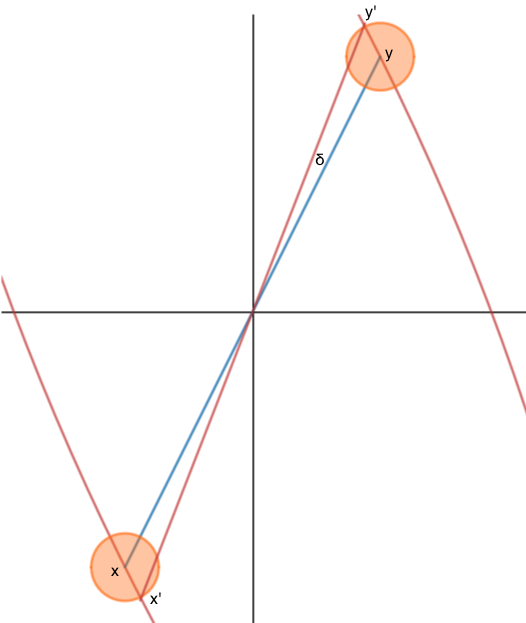
\includegraphics[scale=0.23]{convex-1.PNG}}
  \hfill
  \subfloat[Drawing for Lemma 3.2.1]{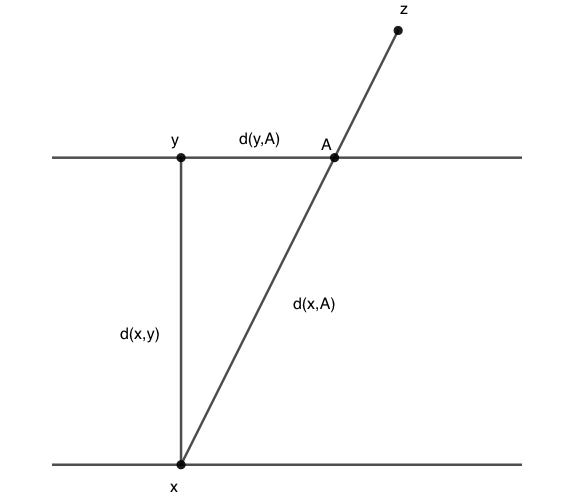
\includegraphics[scale=0.3]{line-1.PNG}}
\end{figure}

\begin{theorem}
If $K\subset \mathbb{R}^2$ is compact and convex, then $R_K(\theta)$ is continuous.
\end{theorem}
\begin{proof}
For let $K$ be compact and convex, and without loss of generality suppose it contained within the unit disc and contains the origin. Let $\theta\in (0,2\pi)$ be given and let $\ell_{\theta}$ be a line through the origin making an angle $\theta$ with the horizontal. Let $x=(x_1,x_2),y=(y_1,y_2)\in K$ be such that $W_{\ell_{\theta}}(K) = d(x,y)$. Such points exist as $K$ is compact. Let $\varepsilon>0$ be given. About $x$, consider $B_{\frac{\varepsilon}{2}}(x)$, and similarly $B_{\frac{\varepsilon}{2}}(y)$. Neither of these are empty, as $K$ is convex. Let $x',y'\in K\cap(B_{\frac{\varepsilon}{2}}(x)\cup B_{\frac{\varepsilon}{2}}(y))$ be such that $d(x',y')$ is maximized. As this set is compact, such points exist. Let $\delta = \min\{|\theta-\frac{x_2'}{\sqrt{x_1'^2+x_2'^2}}|,|\theta-\frac{y_2'}{\sqrt{y_1'^2+y_2'^2}}|\}$. Then for $|\theta-\theta_0|<\delta$, $d(x,y)-\varepsilon \leq W_{\ell_{\theta_0}}(K)\leq d(x,y)+\varepsilon$, and thus $|W_{\ell_\theta}(K)-W_{\ell_{\theta_0}}(K)| < \varepsilon$.
\end{proof}

\begin{lemma}
If $K$ is a compact subset of $\mathbb{R}^2$ and $x,y\in K$ such that $d(x,y)=D(K)$, then the lines perpendicular to $\overline{xy}$ at $x$ and $y$ contain all of $K$ in between.
\end{lemma}
\begin{proof}
Suppose not. Let $\overline{X}$ be the line perpendicular to $\overline{xy}$ containing point $x$, and similarly define $\overline{Y}$. Suppose there is a point $z\in K$ that falls on the exterior of the region $\mathcal{U} = \{(x,y)\in \mathbb{R}^2: (x,y)\ \textrm{Lies Between } \overline{X}\ \textrm{and } \overline{Y}\}$. Note that $d(x,z)\ne d(y,z)$, as then $z$ would line between these two lines. Suppose $d(y,z)<d(x,z)$. Where the line $\overline{xz}$ cuts $\overline{Y}$ denote as $A$. But then $d(x,z) > d(x,A) = \sqrt{d(y,A)^2+d(x,y)^2}\geq d(x,y)$. A contradiction as $d(x,y) = D(K)$. Thus $z\in \mathcal{U}$.
\end{proof}

\begin{theorem}
If $K\subset \mathbb{R}^2$ is compact and convex, then there are points $x,y\in K$ such that $\check{W}(K)=d(x,y)$.
\end{theorem}
\begin{proof}
As $f_K(\theta)$ is continuous for convex compact set, and as it is continuous on a compact set $[0,2\pi]$, it attains its maximum. Let $\theta$ be such a maximum. Let $\ell_{\theta}$ be the line through the origin which makes an angle $\theta$ with the horizontal axis and consider set $K_{\ell_{\theta}}$. As $K$ is compact and $\ell_{\theta}$ is closed, $K_{\ell_{\theta}}$ is compact. Then $W=\{d(x,y):x,y\in K_{\ell_{\theta}}\}$ is bounded, has a least upper bound, and therefore there are points $x,y \in K$ such that $\check{W}(K)=d(x,y)$.
\end{proof}

\begin{theorem}
If $K$ is a compact convex set of $\mathbb{R}^2$, then $D(K) = \check{W}(K)$.
\end{theorem}
\begin{proof}
As $K$ is compact, $D(K)$ and $\check{W}(K)$ exists and there are points $x,y$ such that $d(x,y) = D(K)$ and points $x',y'$ such that $d(x',y') = \check{W}(K)$. Suppose $d(x',y')> d(x,y)$. A contradiction, as $d(x,y)$ is the diameter of $K$. So $d(x,y) \geq d(x',y')$. Now suppose $d(x,y)>d(x',y')$. But as $d(x',y')= \check{W}(K)$, $d(x',y')$ is the greatest length of any line segment that terminates in $K$ and such that perpendiculars at these terminating points contain all of $K$. But as $d(x,y)=D(K)$, the lines perpendicular to $\overline{xy}$ at $x$ and $y$ contain all of $K$, a contradiction. Thus $d(x',y') \geq d(x,y)$. But it was just showed that $d(x,y)\geq d(x',y')$. Thus, $d(x,y) = d(x',y')$. $D(K) = \check{W}(K)$.
\end{proof}

\begin{definition}
If $Q$ is a convex polygon with interior (That is, positive area) in $\mathbb{R}^2$, then the perimeter of $Q$ is the sum of the lengths of its edges. 
\end{definition}

\begin{definition}
The perimeter of a line segment $e$ is $P(e) = 2|e|$.
\end{definition}

\begin{remark}
This is for the sake of continuity. If we take a rectangle of length $|e|$ and width $\frac{1}{n}$, then the perimeter is $2|e|+\frac{2}{n} \rightarrow 2|e|$ as $n\rightarrow \infty$. Thus, for the puprose of continuity we define the perimeter of line segments to be twice their length.
\end{remark}

\begin{theorem}[Cauchy's Perimeter Theorem]
If $K$ is a compact convex subset of the plane, then $P(K) = \pi W(K)$.
\end{theorem}
\begin{proof}
Suppose that $Q$ is a convex polygon with edges $e_1,\hdots, e_n$. At each $e_i$, let $\theta_i$ be the angle made with $e_i$ and the horizontal axis of $\mathbb{R}^2$. The mean width is $W(Q) = \frac{1}{2\pi}\int_{0}^{2\pi} W_{\ell_\theta}(Q)d\theta = \frac{1}{2\pi} \int_{0}^{2\pi} \frac{1}{2} \sum_{i=1}^{n} |e_i||\cos(\theta-\theta_i)|d\theta = \frac{1}{4\pi}\sum_{i=1}^{n} |e_i|\int_{0}^{2\pi} |\cos(\theta-\theta_i)|d\theta = \frac{1}{\pi} \sum_{i=1}^{n} |e_i| = \frac{1}{\pi} P(Q)$. Thus, $P(Q) = \pi W(Q)$. For any convex compact subset $K\subset \mathbb{R}^2$, we may find a polygon $Q$ that approximates the boundary with a perimeter $P(Q)$ that is as close to $P(K)$ and a width $W(Q)$ as close to $W(K)$ as desired. That is, for all $n\in \mathbb{N}$, we can obtain a polynomial $Q_n$ such that $\max\{|W(Q_n)-W(K)|,|P(K)-P(Q_n)|\}< \frac{1}{n}$. Then $|P(K)-\pi W(K)| = |P(K) - P(Q_n)+P(Q_n)-\pi W(Q_n)+\pi W(Q_n)-\pi W(K)| \leq |P(K)-P(Q_n)|+|P(Q_n)-\pi W(Q_n)|+\pi|W(Q_n)-W(K)| < \frac{1}{n} + 0 + \frac{\pi}{n} = \frac{1+\pi}{n} \rightarrow 0$. Thus, $P(K) = \pi W(K)$ for arbitrary convex compact subsets of the plane.
\end{proof}
 
\begin{theorem}
There exist compact path-connected sets $K\subset \mathbb{R}^2$ such that $P(K) \ne \pi W(K)$.
\end{theorem}
\begin{proof}
Consider the set $K = \{(x,y) \in \mathbb{R}^2: x^2+y^2=1, y\geq 0\}$. Then $P(K) = 2\pi$, but \\ $W(K) = \pi(\pi+2)$. To see this, consider the set $\mathcal{K} = \{(x,y)\in \mathbb{R}^2: x^2 + y^2 \leq 1, y\geq 0\}$. This is convex and has perimeter $\pi+2$ and therefore $W(\mathcal{K}) = \pi(\pi+2)$. But, as the image shows, $W(K) = W(\mathcal{K})$. That is, $W_{\ell_{\theta}}(K)$ is the length of the line segment $\overline{AB}$, as is $W_{\ell_{\theta}}(\mathcal{K})$. Therefore the averages $W(K)$ and $W(\mathcal{K})$ are the same. Thus, $P(K) \ne \pi W(K)$.
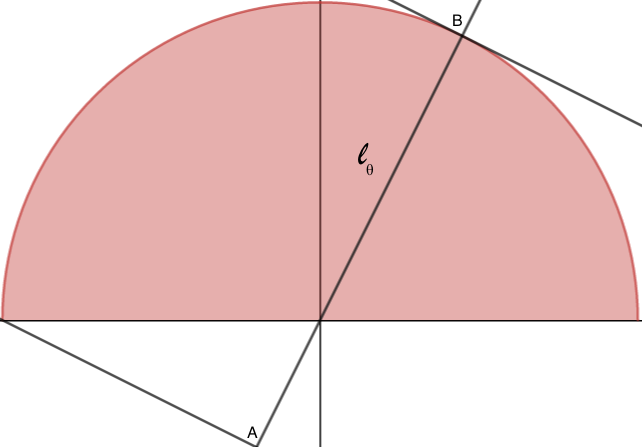
\includegraphics[scale=0.3]{semicircle-1.PNG}
\end{proof}

\begin{definition}
A functional $f$ with respect to subset inclusion is said to be monotonic on a family of sets $\mathscr{P}$ if and only if $f(K)\leq f(L)$ for all $K,L \in \mathscr{P}$ such that $K\subset L$.
\end{definition}

\begin{theorem}
If $K\subset L \in \mathscr{K}_2$, then $W_{\ell}(K) \leq W_{\ell}(L)$.
\end{theorem}
\begin{proof}
For let $\pi_{\ell}:\mathbb{R}^2 \rightarrow \ell$ be the orthogonal projection map of $\mathbb{R}^2$ to $\ell$. Then $\pi_{\ell}(K)\leq \pi_{\ell}(L)$ as $K\subset L$, and thus $W_{\ell}(K)\leq W_{\ell}(L)$.
\end{proof}

\begin{theorem}
If $K\subset L\in \mathscr{K}_2$, then $W(K)\leq W(L)$.
\end{theorem}
\begin{proof}
For $W_{\ell}(K)\leq W_{\ell}(L)$, and thus $W(K)=\frac{1}{2\pi}\int_{0}^{2\pi}W_{\ell_{\theta}}(K)d\theta \leq \frac{1}{2\pi}\int_{0}^{2\pi}W_{\ell_{\theta}}(L)d\theta=W(L)$.
\end{proof}

\begin{theorem}
If $K\subset L\in \mathscr{K}_2$, then $X_{\ell}(K)\leq X_{\ell}(L)$.
\end{theorem}
\begin{proof}
For if $x\in \ell\cap K$, then $x\in \ell\cap L$, and thus $X_{\ell}(K)=\mu(\ell\cap K) \leq \mu(\ell\cap L)=X_{\ell}(L)$.
\end{proof}

\begin{theorem}
If $K\subset L\subset \mathscr{K}_2$, then $D(K)\leq D(L)$.
\end{theorem}
\begin{proof}
For suppose not. Suppose $D(K)>D(L)$. Then, there are points $x,y\in K$ such that $d(x,y)> \sup\{d(x',y'):x',y'\in L\}$. But as $K\subset L$, $x,y\in L$ and thus $d(x,y) \not> \sup\{d(x',y'):x',y'\in L\}$. Thus, $D(K)\leq D(L)$.
\end{proof}

\begin{theorem}
If $K\subset L \subset \mathscr{K}_2$, then $R_K\leq R_L$.
\end{theorem}
\begin{proof}
For suppose not. Suppose $R_K>R_L$. But as $K\subset L$, either this circle contains all of $L$ as well or it doesn't. But then $R_L \not<R_K$. Thus, $R_L\geq R_K$.
\end{proof}

\begin{theorem}
If $K\subset L \in \mathscr{K}_2$, then $r_K \leq r_L$.
\end{theorem}
\begin{proof}
For suppose not. Suppose $r_K> r_L$. But as the inscribed circle of radius $r_K$ fits entirely in $K$, and $K\subset L$, then it fits inside of $L$. But then $r_K \not > r_L$. Thus, $r_L \geq r_K$.
\end{proof}

\begin{theorem}
If $K,L\in \mathscr{K}_2$ and $K\subset L$, then $P(K)\leq P(L)$.
\end{theorem}
\begin{proof}
As $K\subset L\in  \mathscr{K}_2$, $W(K)\leq W(L)$. As $K$ and $L$ are convex, $P(K)=\pi W(K)$ and $P(L)=\pi W(L)$. Thus, $P(K) \leq \pi W(L) = P(L)$. Therefore, $P(K)\leq P(L)$.
\end{proof}

\begin{theorem}
There exists sets $K,L\subset \mathbb{R}^2$ such that $L$ is convex, $K\subset L$, yet $P(K)>P(L)$.
\end{theorem}
\begin{proof}
For let $L = \{(x,y)\in \mathbb{R}^2: x^2 + y^2 \leq 1\}$. Then $P(L) = 2\pi$. Let $K = \{(x,y)\in \mathbb{R}^2: -\sqrt{2}x\leq y \leq \sqrt{2}x,\frac{-1}{\sqrt{3}} \leq x \leq \frac{1}{\sqrt{3}} \lor \sqrt{2}x\leq y \leq -\sqrt{2}x,\frac{-1}{\sqrt{3}} \leq x \leq \frac{1}{\sqrt{3}} \}$. $P(K) = 4(1+ \sqrt{\frac{2}{3}}) \approx 7.26>2\pi$.
\end{proof}

\begin{figure}[!h]
  \centering
  \subfloat[Drawing for Theorem 3.2.15]{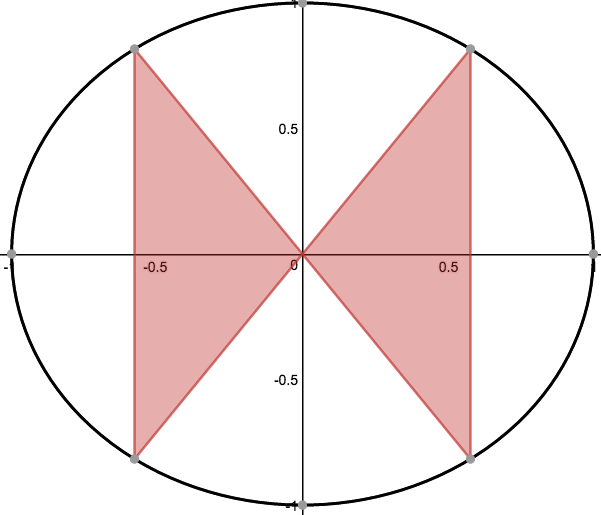
\includegraphics[scale=0.3]{Circles-3.PNG}}
  \hfill
  \subfloat[Drawing for Theorem 3.2.16]{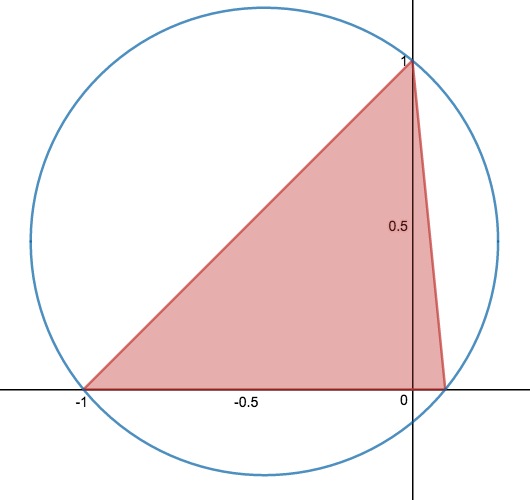
\includegraphics[scale=0.3]{Circle-4.PNG}}
\end{figure}

\begin{theorem}
There exist compact convex sets in $\mathbb{R}^2$ such that $D(K) < 2R_K$.
\end{theorem}
\begin{proof}
For consider the set $K=\{(x,y)\in \mathbb{R}^2: [0\leq y\leq x+1 \land x\geq 0]\lor [0\leq y\leq -10x+1\land x\geq 0]\}$. From Euclid, the smallest circle containing this triangle is the one defined by the three vertices (Three points define a triangle). This circle has the formula $(x+0.45)^2+(y-0.45)^2 = (0.45)^2 +(0.45+\frac{1}{10})^2$. Thus, $2R_K = \sqrt{0.45^2 +(0.45+\frac{1}{10})^2} > \sqrt{2} = D(K)$.
\end{proof}

\begin{theorem}
If $K$ is a compact convex set in $\mathbb{R}^2$, then $D(K) \leq 2R_K$.
\end{theorem}
\begin{proof}
For suppose not. Suppose $D(K) > 2R_K$. As $K$ is compact, there are points $x$ and $y$ in $K$ such that $d(x,y)=D(K)$. But then $d(x,y)>2R_K$, and thus at least one of $x$ or $y$ is not contained in the circle. A contradiction. Thus $D(K)\leq 2R_K$.
\end{proof}

\begin{theorem}
If $K$ is a compact convex set in $\mathbb{R}^2$, then $2\pi r_K \leq P(K)$.
\end{theorem}
\begin{proof}
From Calculus of Variations we know that the circle maximizes the area contained with a set of perimeter $p$. As the inscribed circle has perimeter $2\pi r_K$ and as the circle is a subset of $K$, it is true that $A(K)$ is greater than or equal the area of the circle. Thus, $P(K)\geq 2\pi r_K$.
\end{proof}

\begin{theorem}
For a compact convex set of $\mathbb{R}^2$, $P(K) \leq 2\pi R_K$.
\end{theorem}
\begin{proof}
As $K$ is convex, $P(K) = \pi W(K) \leq \pi \check{W}(K) = \pi D(K) \leq 2\pi R_K$.
\end{proof}

\begin{theorem}
If $K$ is a compact and convex subset of $\mathbb{R}^2$, then $2D(K)\leq P(K)$.
\end{theorem}
\begin{proof}
Suppose not. Suppose $2D(K) >P(K)$. As $K$ is compact and convex, there exist points $x,y\in K$ such that $d(x,y) = D(K)$. But as $K$ is convex, the line contained between $x,y$ in contained in $K$. Thus, $P(\overline{xy}) = 2D(K)$. But as $\overline{xy}\subset K$, $P(K)>P(\overline{xy})$, a contradiction. Thus, $2D(K) \leq P(K)$.
\end{proof}

\begin{theorem}
There exist compact convex subsets of $\mathbb{R}^2$ such that $2D(K) = P(K)$.
\end{theorem}
\begin{proof}
For take a straight line segment of length $\ell$. Then $D(K) = \ell$, $P(K) = 2\ell$, and thus $2D(K) = P(K)$.
\end{proof}

\begin{theorem}
If $K$ is a compact convex subset of $\mathbb{R}^2$, then $P(K) \leq \pi D(K)$.
\end{theorem}
\begin{proof}
From Cauchy's Perimeter theorem, $P(K) = \pi W(K) \leq \pi \check{W}(K) = \pi D(K)$.
\end{proof}

\begin{theorem}
For a compact convex subset $K$ of $\mathbb{R}^2$, $P(K) = \pi D(K)$ if and only if $W_{\ell}(K)$ is a constant.
\end{theorem}
\begin{proof}
For then $\frac{1}{2\pi} \int_{0}^{2\pi} W_{\ell_{\theta}}(K) d\theta = \check{W}(K)$. But as $W_{\ell_{\theta}}(K)$ is continuous for compact convex bodies, it must be true that $W_{\ell_{\theta}}(K) = \check{W}(K)$ for all $\ell_{\theta}$. Thus, $K$ is of constant width.
\end{proof}

\begin{remark}
There are many types of shapes that have constant width besides discs. The Reuleaux Triangle is such an example.
\end{remark}

Triangles are the simplest convex bodies in the plane other than points and lines. Any convex polygon can be written as the union of triangles with disjoint interiors. 

\begin{paracol}{2}
\begin{theorem}
If $\Delta_s$ is an equilateral triangle with edge length $s$, then $\Delta_s$ has the following properties:
\begin{enumerate}
\item $A(\Delta_s) = \frac{\sqrt{3}}{4}s^2$
\item $P(\Delta_s) = 3s$
\item $W(\Delta_s) = \frac{3s}{\pi}$
\item $R_{\Delta_s} = \frac{1}{\sqrt{3}}s $
\item $r_{\Delta_s} = \frac{1}{2\sqrt{3}}s $
\end{enumerate}
\end{theorem}
\switchcolumn
\begin{proof}
In order:
\begin{enumerate}
\item From Pythagoras, $A(\Delta_s) =2\times\big[\frac{1}{2}(\frac{1}{2}s)(\frac{\sqrt{3}}{2}s)\big] = \frac{\sqrt{3}}{4}s^2$
\item There are three edges, each of length $s$, and thus $P(\Delta_s) = 3s$.
\item $W(\Delta_s) = \frac{1}{\pi}P(\Delta_s) = \frac{3s}{\pi}$
\item The circumcircle gives the following equations:
\begin{enumerate}
\item $R_{\Delta_s}^2=\frac{s^2}{4}+h^2$
\item $h+R_{\Delta_s} = \frac{\sqrt{3}}{2}s$
\end{enumerate}
This has solution $R_{\Delta_s}=\frac{1}{\sqrt{3}}s$
\item $r_{\Delta_s} = \frac{R_{\Delta_s}}{2}= \frac{1}{2\sqrt{3}}s$
\end{enumerate}
\end{proof}
\end{paracol}

\begin{theorem}
If $T$ is a triangle in the plane, then there is a linear transformation $\psi$ such that $\psi T$ is equilateral.
\end{theorem}
\begin{proof}
For let $T$ be a triangle with vertices $a=(x_1,y_1)$, $b=(x_2,y_2)$, $c=(x_3,y_3)$. Let $A = d(b,c)$, $B=d(a,c)$, and $C=d(a,b)$. Suppose If $A=B=C$, we are done. Thus, suppose $C\geq B >A$. At point $a$ and with radius $C$, construct the circle $b,c',d$, and point $b$ and with radius $C$, construct the circle $a,c',e$. If we can shift $c$ to $c'$ in a linear fashion, we are done. Let $\psi =$
\end{proof} 

\begin{theorem}
If $T$ is a triangle with edges $a,b,c$ and opposite angles $\alpha,\beta,\gamma$, respectively, then $A(T) = \frac{\sin(\alpha)}{2}bc = \frac{\sin(\beta)}{2}ac = \frac{\sin(\gamma)}{2}ab$
\end{theorem}
\begin{proof}
Suppose the triangle is acute. The proof is symmetric for all sides, so we prove it for just $\alpha$. Note that the perpendicular $h$ dropped from the vertex of $a$ onto $b$ satisfies $h^2+\ell_1^2 = c^2$ and $h^2+\ell_2^2 = a^2$, where $\ell_1+\ell_2 = b$. Then $\sin(\alpha) = \frac{h}{c}$ and $A(T) = \frac{1}{2}h\ell_1 + \frac{h}{2}h\ell_2 = \frac{h}{2}(\ell_1+\ell_2)h = \frac{1}{2}bh = \frac{1}{2}bc\sin(\alpha)$. An identical argument works for obtuse triangles.
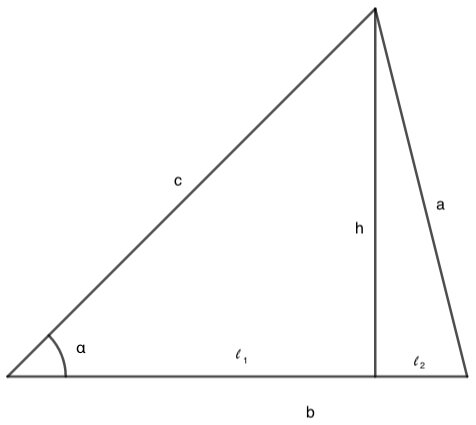
\includegraphics[scale=0.3]{triangle-1.PNG}
\end{proof}

\begin{corollary}[The Law of Sines]
For a triangle with edges $a,b,c$ and opposite angles $\alpha,\beta,\gamma$, $\frac{\sin(\alpha)}{a} = \frac{\sin(\beta)}{b} = \frac{\sin(\gamma)}{c}$
\end{corollary}
\begin{proof}
From the previous theorem, divide by $\frac{abc}{2}$ to obtain the result.
\end{proof}

\begin{theorem}[The Law of Cosines]
Given a triangle with lengths $a,b,c$ and opposite edges $\alpha,\beta,\gamma$, $c^2=a^2+b^2-2ab\cos(\gamma)$.
\end{theorem}
\begin{proof}
If $\gamma=\frac{\pi}{2}$, this is Pythagoras' Theorem. Thus, suppose $0<\gamma < \frac{\pi}{2}$. Where $c$ and $a$ meet, drop a perpendicular onto $c$ and call this $h$. $h$ satisfies $h^2+\ell_1^2 = c^2$ and $h^2+\ell_2^2=a^2$ from Pythagoras' Theorem, where $\ell_1+\ell_2 = b$. But $\ell_2 = a\cos(\gamma)$, so $\ell_1 = b-a\cos(\gamma)$. Thus $c^2 = h^2 + b^2 +a^2\cos^2(\gamma)-2ab\cos(\gamma)$. But $h = a\sin(\gamma)$. Thus, $c^2 = b^2 + a^2 \cos^2(\gamma)+\sin^2(\gamma)-2ab\cos(\gamma) = b^2 + a^2(\sin^2(\gamma)+\cos^2(\gamma))-2ab\cos(\gamma) = a^2 + b^2 -2ab\cos(\gamma)$. A similar construction is done if $\frac{\pi}{2}<\gamma < \pi$.
\end{proof}

\begin{theorem}
Given a triangle $\Delta$ with lengths $a\leq b\leq c$, $D(\Delta)=c$.
\end{theorem}
\begin{proof}
At the midpoint of $c$, and with radius $c$, construct a circle. This circle contains the entirety of $\Delta$, and thus for all points $x,y\in \Delta$, $d(x,y)\leq c$. Thus, $c=D(\Delta)$.
\end{proof}

\begin{theorem}[Heron's Formula]
For a triangle with lengths $a,b,c>0$, $A(T)^2 = \frac{1}{16}(a+b+c)(-a+b+c)(a-b+c)(a+b-c)$.
\end{theorem}
\begin{proof}
For $A(T) = \frac{1}{2}ab \sin(\gamma) = \frac{1}{2}ab\sqrt{1-\cos^2(\gamma)} = \frac{1}{4}\sqrt{4a^2 b^2 - (a+b-c)^2}=\\ \frac{1}{4}\sqrt{(2ab-(a^2+b^2-c^2))(2ab+(a^2+b^2+c^2))} = \frac{1}{4}\sqrt{(c^2-(a-b)^2)((a+b)^2-c^2)} = \\ \frac{1}{4}\sqrt{(a+b+c)(-a+b+c)(a-b+c)(a+b-c)}$. Squaring this gives the result.
\end{proof}

\begin{theorem}
For any triangle $\Delta$, $r_{\Delta}P(\Delta) = 2A(\Delta)$.
\end{theorem}
\begin{proof}
For let $\Delta$ has sides $a,b,c$, with opposite angles $\alpha, \beta, \gamma$, respectively. Then $A(\Delta) = \frac{ab}{2}\sin(\gamma)$ and $P(\Delta)=a+b+c$. Thus, $\frac{2A(\Delta)}{P(\Delta)} = \frac{ab\sin(\gamma)}{a+b+c}$. But this is the radius of the incircle of $\Delta$. Therefore, etc.
\end{proof}

\begin{theorem}[Viviani's Theorem: Page 17]
\end{theorem}

\begin{theorem}
There exist convex polygon's such that the inradius is not unique.
\end{theorem}
\begin{proof}
For consider the rectangle $[0,2]\times [0,1]$. The diameter of any circle that sits inside this body must be at most $1$, and thus the radius is at most $\frac{1}{2}$. However, there are multiple circles that achieve this. For example $(x-\frac{1}{2})^2+(y-\frac{1}{2})^2=\frac{1}{2}$ and $(x-\frac{3}{2})^2+(y-\frac{3}{2})^2=\frac{1}{2}$.
\end{proof}

\begin{theorem}
For an acute triangle, $\frac{2(A)}{abc} = \frac{1}{R_T}$.
\end{theorem}

\begin{theorem}
If $\Delta$ is a triangle with vertices $A,B,C$ and sides $a,b,c$, then given a circle that contains $A,B,C$, the radius of this circle $R$ satisfies $\frac{1}{R} =\frac{2A(\Delta)}{abc}$
\end{theorem}

\begin{definition}
If $K\in \mathscr{K}_2$, then $-K = \{-x:x\in K\}$.
\end{definition}

\begin{theorem}
If $K\in \mathscr{K}_2$, then $W_{\ell}(K) = W_{\ell}(-K)$.
\end{theorem}
\begin{proof}
For let $x,y\in K$ be such that $d(x,y) = W_{\ell}(K)$. Then $d(-x,-y) = W_{\ell}(-K) = d(x,y)$. Therefore, etc.
\end{proof}

\begin{theorem}
There exist sets $K$ and $L$ such that $W_{\ell}(K)<W_{\ell}(L)$ for all $\ell$ yet $K\not\subset L$ for any translation or rotation of $K$.
\end{theorem}

\begin{definition}
For $K\in \mathscr{K}$ and unit vector $u$, $\bar{X}_{u}(K)$ is the mean value of $X_{\ell}(K)$ over all lines $\ell$ parallel to $u$ such that $X_{\ell}(K)>0$.
\end{definition}

\begin{theorem}
For $K\in \mathscr{K}_2$, $\bar{X}_{u}(K) = W_{\ell}(K)=A(K)$.
\end{theorem}


\chapter{Some More Stuff}

\section{On the Quotients of Primes}
\begin{theorem}
The set of rational numbers $\frac{p}{q}$ where $p$ and $q$ are prime is dense in $\mathbb{R}^{+}$.
\end{theorem}
\begin{proof}
If $x=0$, from Euclid we have $\frac{1}{p_n}\rightarrow 0$, where $p_n$ is the $n^{th}$ prime. Let $x\in\mathbb{R}^{+}$ be given. From the Prime Number Theorem, $\frac{p_n}{n\ln(n)}\rightarrow 1$. Let $p_{\ceil{nx}}$ be the $\ceil{nx}^{th}$ prime. Then $\frac{p_{\ceil{nx}}}{p_n}\frac{n\ln(n)}{nx\ln(nx)}\rightarrow 1$. But $\frac{n\ln(x)}{nx\ln(nx)}\rightarrow \frac{1}{x}$. Therefore $\frac{p_{\ceil{nx}}}{p_n}\rightarrow x$.
\end{proof}

\section{On Uniform Convergence}

\begin{definition}
A sequence of functions $f_n$ is said to converge point-wise on a set $A$ to a function $f$, if $\forall\varepsilon>0$ and $\forall x\in A$, there is an $N\in\mathbb{N}$ such that $n>N \Rightarrow |f(x)-f_n(x)|<\varepsilon$.
\end{definition}

\begin{definition}
A sequence of functions $f_n$ converge uniformly on a set $A$ to $f$ if and only if $\forall \varepsilon>0$ $\exists N\in\mathbb{N}$ such that $\forall x \in A$ and $n>N$, $|f(x) -f_n(x)|<\varepsilon$.
\end{definition}

\begin{definition}
A sequence of functions $f_n$ are point-wise equicontinuous on a set $A$ if and only if $\forall \varepsilon>0, \forall x \in A,\ \exists \delta>0\ \forall n\in\mathbb{N}|\ |x-x_0|<\delta \Rightarrow |f_n(x) - f_n(x_0)|<\varepsilon$.
\end{definition}

\begin{definition} A sequence of functions $f_n$ are uniformly equicontinuous on a set A if and only if $\forall\varepsilon>0,\ \exists \delta>0\ \forall x\in A\ \forall n\in\mathbb{N}|\ |x-x_0|<\delta \Rightarrow |f_n(x) - f_n(x_0)|<\varepsilon$.
\end{definition}

\begin{definition} A subset $A$ of the real line is open if $\forall x\in A,\ \exists r>0|\ \forall y \in (x-r,x+r),\ y\in A$.
\end{definition}

\begin{definition}
An open cover $\Delta$ of a set $A\subset S$ is a set of open subsets $A_k\subset S$, such that $A \subset \cup_{k\in I} A_k$, where $I$ is some index, countable or uncountable.
\end{definition}

\begin{definition}
A set $A$ is said to be compact if and only if for all open coverings $\Delta$ there is a finite sub-cover $\Delta_0\subset \Delta$, such that $A\subset \cup_{A_k \in \Delta_0} A_k$.
\end{definition}

\begin{theorem}[Heine-Borel Theorem]
Any closed-bounded subset of the real line is compact. 
\end{theorem}
\begin{proof}
For let $A$ be a closed and bounded subset of $\mathbb{R}$ with least upper bound $b$ and greatest lower bound $a$. Let $\Delta$ be an open covering, and let $X$ be the set of points $y\in A$ such that for all $s<y$ such that $s\in A$, there is a finite refinement of $\Delta$ which covers these points. $X$ is non-empty, as $a\in X$. The set $X$ is bounded, as for all points $y\in X$ we have that $a\leq y \leq b$. As bounded sets have a least upper bound, let $x$ be the least upper bound. Suppose $x<b$. As $x\in [a,b]$, there exists an element $A_k$ of $\Delta$ such that $x \in A_k$. But as $A_k$ is open and therefore there is an $r>0$ such that $y\in (x-r,x+r)\Rightarrow y \in A_k$. But then $y=x + \frac{r}{2} > x$ and $y\in A_k$. Therefore x is not the least upper bound as we have found an element in $X$ greater than $x$. Therefore $x\not<b$. And thus $x=b$.
\end{proof}

\begin{theorem}
If a sequence of functions are point-wise equicontinuous on a closed and bounded set, then they are uniformly equicontinuous.
\end{theorem}
\begin{proof}
For let $A$ be a closed bounded subset of $\mathbb{R}$, and let $f_n(x)$ be a sequence of point-wise equicontinuous functions on $A$. As the set is closed and bounded, it is compact by the Heine-Borel theorem. Let $\varepsilon>0$ be given. For $x\in A$, define the function $\delta(x) = \min\{\sup\{\delta>0:\ |x-x_0|<\delta,\ x_0\in A \Rightarrow |f_n(x)-f_n(x_0)|<\frac{\varepsilon}{2}, \forall n\in\mathbb{N}\},b-a\}$. Construct the open covering $\mathcal{U}$ as follows: $\mathcal{U} = \{(x-\delta(x),x+\delta(x)):\ x\in A\}$. This is an open covering, as every set in $\mathcal{U}$ is open, and for all $x\in A$, $x\in(x-\delta(x),x+\delta(x))\in\mathcal{U}$. But as $A$ is compact, there is a finite sub-cover. Let $a=x_0<x_1<...<x_{n-1}<x_n=b$ be the centers of the remaining open sets in the sub-cover. Further refine this sub-covering as follows: If $(x_j-\delta(x_j),x_j+\delta(x_j))\subset (x_k-\delta(x_k),x_k+\delta(x_k))$ for $j\ne k$, then remove it from the sub-cover as it is superfluous. We now have a set of points $a=a_0<z_1<...<z_{N-1}<z_N=b$ such that $A \subset \cup_{i=0}^{N} (z_i-\delta(z_i),z_i+\delta(z_i))$. Let $\delta = \min\{\delta(z_0),...,\delta(z_N),\delta(b), \frac{(a+\delta(a)) - (z_1-\delta(z_1))}{2}, ..., \frac{(z_{N-1} + \delta(z_{N-1})) - (b-\delta(b))}{2}\}$. That is, $\delta$ is the smallest of the $\delta(z_i)$, or half of the smallest intersection of two consecutive intervals. Let $x\in A$ be arbitrary. If $(x-\delta,x+\delta)$ is contained entirely in one of the $(z_i-\delta(z_i),z_i+\delta(z_i))$ sets, then we have that $|x-x_0|<\delta \Rightarrow |x-x_0| <\delta(z_i) \Rightarrow |f_n(x)-f_n(x_0)|<\frac{\varepsilon}{2}$ for all $n\in\mathbb{N}$. Suppose that $(x-\delta,x+\delta)$ is contained in two of the $(x-\delta(z_i),x+\delta(z_i))$ sets. Note, it cannot be in three or more as we have refined the sub-cover in such a manner as to prevent this. Let $y$ be the center of the intersection of these two sets. Then we have that for $|x-x_0|<\delta$, then $|f_n(x)-f_n(x_0)| = |f_n(x) - f_n(y) + f_n(y) - f_n(x_0)| \leq |f_n(x) - f_n(y)| + |f_n(y) - f_n(x_0)|$. But $|x-y|$ and $|x_0-y|$ are less than $\frac{(z_i + \delta(z_i))-(z_{i+1}-\delta(z_{i+1}))}{2}$ apart, and therefore $|f_n(x) - f_n(y)|<\frac{\varepsilon}{2}$, and $|f_n(y) - f_n(x_0)| < \frac{\varepsilon}{2}$. Therefore, $|f_n(x) - f_n(x_0)|<\varepsilon$. And as $x$ is arbitrary, $f_n(x)$ is uniformly equicontinuous.
\end{proof}

\begin{theorem} If a sequence of point-wise equicontinuous functions converge, then the limit is point-wise continuous.
\end{theorem}
\begin{proof}
For let $f_n:A\rightarrow \mathbb{R}$ be equicontinuous, $\varepsilon>0$ and $x\in A$ be given. Choose $\delta>0$ to satisfy the criterion of equicontinuity at $x$. Let $x_0$ be an arbitrary point in $(x-\delta,x+\delta)\cap A$. It suffices to show that $|f(x) - f(x_0)|<\varepsilon$. As $f_n \rightarrow f$ we have that $\exists N_1 \in\mathbb{N}$ such that $n>N_1\Rightarrow |f(x) - f_n(x)|<\varepsilon$. We also have that $\exists N_2 \in \mathbb{N}$ such that $n>N_2 \Rightarrow |f(x_0)-f_n(x_0)|<\varepsilon$. Let $N=\max\{N_1,N_2\}+1$. But we have that $|f(x) - f(x_0)| = |f(x) - f_N(x) + f_N(x)-f_N(x_0) + f_N(x_0) - f(x_0)|\leq |f(x) - f_n(x)| + |f_n(x)-f_n(x_0)| + |f_n(x_0) - f(x_0)| < 3\varepsilon$. $f$ is continuous.
\end{proof}

\begin{theorem}
If $f_n \rightarrow f$ on a closed bounded subset of $\mathbb{R}$, and if $f_n$ is equicontinuous, then the convergence is uniform.
\end{theorem}
\begin{proof}
Let $A$ be a closed bounded subset of $\mathbb{R}$, $f_n(x)$ a sequence of equicontinuous functions, and let $\varepsilon>0$ be given. As $f_n(x)$ is equicontinuous on a closed bounded set, it is uniformly equicontinuous. But the limit of equicontinuous functions is continuous. Let $\delta>0$ be such that, $\forall x\in A$, $\forall n\in\mathbb{N}$, $|x-x_0|<\delta, x_0\in A \Rightarrow |f_n(x)-f_n(x_0)|<\frac{\varepsilon}{3}$ and $|x-x_0|<\delta \Rightarrow |f(x)-f(x_0)|<\frac{\varepsilon}{3}$. Let $\mathcal{U} = \{(x-\frac{\delta}{2},x+\frac{\delta}{2}): x\in A\}$. This is an open cover of $A$ and thus there is a finite subcover. Let $x_0<x_1<\hdots<x_n$ be the centers of the finitely many sets $(x_k-\frac{\delta}{2},x_k+\frac{\delta}{2})$ that cover $A$. There is thus another finite sequence of positive integers, $N_0, N_1,... N_n$, such that $n>N_k \Rightarrow |f(x_k)-f_n(x_k)|<\frac{\varepsilon}{3}$, for $k=0,1,2,...,n$. Let $N= \max\{N_0, N_1, ..., N_n\}$.It suffices to show that, for any point $x_0 \in A$, for all $n>N$, $|f(x_0)-f_n(x_0)|<\varepsilon$. Let $x_0$ be arbitrary and let $x_k$ be the nearest point to $x_0$ in the above sequence (If there are two nearest points, pick your favorite). Then we have that, for $n>N$, $|f(x_0) - f_n(x_0)| = |f(x_0)-f(x_k)+f(x_k)-f_n(x_k)+f_n(x_k)-f_n(x_0)|\leq |f(x_k)-f(x_0)|+|f(x_k)-f_n(x_k)|+|f_n(x_k)-f_n(x_0)|<\varepsilon$. The convergence is uniform.
\end{proof}


\begin{theorem}[Integration of a Uniformly Convergent Sequence of Functions] If $f_n\rightarrow f$ uniformly on a closed bounded set $A$ with $g.u.b(A)=a$, then $\int_{a}^{x} f_n \rightarrow \int_{a}^{x} f$ uniformly on $A$.
\end{theorem}
\begin{proof}
Let $\varepsilon >0$ be given, let $b=l.u.b.(A)$, and choose $N\in\mathbb{N}$ such that $n>N\Rightarrow |f(x)-f_n(x)|<\frac{\varepsilon}{b-a}$. Then we have $|\int_{a}^{x} f_n - \int_{a}^{x} f| = |\int_{a}^{x} (f_n-f)| \leq \int_{a}^{x} |f_n-f| < \int_{a}^{x} \frac{\varepsilon}{b-a}= \frac{\varepsilon}{b-a}(x-a) \leq \varepsilon$. 
\end{proof}

\begin{theorem}[Differentiation of a Uniformly Convergent Sequence of Functions]
If $f_n'\rightarrow g$ uniformly on a closed bounded set $A$, and if $f_n \rightarrow f$ on $A$, then $f' = g$.
\end{theorem}
\begin{proof} Let $a=g.u.b.(A)$ and $b=l.u.b.(A)$. We have that $f_n(x) - f_n(a) = \int_{a}^{x}f_n' \rightarrow \int_{a}^{x}g$ uniformly. But $f_n(x)-f_n(a) \rightarrow f(x) - f(a)$. Therefore $f'(x)=\frac{d}{dx}(f(x)-f(a)) = \frac{d}{dx}\int_{a}^{x} g = g(x)$. $f' = g$.
\end{proof}

\begin{theorem}[The Product of a Uniformly Convergence Sequence and a Bounded Function]  If $f_n \rightarrow f$ uniformly, and if $g$ is a bounded function, then $f_n g \rightarrow fg$ uniformly.
\end{theorem}
\begin{proof}
For let $\varepsilon>0$ and $x$ be given, and let $g$ be a bounded function with bound $M$, and choose $N\in\mathbb{N}$ such that $n>N \Rightarrow |f(x)-f_n(x)|<\frac{\varepsilon}{M}$. Then we have that $|f(x)g(x)-f_n(x)g(x)| = |g(x)||f(x)-f_n(x)| < M|f(x)-f_n(x)| <\varepsilon$.
\end{proof}

\begin{theorem}
If $f$ is continuous on a compact set $A$, then it is uniformly continuous.
\end{theorem}
\begin{proof}
For let $\varepsilon>0$ be given, let $a=g.u.b.(A)$, $b=l.u.b.(A)$, and for $x\in A$ define $\delta(x) = \min\{\sup\{\delta>0: |x-x_0|<\delta,x_0\in A\Rightarrow |f(x)-f(x_0)|<\frac{\varepsilon}{2}\},b-a\}$. Let $\Delta = \{(x-\delta(x),x+\delta(x)):x\in A\}$. Then $\Delta$ is an open cover of $A$ and therefore there is an open subscover. Let $x_k$ be the centers of the finitely many sets $(x_k-\delta(x_k),x+\delta(x_k))$ that cover $A$. Further refine this by removing overlaps. That is, if $(x_i-\delta(x_i),x_i+\delta(x_i))\subset (x_j-\delta(x_j),x_j+\delta(x_k))$ for $i\ne j$, then remove it for it is superfluous. We thus obtain a new sequence $z_1,\hdots, z_N$ such that the intervals $(z_k-\delta(z_k),z_k+\delta(z_k))$ cover $A$. Define $\delta = \min\{\delta(z_1),\hdots,\delta(z_N), \frac{(z_0+\delta(z_0))-(z_1-\delta(z_1))}{2},\hdots,(\frac{z_{N-1}+\delta(z_{N-1}))-(z_{N}-\delta(z_{N})}{2}\}$. Let $x,x_0\in A$ such that $|x-x_0|<\delta$. Let $x_k$ be the closest point in the sequence to $x$ (If there are two such points, pick your favorite). Then $|f(x)-f(x_0)|=|f(x)-f(x_k)+f(x_k)-f(x_0)|\leq |f(x)-f(x_k)|+|f(x_k)-f(x_0)|<\varepsilon$
\end{proof}

\begin{remark}
The proof of this is a mimicry of the proof that equicontinuity on a compact set implies uniform equicontinuity.
\end{remark}

\begin{definition}
A set $A$ is called sequentially compact if given a sequence $x_n\in A$, there is a convergent subsequence $x_{n_k}$.
\end{definition}

\begin{theorem}
Compact sets of $\mathbb{R}$ are sequentially compact.
\end{theorem}
\begin{proof}
Let $A$ be a compact set in $\mathbb{R}$, and let $x_n$ be a sequence in $A$. A point $x\in A$ is the limit of a subsequence of $x_n$ if for every $\varepsilon>0$ there are infinitely many of the $x_n$ such that $|x-x_n|<\varepsilon$. Suppose there is no such point. That is, for each $x\in A$ only finitely many of the $x_n$ lie within sufficiently small $\varepsilon-$neighborhoods. Let $\varepsilon(x) = \sup\{\varepsilon>0:\textrm{Only finitely many }x_n \textrm{ lie within } \varepsilon \textrm{ of } x\}$. Define $E=\{(x-\varepsilon(x)<x+\varepsilon(x)):x\in A\}$. This is an open cover of $A$, and therefore there is a finite subcover. Thus, at least one of the finitely many intervals $(x-\varepsilon(x),x+\varepsilon(x))$ must contain infinitely many of the $x_n$, a contradiction. Thus there is a convergent subsequence.
\end{proof}

\begin{theorem}
Continuous functions on compact sets are bounded.
\end{theorem}
\begin{proof}
For suppose not. Let $f:A\rightarrow \mathbb{R}$ be a continuous function on a compact set $A$, and let $x_n$ be a sequence of points in $A$ such that $f(x_n)>n$. Such a sequence must exist as $f$ is not bounded. As $A$ is compact, there must a point $x\in A$ such that some subsequence $x_{n_k}$ that converges to $x$. Let $\varepsilon >0$. Then, as $f$ is continuous, there is a $\delta>0$ such that $|x-x_0|<\delta,\ x_0\in A\Rightarrow |f(x)-f(x_0)|<\varepsilon$. But then for all points $x_{n_k}$ such that $|x-x_{n_k}|<\delta$, $-\varepsilon<f(x_{n_k})-f(x)<\varepsilon \Rightarrow f(x)-\varepsilon < f(x_{n_k})<f(x)+\varepsilon$. A contradiction as $f(x_{n_k})$ is unbounded. Thus, $f$ is bounded.
\end{proof}

\begin{corollary}
Continuous functions on compact sets attain their maximum and minimum.
\end{corollary}
\begin{proof}
For let $f:A\rightarrow \mathbb{R}$ be a continuous function on a compact set $A$. Let $f(A) = \{y\in \mathbb{R}:\exists x\in A|\ f(x)=y\}$. (This is called the image of $A$ under $f$). As $f$ is continuous, it is bounded, and thus the set $f(A)$ is bounded. But bounded sets have an l.u.b. and a g.u.b. Therefore, etc.
\end{proof}

\begin{lemma}[Uniform Limit Theorem]
If $f_n\rightarrow f$ uniformly, and if the $f_n$ are continuous, then $f$ is continuous.
\end{lemma}
\begin{proof}
For let $\varepsilon>0$ be given and let $x\in A$. Let $N\in \mathbb{N}$ such that $n>N$ implies $|f(\chi)-f_n(\chi)|<\frac{\varepsilon}{3}$ for all $\chi\in A$. Let $\delta>0$ be chosen such that $|x-x_0|<\delta, x_0\in A\Rightarrow |f_N(x)-f_N(x_0)|<\frac{\varepsilon}{3}$. Then  $|f(x)-f(x_0)|=|f(x)-f_N(x)+f_N(x)-f_N(x_0)+f_N(x_0)-f(x_0)|\leq |f(x)-f_N(x_0)|+|f_N(x)-f_N(x_0)|+|f(x_0)-f_N(x_0)|<\varepsilon$.
\end{proof}

\begin{theorem}
If $f_ng\rightarrow fg$ uniformly on a compact set $A$, and if $g$ is continuous and positive, then $f_n\rightarrow f$ uniformly.
\end{theorem}
\begin{proof}
As $g$ is positive on a compact set, its minimum is also positive and is attained on $A$. Let $x_{min}\in A$ be such a minimum of $g$. Let $\varepsilon>0$ be given and let $N\in \mathbb{N}$ be such that for $n>N$, $|f_ng-fg|<\varepsilon\cdot g(x_{min})$. Then, $|f_ng-fg|=|g||f_n-f|\leq |g(x_{min})||f_n-f|<\varepsilon \cdot g(x_{min})\Rightarrow |f_n-f|<\varepsilon$.
\end{proof}

\begin{lemma}
If $f_n'$ is uniformly bounded, then $f_n$ is equicontinuous.
\end{lemma}
\begin{proof}
For let $M$ be such a bound for $f_n'$ and let $\varepsilon>0$ be given. Choose $\delta = \frac{\varepsilon}{M}$. Then for $x,x_0\in A$ and $|x-x_0|<\delta$, $|\int_{x_0}^{x}f_n'| =|f_n(x)-f_n(x_0)| \leq \int_{x_0}^{x}|f_n'| \leq (x-x_0)M < \varepsilon$.
\end{proof}

\begin{theorem}
If $f_n'$ is uniformly bounded, and if $f_n \rightarrow f$ on a closed and bounded subset of $\mathbb{R}$, then the convergence is uniform.
\end{theorem}
\begin{proof}
From the previous lemma, $f_n$ is equicontinuous. But a sequence of equicontinuous functions on a compact set is uniformly equicontinuous. And a sequence of uniformly equicontinuous functions that converge does so uniformly. Therefore, etc.
\end{proof}

\begin{theorem}
If $f_n \rightarrow f$, $f_n'\rightarrow g$ and if $f_n''-f_n'$ is uniformly bounded on a closed bounded set, then the convergences are uniform and $f' = g$.
\end{theorem}
\begin{proof}
Let $A$ be the closed bounded set under consideration. First note that as $f''_n - f'_n$ is uniformly bounded, $f_n'-f_n$ is equicontinuous. But as $f_n'$ and $f_n$ converge to $g$ and $f$, respectively, then $f_n'-f_n$ converges to $g-f$ uniformly. Let $M$ be a bounded for $f_n''-f_n'$. Let $a$ be the greatest lower bound and $b$ be the least upper bound of $A$. We then have that $-Me^{-a}\leq e^{-x}[f_n''(x)-f_n'(x)]=\frac{d}{dx}[e^{-x}f_n'(x)] < Me^{-a}$. That is, $\frac{d}{dx}[e^{-x}f_n'(x)]$ is uniformly bounded, and therefore $e^{-x}f_n'(x)$ is equicontinuous. But equicontinuity on a compact set implies uniform equicontinuity. As $f_n'\rightarrow g$, and $e^{-x}$ is bounded on $A$, $e^{-x}f_n'\rightarrow e^{-x}g$. But a convergent uniformly equicontinuous sequence of functions converges uniformly. Thus, $e^{-x}f_n'(x) \rightarrow e^{-x}g(x)$ uniformly, and therefore, as $e^{-x}$ is continuous and positive on $A$, $f_n'(x)\rightarrow g(x)$ uniformly. But also $f_n'-f_n \rightarrow g-f$ uniformly, and therefore $f_n \rightarrow f$ uniformly. Thus, $f'=g$.
\end{proof}


\begin{corollary}
If $f_n' - f_n$ is uniformly bounded and if $f_n \rightarrow f$ on a closed and bounded set $A$, then the convergence is uniform.
\end{corollary}
\begin{proof}
Using the inequality from the previous theorem, let $M$ be a bound for $f_n'-f_n$ and let $a$ be the least upper bound of $A$. Then $-Me^{-a}\leq \frac{d}{dx}[e^{-x}f_n] \leq Me^{-a}$. Thus $e^{-x}f_n$ is uniformly equicontinuous and therefore $e^{-x}f_n\rightarrow e^{-x}f$ uniformly, and thus $f_n\rightarrow f$ uniformly.
\end{proof}

\begin{corollary}
If $f_n^{(N+1)}-f_n^{(N)}$ is bounded and a compact set, and if $f_n^{(k)}\rightarrow f_k$ for $k=0,1,\hdots, N$, then the convergence is uniform and $f_{k}' = f_{k+1}$ for $k=0,1,\hdots,N-1$.
\end{corollary}
\begin{proof}
A simple induction and application of the previous theorem proves this.
\end{proof}

\section{On Analyticity}

We deal with functions on intervals for simplicity.

\begin{definition}
A real-valued function $f$ is said to be smooth, denoted $f\in C^{\infty}$ if, for all $k$, $\frac{d^k}{dx^k}f(x) \equiv f^{(k)}(x)$ exists.
\end{definition}

\begin{theorem}[Taylor's Theorem]
If $f\in C^{\infty}$, on some interval $[a,b]$, and if $x_0\in (a,b)$, then $f(x) - \sum_{k=0}^{n} f^{(k)}(x_0)\frac{(x-x_0)^k}{k!} = \int_{x_0}^{x} f^{(n+1)}(t)\frac{(x-t)^n}{n!}dt$
\end{theorem}
\begin{proof}
We prove by induction. The base case says $f(x)-f(x_0) = \int_{x_0}^{x} f'(t)dt$, which is true. Suppose it holds for some $n\in \mathbb{N}$. Then $f(x)-\sum_{k=0}^{n+1} f^{(k)}(x_0)\frac{(x-x_0)^k}{k!} = f(x)-\sum_{k=0}^{n} f^{(k)}(x_0)\frac{(x-x_0)^k}{k!} - f^{(n+1)}(x)\frac{(x-x_0)^{n+1}}{(n+1)!} = \int_{x_0}^{x} f^{(n+1)}(t)\frac{(x-t)^n}{n!}dt - f^{(n+1)}(x)\frac{(x-x_0)^{n+1}}{(n+1)!}$. But $\int_{x_0}^{x} f^{(n+1)}(t)\frac{(x-t)^n}{n!}dt =  \int_{x_0}^{x} f^{(n+2)}(t) \frac{(x-t)^{n+1}}{(n+1)!} dt + f^{(n+1)}(x)\frac{(x-x_0)^{n+1}}{(n+1)!}$, from integration by parts. Thus, $f(x)-\sum_{k=0}^{n+1} f^{(k)}(x_0)\frac{(x-x_0)^k}{k!}= \int_{x_0}^{x} f^{(n+2)}(t) \frac{(x-t)^{n+1}}{(n+1)!} dt$
\end{proof}

\begin{lemma}
If $f\in C^{\infty}$ and $f^{(n)}(x)\rightarrow 0$ (Point-wise) on $[a,b]$, and if $F(x) \equiv f(x)-\sum_{k=0}^{\infty} f^{(k)}(x_0)\frac{(x-x_0)^{k}}{k!}$, where $x_0\in [a,b]$ is fixed, then $\int_{x_0}^{x} F^{(n+1)}(t)\frac{(x-t)^{n}}{n!}dt$ converges. 
\end{lemma}
\begin{proof}
For let $x,x_0\in [a,b]$ fixed. We will show that $\int_{x_0}^{x} F^{(n+1)}(t)\frac{(x-t)^{n}}{n!}dt$ is Cauchy. Let $\varepsilon>0$, $N_0 = 1$, and let $n>m>N_0$ be arbitrary. We have that $F(x) = \bigg(f(x)-\sum_{k=0}^{N} f^{(k)}(x_0)\frac{(x-x_0)^{k}}{k!}\bigg)-\bigg(g(x)-\sum_{k=0}^{N} f^{(k)}(x_0)\frac{(x-x_0)^{k}}{k!}\bigg)$, where $N\in \mathbb{N}$ is arbitrary. From Taylor's Theorem we thus have $F(x) = \int_{x_0}^{x}F^{N+1}(t)\frac{(x-t)^N}{N!}dt$. Then $|\int_{x_0}^{x}F^{n+1}(t)\frac{(x-t)^n}{n!}dt-\int_{x_0}^{x}F^{m+1}(t)\frac{(x-t)^m}{m!}dt| = |F(x)-F(x)|= 0 <\varepsilon$. 
\end{proof}

\begin{theorem}
If $f\in C^{\infty}$ and $f^{(n)}(x)\rightarrow 0$ (Point-wise) on some interval $[a,b]$, then $f^{(n)}(x)$ is uniformly bounded.
\end{theorem}
\begin{proof}
For let $x_0\in (a,b)$ be arbitrary. As $f^{(n)}(x_0)\rightarrow 0$, $\sum_{k=0}^{\infty} f^{(k)}(x_0)\frac{(x-x_0)^{k}}{k!}$ converges everywhere. Let $g(x)\equiv \sum_{k=0}^{\infty} f^{(k)}(x_0)\frac{(x-x_0)^{k}}{k!}$. Define $F(x) = f(x)-g(x)$. Then $F^{(n)}(x) = f^{(n)}(x)-g^{(n)}(x) = \bigg(f^{(n)}(x)-\sum_{k=n}^{N} f^{(k)}(x_0)\frac{(x-x_0)^{k}}{k!}\bigg)-\bigg(g^{(n)}(x)-\sum_{k=n}^{N} f^{(k)}(x_0)\frac{(x-x_0)^{k}}{k!}\bigg)$. From Taylor's theorem, this is equal to \\ $\int_{x_0}^{x} f^{(N+n+1)}(t)\frac{(x-t)^{N+n}}{(N+n)!}dt - \int_{x_0}^{x} g^{(N+n+1)}(t)\frac{(x-t)^{N+n}}{(N+n)!}dt = \int_{x_0}^{x} F^{(N+n+1)}(t)\frac{(x-t)^{N+n}}{(N+n)!}dt$. That is, for all $N>n$, $F^{(n)}(x) = \int_{x_0}^{x} F^{(N+n+1)}(t)\frac{(x-t)^{N+n}}{(N+n)!}dt$. But also $F^{(n)}(x)-\sum_{k=n}^{N} F^{(k)}(x_1)\frac{(x-x_1)^k}{k!} = \int_{x_1}^{x} F^{(N+n+1)}(t)\frac{(x-t)^{N+n}}{(N+n)!}dt$ for any point $x_1 \in (a,b)$. Now, suppose $f^{(n)}(x)$ is not uniformly bounded. $g^{(n)}(x)$ is uniformly bounded by its definition, and thus $F^{(n)}(x)$ is not uniformly bounded. Let ${k_n}$ be a subsequence of $n$ such that $F^{(k_n)}(x_{k_n})>n$. Such a sequence exists as $F^{(n)}(x)$ is not uniformly bounded. As $[a,b]$ is closed and bounded, it is compact. Thus $x_{k_n}$ has a convergent subsquence $\varphi(x_{k_n})$ (We use this notation so as to avoid writing $x_{k_{m_n}}$). Let $x_1$ be the limit of this subsequence. As $F^{(n)}(x_1)\rightarrow 0$, $\sum_{k=n}^{N} F^{(k)}(x_1)\frac{(x-x_1)^k}{k!}$ converges. Let $M$ be a bound for $F^{(k)}(x_1)$. (Such a bound exists as this sequence converges). We have that $F^{(n)}(x)-\sum_{k=n}^{N} F^{(k)}(x_1)\frac{(x-x_1)^k}{k!} = \int_{x_1}^{x} F^{(N+n+1)}(t)\frac{(x-t)^{N+n}}{(N+n)!}dt$. But $F^{(n)}(x) = \int_{x_0}^{x} F^{(N+n+1)}(t)\frac{(x-t)^{N+n}}{(N+n)!}dt$. Thus, $-\sum_{k=n}^{N} F^{(k)}(x_1)\frac{(x-x_1)^k}{k!} = \int_{x_0}^{x_1} F^{(N+n+1)}(t)\frac{(x-t)^{N+n}}{(N+n)!}dt$. Thus, $|\int_{x_0}^{x_1} F^{(N+n+1)}(t)\frac{(x-t)^{N+n}}{(N+n)!}dt|\leq Me^{b-a}$ for all $N$ and $n$. Thus $|F^{(n)}(x)| = |\int_{x_0}^{x} F^{(N+n+1)}(t)\frac{(x-t)^{N+n}}{(N+n)!}dt| = |\int_{x_0}^{x_1} F^{(N+n+1)}(t)\frac{(x-t)^{N+n}}{(N+n)!}dt+\int_{x_1}^{x} F^{(N+n+1)}(t)\frac{(x-t)^{N+n}}{(N+n)!}dt| \leq Me^{b-a}+|\int_{x_1}^{x} F^{(N+n+1)}(t)\frac{(x-t)^{N+n}}{(N+n)!}dt|$. But as $N$ is arbitrary, we may take it to be large enough to make the latter term close to a fixed finite value for each point. Thus $F^{(n)}(\varphi(x_{k_n}))\not\rightarrow \infty$ and therefore $F^{(n)}(x)$ is not unbounded, and is therefore uniformly bounded. Thus $f^{(n)}(x)$ is uniformly bounded.
\end{proof}

\begin{definition}
A function is said to be analytic at a point $x_0$ if $f(x) = \sum_{n=0}^{\infty} f^{n}(x_0) \frac{(x-x_0)^{n}}{n!}$. For all $x$ in the domain of $f$.
\end{definition}

\begin{theorem}[Lagrange's Remainder Theorem]
A function $f(x)$ is analytic if and only if $\int_{x_0}^{x}f^{n+1}(t)\frac{(x-t)^n}{n!}dt\rightarrow 0$.
\end{theorem}
\begin{proof}
For if $f(x)$ is analytic, then $f(x)-\sum_{k=0}^{n} f^{(k)}(x_0)\frac{(x-x_0)^n}{n!} = \int_{x_0}^{x}f^{n+1}(t)\frac{(x-t)^n}{n!}dt \rightarrow 0$. If $\int_{x_0}^{x}f^{n+1}(t)\frac{(x-t)^n}{n!}dt\rightarrow 0$, then $f(x)-\sum_{k=0}^{n}f^{(k)}\frac{(x-x_0)^{k}}{k!}\rightarrow 0$, and thus $f(x)$ is analytic.
\end{proof}

\begin{lemma}
If $f\in C^{\infty}$ and $f^{(n)}$ is uniformly bounded, then it is analytic.
\end{lemma}
\begin{proof}
For $|\int_{x_0}^{x}f^{n+1}(t)\frac{(x-t)^n}{n!}dt|\leq \int_{x_0}^{x}|f^{n+1}(t)||\frac{(x-t)^n}{n!}|dt$. As $f^{(n)}(x)$ is uniformly bounded, and for all $x$ $\frac{(x-x_0)^n}{n!} \rightarrow 0$, we have that $\int_{x_0}^{x}f^{n+1}(t)\frac{(x-t)^n}{n!}dt\rightarrow 0$.
\end{proof}

\begin{corollary}
If $f^{(n)}(x)\rightarrow 0$, then $f$ is analytic.
\end{corollary}
\begin{proof}
For $f^{(n)}(x)$ is thus uniformly bounded, and therefore analytic.
\end{proof}

\section{On Infinite Order O.D.E.'s}

\begin{definition}
An infinite order O.D.E. is a differential equation with no largest order of derivative.
\end{definition}

\begin{remark}
An infinite order O.D.E. then necessarily has an infinite number of terms.
\end{remark}

\begin{definition}
A linear infinite order O.D.E. is a differential equation of the form $\sum_{n=0}^{\infty} a_n(x) \frac{d^n f}{dx^n} = F(x)$.
\end{definition}

\begin{remark}
Unlike normal differential equation of order $n\in \mathbb{N}$, infinite order differential equations have the problem of convergence. That is, $\sum_{n=0}^{\infty} a_n(x) \frac{d^n f}{dx^n} = F(x)$ may have a different solution set if point-wise convergence is considered rather than uniform.
\end{remark}

We now consider the main topic of the paper.

\begin{proposition}
Consider the following differential equation on some interval $(a,b)$:
\begin{equation}
\nonumber \sum_{n=0}^{\infty} \frac{d^n f}{dx^n} = 0
\end{equation}
Be the convergence uniform or point-wise, the only solution is $f(x)=0$
\end{proposition}

We will prove this via the tools we have developed in the previous sections. First, some preliminary results.

\begin{theorem}
If, for some open set $A$, $f:A\rightarrow \mathbb{R}$ is continuous and positive at some point $x_0$, then there exists and open interval $(a,b)$ that contains $x_0$ such that $f(x)>0$ on this interval.
\end{theorem}
\begin{proof}
For let $A$ be open, let $f:A\rightarrow \mathbb{R}$ be continuous, and let $x_0\in A$ be such that $f(x_0)>0$. Let $\varepsilon = f(x_0)>0$. As $f$ is continuous, there is a $\delta>0$ such that $|x-x_0|<\delta$ and $x\in A$ implies $|f(x_0)-f(x)|<\varepsilon = f(x_0)$. As $A$ is open and $x_0\in A$ there is an $r>0$ such that $(x_0-r,x_0+r)\in A$. Then $(x_0-r,x_0+r)\cap (x_0-\delta,x_0+\delta)$ is an open interval in $A$ such that $0<f(x)<2f(x_0)$.
\end{proof}

\begin{theorem}[The Fundamental Theorem of the Calculus of Variations]
If $f$ is a continuous function on $(a,b)$, and if for all $\alpha,\beta\in (a,b)$ $\int_{\alpha}^{\beta}f = 0$, then $f=0$.
\end{theorem}
\begin{proof}
For suppose not. Let $f$ be positive at some point $x$. Then, as $f$ is continuous, there is a $\delta>0$ such that for all $x_0\in (x-\delta,x+\delta)\cap(a,b)$, $f(x_0)>0$. But then the integral on this subinterval is positive, a contradiction. Thus $f=0$.
\end{proof}

\begin{theorem}[Cauchy Criterion]
If $\sum a_n$ converges, then $a_n \rightarrow 0$.
\end{theorem}
\begin{proof}
For let $s_n$ be the $n^{th}$ partial sum. As convergent sequence are Cauchy sequences, $s_{n+1}-s_n \rightarrow 0\Rightarrow a_{n+1}\rightarrow 0$.
\end{proof}

\begin{theorem}
If $\sum_{n=0}^{N} \frac{d^{n}f}{dx^n} \rightarrow 0$ uniformly on some interval $(a,b)$, then $f=0$.
\end{theorem}
\begin{proof}
For any $\alpha, \beta\in (a,b)$, $\int_{\alpha}^{\beta} \sum_{n=0}^{N} \frac{d^{n}f}{dx^n} \rightarrow \int_{\alpha}^{\beta} 0 = 0$. Thus, $\int_{\alpha}^{\beta} f + \sum_{n=0}^{N-1} \frac{d^n f}{dx^n}\bigg|_{\alpha}^{\beta} \rightarrow 0$. As the latter term tends to $0$, $\int_{\alpha}^{\beta} f = 0$. As $\alpha$ and $\beta$ are arbitrary, $f=0$.
\end{proof}

\begin{theorem}
If $\sum_{n=0}^{N} \frac{d^n f}{dx^n} \rightarrow 0$ point-wise on some interval $(a,b)$, then $f=0$.
\end{theorem}
\begin{proof}
Suppose not. Let $x\in (a,b)$ be such that $f(x)\ne 0$. Consider the interval $[\frac{a+x}{2},\frac{x+b}{2}]=[\alpha,\beta]$ and let $S_N =\sum_{n=0}^{N} \frac{d^n f}{dx^n}$. Note that $S_N' = S_{N+1}-f$. So $S_N' - S_N = f^{(n+1)}-f$, and thus $|S_N'-S_N| = |f^{(n+1)}-f|$. As $\sum_{n=0}^{N} \frac{d^n f}{dx^n}$ converges, $\frac{d^n f}{dx^n} \rightarrow 0$. But then $f^{(n)}(x)$ is uniformly bounded on $[\alpha,\beta]$. Let $M_1$ be such a bound. As $f$ is continuous on $[\alpha,\beta]$ it is bounded. Let $M_2$ be such a bound. Let $M=M_1+M_2$. Then $|S_N'-S_N| = |f-f^{(N+1)}|\leq M$. That is, $|S_N'-S_N|$ is uniformly bounded. Therefore $S_N$ converges uniformly to zero. But if the convergence is uniform, then $f=0$. A contradiction. Thus $f$ is not nonzero anywhere, and therefore $f=0$.
\end{proof}

\begin{remark}
$a$ and $b$ need not be finite. The theorem holds on all of $\mathbb{R}$. 
\end{remark}

\section{Other Results}

\begin{theorem}
A sum of $K$ continuous functions is continuous. 
\end{theorem}
\begin{proof}
For let $f_n$, $n=1,2,\hdots,K$ be continuous, let $x$ be a point in their domains, and let $\varepsilon>0$ be given. Then, there is a $\delta_n$ such that $|x-x_0|<\delta_n$, with $x_0$ also in the domain, implies $|f_n(x)-f_n(x_0)|<\frac{\varepsilon}{K}$. Let $\delta = \min\{\delta_1,\hdots,\delta_n\}$. Then $|\sum_{n=1}^{K}[f_n(x)-f_n(x_0)]| \leq \sum_{n=1}^{K}|f_n(x)-f_n(x_0)| < \sum_{n=1}^{K} \frac{\varepsilon}{K} = \varepsilon$.
\end{proof}

\section{An Interestingly Uninteresting Algebraic Structure}
\subsubsection{Properties}
\noindent We define a Pseudo-Field to be a set equipped with two operations $<S,\circ, *>$ satisfying the following axioms.
$\forall a,b,c \in S$
\begin{enumerate}
\item $a\circ b = b\circ a$ \hfill Commutativity of the First Operation
\item $a\circ (b\circ c)=(a \circ b)\circ c$ \hfill Associativity of the First Operation
\item $a*b = b*a$ \hfill Commutativity of the Second Operation
\item $a*(b*c) = (a*b)*c$ \hfill Associativity of the Second Operation
\item $a*(b\circ c)=(a\circ b)*(a\circ c)$ \hfill The Second Operation Distributes over the First Operation
\item $a\circ (b*c) = (a\circ b)*(a\circ c)$ \hfill The First Operation Distributes over the Second Operation
\item $\exists e_{\circ}\in S|\ e_{\circ}\circ a = a$ \hfill Identity of the First Operation
\item $\exists e_{*} \in S|\ e_{*}*a = a$ \hfill Identity of the Second Operation
\item For all $a\in S$ there is an $a^{-1}\in S$ called the Pseudo-Inverse such that:
\begin{enumerate}
\item $a*a^{-1} = e_{\circ}$
\item $a\circ a^{-1}=e_{*}$
\end{enumerate}
\end{enumerate}

\begin{theorem} The identities are unique
\end{theorem}
\begin{proof} For suppose not. Suppose $e_{\circ}$ and $e_{\circ}'$ are identities not equal to each other. But then $e_{\circ}=e_{\circ}\circ e_{\circ}'=e_{\circ}'$. So the two are not unequal, and thus the identity is unique. Similarly for $e_{*}$.
\end{proof}
\begin{theorem} $e_{\circ}$ and $e_{*}$ are pseudo-inverses of each other.
\end{theorem}
\begin{proof} From identity, $e_{\circ}\circ e_{*}=e_{*}$ and $e_{*}*e_{\circ}=e_{\circ}$
\end{proof}
\begin{theorem} For any $a\in S$, $a*e_{\circ}=e_{\circ}$ and $a\circ e_{*}=e_{*}$
\end{theorem}
\begin{proof} By the definition of pseudo-inverses, we have $a*e_{\circ}=a*(a^{-1}*a)$, and from associativity and commutativity $a*(a^{-1}*a)=(a*a)*a^{-1}$. But from identity, we have $(a*a)*a^{-1}=[(a*a)\circ e_{\circ}]*a^{-1}=[(a*a^{-1})\circ (a*a^{-1})]*a^{-1}$. From the distributive property, $[(a*a^{-1})\circ (a*a^{-1})]*a^{-1}=[a*(a\circ a^{-1})]*a^{-1}=(a*e_{*})*a^{-1}=a*a^{-1}=e_{\circ}$. Similarly for $a\circ e_{*}=e_{*}$
\end{proof}
\begin{theorem} For any $a\in S$, $a*a = a\circ a = a$.
\end{theorem}
\begin{proof} Let $a\in S$. Then $a=a*e_{*}=a*(a\circ a^{-1})=(a*a)\circ(a*a^{-1})=(a*a)\circ e_{\circ}=a*a$. Similarly, $a=a\circ a$.
\end{proof}
\begin{theorem} If $a\circ b = a*b = a$, then $b=a$. 
\end{theorem}
\begin{proof}
For $b = b*(a\circ a^{-1}) = (b*a)\circ(b* a^{-1})= a\circ (b* a^{-1}) = (a\circ b)*(a\circ a^{-1}) = a$.
\end{proof}
\begin{theorem} The pseudo-inverses are unique.
\end{theorem}
\begin{proof} For suppose not. Suppose $a^{-1}$ and $a'^{-1}$ are both pseudo-inverses for some $a\in S$ not equal to each other.  Then $a*a^{-1}=a* a'^{-1}=e_{\circ}$. And $a\circ a^{-1}=a\circ a'^{-1}=e_{*}$. So then $a^{-1}=a^{-1}*(a\circ a'^{-1})=(a^{-1}*a)\circ (a^{-1}*a'^{-1})$ from the distributive property. Thus, from the property of pseudo-inverses and identity $a^{-1}=e_{\circ}\circ (a^{-1}*a'^{-1})=a^{-1}*a'^{-1}$. Similarly, $a'^{-1}=a'^{-1}*(a\circ a^{-1})=(a'^{-1}*a)\circ (a'^{-1}*a^{-1})=a'^{-1}*a^{-1}$. But it was just proven that $a^{-1}=a'^{-1}*a^{-1}$. So $a^{-1}=a'^{-1}$. The pseudo-inverse is unique.
\end{proof}
\begin{theorem} If for some $a\in S$, if $a=a^{-1}$, then $a=e_{\circ}=e_{*}$
\end{theorem}
\begin{proof} For let $a\in S$ and let $a=a^{-1}$. Then $a=a*a=a*a^{-1}$ from theorem 1.4. So $a=a*a^{-1}=e_{\circ}$. Similarly, $a=a\circ a^{-1} = e_{*}$
\end{proof}
\begin{theorem} For $a\in S$, $(a^{-1})^{-1} =a$.
\end{theorem}
\begin{proof} For we have $a = a\circ (a^{-1}* (a^{-1})^{-1}) = (a\circ a^{-1})*(a\circ (a^{-1})^{-1}) =a \circ (a^{-1})^{-1}$. Similarly, $a = a* (a^{-1})^{-1}$. But if $a = a\circ (a^{-1})^{-1} = a*(a^{-1})^{-1}$, then $a = (a^{-1})^{-1}$.
\end{proof}
\begin{definition} For $a\in S$, an inverse, or normal inverse, of the First Operation is an element $b\in S$ such that $a\circ b=e_{\circ}$. An inverse of the Second Operation is similarly defined. The normal inverses are denoted $a^{*}$ and $a^{\circ}$.
\end{definition}
\begin{theorem} If $a\in S$ has a normal inverse for either operation, than it is unique.
\end{theorem}
\begin{proof} For suppose not. Let $a\in S$ have a normal inverse for the First Operation. That is, there is an $a^{\circ}\in S$ such that $a\circ a^{\circ}=e_{\circ}$ and let $a'^{\circ}$ be a second normal inverse not equal to the first. But then $a^{\circ}=a^{\circ}\circ e_{\circ}=a^{\circ}\circ (a\circ a'^{\circ})$ and from associativity we have $a^{\circ}=(a^{\circ}\circ a)\circ a'^{\circ}=a'^{\circ}$. Thus, the normal inverse is unique. Similarly if there is an inverse for the Second Operation
\end{proof}
\begin{theorem} If $a\in S$ has a normal inverse, say $a'$, for one operation, then $a^{-1}=a'^{-1}$.
\end{theorem}
\begin{proof} For let $a\in S$ have a normal inverse $a'$ for the First Operation. That is, $a\circ a' = e_{\circ}$. But $a' \circ a'^{-1}=e_{*}$, and from theorem 1.3 $a\circ e_{*}=e_{*}$. So $a\circ (a' \circ a'^{-1})=e_{*}$. And from theorem 1.4, $a\circ a=a$, so we have $(a\circ a)\circ (a'\circ a'^{-1}=a\circ (a\circ a')\circ a'^{-1}=a\circ a'^{-1}=e_{*}$. But $a\circ a^{-1}=e_{\circ}$. And pseudo-inverses are unique. Thus, $a^{-1}=a'^{-1}$. 
\end{proof}
\begin{theorem} The identities have normal inverses for their respective operations.
\end{theorem}
\begin{proof} As normal inverses are unique, it suffices to find inverses for both identities. But $e_{\circ}\circ e_{\circ}=e_{\circ}$, so $e_{\circ}$ is its own inverse for the First Operation. Similarly, $e_{*}*e_{*}=e_{*}$.
\end{proof}
\begin{theorem} \textbf{(The Not-A-Field Theorem)} Only the identities have normal inverses.
\end{theorem}
\begin{proof} For suppose not. Suppose $a\in S,\ a\ne e_{\circ},\ a\ne e_{*}$ and a has an inverse for the First Operation. That is $\exists a^{\circ}\in S|\ a\circ a^{\circ}=e_{\circ}$. But by theorem 1.4, $a\circ a^{\circ}=(a\circ a)\circ a^{\circ}$. By associativity, we have $e_{\circ}=a\circ a^{\circ} = a\circ (a\circ a^{\circ})=a\circ e_{\circ}=a$. Thus, $a=e_{\circ}$. But by hypothesis, $a\ne e_{\circ}$. Thus, there is no inverse for $a$. Similarly, a has no inverse for the Second Operation.
\end{proof}
\begin{theorem}
There exist pseudo-fields with only one element.
\end{theorem}
\begin{proof}
For let $e_{\circ} = e_{*}$, and let no other elements be in the set. 
\end{proof}
\begin{theorem}
A pseud-field has one element if and only if $e_{\circ} = e_{*}$.
\end{theorem}
\begin{proof}
For suppose there is another element $a \ne e_{\circ}$. But then $a \circ e_{\circ} = a$, but also $a \circ e_{\circ} = a \circ e_{*} = e_{*}$. So $a = e_{*}$. If there is only one element, then clearly $e_{\circ} = e_{*}$ as otherwise there would be two elements.
\end{proof}
\begin{definition} A generating set on a pseudo-field is a subset $g_S \subset S$ such that every element of $S$ can be written as a finite combination of elements in $g_S$ using $\circ$ or $*$.
\end{definition}
\begin{theorem}
The number of elements in a finite pseudo-field is a power of 2.
\end{theorem}
\begin{proof}
Consider the set of all generators $g_S$ on $S$. Clearly for all such generators, $1\leq |g_S|\leq |S|$. Let $G$ be the smallest generator, such that $|G| \leq |g_S|$ for any other given generator. 
\end{proof}

\section{An Almost Group}

\begin{definition}
A group is a set $G$ with an operation $*$ satisfying the following:
\begin{enumerate}
\item $a*(b*c) = (a*b)*c$ for all $a,b,c\in G$.
\item There is an $e\in G$ such that $a*e=e*a = a$ for all $a\in G$.
\item For all $a\in G$ there is an $a^{-1}\in G$ such that $a*a^{-1}=a^{-1}*a = e$.
\end{enumerate}
\end{definition}

\begin{theorem}
The identity of a group is unique.
\end{theorem}
\begin{proof}
Suppose not, and let $e'$ be a different identity. But $e' = e'*e = e$. Thus $e$ is unique.
\end{proof}

\begin{definition}
A quasigroup is a group but the operation need not be associative.
\end{definition}

\begin{definition}
An Abelian Quasigroup is a quasigroup with a commutative operation.
\end{definition}

An interesting thing to note is that $e$ is an identity for $all$ elements of $G$. There are, however, groups with elements $a,b$ such that $a*b = b*a = a$, and yet $b\ne e$. They key difference is that $a*b$ does not necessarily equal $a$ for $all$ $a\in G$. 

\begin{theorem}
There exist abelian quasigroups $\langle G,*\rangle$ with elements $a,b\in G$ such that $a*b = b*a = a$, yet $b\ne e$.
\end{theorem}
\begin{proof}
In a pathological construction, let $G=\mathbb{R}$. Consider the following operation:
$x* y = \begin{cases} (x+y)^2, & x,y\ne 0 \\ x, & y=0,x\ne 0 \\ y, & x=0,y\ne 0 \\ 0, & x,y=0 \end{cases}$.
The identity is zero. For $0*0 = 0$, and if $x\ne 0$, then $x*0 = 0*x = x$. The inverse is $-x$. For if $x\ne 0$, then $x*(-x) = (x-x)=0$. The operation is not associative, for $x*(y*z) = (x+(y+z)^2)^2 \ne ((x+y)^2+z)^2$, in general. For take $x=2$, $y=1$, and $z=1$. Then $x*(y*z) = 36$, but $(x*y)*z = 100$. It is, however, commutative. For if $x,y \ne 0$, then $x*y = (x+y)^2 = (y+x)^2 = y*x$. The case of either element being zero is identity, and thus commutative. Let $x=4$ and $y=-2$. Then $x*y = (4-2)^2 = 4=x$, $y*x = (-2+4)^2 = 4 = x$. Also, $4*(-6) = (-6)*4 = (4-2)^2 = (-2)^2 = 4$. Thus, $4$ has three "Identities," that is $0,-2,-6$. $4$ is the only element, for let $x \ne 0$. Then $y = x-\sqrt{x}$ and $y=-x-\sqrt{x}$ are also "Identities," for $x$. Thus, with the exception of $0$ and $1$, every positive element has three "Identites." Note that $-2$ is only an "Identity," for the elements $4$ and $1$. Thus, for any other elements $x*(-2) \ne -2$. Thus, $-2$ is not a true identity.
\end{proof}

\section{On Sequences}

\subsubsection{Some Fun Stuff}

\begin{theorem}
Given an enumeration $\{x_n\}_{n=1}^{\infty}$ of the rationals $\mathbb{Q}\cap [0,1]$, for all $\varepsilon>0$ there is a $k\in \mathbb{N}$ such that $|x_{k+1}-x_k|<\varepsilon$.
\end{theorem}
\begin{proof}
For let $x_n$ be such an enumeration. Then, for all $n\in \mathbb{N}$, $0 \leq x_n \leq 1$.
\end{proof}

\begin{definition}
The Fibonacci Numbers are formed by the sequence $F_{n+2}=F_{n+1}+F_{n}$, with $F_0=F_1 = 1$.
\end{definition}

\begin{definition}
Two positive integers are said to be coprime if they share no common factors.
\end{definition}

\begin{theorem}
Any two consecutive Fibonacci numbers are coprime.
\end{theorem}
\begin{proof}
We have that $F_0=F_1 = 1$ and thus $F_2 = 2$, and also $F_3 = 3$. Suppose there is some integer $N\in \mathbb{N}$ such that $F_{N+2}$ and $F_{N+1}$ are not coprime. Then there is a least integer $n\in \mathbb{N}$ such that $F_{n+2}$ and $F_{n+1}$ are not corpime. That is, there are integers $a,b,c\in \mathbb{N}$ such that $F_{n+2} = ab$ and $F_{n+1} = ac$ where $b>c$. But then $F_{n} = F_{n+2} - F_{n+1} = a(b-c)$. Let $\alpha = b-c \in \mathbb{N}$. Then $F_n$ and $F_{n+1}$ are also not coprime. But this is impossible as $n$ is the least integer such that $F_{n+2}$ and $F_{n+1}$ are coprime, and $n-1<n$, a contradiction. Therefore there is no $N$ such that $F_{N+2}$ and $F_{n+1}$ are coprime. Consecutive Fibonacci numbers are coprime. 
\end{proof}

\begin{theorem}
For all $N\in \mathbb{N}$, $\sum_{n=1}^{N} n\cdot n! = (N+1)!-1$.
\end{theorem}
\begin{proof}
For $n\cdot n! = n\cdot n! + n! - n! = n!(n+1) - n!=(n+1)!-n!$. Thus, $\sum_{n=1}^{N} n\cdot n! = \sum_{n=1}^{N} (n+1)! -n! = (N+1)!-1$, as this is a telescoping series.
\end{proof}

\begin{theorem}
If $f(x)$ is an increasing function on $[1,N+1]$, then $\sum_{n=2}^{N+1} f(n) \leq \int_{1}^{N+1} f(x) \leq \sum_{n=1}^{N} f(n)$.
\end{theorem}
\begin{proof}
For $x\in [n,n+1]$, $f(n+1)\leq f(x)\leq f(n)$, as $f$ is decreasing. Thus $\int_{n}^{n+1} f(n+1)dx \leq \int_{n}^{n+1} f(x) dx \leq \int_{n}^{n+1} f(n)dx \Rightarrow f(n+1) \leq \int_{n}^{n+1}f(x)dx \leq f(n)$. Summing over this, we obtain $\sum_{n=1}^{N} f(n+1) \leq \int_{1}^{N+1} f(x) dx \leq \sum_{n=1}^{N} f(n)$. Finally, applying a shift of index to the leftmost term, $\sum_{n=2}^{N+1} \leq \int_{1}^{N+1}f(x)dx \leq \sum_{n=1}^{N} f(n)$. 
\end{proof}

\begin{corollary}
If $f$ is decreasing, then $\int_{1}^{n+1} f(x)dx \leq \sum_{k=1}^{n+1} f(k) \leq \int_{1}^{n+1} f(x)dx + f(1)$
\end{corollary}
\begin{proof}
From the previous theorem, $\int_{1}^{n+1}f(x) dx \leq \sum_{k=1}^{n}f(k)\leq \sum_{k=1}^{n+1}$. But also $\sum_{k=2}^{N+1} f(k) \leq \int_{1}^{n+1}f(x)dx$ so $\sum_{k=1}^{n+1}f(k) \leq \int_{1}^{n+1}f(x)dx +f(1)$. Combining these together gives the result.
\end{proof}

\begin{theorem}
$\underset{n\rightarrow \infty}\lim \sum_{k=1}^{n} \frac{1}{n+k} = \ln(2)$.
\end{theorem}
\begin{proof}
From the previous theorem, $\int_{1}^{n} \frac{1}{n+x} dx \leq \sum_{k=1}^{n} \frac{1}{n+k} \leq \frac{1}{n+1} + \int_{1}^{n} \frac{1}{n+x}dx$, and thus $\ln(n+x)\big|_{1}^{n+1} \leq \sum_{k=1}^{n} \frac{1}{n+k}\leq \frac{1}{n+1}+\ln(n+x)\big|_{1}^{n+1}\Rightarrow \ln(\frac{2n+1}{n+1})\leq \sum_{k=1}^{n} \frac{1}{n+k} \leq \ln(\frac{2n+1}{n+1})+\frac{1}{n+1}$. As $\frac{2n+1}{n+1}\rightarrow 2$ and as $\ln(x)$ is continuous, $\ln(\frac{2n+1}{n+1})\rightarrow \ln(2)$. But also $\frac{1}{n+1}\rightarrow 0$. Thus, by the squeeze theorem, $\sum_{k=1}^{n} \frac{1}{n+k} \rightarrow \ln(2)$.
\end{proof}

\begin{corollary}
$\sum_{k=1}^{n}\frac{1}{\sqrt{k}}< 2\sqrt{n}$.
\end{corollary}
\begin{proof}
From the theorem we have that $\sum_{k=1}^{n} \frac{1}{\sqrt{k}} \leq \int_{1}^{n}\frac{1}{\sqrt{x}}dx + 1 < \int_{1}^{n} \frac{1}{\sqrt{x}}dx +2 = 2\sqrt{n}-2+2 = 2\sqrt{n}$.
\end{proof}

\begin{lemma}
If $x\mod 1 < \frac{1}{2}$, then $2\floor{x} = \floor{2x}$.
\end{lemma}
\begin{proof}
Let $0\leq x \mod 1 \leq 0.5$. Then $0 \leq x-\floor{x}<0.5 \Rightarrow 2x-2\floor{x} <1$ and thus $2\floor{x} \leq \floor{2x} \leq 1+2\floor{x}$. But then we have that $0 \leq \floor{2x}-2\floor{x} <1$. But this is the difference of two integers, and is thus an integer. But there are no integers between $0$ and $1$, and therefore $\floor{2x}-2\floor{x} = 0$. Thus, $\floor{2x}=2\floor{x}$.
\end{proof}

\subsubsection{A Peculiar Family of Sequences and their Averages}

Consider the sequence $1,2,1,1,3,1,1,1,4,1,1,1,1,5,1,1,1,1,1,6,1,1,1,1,1,1,7,\hdots, n,\hdots (n\ 1's)\hdots, n+1,\hdots$, and also the generalization $1^k, 2^k,\hdots (2^k\ 1's)\hdots, 3^k, \hdots (3^k\ 1's)\hdots, 4^k, \hdots (4^k\ 1's)\hdots, 5^k,\hdots$\\

\begin{lemma}
If $a_n, b_n$ are sequences, $a_n\rightarrow A$ and $a_n-b_n\rightarrow 0$, then $b_n \rightarrow A$.
\end{lemma}
\begin{proof}
For $|A-b_n| \leq |A-a_n|+|a_n-b_n| \rightarrow 0$, thus $|A-b_n|\rightarrow 0$ and therefore $b_n \rightarrow A$.
\end{proof}

\begin{lemma}
Let $a_n$ be a sequence and $f,g$ be strictly increasing integer valued functions such that for all $m<f(n)$, $a_{f(n)}>a_m$ and for all $m>g(n)$, $a_{g(n)}<a_m$. If $a_{f(n)}\rightarrow A$ and $a_{f(n)}-a_{g(n)}\rightarrow 0$, then $a_n \rightarrow A$.
\end{lemma}
\begin{proof}
Let $\varepsilon>0$ be given. We have that $a_{g(n)}\rightarrow A$ as well from the previous lemma. Thus, there is an $N_1 \in \mathbb{N}$ such that for all $n>N_1$, $|A-a_{g(n)}|<\varepsilon$. Thus, for $n>N_1$, $A-\varepsilon < a_{g(n)}<A+\varepsilon$. But for all integers $n>g(N_1)$, $a_n >a_{g(N_1)}$, and thus $A-\varepsilon < a_n$ for all $n>g(N_1)$. As $a_{f(n)}\rightarrow A$, there is an $N_2$ such that for all $n>N_2$, $|A-a_{f(n)}|<\varepsilon$. Thus, for $n>N_2$, $A-\varepsilon < a_{f(n)}<A+\varepsilon$. As $f$ is a monotonically increasing function on the integers, $f(n)\geq n$. Thus, $a_{f(n)}>a_n$ for all $n$. But then for $n>\max\{g(N_1),N_2\}$, $A-\varepsilon < a_{g(n)} < a_n < a_{f(n)}<A-\varepsilon$. Thus, $a_n \rightarrow A$.
\end{proof}

\begin{lemma}
If $f$ and $g$ are continuous functions defined on $\mathbb{R}^+$, and if $\underset{x\rightarrow \infty}\lim f(x) = \underset{x\rightarrow \infty}\lim g(x)=A$, and if $S = \{(x,y):x\in \mathbb{R}^+,\min\{f(x),g(x)\}\leq y \leq \max\{f(x),g(x)\}\}$, and if $a_n$ is any sequence such that $(n,a_n)\in S$ for all $n\in \mathbb{N}$, then $a_n \rightarrow A$.
\end{lemma}
\begin{proof}
As $(n,a_n)\in S$, $\min\{f(n),g(n)\} \leq a_n \leq \max\{f(n),g(n)\} \Rightarrow 0 \leq a_n - \min\{f(n),g(n)\} \leq \max\{(f(n),g(n)\}-\min\{f(n),g(n)\}$. But $\max\{f(n),g(n)\}-\min\{f(n),g(n)\} \rightarrow 0$, and thus $a_n - \min\{f(n),g(n)\} \rightarrow 0$. From the lemma, $a_n \rightarrow A$.
\end{proof}

\begin{lemma}
If $P(x)$ and $Q(x)$ are polynomials of degree $n$, with leading coefficients $a_n$ and $b_n$, respectively, then $\underset{x\rightarrow \infty}\lim \frac{P(x)}{Q(x)} = \frac{a_n}{b_n}$.
\end{lemma}
\begin{proof}
From repeated application of L'H\^{o}pital's Rule, $\underset{x\rightarrow \infty}\lim \frac{P(x)}{Q(x)} = \underset{x\rightarrow \infty}\lim \frac{a_n x^n + \hdots + a_0}{b_n x^n + \hdots + b_0} = \underset{x\rightarrow \infty} \lim\frac{n! a_n}{n! b_n} = \frac{a_n}{b_n}$.
\end{proof}

\begin{theorem}
The average of the family of sequences we were considering is $2$. That is, let $a_n(k)$ be the $n^{th}$ term in the sequence $1^k, 2^k, \hdots (2^k\ 1's)\hdots,3^k,\hdots$, then the average $\frac{\sum_{n=1}^{N} a_n(k)}{N}$ converges to $2$ for all $k\geq 1$.
\end{theorem}

\section{A Class of Differentiability}

\begin{definition}
A function $f:(a,\infty)\rightarrow \mathbb{R}$, $a>0$, is said to be Kiwi Continuous if $f(x)-xf'(x)$ is bounded.
\end{definition}

\begin{remark}
A function is Kiwi Continuous if the set of $y-$intercepts of the tangent lines of $f(x)$ is bounded. 
\end{remark}

\begin{theorem}
If $f:[a,\infty)\rightarrow \mathbb{R}$ is Kiwi Continuous, then $f'$ is bounded.
\end{theorem}
\begin{proof}
By the definition, $-m \leq f(x)-xf'(x)\leq m$. Therefore $-\frac{m}{x^2} \leq \frac{f(x)}{x^2}- \frac{f'(x)}{x} \leq \frac{m}{x^2}$. But $\frac{f(x)}{x^2} - \frac{f'(x)}{x} = -\frac{d}{dx}\big(\frac{f(x)}{x}\big)$. So $-\frac{m}{x^2} \leq \frac{d}{dx}\big(\frac{f(x)}{x}\big) \leq \frac{m}{x^2}$. Let $x_0 \in (a,\infty)$. Then $-\int_{x_0}^x \frac{m}{\tau^2}d\tau = -\big[-\frac{m}{x}+ \frac{m}{x_0}\big] = \frac{m}{x}- \frac{m}{x_0} \leq \int_{x_0}^{x}\frac{d}{d\tau}\big(\frac{f(x)}{x}\big)d\tau = \frac{f(x)}{x} - \frac{f(x_0)}{x_0} \leq \int_{x_0}^{x} \frac{m}{\tau^2}d\tau = \frac{m}{x_0} - \frac{m}{x}$. So $\big|\frac{f(x)}{x}\big| \leq m|\frac{1}{x} - \frac{1}{x_0}| \leq m|\frac{2}{a}|$. Therefore $|f(x)| \leq 2\frac{m}{a}x$. But $|f(x) - xf'(x)| \leq m$. Thus $|f(x)-xf'(x)| \geq |f(x)| - x|f'(x)|$, and therefore $|f'(x)|  \leq \frac{m+|f(x)|}{x} \leq \frac{m+ \frac{2m}{a}x}{x} \leq \frac{m}{a} + \frac{2m}{a} = \frac{3m}{a}$. Therefore, $|f'(x)|$ is bounded.
\end{proof}

\part{Course Work: Physics}

\chapter{Electromagnetism I}

\section{Homeworks}

\subsection*{Homework I}

\subsubsection{Wangsness 1-2}

$\B{A} =  2\hat{x} - 3\hat{y} - 4\hat{z}$, $\B{B} = 6\hat{x} + 5\hat{y} + \hat{z}$, $\B{A+B} = 8\hat{x} + 2\hat{y} - 3\hat{z}$, $|\B{A+B}| = (8^2 + 2^2 + 3^3)^{1/2} = \sqrt{77}$ \\ $\B{A-B} = -4\hat{x} -8 \hat{y} - 5\hat{z},\ |\B{A-B}| = (4^2 + 8^2 + 5^2)^{1/2}=\sqrt{105}$ \\
$\B{a}\cdot \B{b} = |a||b|\cos(\theta) \Rightarrow \theta = \cos^{-1}\big(\frac{\B{a}\cdot \B{b}}{|a||b|}\big)$ The direction cosines of $\B{A+B}$ for $x,y,z$ are, respectively: \\
$\alpha = \cos^{-1}\big(\frac{(\B{A+B})\cdot \hat{x}}{|\B{A+B}|}\big)=24.3^{\circ},\ \beta = \cos^{-1}\big(\frac{(\B{A+B})\cdot \hat{y}}{|\B{A+B}|}\big)=76.8^{\circ},\ \gamma = \cos^{-1}\big(\frac{(\B{A+B})\cdot \hat{z}}{|\B{A+B}|}\big)=110^{\circ}$\\
For $\B{A-B}$:\\
$\alpha = \cos^{-1}\big(\frac{(\B{A-B})\cdot \hat{x}}{|\B{A-B}|}\big)=\frac{-4}{\sqrt{105}},\ \beta = \cos^{-1}\big(\frac{(\B{A-B})\cdot \hat{y}}{|\B{A-B}|}\big)=\frac{-8}{\sqrt{105}},\ \gamma = \cos^{-1}\big(\frac{(\B{A-B})\cdot \hat{z}}{|\B{A-B}|}\big)=\frac{-5}{\sqrt{105}}$ 

\subsubsection{Wangsness 1-3}

$\B{R} = \B{P}-\B{P'} = 5\hat{x} - 3\hat{y} - \hat{z}$. $|\B{R}| = (5^2+3^2+1^2)^{1/2} = \sqrt{35}$.\\
$\alpha = \cos^{-1}\big(\frac{5}{\sqrt{35}}\big) = 32.5^{\circ}$\\
$\beta = \cos^{-1}\big(\frac{-3}{\sqrt{35}}\big) = 120^{\circ}$\\
$\gamma = \cos^{-1}\big(\frac{-1}{\sqrt{35}}\big) = 99.7^{\circ}$

\subsubsection{Wangsness 1-4}

$\B{A} = \hat{x} + 2\hat{y} + 3\hat{y}$ $\ $  $\ $, $\ $  $\B{B} = 4\hat{x} - 5\hat{y} + 6\hat{z}$\ $\ $ \ ,$\ $ $\ $ $\theta = \cos^{-1}\big(\frac{\B{A}\cdot\B{B}}{|A||B|}\big) = \cos^{-1}\big(\frac{4-10+18}{\sqrt{14}\sqrt{77}}\big)=\cos^{-1}\big(\frac{12}{7\sqrt{22}}\big)=68.6^{\circ}$ \\
Components of $\B{A}$ in the direction of $\B{B}$:\\
$\B{A}\cdot \frac{\B{B}}{|B|} = |A|\cos(\theta) = \frac{12}{\sqrt{77}} \approx 1.37$

\subsubsection{Wangsness 1-5}

$\B{A} = 2\hat{x} + 3\hat{y} - 4\hat{z}$, $\ $ $\B{B} = -6\hat{x} - 4\hat{y} + \hat{z}$\\
$\B{A}\times \B{B} = \begin{vmatrix} \hat{x} & \hat{y} & \hat{z} \\ 2 & 3 & -4 \\ -6 & -4 & 1 \end{vmatrix} = (3-16)\hat{x} + (24-2)\hat{y} + (-8+18)\hat{z} = -13\hat{x} + 22\hat{y} + 10\hat{z}$ \\
Component along the direction of $\B{C} = \hat{x} - \hat{y} + \hat{z}$:\\
$(\B{A}\times \B{B})\cdot \frac{\B{C}}{|C|} = \frac{-13-22+10}{\sqrt{3}}=\frac{-25}{\sqrt{3}}$

\subsubsection{Wangsness 1-8}

$u = xy$, $\ $ $\nabla u = \hat{x}\frac{\partial u}{\partial x}= y\hat{x} + x\hat{y}$ \\
If $u = 3$ and $x=2$, then $y = \frac{3}{2}$\\
$\nabla u = \frac{3}{2}\hat{x} + 2\hat{y}$ \\
$\B{A} = 3\hat{x} + 2\hat{y} + 4\hat{z}$, $\ $ $\B{A}\cdot \frac{\nabla u}{|\nabla u|} = \frac{\frac{9}{2}+4}{\sqrt{(\frac{3}{2})^2 + 2^2}} = \frac{\frac{17}{2}}{\frac{5}{2}} = \frac{17}{2}\approx 3.4$


\subsubsection{Wangsness 1-9}

$u = \frac{x^2}{a^2} + \frac{y^2}{b^2} + \frac{z^2}{c^2}$ \\
$\nabla u = \frac{2x}{a^2}\hat{x} + \frac{2y}{b^2}\hat{y} + \frac{2z}{c^2}\hat{z}$\\
$\hat{n} = \frac{\nabla u}{|\nabla u|} = \frac{\frac{x}{a^2}\hat{x} + \frac{y}{b^2}\hat{y}+\frac{z}{c^2}\hat{z}}{\sqrt{\frac{x^2}{a^4}+\frac{y^2}{b^4}+\frac{z^2}{c^4}}}$


\subsection*{Homework II}

\subsubsection{Wangsness 1-11}

$\B{A} = x^2\hat{x}+y^2\hat{y}+z^2\hat{z}$. Along $z=0$, $\int_C \B{A}\cdot\B{dl} = \int_C(x^2 \hat{x}+y^2\hat{y})\cdot(dx\hat{x}+dy\hat{y}) = \int_C x^2 dx + \int_C y^2 dy$. The path $C$ says $y^2 = x,\ 2ydy = dx$. $\int_C \B{A}\cdot{dl} = \int_{0}^{\sqrt{2}}y^4(2ydy) +\int_{0}^{\sqrt{2}}y^2 dy =\int_{0}^{\sqrt{2}}y^2(2y^3+1)dy= \frac{2}{3}[4+\sqrt{2}]$. 

\begin{figure}[!h]
  \centering
  \subfloat[Path of Integration (Wangsness 1-11)]{\includegraphics[scale=0.4]{1-11.PNG}}
  \hfill
  \subfloat[The Geometry of the Problem (Wangsness 1-12)]{\includegraphics[scale=0.4]{1-12.PNG}}
\end{figure}

\subsubsection{Wangsness 1-12}

This is the hard way. For a very simple method, see below.
For a sphere of radius $a_0$, $x^2+y^2+z^2 = a_0^2$. $\B{r} = x\hat{i}+y\hat{j}+z\hat{k}$. Note: We are using $\hat{i},\hat{j},\hat{k}$ for $\hat{x},\hat{y},\hat{z}$, respectively. We have that $\underset{Sphere}\int \B{r}\cdot \B{da} = \underset{Sphere}\int\B{r}\cdot \hat{n}da$. Here it is in rectangular coordinates. It is much easier in spherical coordinates. The projection of $da$ on the $xy-plane$ is $da_z= \pm dxdy$. Throughout we have that $\hat{n} = \frac{x\hat{i}+y\hat{j}+z\hat{k}}{\sqrt{x^2+y^2+z^2}}$. In the upper hemisphere we have $da= \frac{dx dy}{\hat{n}\cdot \hat{k}}$, where $\hat{k}$ is the unit vector on the sphere normal to the $xy-plane$. That is, $\hat{k} = \frac{z}{\sqrt{x^2+y^2+z^2}}$. Thus we have $\underset{Upper Hemisphere}{\int \B{r}\cdot \hat{n} da} = \iint(x\hat{i}+y\hat{j}+z\hat{k})\cdot\big(\frac{x\hat{i}+y\hat{j}+z\hat{k}}{\sqrt{x^2+y^2+z^2}}\frac{dxdy}{\frac{z}{\sqrt{x^2+y^2+z^2}}}\big)=\iint (x\hat{i}+y\hat{j}+z\hat{k})\cdot (x\hat{i}+y\hat{j}+z\hat{k}\big)\frac{dxdy}{z}=\iint(x^2+y^2+z^2)\frac{dxdy}{z}$. But recall that $x^2+y^2+z^2=a_0^2$, and thus $z^2 = a_0^2 - x^2 - y^2$. So we have $\iint \frac{x^2+y^2+a_0^2-x^2-y^2}{\sqrt{a_0^2-x^2-y^2}}dxdy = \iint \frac{a_0^2}{\sqrt{a_0^2-x^2-y^2}}dxdy$. As $a_0^2$ is a constant, we may reduce this to $a_0^2\iint \frac{1}{\sqrt{a_0^2-x^2-y^2}}dxdy$. The region of integration is $-\sqrt{a_0^2-x^2}\leq y \leq \sqrt{a_0^2-x^2}$ and $-a_0\leq x \leq a_0$. So we obtain the definite integral $a_0^2 \int_{-a_0}^{a_0}\int_{-\sqrt{a_0^2-x^2}}^{\sqrt{a_0^2-x^2}} \frac{1}{\sqrt{a_0^2-x^2-y^2}}dxdy$. We solve this using trigonometric substitution to obtain $a_0^2 \sin^{-1}\big(\frac{y}{\sqrt{a_0^2-x^2}}\big)\bigg|_{-\sqrt{a_0^2-x^2}}^{\sqrt{a_0^2-x^2}} = \pi a_0^2$. Then $\int_{-a_0}^{a_0} \pi a_0^2 dx = 2\pi a_0^3$. This is the integral over the top half of the sphere. The lower half is the same integral but with different limits and a minus sign in $da$. The minus sign and the limits cancel and we get $\underset{Lower Hemisphere}{\int \B{r}\cdot \hat{n}da} = 2\pi a_0^3$. Thus, $\underset{Sphere}\int \B{r}\cdot \hat{n}da = 4\pi a_0^3$. \\ 
Using spherical coordinates is much easier. $\underset{Sphere}\int \B{r}\cdot \B{da} = \int_{0}^{2\pi}\int_{0}^{\pi} r\hat{r}\cdot \hat{r}(r^2 \sin(\theta) d\theta d\phi)$. On the sphere $r = a_0$, and thus we have $\int_{0}^{2\pi}\int_{0}^{\pi} a_0^3 \sin(\theta)d\theta d\phi = 4 \pi a_0^3$.\\
Using the divergence theorem is the simplest method.
$\nabla \cdot \B{r} = \frac{\partial x}{\partial x} + \frac{\partial y}{\partial y} + \frac{\partial z}{\partial z} = 1+1+1=3$. Thus $\iiint_V \nabla \cdot \B{r} d\tau = 3\iiint_V d\tau = 3\cdot(\textrm{Volume of a Sphere)} = 3 \frac{4}{3}\pi a_0^3=4\pi a_0^3$.\\
Remember that the divergence theorem says that for a closed surface $\partial V$ encompassing a volume $V$, $\oiint_{\partial V} \B{A}\cdot\B{da} = \iiint_{V} \nabla\cdot \B{A} d\tau$

\subsubsection{Wangsness 1-13}

\begin{figure}[htbp]
\begin{center}
\includegraphics[scale=0.3]{1-13.PNG}
\caption{Region of Integration}
\label{default}
\end{center}
\end{figure}

$\B{A}= xy\hat{i} + yz\hat{j} + xz\hat{j}$. $\nabla \cdot \B{A} = x+y+z$. Flux $= \Phi = \oiint \B{A}\cdot \B{da}$. There are six sides we must integrate over. Recall that in Cartesian coordinates, $\B{da} = \pm dydz \hat{i} \pm dxdz\hat{j} \pm dxdy\hat{k}$. Front face at $x=a$, $\iint(ay\hat{i}+yz\hat{j}+az\hat{k})\cdot \hat{i}dydz = \int_{0}^{c}\int_{0}^{b}aydydz = \frac{1}{2}ab^2c$. Backface at $x=0$, $\iint(0\hat{i}+yz\hat{j}+0\hat{k})\cdot (-\hat{i})dydz = 0$. Right face at $y=b$, $\iint(xb\hat{i}+bz\hat{j}+xz\hat{k})\cdot\hat{j}dxdz = \int_{0}^{c}\int_{0}^{a} bz dxdz = \frac{1}{2}ab c^2$. Along the left face $y=0$, $\iint(0\hat{i}+0\hat{j}+xz\hat{k})\cdot (-\hat{j})dxdz = 0$. Top face $z=c$, $\iint(xy\hat{i}+yc\hat{j}+xc \hat{k})\cdot \hat{k}dxdy = \int_{0}^{b}\int_{0}^{a} xcdxdy = \frac{1}{2}a^2bc$. Along the bottom face $z=0$, $\iint(xy\hat{i}+0\hat{j}+0\hat{k})\cdot (-\hat{k})dxdy = 0$. So, $\oiint \B{A}\cdot \B{da} = \frac{1}{2} a^2bc + \frac{1}{2}ab^2c + \frac{1}{2}abc^2 = \frac{abc}{2}(1+b+c)$. We now compute $\iiint_V \nabla \cdot \B{A} d\tau$. $\nabla \cdot \B{A} = x+y+z$. So $\iiint_V \nabla \cdot \B{A} d\tau = \iiint_V (x+y+z)d\tau = \int_{0}^{c}\int_{0}^{b}\int_{0}^{a}(x+y+z)dxdydz = \frac{abc}{2}(a+b+c) = \oiint \B{A}\cdot \B{da}$, in agreement with the divergence theorem.

\subsubsection{Wangsness 1-14}

$\B{A} = -y\hat{i}+x\hat{j}$. $\oint_C \B{A}\cdot \B{dl} = \oint_{C} (-y\hat{i}+x\hat{j})\cdot(\hat{i}dx+\hat{j}dy) = \oint_{c}(-ydx+xdy)$ Going along each path individually: \\
$\underbrace{\int_{0}^{3} (-ydx+xdy)}_\text{y=0,\ dy=0} = 0$, $\underbrace{\int_{0}^{4}(-ydx+xdy)}_\text{x=3,\ dx=0} = 12,\ \underbrace{\int_{3}^{0}(-ydx+xdy)}_\text{y = 4,\ dy=0}= 12,\ \underbrace{\int_{4}^{0}(-ydx+xdy)}_\text{x=0,\ dx=0} = 0$. Thus, $\oint_{C} \B{A}\cdot \B{dl} = 0+12+12+0 = 24$. We next compute $\iint (\nabla\times \B{A})\cdot \B{da}$\\ $\nabla \times \B{A} = \begin{vmatrix} \hat{i} & \hat{j} & \hat{k} \\ \frac{\partial}{\partial x} & \frac{\partial}{\partial y} & \frac{\partial}{\partial z} \\ -y & x & 0 \end{vmatrix} = 2\hat{k}$. So, $\iint (\nabla\times \B{A}) \cdot \B{da} = 2\iint dxdy = 2 \cdot(\textrm{Area of rectangle}) = 2\cdot 12 = 24$. 

\begin{figure}[!h]
  \centering
  \subfloat[Closed Path of Integration (Wangsness 1-14)]{\includegraphics[scale=0.4]{1-14.PNG}}
  \hfill
  \subfloat[Direction of Integration (Wangsness 1-15)]{\includegraphics[scale=0.4]{1-15.PNG}}
\end{figure}


\subsubsection{Wangsness 1-15}

\textbf{HINT:} The author of the book is not trying to excessively masochistic. The $\hat{k}$ term in the problem disappears rather quickly.

$\B{A} = x^2 y \hat{i} + xy^2 \hat{j} + a^3 e^{\beta y}\cos(\alpha x)\hat{k}$. For the contour integral, $z=0$ and $dz = 0$. Thus $\oint_{C} \B{A}\cdot \B{dl} = \oint_{C}(x^2 y\hat{i}+xy^2\hat{j} + a^3 e^{\beta y}\cos(\alpha x)\hat{k})\cdot(dx \hat{i}+dy\hat{j}) = \oint_{C}(x^2ydx+xy^2dy)$. Along the first component, $x=0,\ dx=0$. Thus $\int_{C_1}(x^2ydx + xy^2 dy) = 0$. Along the second path, $y= \sqrt{2k}$ and $dy=0$. Thus $\int_{C_2}(x^2ydx + xy^2dy) = \int_{0}^{2}(x^2\sqrt{2k}dx) = \sqrt{2k}\frac{x^3}{3}\bigg|_{0}^{2} =\frac{8}{3}\sqrt{2k}$. Along the final path, $y^2 = kx$ so $2ydy = kdx$. We get $\int_{C_3}\B{A}\cdot \B{dl} = \int_{\sqrt{2k}}^{0}\frac{y^4}{k^2}y(\frac{2ydy}{k}) + \int_{\sqrt{2k}}^{0}\frac{y^2}{k}y^2dy = -\sqrt{2k}(\frac{16}{7}+k\frac{5}{2})$. Thus $\oint_C \B{A}\cdot \B{dl} = \int_{C_1} + \int_{C_2} + \int_{C_3} = 0 + \sqrt{2k}\frac{8}{3} - \sqrt{2k}(\frac{16}{7}+\frac{4}{5}k)= \sqrt{2k}\big(\frac{8}{21}-\frac{4}{5}k\big)$. Now we compute $\nabla \times \B{A}$.\\
$\nabla \times \B{A} = \begin{vmatrix} \hat{i} & \hat{j} & \hat{k} \\ \frac{\partial}{\partial x} & \frac{\partial}{\partial y} & \frac{\partial}{\partial z} \\ x^2y & xy^2 & a^3 e^{\beta y}\cos(\alpha x) \end{vmatrix}$. Note that $\B{da} = \hat{k}dxdy$ for this problem, so $\iint (\nabla \times \B{A})\cdot \B{da} = \iint \nabla\times \B{A}_z dxdy$. The $z$ component of $\nabla\times \B{A}$ is $(y^2-x^2)\hat{k}$. Thus we have $\int_{0}^{\sqrt{2k}}\int_{0}^{\frac{y^2}{k}}-(y^2-x^2)dxdy = \sqrt{2k}\big(\frac{8}{21}-\frac{4}{5}k\big)$. This is in agreement with Stoke's Theorem.


\subsection*{Homework III}

\subsubsection{Wangsness 1-19}
$\B{A} = a\B{\hat{\rho}} + b\B{\hat{\phi}}+c\B{\hat{z}}$
\begin{enumerate}
\item No. $\Bh{\rho}$ and $\Bh{\phi}$ are functions of $\phi$.
\item $\nabla \cdot \B{A} = \frac{\partial A_{\rho}}{\partial \rho} + \frac{A_{\rho}}{\rho} + \frac{1}{\rho}\frac{\partial A_{\phi}}{\partial \phi} + \frac{\partial A_{z}}{\partial z} = 0+\frac{a}{\rho}+0+0 = \frac{a}{\rho}$
\item $\nabla \times \B{A} = \begin{vmatrix} \Bh{\rho} & \rho \Bh{\phi} & \Bh{z} \\ \frac{\partial}{\partial z} & \frac{\partial}{\partial \phi} & \frac{\partial}{\partial z} \\ A_{\rho} & \rho A_{\phi} & A_z \end{vmatrix} = \frac{\Bh{\rho}}{\rho}(0+0)+\frac{\rho \Bh{\phi}}{\rho}(0-0) + \frac{\Bh{z}}{\rho}(A_\phi +0-0) = \frac{b}{\rho}\Bh{z}$
\item Rectangular coordinates of $\B{A}$: $\B{A} = a(\cos(\phi)\Bh{x}+\sin(\phi)\Bh{y})+b(-\sin(\phi)\Bh{x}+\cos(\phi)\Bh{y})+c\Bh{z} = a(\frac{x\Bh{x}+y\Bh{y}}{\sqrt{x^2+y^2}})+b(\frac{-y\Bh{x}+x\Bh{y}}{\sqrt{x^2+y^2}})+c\Bh{z} = \frac{(ax-by)\Bh{x}+(ay+bx)\Bh{y}}{\sqrt{x^2+y^2}}+c\Bh{z}$
\item Spherical Coordinates: Note that $x^2+y^2 = x^2+y^2+z^2-z^2=r^2-z^2=r^2-r^2\cos(\theta)^2=r^2(1-\cos(\theta)^2)=r^2\sin^2(\theta)$. Thus, $\Bh{A} = \big[\frac{ar\cos(\phi)\sin(\theta)-br\sin(\phi)\cos(\theta)}{r\sin(\theta)}\big]\big(\sin(\theta)\cos(\phi)\Bh{r}+\cos(\theta)\sin(\theta)\Bh{\theta}-\sin(\phi)\Bh{\phi}\big) + \big[\frac{ar\sin(\phi)\sin(\theta)+br\cos(\phi)\sin(\theta)}{r\sin(\theta)}\big](\sin(\theta)\sin(\phi)\Bh{r}+\cos(\theta)\sin(\phi)\Bh{\theta}+\cos(\phi)\Bh{\phi}\big)+c[\cos(\theta)\Bh{r}-\sin(\theta)\Bh{\theta}]$. Simplifying and collecting terms, we get $\B{A} = [a\sin(\theta)+c\cos(\theta)]\Bh{r}+[a\cos(\theta)-c\sin(\theta)]\Bh{\theta}+b\Bh{\phi}$
\end{enumerate}

\subsubsection{Wangsness 1-20}
$\B{A} = a\Bh{r}+b\Bh{\theta}+c\Bh{\phi}$
\begin{enumerate}
\item No, $\Bh{r},\Bh{\theta},$ and $\Bh{\phi}$ are not constant.
\item $\nabla \cdot \B{A} = \frac{2a}{r}+\frac{b\cos(\theta)}{r\sin(\theta)}$
\item $\nabla \times \B{A} = \frac{\cos(\theta)}{r\sin(\theta)}\Bh{r}-\frac{c}{r}\Bh{\theta}+\frac{b}{r}\Bh{\phi}$
\item $\B{A} = \frac{1}{\sqrt{x^2+y^2+z^2+}}\bigg(\big[ax+\frac{bxz}{\sqrt{x^2+y^2}}-\frac{cy}{\sqrt{x^2+y^2}}\big]\Bh{x}+\big[ay+\frac{byz}{\sqrt{x^2+y^2}}+\frac{cx}{\sqrt{x^2+y^2}}\big]\Bh{y}+\big[az-b\sqrt{x^2+y^2}\big]\Bh{z}\bigg)$
\item $\B{A} = \big[\frac{a\rho+bz}{\sqrt{\rho^2+z^2}}\big]\Bh{\rho}+c\Bh{\phi}+\big[\frac{az-b\rho}{\sqrt{\rho^2+z^2}}\big]\Bh{z}$
\end{enumerate}

\subsubsection{Wangsness 1-21}
$\B{r} = x\Bh{x}+y\Bh{y}+z\Bh{z}$ in rectangular coordinates. $\nabla \cdot \mathbb{r} = \frac{\partial x}{\partial x} + \frac{\partial y}{\partial y} +\frac{\partial z}{\partial z} = 1+1+1 = 3$.\\
$\B{r} = \rho\Bh{\rho}+z\Bh{z}$ in cylindrical coordinates. So, $\nabla \cdot \B{r} = \frac{1}{\rho}\frac{\partial}{\partial \rho}\big(\rho^2\big) + \frac{1}{\rho} \frac{\partial}{\partial \phi}\big(0\big) + \frac{\partial z}{\partial z} = 2+0+1 = 3$\\
$\B{r} = r\Bh{r}$ in spherical. So $\nabla \cdot \B{r} = \frac{1}{r^2}\frac{\partial}{\partial r}\big(r^2 r\big) = 3$

\subsubsection{Wangsness 1-22}

\begin{figure}[htbp]
\begin{center}
\includegraphics[scale=0.3]{1-21.PNG}
\caption{Visual for Problem 1-22}
\label{default}
\end{center}
\end{figure}

$\B{A} = a\rho\Bh{\rho}+b\Bh{\phi}+cz\Bh{z}$. $\oint \B{A}\cdot \B{da} = \int_{Top} \B{A}\cdot \B{da}+\int_{Cylinder} \B{A}\cdot \B{da} + \int_{Bottom} \B{A}\cdot \B{da}$. On the cylindrical surface, $da = \rho_0 d\phi dz$, so the integral is $\int_{0}^{L}\int_{0}^{2\pi}(a\rho_0\Bh{\rho}+b\Bh{\phi}+cz\Bh{z})\cdot \rho_0 \Bh{\rho}d\phi dz = \int_{0}^{L}\int_{0}^{2\pi}a\rho_0^2 d\phi dz = a\rho_0^2(2\pi)L$. For the top and bottom, $da = \pm \rho d\rho d\phi \Bh{z}$, respectively. On the bottom surface $z=0$ and thus the integral is zero. On the top we get $\int_{0}^{2\pi}\int_{0}^{\rho_0}cL\rho d\rho d\phi = \pi cL \rho_0^2$. Thus, $\oiint \B{A}\cdot \B{da} = \pi L \rho_0^2(2a+c)$. Computing the divergence, we get $\nabla \cdot \B{A} = 2a+c$. Thus $\iiint_C \nabla \cdot \B{A} d\tau = (2a+c) V = \pi L \rho_0^2(2a+c)$.

\begin{figure}[htbp]
\begin{center}
\includegraphics[scale=0.3]{1-23.PNG}
\caption{The path in problem 1-23 starts at the origin, travels right, then along the circle, and then finally back down to the origin.}
\label{default}
\end{center}
\end{figure}

\subsubsection{Wangsness 1-23}

$\B{A} = 4\Bh{r}+3\Bh{\theta}-2\Bh{\theta}$
$\oint_{C}\B{A}\cdot \B{dl} = \sum_{i} \int_{C_i} \B{A}\cdot \B{dl}$
ALong the first path$ \phi=0,\ \theta = \frac{\pi}{2}$, and $\B{dl} = dr\Bh{r}$. The integral is then $4r_0$. Along the second path $r=r_0$, $\theta = \frac{\pi}{2}$, and $\B{dl} = r_0 d\phi \Bh{\phi}$. The integral is $\pi r_0$. Along the final path, $\phi = \frac{pi}{2}$, $\theta = \frac{\pi}{2}$, and $ \frac{dl} = -dr \Bh{r}$. The integral is therefore $-4r_0$. Adding these together we get $-\pi r_0$. Computing the curl, we get $\nabla \times \B{A} = \frac{-2\cot(\theta)}{r}\Bh{r}+\frac{2}{r}\Bh{\theta}+\frac{3}{r}\Bh{\phi}$. So, $\iint \nabla \times \B{A} \cdot \B{da} = \iint \big[\frac{-2\cot(\theta)}{r}\Bh{r}+\frac{2}{r}\Bh{\theta}+\frac{3}{r}\Bh{\phi}\big]\cdot \Bh{z} da$. Computing this integral we get $-\pi r_0$, in agreement with Stokes' Theorem.

\subsubsection{Wangsness 1-24}
We want to verify that $\nabla \times (u\B{A}) = \nabla(u)\times \B{A}+u\nabla \times \B{A}$. Let $\B{A} = \langle A_x,A_y,A_z\rangle$ and $u = u(x,y,z)$. Using the product rule, we get $\nabla \times (u\B{A}) = \begin{vmatrix} \Bh{x} & \Bh{y} & \Bh{z} \\ \frac{\partial}{\partial x} & \frac{\partial}{\partial y} & \frac{\partial}{\partial z} \\ uA_x & uA_y & uA_z \end{vmatrix} =\Bh{x}\big( \frac{\partial u}{\partial y} A_z + u \frac{\partial A_z}{\partial y}-\frac{\partial u}{\partial z}A_y -u \frac{\partial A_y}{\partial z}\big) + \Bh{y}\big(\frac{\partial u}{\partial z} A_x + u \frac{\partial A_x}{\partial z} - \frac{\partial u}{\partial x} A_z - u\frac{\partial A_z}{\partial x}\big) + \Bh{z}\big(\frac{\partial u}{\partial x}A_y + u \frac{\partial A_y}{\partial x} - \frac{\partial u}{\partial y}A_x - u\frac{\partial A_x}{\partial y}\big)$. But $\nabla(u)\times \B{A} = \Bh{x}\big(\frac{\partial u}{\partial y}A_z - \frac{\partial u}{\partial z}A_y\big) + \Bh{y}\big(\frac{\partial u}{\partial z}A_x - \frac{\partial u}{\partial x}A_z\big) + \Bh{z}\big(\frac{\partial u}{\partial x}A_y - \frac{\partial u}{\partial y}A_x\big)$, and $u(\nabla \times \B{A}) = \Bh{x}\big(u\frac{\partial A_z}{\partial y} - u\frac{\partial A_y}{\partial z}\big) + \Bh{y}\big(u\frac{\partial A_y}{\partial z} -u\frac{\partial A_z}{\partial y}A_x\big) + \Bh{z}\big(\frac{u\partial A_y}{\partial x}-u\frac{\partial A_x}{\partial y}\big)$. Thus, $\nabla \times (u\B{A}) =\nabla(u)\times \B{A}+u\nabla \times \B{A} $

\subsubsection{Wangsness 1-26}
Let's verify that $\oint_{S} u\B{da}= \int_{V} \nabla(u)d\tau$. Let $\B{C}$ be an arbitrary, but constant, vector. Then $\B{C}\cdot(\oint_{S}u\B{da} - \int_V \nabla(u)d\tau) = \oint_{S} u \B{C}\cdot \B{da} - \int_{V} \B{C}\cdot \nabla(u) d\tau$. But $\int_{V} \B{C}\cdot \nabla(u) d\tau = \int_{V} \nabla \cdot (u \B{C}) d\tau - \int_{V} u \nabla \cdot \B{C} d\tau = \int_{V} \nabla(u\B{C}) d\tau$. From the divergence theorem, $\int_{V}\nabla(u\B{C}) d\tau = \oint_{S}u\B{C}\cdot \B{da}$. Thus, $\B{C}\cdot\big(\oint_{S}u \B{da} - \int_{V} \nabla(u) d\tau \big) = 0$. As $\B{C}$ is any arbitrary vector, $\oint_{S}u \B{da} - \int_{V} \nabla(u) d\tau =0$ and thus $oint_{S} u\B{da}= \int_{V} \nabla(u)d\tau$. It is a simple exercise in vector geometry to show that if $\B{A}\cdot \B{C} = 0$ for all vectors $\B{C}$, then $\B{A} = \B{0}$. In an analogous manner, dotting $\oint_{S} \B{A}\times \B{da} + \int_{V} \nabla \times \B{A} d\tau$ with any arbitrary vector $\B{C}$ is zero, and thus $\oint_{S} \B{A}\times \B{da} = - \int_{V} \nabla \times \B{A} d\tau$


\subsection*{Homework IV}

\subsubsection{Wangsness 2-3}

\begin{figure}[!h]
  \centering
  \subfloat[Configuration of Problem 2-3)]{\includegraphics[scale=0.4]{2-3.PNG}}
  \hfill
  \subfloat[Drawing for Problem 2-8]{\includegraphics[scale=0.4]{1-15.PNG}}
  \hfill
  \subfloat[Drawing for Problem 2-8]
  {\includegraphics[scale = 0.3]{2-8.PNG}}
\end{figure}

$\B{F}_q = \sum_{i=1}^{N} \frac{qq'_i}{4\pi \epsilon_0} \frac{\Bh{R}_i}{R_i^2} = -\frac{q^2}{4\pi \epsilon_0 a^2} (1+\frac{2}{2^{3/2}}+\frac{1}{3^{3/2}})[\Bh{x}+\Bh{y}+\Bh{z}]$

\subsubsection{Wangsness 2-8}

$\B{F}_q = \frac{q}{4\pi \epsilon_0} \int \frac{\sigma da'\B{R}}{R^3}=\frac{q\sigma}{4\pi \epsilon_0} \int_{0}^{2\pi} \int_{0}^{\pi} \frac{(z\Bh{z}-a\Bh{r}')a^2\sin(\theta')d\theta ' d\phi '}{(z^2+a^2-2az\cos(\theta'))^{3/2}}$. The $\phi'$ and $\theta'$ integrals are the same as those integrals in the uniform spherical distribution. Writing $\Bh{r}' = \sin(\theta')\cos(\phi')\Bh{x} + \sin(\theta')\sin(\phi')\Bh{y}+\cos(\theta')\Bh{z}$ leads us to conclude the $x$ and $y$ component vanish as $\int_{0}^{2\pi} \cos(\theta) d\theta = \int_{0}^{2\pi} \sin(\theta) d\theta = 0$. Thus, we are left with $F_q = \frac{q\sigma a^2}{\epsilon z^2}\Bh{z}$.

\subsubsection{Wangsness 2-7}

If charge is distributed over a length $L$ along the z-axis with charge per unit length $\lambda$, the force over the length $L$ is given by $F_{Lz} = \frac{\Bh{z}\rho a^3}{3\epsilon_0} \int_{z_0}^{z_0+L} \frac{\lambda dz}{z^2} = \frac{\rho \lambda a^3}{3\epsilon_0}\big[ \frac{L}{z_0(z_0+L)}\big] \Bh{z}$

\subsubsection{Wangsness 3-9}
For and infinite sheet, $\B{E} = \frac{\sigma}{2\epsilon_0}$. Using the principle of superposition, we get $\B{E} = \begin{cases} 0, & z<a \\ -\frac{\sigma}{\epsilon_0}\Bh{z},& -a\leq z|\leq a \\ 0,& z>a\end{cases}$

\subsubsection{Wangsness 3-10}

$\Bh{E} = \frac{\lambda}{4\pi\epsilon_0} \int \frac{dl \Bh{R}}{R^2} = \frac{\lambda}{4\pi \epsilon_0} \int \frac{ad\phi' \Bh{R}}{a^2+z^2}$. And $\Bh{R} = \frac{\B{R}}{R} = \frac{-\rho' \Bh{\rho}+z\Bh{z}}{\sqrt{a^2+z^2}} = \frac{-a\cos(\phi')\Bh{x}-a\sin(\phi')\Bh{y}+z\Bh{z}}{\sqrt{a^2+z^2}}$. So, we thus obtain the following: \\ $\B{E} = \frac{\lambda}{4\pi \epsilon_0} \int_{-\alpha}^{\alpha} \frac{-a\cos(\phi')\Bh{x}-a\sin(\phi')\Bh{y}+z\Bh{z}}{\sqrt{a^2+z^2}}ad\phi' = \frac{\lambda a\big[ -a\sin(\alpha)\Bh{x}+z\alpha \Bh{z}\big]}{2\pi \epsilon_0 (a^2+z^2)^{3/2}}$. If $\alpha = \pi$, we get $\B{E} = \frac{\lambda a z}{2\epsilon_0 (a^2+z^2)^{3/2}}\Bh{z}$


\subsection*{Homework V}

\subsubsection{Wangsness 4-3}

For $\rho<\rho_0$, choose a Gaussian cylinder concentric with the line. We have that $\oiint \B{E}\cdot \B{da} = \frac{Q_{in}}{\epsilon_0}$ from Gauss' Law, and from symmetry we have $\oiint \B{E}\cdot \B{da} = E(2\pi \rho \ell)$. So, $\B{E} = \frac{\lambda}{2\pi \epsilon_0 \rho}\Bh{\rho}$.
\begin{figure}[h]
\begin{center}
\includegraphics[scale=0.5]{4-3.PNG}
\end{center}
\caption{Drawing for 4-3}
\end{figure}

For $\rho>\rho_0$, choose a similar Gaussian cylinder. We get $\oiint \B{E}\cdot \B{da} = \frac{Q_{in}}{\epsilon_0}$, and thus $\B{E} = \frac{\lambda \ell + \sigma 2\pi \rho_0 \ell}{2\pi \epsilon_0 \rho \ell}\Bh{\rho} = \frac{\lambda+2\pi \rho_0 \sigma}{2\pi \epsilon_0 \rho}\Bh{\rho}$. To make $\Bh{E} = \B{0}$ for $\rho>\rho_0$, we need $\sim = \frac{-\lambda}{2\pi \rho_0}$. Thus, it is possible for such a scenario to occur.

\subsubsection{Wangsness 4-5}

For $r>a$, $\oiint \B{E}\cdot \B{da} = \frac{Q_{in}}{\epsilon_0} \Rightarrow E(4\pi r^2) = \iiint A r'^{1/2}r'^2 \sin(\theta ')dr'd\theta'd\phi' = 4\pi \frac{2}{7}\frac{a^{7/2}}{\epsilon_0}A$. Thus, from symmetry, $\B{E} = \frac{2A a^{7/2}}{7 \epsilon_0 r^2}\Bh{r}$, where $r>a$. For $r<a$. $E(4\pi r^2) = 4\pi A \frac{2}{7}r^{7/2}$, and thus $\B{E} = \frac{2Ar^{3/2}}{7\epsilon_0}\Bh{r}$. 

\begin{figure}[!h]
  \centering
  \subfloat[Drawing for 4-5 Part I]{\includegraphics[scale=0.6]{4-5-1.PNG}}
  \hfill
  \subfloat[Drawing for 4-5 Part II]{\includegraphics[scale=0.65]{4-5-2.PNG}}
\end{figure}

\subsubsection{Wangsness 4-6}

For $r<a$, $\oiint\B{E} \cdot \B{da} = 0$, and from symmetry we conclude $\B{E} = \B{0}$. For $a\leq r \leq b$, $\oiint \B{E}\cdot \B{da} = \frac{Q_{in}}{\epsilon_0} = \frac{\rho_c(\frac{4}{3}\pi)(r^3-a^3)}{\epsilon_0}$, where $\rho_c$ is the charge density and is equal to $\frac{Q}{\frac{4}{3}\pi(b^3-a^3)}$, and thus $\B{E} = \frac{Q}{4\pi \epsilon_0 r^2}\bigg(\frac{r^3-a^3}{b^3-a^3}\bigg)\Bh{r}$. For $r\geq b$, this is similar to the uniform sphere problem. Indeed, $\oiint \B{E}\cdot \B{da} = \frac{Q_{in}}{\epsilon_0} = \frac{Q}{4\pi \epsilon_0 r^2}$. 

\subsubsection{Wangsness 4-7}
Choose as a Gaussian surface a cylinder of length $L$ and radius $\rho$ that is concentric with the infinite cylinder. For $\rho<a$, $\oiint \B{E}\cdot \B{da} = \frac{Q_{in}}{\epsilon_0}$. Now $\oiint \B{E} \cdot \B{da} = \iint_{Right\ Side} \B{E}\cdot \B{da} + \iint_{Left\ Side}\B{E}\cdot \B{da} + \iint_{Cylinder} \B{E}\cdot \B{da}$. From symmetry, we have that $\B{E}$ and $\B{da}$ are orthogonal along the left and right faces of the cylinder, leaving only the cylindrical body left to integrate over. We get $E(2\pi \rho L) = \frac{\rho_c \pi \rho^2 L}{\epsilon_0}$, where $\rho_c$ is the charge density. Combining this together, we obtain $\B{E} = \frac{\rho_c \rho}{2\epsilon_0} \Bh{\rho}$. For $\rho>a$, $\B{E} = \frac{\rho_{c} a^2}{2\epsilon_0 \rho}\Bh{\rho}$. We see that the electric field goes like $\frac{1}{\rho}$, which is consistent with the result obtained from $4-11$.

\subsubsection{Wangsness 4-11}

$\B{E} = E_0 \big(\frac{\rho}{a}\big)^3 \Bh{\rho}$ for $0 < \rho < a$, and $\B{E} = 0$ otherwise. Thus, $\nabla \cdot \B{E} = \frac{1}{\rho} \frac{\partial}{\partial \rho}\big(\rho E_{\rho}\big) + \frac{1}{\rho} \frac{\partial E_{\phi}}{\partial \phi} + \frac{\partial E_z}{\partial z}$ = $\frac{4E_0 \rho^2}{a^3}$. From Gauss' Law, $\nabla \cdot \B{E} = \frac{\rho_c}{\epsilon_0}$. Thus, $\rho_c = \epsilon_0 \nabla \cdot \B{E} = \frac{4\epsilon_0 E_0 \rho^2}{a^3}$ for $\rho<a$. For $\rho>a$, $\nabla \cdot \B{E} = \nabla \cdot \B{0} = 0$, and thus $\rho_c = 0$.

\subsubsection{Wangsness 4-12}

$\B{E} = E_r \Bh{r}+E_{\theta} \Bh{\theta}$, where $E_r = \frac{2A\cos(\theta)}{r^3}$ and $E_{\theta} = \frac{A\sin(\theta)}{r^3}$. From Gauss' Law, $\nabla \cdot \B{E} = \frac{\rho_c}{\epsilon_0}$, and thus $\rho_c = \epsilon_0 \nabla \cdot \B{E}$. But $\nabla \cdot \B{E} = 0$, and thus $\rho_c = 0$.


\subsection*{Homework VI}

\subsubsection{Wangsness 5-1}

$\B{E} = (yz-2x)\Bh{x}+xz\Bh{y}+xy\Bh{z}$. So, $\nabla \times \B{E} = (x-x)\Bh{x}-(y-y)\Bh{y}+(z-z)\Bh{z} = \B{0}$. Therefore $\B{E}$ is a possible electrostatic field. Indeed, writen $\B{E} = \nabla(\phi)$, we get $-\frac{\partial \phi}{\partial x} = yz-2x$, so $-\phi = xyz - x^2 + g(y,z)$, where $g$ is a function of $y$ and $z$ (Note: $\frac{\partial g}{\partial x} = 0$ as $g$ is not a function of $x$). Now $-\frac{\partial \phi}{\partial y} = xz$ and $-\frac{\partial \phi}{\partial z} = xy$, and thus $g(y,z) = constant$. So, $\phi(x,y,z) = -xyz+x^2 + C$, where $C$ is some constant. We may choose $C$ is we desire, so let $C=0$ to make things easy. The integral $\int \B{E}\cdot \B{d\ell}$ from the origin $(0,0,0)$ to a point $(x,y,z)$ is thus independent of path and may be computed by using the fundamental theorem of gradients. That is, $\int \B{E}\cdot \B{d\ell} = -\int _{(0,0,0)}^{(x,y,z)} \nabla(\phi)\cdot \B{d\ell} = -\big(\phi(x,y,z) -\phi(0,0,0)\big) = \phi(0,0,0)-\phi(x,y,z)$. Now, $\phi(0,0,0)= 0$, and thus $\int_{(0,0,0)}^{(x,y,z)}\B{E}\cdot \B{d\ell} = -\phi(x,y,z) = xyz-x^2$. 

\subsubsection{Wangsness 5-3}

$\phi = \frac{1}{4\pi \epsilon_0}\big[ \frac{q}{R_{+}} - \frac{q}{R_{-}}\big] = \frac{q}{4\pi \epsilon_0}\big[\frac{1}{\sqrt{x^2+y^2+(z-a)^2}}-\frac{1}{\sqrt{x^2+y^2+(z+a)^2}}\big]$. At $z=0$, we get $\phi = \frac{q}{4\pi \epsilon_0}\big[ \frac{1}{\sqrt{x^2+y^2+a^2}}-\frac{1}{\sqrt{x^2+y^2+a^2}}\big] = 0$. Thus, the entire $xy-$plane is an equipotential surface with $\phi = 0$.

\begin{figure}[!h]
  \centering
  \subfloat[Drawing for 5-3]{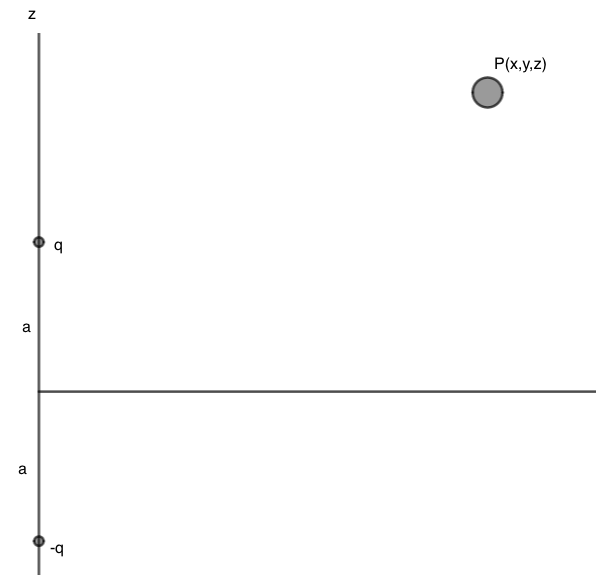
\includegraphics[scale=0.4]{5-3.PNG}}
\end{figure}

\subsubsection{Wangsness 5-4}

$\phi = \frac{1}{4\pi \epsilon_0} \sum \frac{q_i}{R_i} = \frac{1}{4\pi \epsilon_0}\bigg[ \frac{q}{\sqrt{a^2/4}}+\frac{2q}{\sqrt{a^2/2}}-\frac{4q}{\sqrt{a^2/2}}+\frac{3q}{\sqrt{a^2/2}}\bigg] = \frac{q}{\sqrt{2}\pi \epsilon_0 a}$. To know $\B{E}$ from $\phi$, $\phi$ must be known in some region about the point, not just at the point. To be precise in mathematical terms, we must know $\phi$ in some open set about the point in order to compute $\nabla(\phi)$. This is analogous to functions in calculus. Suppose $f$ is a function and $a$ is a real number, and suppose we know the value of $f(a)$. Can we determine what $f'(a)$ is? The answer is no, there is not enough information. If we know what $f(x)$ is in some interval $(a-\epsilon,a+\epsilon)$, then we can compute $f'(a)$.
\begin{figure}[!h]
  \centering
  \subfloat[Drawing for 5-4]{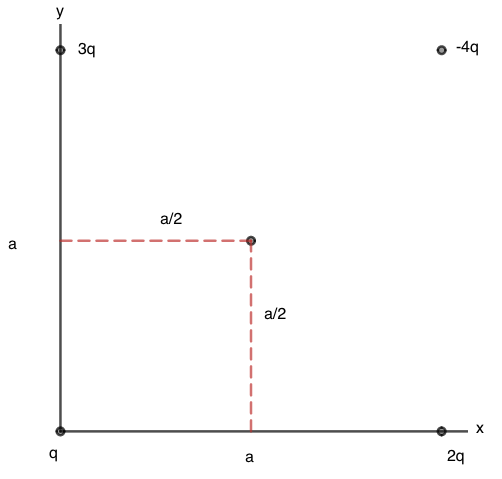
\includegraphics[scale=0.4]{5-4.PNG}}
\end{figure}



\subsubsection{Wangsness 5-10}

We know that $\B{E} = \begin{cases} \frac{2A a^{7/2}}{7\epsilon_0 r^2}\Bh{r}, & r>a \\ \frac{2A r^{3/2}}{7\epsilon_0}, & r<a\end{cases}$. So, $\Delta \phi = \int \B{E} \cdot \B{d\ell}$. Now, $\B{d\ell} = -dr(\Bh{-r}) = \B{dr}$. We split the integral into two parts and compute: $\int \B{E}\cdot \B{d\ell} = \int_{0}^{a} \B{E}\cdot \B{dr} + \int_{a}^{\infty} \B{E}\cdot \B{dr} = \frac{4A a^{5/4}}{35 \epsilon_0}\bigg[ \frac{7}{2}-\big(\frac{r}{a}\big)^{7/2}\bigg]$.

\subsubsection{Wangsness 5-11}

We have that $\B{E} = \begin{cases} \B{0}, & r<a\\ \frac{Q}{4\pi \epsilon_0}\bigg(\frac{r^3-a^3}{b^3-a^3}\bigg)\Bh{r}, & a\leq r \leq b\\ \frac{Q}{4\pi \epsilon_0 r^2}\Bh{r}, & r>b\end{cases}$ We thus split the integral into three regions and compute: $\Delta\phi=\int \B{E}\cdot \B{d\ell} = \int_{0}^{a} \B{E}\cdot \B{dr}+\int_{a}^{b} \B{E}\cdot \B{dr}+\int_{b}^{\infty} \B{E}\cdot \B{dr}$. We then obtain $\phi(\B{r}) = \begin{cases} \frac{\rho_c(b^3-a^3)}{3\epsilon_0 r}, & r>b \\ \frac{\rho}{3\epsilon_0}\bigg[ \frac{3}{2}b^2-\frac{r^2}{2}-\frac{a^3}{r}\bigg], & a\leq r \leq b\\ \frac{\rho_c}{2\epsilon_0}(b^2-a^2), & r<a\end{cases}$

\subsubsection{Wangsness 5-14}

$\phi = \frac{1}{4\pi \epsilon_0}\iint \frac{\sigma_c da'}{R}$. Here, $R = |\B{r}-\B{r}'| = \sqrt{a^2+r^2-2ar\cos(\theta')}$, and $da' = a^2\sin(\theta')d\theta'd\phi'$. So, we have $\phi = \frac{\sigma_c}{4\pi \epsilon_0}\int_{0}^{2\pi}\int_{0}^{\pi} \frac{a^2\sin(\theta')d\theta' d\phi'}{\sqrt{a^2+r^2-2ar\cos(\theta')}} = \frac{\sigma_c a^2}{2\epsilon_0}\int_{0}^{\pi} \frac{\sin(\theta')d\theta'}{\sqrt{a^2-r^2-2ar\cos(\theta')}}$. Let $u = \cos(\theta')$. Then $du = -\sin(\theta')d\theta'$, and we have $-\int\frac{du}{\sqrt{a^2+r^2-2aru}}$. Note that $r$ and $a$ are constants in the integral, and thus this can be computed by trigonometric substitution (Or wolframalpha/integral tables if you're lazy). We thus have $\phi(\B{r}) = \begin{cases}\frac{a^2\sigma}{\epsilon_0 r}, & r>a \\ \frac{a\sigma}{\epsilon_0}, & r<a\end{cases}$.


\subsection*{Homework VII}

\subsubsection{Wangsness 6-6}

Before the connection, $Q=C_1 \Delta \phi$. After the connection, $Q_1 = C_1 \Delta\phi'$, $Q_2 = C_2 \Delta \phi'$, $Q_1+Q_2=Q$, and $Q_1+Q_2=(C_1+C_2)\Delta \phi' = Q = C_1\Delta \phi$. Thus, $\Delta \phi' = \frac{C_1}{C_1+C_2}\Delta \phi$, $Q_1 = \frac{C_1^2}{C_1+C_2}\Delta \phi$, and $Q_2 = \frac{C_1 C_2}{C_1+C_2}\Delta \phi$.

\subsubsection{Wangsness 6-7}
For Parallel:\\
$Q_1 = C_1\Delta \phi$, $Q_2 = C_2\Delta \phi$, where $Q_1$ and $Q_2$ are the charges on the plates $C_1$ and $C_2$, respectively. The total charge is $Q_1+Q_2$. Thus, $Q=Q_1+Q_2 = C_1\Delta\phi + C_2 \Delta \phi =(C_1+C_2)\Delta\phi = C_p \Delta \phi$, where $C_p$ is $C_1+C_2$. \\
For Series:\\
$\Delta \phi = \Delta\phi_1 + \Delta \phi_2$, where $\Delta\phi_1$ and $\Delta \phi_2$ are the potential differences across $C_1$ and $C_2$, respectively. If a charge $Q$ is on the left plate of $C_1$, then there is a charge $-Q$ on the right plate, and therefore there is a charge $Q$ on the left plate of $C_2$ as well. Thus, $Q=Q_1=Q_2$. So, $\Delta \phi = \frac{Q_1}{C_1} + \frac{Q_2}{C_2} = \frac{Q}{C_1}+\frac{Q}{C_2} = Q\big(\frac{1}{C_1}+\frac{1}{C_2}\big) = \frac{Q}{C_s}$, where $\frac{1}{C_s} = \frac{1}{C_1}+\frac{1}{C_2}$.

\subsubsection{Wangsness 6-9}

At $r=a$, $E=\frac{Q}{4\pi \epsilon_0 a^2}$, $Q=C\Delta \phi$, and $C=\frac{4\pi \epsilon_0 ab}{b-a}$. Thus, we may write $E$ as $E=\frac{b\Delta \phi}{a(b-a)}$. To minimize this, we solve $\frac{\partial E}{\partial a} = 0$. This gives us $a=\frac{b}{2}$. To check that is is a minimum, we check $\frac{\partial^2 E}{\partial a^2}\bigg|_{a=\frac{b}{2}}$. This gives us $\frac{32\Delta \phi}{b}$, which is positive. Therefore $a=\frac{b}{2}$ is a minimum.

\subsubsection{Wangsness 6-10}

$E=\frac{\lambda}{2\pi \epsilon_0 \rho}$, where $\lambda$ is the linear charge density, $\lambda = \frac{Q}{L}$. Thus, $\Delta\phi = - \int_{b}^{a} \frac{\lambda}{2\pi \epsilon_0\rho}d\rho = \frac{\lambda}{2\pi \epsilon_0}\ln\big(\frac{b}{a}\big)$. We have that $C=\frac{Q}{\Delta\phi}$, and thus $C = \frac{2\pi \epsilon_0 L}{\ln\big(\frac{b}{a}\big)}$


\subsection*{Homework VIII}

\subsubsection{Wangsness 7-2}

$U_e = \underset{All\ Pairs}\sum\frac{q_i q_j}{r\pi \epsilon_0 R_{ij}}$, where $R_{ij} = |\B{r}_i-\B{r}_j| = \sqrt{r_i^2+r_j^2 -2\B{r}_i\cdot \B{r}_j}$. Computing the sum, we get $U_e = \frac{q^2}{4\pi \epsilon_0 a}\big(12 + \frac{12}{\sqrt{2}}+\frac{4}{\sqrt{3}}\big)$.

\begin{figure}[!h]
  \centering
  \subfloat[Drawing for 7-2]{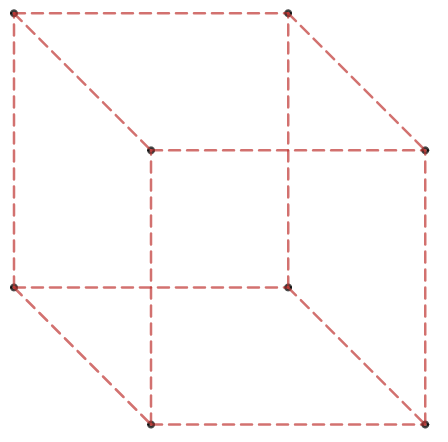
\includegraphics[scale=0.4]{7-2.PNG}}
\end{figure}

\subsubsection{Wangsness 7-4}

$\rho_c = Ar^n$, where $A$ is a constant and $n\geq 0$. Thus, $U_e = \frac{1}{2} \int \rho_c(\B{r})\phi(\B{r})d\tau$. We have that $E = \frac{Aa^{n+3}}{\epsilon_0 (n+3)r^2}$ for $r\geq a$, and $E=\frac{Ar^{n+1}}{\epsilon_0(n+3)}$ for $r\leq a$ from Gauss' Law. Now, all of the charges are located within $r\leq a$, and so we must compute $\phi$ in this region. Letting $\phi(r)\rightarrow 0$ as $r\rightarrow \infty$, we may compute $\phi$ as $\phi(r) = -\int_{\infty}^{r}\B{E}\cdot \B{d\ell} = -\int_{\infty}^{a} \B{E}\cdot \B{d\ell} - \int_{a}^{r}\B{E}\cdot \B{d\ell} = \frac{Aa^{n+3}}{\epsilon_0(n+3)a}+\frac{Aa^{n+2}}{\epsilon_0(n+2(n+3)}-\frac{Ar^{n+2}}{\epsilon_0(n+3)(n+2)}$. We can now compute  the potential energy. $U_e =\frac{1}{2}\int \rho_c(\B{r})\phi(\B{r})d\tau = \int_{0}^{2\pi} \int_{0}^{\pi}\int_{0}^{a} A r^n \bigg(\frac{Aa^{n+3}}{\epsilon_0(n+3)a}+\frac{Aa^{n+2}}{\epsilon_0(n+2)(n+3)}-\frac{Ar^{n+2}}{\epsilon_0(n+3)(n+2)}\bigg)r^2 \sin(\theta)dr d\theta d\phi = \frac{2\pi A^2}{\epsilon_0 (n+3)}\bigg[\frac{a^{2n+5}}{n+3}+\frac{a^{2n+5}}{(n+2)(n+3)}-\frac{a^{2n+5}}{(n+2)(2n+5)}\bigg]$. Taking the limit as $n\rightarrow 0$, we get $\frac{3}{5}\bigg[\frac{Q^2}{4\pi \epsilon_0 a}\bigg]$, as expected for a constant spherical charge density.

\subsubsection{Wangsness 7-6}

\begin{figure}[!h]
  \centering
  \subfloat[Drawing for 7-6]{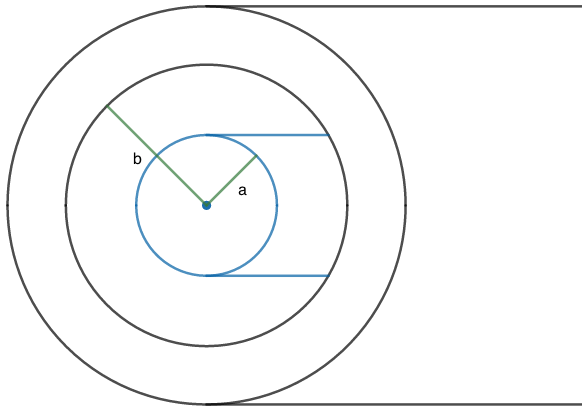
\includegraphics[scale=0.4]{7-6.PNG}}
\end{figure}

$U_e = \frac{1}{2}\int_{S}\sigma_c(\B{r})\phi(\B{r})da$. In the region between the cylinders we have that $E = \frac{\lambda}{2\pi \epsilon_0 \rho}$, and thus $\phi= \frac{\lambda 2\pi \epsilon_0}\ln\big(\frac{\rho_0}{\rho}\big)$, where $\rho_0$ is the zero of $\phi$. We can now compute $U_e$ and we get $U_e = \frac{\lambda L}{4\pi \epsilon_0}\ln\big(\frac{b}{a}\big)$. As $U_e = \frac{1}{2}\frac{Q^2}{C}$, we get $C= \frac{2\pi \epsilon_0 L}{\ln\big(\frac{b}{a}\big)}$

\subsubsection{Wangsness 7-9}

The electric field is $\B{E}_i = \frac{Qr}{4\pi \epsilon_0 a^3}\Bh{r}$ inside the distribution, and $\B{E}_o = \frac{Q}{4\pi\epsilon_0r^2}\Bh{r}$. The energy density inside is thus $\mu_{e_i} = \frac{1}{2}\epsilon_0 E_i^2=\frac{Q^2r^2}{32\pi^2 \epsilon_0 a^6}$ and outside is $\mu_{e_o} = \frac{1}{2}\epsilon_0 E_0^2 = \frac{Q^2}{32\pi^2 \epsilon_0 r^4}$. The total energy is $\int_{Inside} \mu_{e_i}d\tau + \int_{Outside} \mu_{e_o}d\tau$. Computing this integral, we get $U_e = \frac{3}{5}\bigg( \frac{Q^2}{4\pi \epsilon_0}\bigg)$, in agreement with before.

\subsubsection{Wangsness 7-10}

$U_e = \frac{\epsilon_0}{2} \underset{All\ Space}\int E^2 d\tau$. The $\B{E}-$Field in between the spheres is $\frac{Q}{4\pi \epsilon_0 r^2}\Bh{r}$. The energy associated to this region is thus $\int_{0}^{2\pi}\int_{0}^{\pi}\int_{a}^{b} \frac{\epsilon}{2} \frac{Q^2}{16\pi^2 \epsilon_0^2 r^4}r^2\sin(\theta) dr d\theta d\phi = \frac{Q^2}{8\pi \epsilon_0}\bigg(\frac{b-a}{ab}\bigg)$. We have that $C = \frac{1}{2} \frac{Q^2}{U_e}$, and thus $C = \frac{4\pi \epsilon_0 ab}{b-a}$.

\subsubsection{Wangsness 7-17}

$\B{E} = \frac{\lambda}{2\pi \epsilon_0 \rho}\Bh{\rho}$, $\Delta\phi = \frac{\lambda}{2\pi \epsilon_0 \ln\big(\frac{b}{a}\big)}$, and therefore $\lambda = \frac{2\pi \epsilon_0 \Delta\phi}{\ln\big(\frac{b}{a}\big)}$ and $E = \frac{\Delta \phi}{\rho \ln\big(\frac{b}{a}\big)}$. So, $f_e = \mu_e = \frac{1}{2} \epsilon_0 E^2\bigg|_{\rho = a} = \frac{1}{2} \epsilon_0 \bigg[ \frac{\Delta\phi}{a \ln\big(\frac{b}{a}\big)}$. Thus, $\B{F}_{Tot} = \int f_e \B{da} = f_e \int \B{da} = 0$.



\subsection*{Homework IX}

\subsubsection{Wangsness 8-5}

The monopole moment is $Q = \sum q_i = -3q-2q-q+q+2q+3q+4q+5q=9q$.
The dipole moment is $\B{p} = \sum q_i \Bh{r}_i = (-3q)\B{0} + (-2q)a\Bh{x} + (-q)(a\Bh{x}+a\Bh{y})+qa\Bh{y} + 2q(a\Bh{y}+a\Bh{z})+3q(a\Bh{x}+a\Bh{y}+a\Bh{z})+4q(a\Bh{x}+a\Bh{z})+5qa\Bh{z}=4qa\Bh{x}+5qa\Bh{y}+14aq\Bh{z}$

\begin{figure}[!h]
  \centering
  \subfloat[Drawing for 8-5]{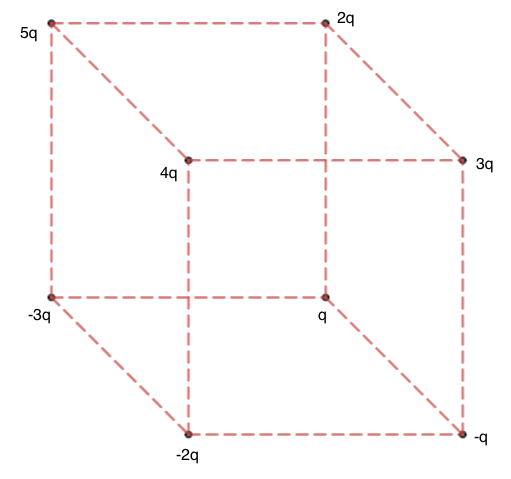
\includegraphics[scale=0.4]{8-5.PNG}}
\end{figure}

It is possible to find an origin about which the dipole moment will vanish. Consider an arbitrary charge distribution with the center of charge designated as c.c. The position vector of this is $\B{r}_{c.c.} = \frac{\int \B{r}' \rho d\tau '}{\int \rho d\tau '} = \frac{\sum \B{r}_i q_i}{\sum q_i}$. Shifting the origin by $\B{r}_{c.c.}$ the dipole moment becomes zero. The original dipole moment is $\B{p}_{o} = \int \B{r}' d\tau ' = \sum \B{r}_i q_i$. The new dipole moment will be $\B{p}_N = \int (\B{r}' - \B{r}_{c.c.})d\tau' = \int \B{r}' d\tau' - \B{r}_{c.c.} \int \rho d\tau' = \sum \B{r}_i q_i - \B{r}_{c.c} \sum q_i = \sum \B{r}_i q_i - \frac{\sum \B{r}_i q_i }{\sum q_i}\sum q_i = \B{0}$. For the problem at hand, this equates to $\B{r}_{c.c} = \langle \frac{4}{9}a, \frac{5}{9}a, \frac{14}{9}a\rangle$ (In Cartesian Coordinates).

\subsubsection{Wangsness 8-8}

$Q = \int_{S'} \sigma da' = \int_{0}^{2\pi} \int_{0}^{\pi} \sigma_{0} \cos(\theta) a^2 \sin(\theta) d\theta d\phi = 2\pi \sigma_{0} \int_{0}^{2\pi} \sin(\theta)\cos(\theta)d\theta = 0$. Thus, $Q=0$. $\B{p} = \int_{S'}\sigma \B{r}' da' = \int_{0}^{2\pi} \int_{0}^{\pi} \sigma \cos(\theta) \big( a\sin(\theta) \cos(\phi) \Bh{x} + a \sin(\theta)\sin(\phi) \Bh{y} + a\cos(\theta) \Bh{z}\big)a^2\sin(\theta)d\theta d\phi = \frac{4\pi \sigma_0 a^3}{3} \Bh{z}$. $\phi \approx \frac{1}{4\pi \epsilon_0} \frac{\B{p}\cdot \Bh{r}}{r^2} = \frac{\sigma_0 a^3}{3\epsilon_0^2 r^2}\cos(\theta)$

\subsubsection{Wangsness 9-1}

Surface of Separation between regions $1$ and $2$ is a plane $f=2x+y+z=1$. $\B{E}_1 = 4\Bh{x}+\Bh{y}-3\Bh{z}$ is given. Find the normal and tangential component of $\B{E}_1$: The unit vector is the normal to the plane which is $\Bh{n}=\frac{\nabla(f)}{|\nabla(f)|} = \frac{2\Bh{x}+\Bh{y}+\Bh{z}}{\sqrt{6}}$. The normal component of $\B{E}_1$ is $\B{E}_1 \cdot \Bh{n} = \sqrt{6}$. Thus, $\B{E}_{1n} = (\B{E}_1 \cdot \Bh{n})\Bh{n} = 2\Bh{x}+\Bh{y}+\Bh{z}$. The tangential component is $\B{E}_1 - \B{E}_{1n} = 2\Bh{x}-4\Bh{z}$.

\subsubsection{Wangsness 9-3}

We are given the density $\sigma = \sigma_0 \cos(\theta) = \frac{\sigma_0 z}{a}$ and $\B{E}_1 = \alpha \Bh{x}+\beta \Bh{y}+ \gamma \Bh{z}$. The boundary conditions are $E_{2t} = E_{1t}$ and $E_{2n}-E_{1n} = \frac{\sigma}{\epsilon_0}$. We can write $\B{E}_1 = E_{1t}\Bh{\mu}+E_{1n} \Bh{r}$ where $\Bh{r}$ is the normal to the spherical surface and $\Bh{\mu}$ is the tangent to the sphere. On the outside, $\B{E}_2 = E_{2t}\Bh{\mu}+E_{2n}\Bh{r}$. Now, using the boundary conditions the $E-$field on the outside is $\B{E}_2 = E_{1t}\Bh{\mu}+(\frac{\sigma}{\epsilon_0}+E_{1n})\Bh{r} = E_{1t}\Bh{\mu}+E_{1n}\Bh{r}+\frac{\sigma}{\epsilon_0}\Bh{r} = \alpha \Bh{x}+\beta \Bh{y}+\gamma \Bh{z} + \frac{\sigma z}{\epsilon_0 a}\bigg(\frac{x\Bh{x}+y\Bh{y}+z\Bh{z}}{a}\bigg)$. So, $\B{E}_2 = \big(\alpha+\frac{\sigma_0 zx}{\epsilon_0 a^2}\big)\Bh{x}+\big(\beta + \frac{\sigma_0 zy}{\epsilon_0 a^2}\big)\Bh{y}+\big(\gamma+ \frac{\sigma_0 z^2}{\epsilon_0 a^2}\big)\Bh{z}$


\subsection*{Homework X}

\subsubsection{Wangsness 10-3}

$\B{P}= P(1+\alpha z)\Bh{z}$, where $P$ and $\alpha$ are constants. Volume charge density is $\rho_{b} = -\nabla \cdot \B{P} = -\alpha P$. The surface charge densities are $\B{P}\cdot \Bh{n}$, so $\sigma_{top} = P(1+\alpha t)$ and $\sigma_{bottom} = -P$. On the left and right sides the charge density is zero as the normals to the sides are at right angles with $\B{P}$. So, $Q = \int_{V} \rho d\tau' + \int_{top} \sigma_{top} da' + \int_{bottom} \sigma_{bottom} da' = \int_{V}-\alpha P d\tau' + \int_{top}P(1+\alpha t) da' + \int_{bottom} - Pda' = \alpha PAt + PA - \alpha PA t - PA = 0$
\begin{figure}[!h]
  \centering
  \subfloat[Drawing for 10-3]{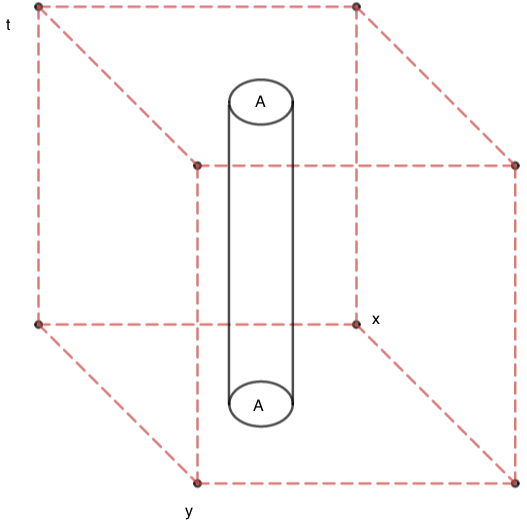
\includegraphics[scale=0.4]{10-3.PNG}}
\end{figure}

\subsubsection{Wangsness 10-6}

We are given that $\B{P} = P_0 \Bh{k}$. Now $\rho_{b} = -\nabla \cdot \B{P}$, and as $\B{P}$ is uniform, $-\nabla \cdot \B{P} = 0$. Thus $\rho_b = 0$. $\sigma_b = \B{P}\cdot \Bh{n} = P_0 \Bh{k} \cdot \Bh{n} = P_0 \cos(\theta)$. The positive charge is thus located in the region $\theta < \frac{\pi}{2}$. So $Q_b^+ = \int_{0}^{\pi/2}\int_{0}^{2\pi} P_0 \cos(\theta) a^2 \sin(\theta) d\theta d\phi = \pi a^2 P_0$.

\begin{figure}[!h]
  \centering
  \subfloat[Drawing for 10-6]{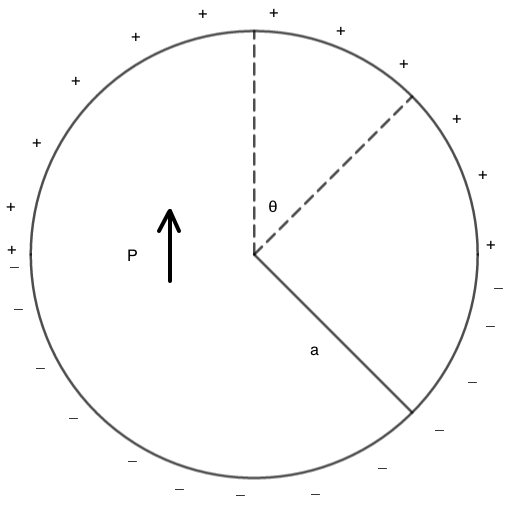
\includegraphics[scale=0.3]{10-6.PNG}}
\end{figure}

\subsubsection{Wangsness 10-17}

Choose a spherical Gaussian surface outside the sphere concentric with the given sphere. $\int \B{D}\cdot \B{da} = Q_f$, so $D_o (4\pi r^2) = q$, and thus $\B{D}_o = \frac{q}{4\pi r^2} \Bh{r}$. From $\B{D} = \epsilon_0 \B{E}+\B{P}$, we have that $\B{D}_o - \epsilon_0 \B{E}_o = \B{P}_o$. $\B{E}_0 = \frac{q}{4\pi \epsilon_0 r^2}\Bh{r}$, and thus $\B{P}_o = 0$. There is no dielectric outside of the sphere. Choosing a Gaussian surface inside of the sphere, we get $\int \B{D}\cdot \B{da} = Q_f$, for $D(4\pi r^2) = q$, and thus $\B{D}_i = \frac{q}{4\pi r^2} \Bh{r}$. $\B{E}_i = \frac{\B{D}_i}{\epsilon} = \frac{\B{D}_i}{\kappa_e \epsilon_0} = \frac{q}{4\pi \kappa_{e} \epsilon_0 r^2}\Bh{r}$. So $\B{P}_i = \B{D}_i - \epsilon_0 \B{E}_i = (1-\frac{1}{\kappa_{e}}) \frac{q}{4\pi r^2} \Bh{r}$. Finally, $Q_b^{surface} = \int_{S} \sigma_{b} da' = \iint \B{P}\cdot \Bh{n} da' = \int_{0}^{\pi} \int_{0}^{2\pi} \frac{\kappa_e-1}{\kappa_e} \frac{q}{4\pi} \sin(\theta) d\theta d\phi = \frac{\kappa_e-1}{\kappa_e} q$.

\subsubsection{Wangsness 10-18}

$\oint \B{D} \cdot \B{da} = q$. $\B{D} = \frac{q}{4\pi r^2} \Bh{r}$ for all $r$ inside the cavity or in the dielectric. $\rho_b = 0$ since $\rho_f = 0$ in the dielectric. In the dielectric $\B{E} = \frac{\B{D}}{\epsilon} = \frac{\B{D}}{\kappa_e \epsilon_0}$, so $\B{E} = \frac{q}{4\pi \kappa_e \epsilon_0 r^2}\Bh{r}$. $\B{P} = \B{D}- \epsilon_0 \B{E} = \frac{\kappa_e-1}{\kappa_e} \frac{q}{4\pi r^2} \Bh{r}$ at the surface of the cavity $r=a$. $\sigma_b = \B{P}\cdot \Bh{n} = \frac{\kappa_e-1}{\kappa_e} \frac{q}{4\pi a^2} \Bh{r}\cdot (-\Bh{r}) = - \frac{\kappa_e-1}{\kappa_e} \frac{q}{4\pi a^2}$. $Q_b^{cavity} = \int \sigma da = - \frac{\kappa_e-1}{\kappa_e}q$.

\subsubsection{Wangsness 10-25}

$\kappa_e(x) = \alpha+\beta x$ (The dielectric constant varies linearly with $x$. $\alpha$ and $\beta$ are constants). Find $\B{D}$ between the plates. $\int_{Gaussian Surface} \B{D}\cdot \B{da} = Q_f^{enc}$ (D is uniform between plates). $D\Delta a = Q_f^{enc}$, and thus $D = \frac{Q_f^{enc}}{\Delta a} = \sigma = \frac{Q}{A}$, where $Q$ is the total charge of the plate and $A$ is the area of the plate. $E = \frac{D}{\epsilon} = \frac{Q}{\kappa \epsilon_0 A} = \frac{Q}{\epsilon_0 A(\alpha + \beta x)}$. At $x=0$, $\kappa_e = \kappa_{e_1}$, so $\alpha+\beta(0) = \kappa_{e_1}$, and thus $\alpha = \kappa_{e_1}$. At $x=d$, $\kappa_{e} = \kappa_{e_2}$, and so $\beta = \frac{\kappa_{e_2}-\kappa_{e_1}}{d}$. The potential difference between the plates is $\Delta \phi = -\int_{-}^{+} \B{E}\cdot \B{d\ell} = \int_{+}^{-} Edx = \frac{Q}{\epsilon_0 A} \int_{0}^{d} \frac{dx}{\alpha+\beta x} = \frac{Q}{\epsilon A} \frac{1}{\beta} \ln(\alpha+\beta x)\big|_{0}^{d} = \frac{Q}{\epsilon_0 A\beta} \ln(\frac{\alpha+\beta d}{\alpha}) = \frac{Q}{\epsilon_0 A\beta} \ln(\frac{\kappa_{e_2}}{\kappa_{e_1}}) = \frac{Q}{C}$. Hence $C = \frac{\epsilon_0 A\beta}{\ln(\frac{\kappa_{e_2}}{\kappa_{e_1}})} = \frac{(\kappa_{e_2}-\kappa_{e_1})\epsilon_0 A}{d\ln(\frac{\kappa_{e_2}}{\kappa_{e_1}})}$

\begin{figure}[!h]
  \centering
  \subfloat[Drawing for 10-25]{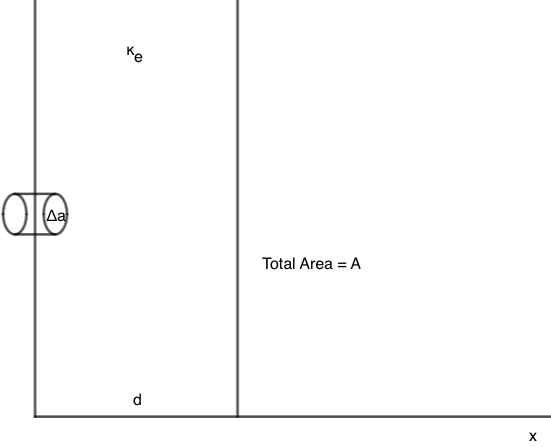
\includegraphics[scale=0.4]{10-25.PNG}}
  \hfill
    \centering
  \subfloat[Drawing for 12-3]{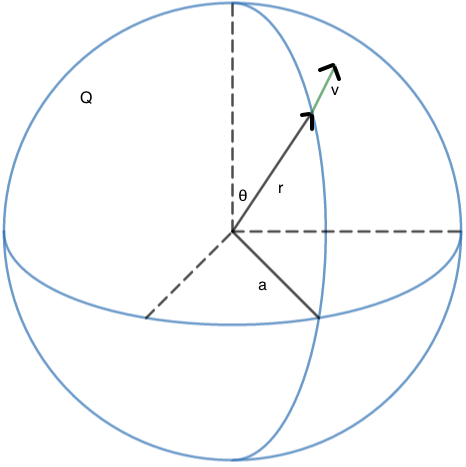
\includegraphics[scale=0.4]{12-3.PNG}}
\end{figure}


\subsubsection{Wangsness 10-27}
$\kappa = \kappa_{e_1}$ for $a\leq \rho < \rho_0$, $\kappa = \kappa_{e_2}$ for $\rho_0 \leq \rho \leq b$. First get $D$ by assuming a charge per unit length $\lambda $on the inner cylinder and $-\lambda$ on the outer. $\int \B{D}\cdot \B{da} = Q_{f}^{enc} = D(2\pi \rho L) = \lambda L$. So $\B{D} = \frac{\lambda}{2\pi \rho} \Bh{\rho}$. $\Delta \phi = -\int_{-}^{+} \B{E} \cdot \B{d\ell} = \int_{a}^{b} \frac{\lambda}{2\pi \rho \epsilon}d\rho = \int_{a}^{\rho_0} \frac{\lambda}{2\pi \epsilon_0 \kappa_{e_1}\rho}d\rho + \int_{\rho_0}^{b} \frac{\lambda}{2\pi \epsilon_0 \kappa_{e_2}\rho}d\rho = \frac{\lambda}{2\pi \epsilon_0}\big[\frac{1}{\kappa_{e_1}}\ln(\frac{\rho_0}{a}) + \frac{1}{\kappa_{e_2}}\ln(\frac{b}{\rho_0})\big]$. From $\Delta \phi = \frac{Q}{C}$, and $Q=\lambda L$, we get $C = \frac{2\pi \epsilon_0 L}{\frac{1}{\kappa_{e_1}}\ln(\frac{\rho_0}{a}) + \frac{1}{\kappa_{e_2}}\ln(\frac{b}{\rho_0})}$


\subsection*{Homework XI}

\subsubsection{Wangsness 12-3}

$\B{J} = \rho \B{v}$. $\rho = \frac{Q}{\frac{4}{3}\pi a^3} = \frac{3q}{4\pi a^3}$. $\B{u} = \B{\omega}\times\B{r} = \omega \Bh{z} \times r \Bh{r} = \omega r \sin(\theta) \Bh{\phi}$. So, we have that $\B{J} = \frac{3Q}{4\pi a^3} \omega r \sin(\theta) \Bh{\phi}$. $\B{da} = rdrd\theta \Bh{\phi}$, so $I = \int \B{J} \cdot \B{da} = \frac{3Q \omega}{4\pi a^3} \int_{0}^{\pi} \int_{0}^{a} r^2\sin(\theta)drd\theta = \frac{Q\omega}{2\pi}$ 

\subsubsection{Wangsness 13-4}

We will calculate the force exerted by $C'$ on $C$. $\B{F}_{C'\rightarrow C} = \frac{\mu_0}{4\pi} \oint_{C} \oint_{C'} \frac{I \B{d\ell}\times (I' \B{d\ell}'\times \Bh{R})}{R^2}$. We use the $BAC-CAB$ rule: $\B{A}\times(\B{B}\times \B{C}) = \B{B}(\B{A}\cdot \B{C}) - \B{C}(\B{A}\cdot \B{B})$. We can rewrite the previous integral as  $\B{F}_{C'\rightarrow C} = -\frac{\mu_0 II'}{4\pi} \oint_{C} \oint_{C'} \big[ \B{d\ell}'\cdot(\B{d\ell}\times \frac{\Bh{R}}{R^2}) - \frac{\Bh{R}}{R^2} \B{d\ell}\cdot \B{d\ell}\big]$. Recall that $\nabla(\frac{1}{R}) = \frac{\Bh{R}}{R^2}$. Using this, we have $\B{F}_{C'\rightarrow C} = -\frac{\mu_0 II'}{4\pi} \oint_{C}\oint_{C'} \B{d\ell'}\big[ \B{d\ell}\cdot \nabla(\frac{1}{R})- \frac{\Bh{R}}{R^2} \B{d\ell'} \cdot \B{d\ell}\big]$. From the fundamental theorem of gradients, $\oint \nabla(f) \cdot \B{d\ell} = 0$ for any function $f$. Thus $\oint \nabla(\frac{1}{R}) \cdot \B{d\ell} = 0$. From this we have $\B{F}_{C\rightarrow C'} = -\frac{\mu_0 II'}{4\pi} \oint_{C}\oint_{C'} \frac{\Bh{R}}{R^2} \B{d\ell}'\cdot \B{d\ell}$. We now compute this integral along all four paths of the problem. $\B{d\ell}' = dz' \Bh{z}$ for all paths. Along path $I$, $\B{r} = \Bh{x}d+\Bh{z}z$, $\B{d\ell} = \Bh{z}dz$. Along path $III$, $\B{r} = \Bh{x}(a+d)+\Bh{z}z$, $\B{d\ell} = \Bh{z}dz$. Along paths $II$ and $IV$, $\B{d\ell}\cdot \B{d\ell}' = 0$. Piecing this together, $\B{F}_{C\rightarrow C'} = -\frac{\mu_0 II'}{4\pi}\int_{0}^{b} \int_{-\infty}^{\infty} \frac{\Bh{x}d+\Bh{z}(z-z')}{\big(d^2+(z-z')^2\big)^{3/2}}dz'dz - \frac{\mu_0 II'}{4\pi} \int_{b}^{0} \int_{-\infty}^{\infty} \frac{\Bh{x}(d+a)+\Bh{z}(z-z')}{\big((d+a)^2+(z-z')^2\big)^{3/2}}dz'dz$. Making the substitution $t=z'-z$, we get an integral of the form $\int_{-\infty}^{\infty} \frac{t+z'}{(A+t^2)^{3/2}}dt$. This is an odd function that is integrated over symmetric bounds, and thus the integral is zero. The only part left is the $\Bh{x}$ contribution. Evaluating this integral, we get $\B{F}_{C\rightarrow C'} = -\frac{\mu_0 II' ab}{2\pi d(a+d)}\Bh{x}$.

\begin{figure}[!h]
  \centering
  \subfloat[Drawing for 13-4]{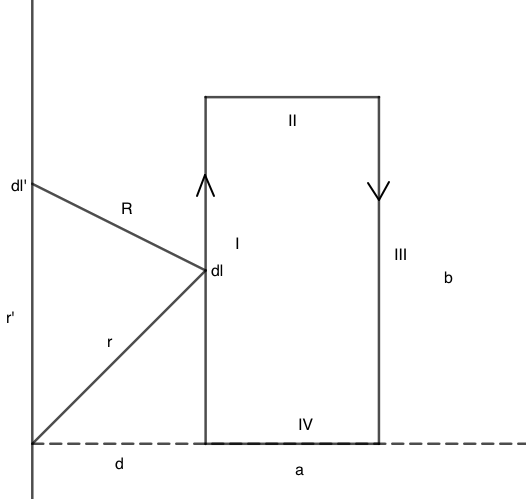
\includegraphics[scale=0.4]{13-4.PNG}}
\end{figure}

\subsubsection{Wangsness 14-7}

$\B{R} = \B{r}-\B{r}'$, where $\B{r} = z\Bh{z}$ and $\B{r}' = a\cos(\phi')\Bh{x}+a\sin(\phi')\Bh{y}$. $\B{d\ell}' = ad\phi' \Bh{\phi}$. Putting this together, we have $\B{R} = z\Bh{z} - a(\cos(\phi')\Bh{x}+\sin(\phi')\Bh{y})$. $\B{B} = \frac{\mu_0 I'}{4\pi}\int \frac{\Bh{d\ell}\times \B{R}}{R^3} = \frac{\mu_0I'}{4\pi} \int_{-\alpha}^{\alpha} \frac{ad\phi' \Bh{\phi}\times (z\Bh{z}-a\cos(\phi')\Bh{x}-a\sin(\phi')\Bh{y})}{(z^2+a^2)^{3/2}}$. $\Bh{\phi} = -\sin(\phi')\Bh{x}+\cos(\phi')\Bh{y}$. So, we have $\frac{\mu_0 I'a}{4\pi(z^2+a^2)^{3/2}}\int_{-\alpha}^{\alpha} (-\sin(\phi')\Bh{x}+\cos(\phi')\Bh{y})\times (-a\cos(\phi')\Bh{x}-a\sin(\phi')\Bh{y}+z\Bh{z})d\phi'$. This simplifies to the integral $\frac{\mu_0 I'a}{4\pi (z^2+a^2)^{3/2}}\int_{-\alpha}^{\alpha} (z\cos(\phi')\Bh{x}+z\sin(\phi')\Bh{y}+a\Bh{z})d\phi'$. Sine is an odd function, and the limit is over a symmetric interval, and thus the $\Bh{y}$ component is zero. The final integral is $\frac{\mu_0 I' a}{2\pi (z^2+a^2)^{3/2}}\big(z\sin(\alpha)\Bh{x}+a\alpha \Bh{z}\big)$

\subsubsection{Wangsness 14-15}

The force on $q$ is given by $\B{F} = q\B{v}\times \B{B}$. We first get $\B{B}$ at $q$. $\B{B} = \frac{\mu_0}{4\pi} \int \frac{I' d\ell' \times \Bh{R}}{R^2}$. For this problem, $\B{R} = -\rho' \Bh{\rho}$. We need only compute the integral along paths $I$ and $III$, for along $II$ and $IV$ we have that $\B{d\ell}$ and $\B{R}$ are parallel. So, we have $\B{B} = \frac{\mu_0}{4\pi} \int_{0}^{\pi} \frac{I'(-ad\phi' \Bh{\phi})\times (-a\Bh{\rho})}{a^3}+ \frac{\mu_0}{4\pi} \int_{0}^{\pi} \frac{I'(bd\phi' \Bh{\phi})\times (-b\Bh{\rho})}{b^3} = \frac{\mu_0 I'}{4} \frac{b-a}{ab} \Bh{z}$. The force is $\B{F} = qv\Bh{y} \times \frac{\mu_0 I}{4} \frac{b-a}{ab} \Bh{z} = \frac{qv\mu_0 I'}{4} \frac{b-a}{ab} \Bh{x}$

\begin{figure}[!h]
  \centering
  \subfloat[Drawing for 14-15]{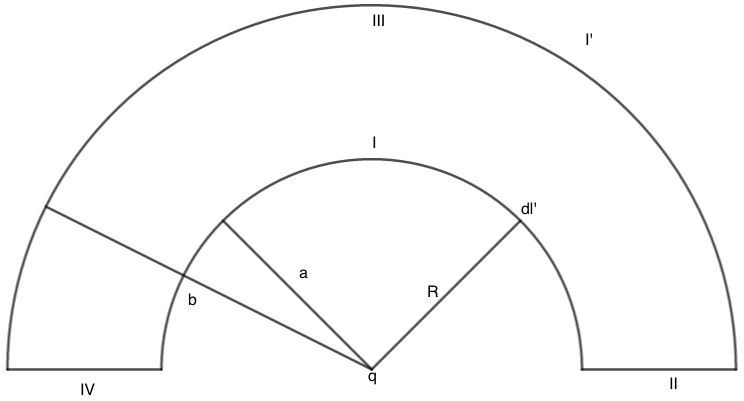
\includegraphics[scale=0.4]{14-15.PNG}}
\end{figure}


\subsection*{Homework XII}

\subsubsection{Wangsness 15-7}

For $\rho\leq a$, path $(1)$ has $\oint \B{B}\cdot \B{d\ell}= \mu_0 I_{enc}$, where $I_{enc} = I\frac{\rho^2}{a^2}$. So $\B{B} = \frac{\mu_0 I\rho}{2\pi a^2} \Bh{\phi}$. For $a\leq \rho \leq b$, $I_{enc} = I$. So $B = \frac{\mu_0 I}{2\pi \rho} \Bh{\phi}$. For $b\leq \rho \leq c$, $I_{enc} = I =I\frac{\rho^2-b^2}{c^2-b^2} = I\frac{c^2-\rho^2}{c^2-b^2}$. So $\B{B} = \frac{\mu_0 I}{2\pi \rho} \frac{c^2-\rho^2}{c^2-b^2}\Bh{\phi}$. FInally, or $\rho \geq c$, $I_{enc} = 0$, so $\B{B} = 0$.

\begin{figure}[!h]
  \centering
  \subfloat[Drawing for 15-7]{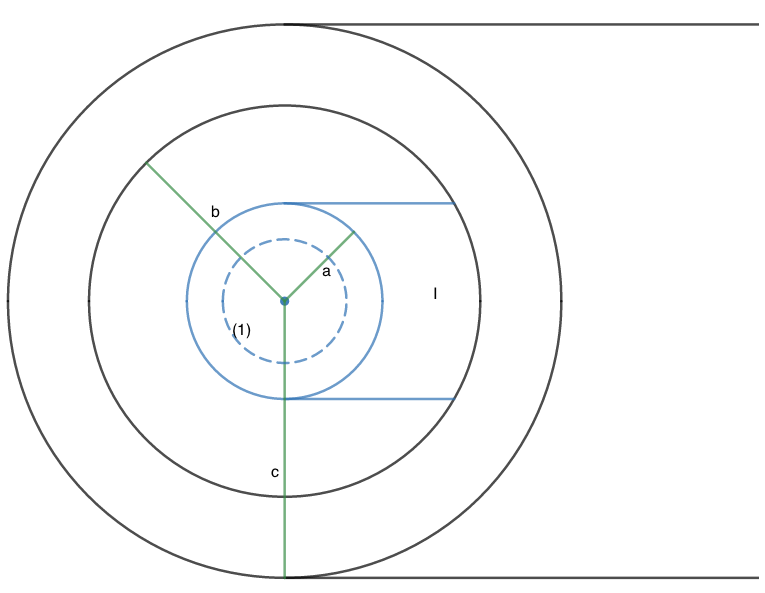
\includegraphics[scale=0.4]{15-7.PNG}}
\end{figure}


\subsubsection{Wangsness 15-8}

$\B{B} = \begin{cases} 0, & \rho < a \\ \frac{\mu_0 I}{2\pi \rho}\frac{\rho^2-a^2}{b^2-a^2}\Bh{\phi}, & a<\rho < b \\ \frac{\mu_0 I}{2\pi \rho} \Bh{\phi}, & \rho>b\end{cases}$. By definition, $\mu_0 \B{J} = \nabla \times \B{B}$. So, $\B{J} = \begin{cases} 0, & \rho<a\\ \frac{I}{\pi(b^2-a^2)}, a<\rho < b\\ 0, & \rho>b \end{cases}$. The current $I$ i distributed uniformly over the volume between two coaxial cylinders of inner radius $a$ and outer radius $b$ in the direction of the cylinder axis.

\subsubsection{Wangsness 16-10}

The field point is on the $z-$axis. $\B{r} = z\Bh{z}$, $\B{r}' =  a\cos(\phi')\Bh{x}+a\sin(\phi')\Bh{y}$. $\B{d\ell}' = \B{dr}' = ad\phi' \Bh{\phi} = ad\phi' (-\sin(\phi')\Bh{x}+\cos(\phi')\Bh{y})$. $\B{A} = \frac{\mu_0 I'}{4\pi} \int \frac{\B{d\ell}'}{R} = \frac{\mu_0 I'}{4\pi} \frac{a}{\sqrt{a^2+z^2}}\int_{-\alpha}^{\alpha} (-\sin(\phi')\Bh{x}+\cos(\phi')\Bh{y})d\phi' = \frac{\mu_0 I'a}{2\pi \sqrt{a^2+z^2}}\sin(\alpha)\Bh{y}$. To find $\B{B}$ from $\B{A}$, we need to evaluate $\nabla \times \B{A}$. We don't know about $\B{A}$ for a general point, and thus we can't evaluate the $x$ and $y$ derivatives.



\subsection*{Homework XIII}

\subsubsection{Wangsness 17-3}

The $\B{B}$ field associated with $I$ is $\B{B} = \frac{\mu_0 I}{2\pi \rho} \Bh{\phi}$. In the plane of the paper, $\phi$ is into the paper. $\Phi = \int \B{B}\cdot \B{da} = \int \frac{\mu_0 I}{2\pi \rho} \cdot b d\rho \Bh{\phi} = \frac{\mu_0Ib}{2\pi} \int_{d}^{d+a} \frac{d\rho}{\rho}= \frac{\mu_0 Ib}{2\pi} \ln(\frac{d+a}{d}) = \frac{\mu_0 bI_0 e^{-\lambda t}}{2\pi} \ln(\frac{d+a}{d}) = \frac{\mu_0 I_0 \lambda b}{2\pi} \ln(\frac{d+a}{d})e^{-\lambda t}$. The induced current is clockwise around the loop to produce a field which goes into the paper to counteract the decreasing $\B{B}$ due to $I_0$.

\subsubsection{Wangsness 17-4}

The $\B{B}-$field at distance $\rho$ from the wire at points in the plane of the paper is $\B{B} = \frac{\mu_0 I}{2\pi \rho} \Bh{y}$. The flux of $\B{B}$ through the loop is $\Phi = \int \B{B}\cdot \B{da} = \iint \frac{\mu_0 I}{2\pi \rho}\rho d\theta d\rho$. We have $\rho = b+r\cos(\theta)$. So $\Phi = \frac{\mu_0 I}{2\pi} \int_{0}^{a} \int_{0}^{2\pi} \frac{r d\theta dr}{b+r\cos(\theta)} = \frac{\mu_0 I}{2\pi} \int_{0}^{a} \frac{2r}{\sqrt{b^2-r^2}}\tan^{-1}\big[\frac{\sqrt{b^2-r^2}\tan(\theta/2)}{b+r}\big]_{0}^{2\pi} \Rightarrow \tan^{-1}\big[\frac{\sqrt{b^2-r^2}}{b+r}\tan(\pi)\big] - \tan^{-1}\big[ \frac{\sqrt{b^2-r^2}}{b+r}\tan(0)\big]$. So $\Phi = \mu_0 I\big[b-\sqrt{b^2-a^2}\big]$. The loop moves with constant speed $v$ along the $x-$axis away from the current $I$, $v = \frac{db}{dt}$. So $\xi = -\frac{d\Phi}{dt} = -\mu_0 I \frac{d}{dt}\big[b-\sqrt{b^2-a^2}\big] = -\mu_0 I\big[ v-\frac{bv}{\sqrt{b^2-a^2}}\big] = \mu_0 NIv\big[ \frac{b}{\sqrt{b^2-a^2}}-1\big]$. The current will be clockwise trying to increase the flux which is decreasing due to motion away from the wire.

\begin{figure}[!h]
  \centering
  \subfloat[Drawing for 17-4]{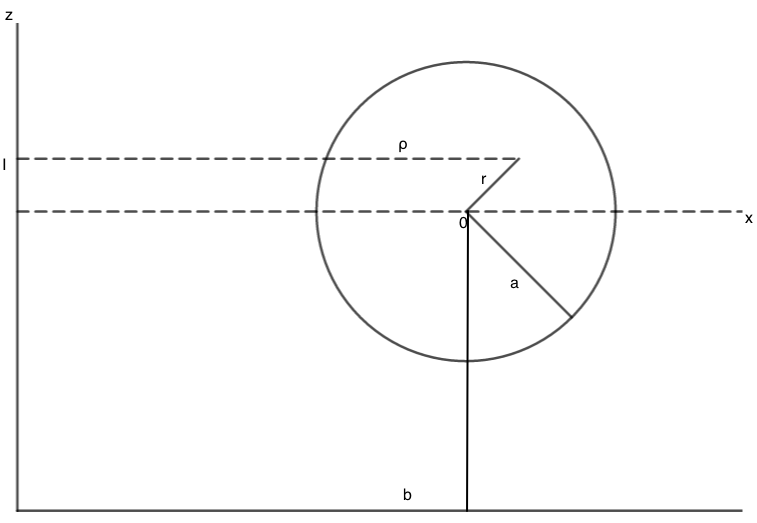
\includegraphics[scale=0.4]{17-4.PNG}}
\end{figure}

\subsubsection{Wangsness 17-19}

$\Phi_{12} = IM_{12}$. The flux due to $1$ through $2$ is $\Phi_{12} = \int \B{B}_1 \cdot \B{da}_2$. $\B{B}_1 = \frac{\mu_0 I}{2\pi} \big( \frac{1}{\rho+d}- \frac{1}{\rho+d+D}\big)$. So we have that $\Phi_{12} = \int_{0}^{a} \frac{\mu_0 I}{2\pi} \big(\frac{1}{\rho+d}- \frac{1}{\rho+d+D}\big) bd\rho = \frac{\mu_0 Ib}{2\pi}\big[ \ln(\frac{a+d}{a+d+D}) - \ln(\frac{d}{d+D})\big]$. Thus, we have $M = \frac{\mu_0 b}{2\pi} \ln\big(\frac{a+d}{d}\big)$

\subsubsection{Wangsness 17-20}

The field inside the toroid is $\B{B} = \frac{\mu_0 NI}{2\pi \rho} \Bh{\phi}$. The flux through a single turn is $\Phi^1 = \frac{\mu_0 NI}{2\pi} \int_{0}^{a} \int_{0}^{2\pi} \frac{r}{b+r\cos(\theta)}d\theta dr$. We've done this integral before, and we get $\Phi^1= \mu_0 NI\big[b-\sqrt{b^2-r^2}\big]$. $\Phi = N\Phi^1$. $L = \frac{\Phi}{I} = \frac{\mu_0 N^2 I}{I} \big[b-\sqrt{b^2-r^2}\big] = \mu_0 N^2 \big[b-\sqrt{b^2-r^2}\big]$

\section{Exams}

\subsection*{Exam I}

\subsubsection{Question I}

Give the vector field field $\B{A} = c\Bh{\theta}$, where $c$ is a constant, find $\nabla \times \B{A}$. Is this a conservative vector field? Explain.

\subsubsection{Question II}

Verify the Divergence Theorem for $\B{A}$ given in problem 1 in spherical coordinates for a hemisphere of radius $a_0$ resting on the $xy-plane$ with the center of the flat base of the hemisphere at the origin and the symmetry axis of the hemisphere along the positive $z-axis$.

\subsubsection{Question III}

A semicircular charged line of radius $a$ carries uniform linear charge density $\lambda$. It has the equation $x^2+y^2 = a^2$, $x\geq 0$, $z=0$. That is, the half circle resting on the $xy-plane$ of radius $a$. Find the electring field at a point $P$ on the $z$ axis a distance $z$ from the origin.

\subsection*{Exam II}


\subsubsection{Question I}
A conducting sphere of radius $a$, centered at the origin carries charge $Q_1$. This sphere is surrounded by a hollow concentric conducting spherical shell of inner radius $b$ and outer radius $c$ with $a<b<c$. The outer hollow conducting shell caries a total charge $Q_2$. 
\begin{enumerate}
\item What is the electric field everywhere?
\item What is the potential everywhere, assuming $\underset{r\rightarrow \infty} \lim \phi(r) = 0$?
\item How much charge is on the inner and outer surfaces of the conducting shell at $r=b$ and $r=c$?
\end{enumerate}

\subsubsection{Question II}
The outer conductor of problem I is now grounded.
\begin{enumerate}
\item What is the electric field everywhere?
\item What is the potential everywhere?
\item How much charge is on the surfaces at $r=b$ and $r=c$?
\item What is the capacitance of the system of conductors?
\item Calculate the electrostatic potential energy of the configuration assuming the energy resides in the charges.
\item Calculate the electrostatic potential energy of the configuration assuming the energy resides in the electric field.
\end{enumerate}

\subsubsection{Question III}
A semicircular arc of radius $a$ in the $y-z$ plane with center on the $y-axis$ at the origin and the top of the arc on the positive $y-axis$ carries linear charge density $\lambda = \lambda_0 \cos(\theta')$, where $\lambda_0$ is constant and $\theta'$ is measured with respected to the positive $z-axis$.
\begin{enumerate}
\item What is the electric monopole moment of this distribution?
\item What is the electric dipole moment of this distribution?
\item What is the electric potential at a distance $r$ from the origin for this distribution where $r>a$, accurate to order $\frac{1}{r^2}$?
\end{enumerate}

\subsection*{Exam III}

\subsubsection{Question I}
The electric field in a spherical region of space of radius $a$ is given by $\B{E} = E_0 \frac{r^2}{a^2}\Bh{r}$ for $r< a$, where $E_0$ is a constant. This region is surrounded concentrically by a grounded conducting spherical shell of inner radius $b$ and outer radius $c$ with $a<b<c$. There is no charge in the region $a<r<b$. 
\begin{enumerate}
\item What is the electric charge density in the region $r<a$?
\item Wher is the electric field in the region $a<r<b$?
\item How much charge is on the surfaces at $r=b$ and $r=c$?
\item What is the electric field for $r>c$?
\item What is the electric potential $\phi$ at $r=0$ assuming that ground potential is $\phi = 0$.
\end{enumerate}

\subsubsection{Question II}
A capacitor $C_{1}$ is charged to a potential difference $\Delta \phi$ between its plates. A second capacitor $C_{2}$ is uncharged. One plate of $C_2$ is now connected to a plate of $C_1$ by a conductor of negligible capacitance, the remaining plates are similarly connected. 
\begin{enumerate}
\item For the resultant equilibrium state, find the charge on each capacitor and the potential difference $\Delta \phi$ between their respective plates.
\item Compare the energy stored in capacitor $C_1$ before connecting it to $C_2$, to the energy of the combination after connected them. Are these energies the same? If not, which is larger and where did any additional energy come from, or where did any lost energy go?
\end{enumerate}

\subsubsection{Question III}
Find the electric dipole moment of an hourglass configuration of charge consisting of two identical right circular cones of radius $a$ and height $a$ with symmetry axes aligned apex to apex along the $z-$axis with the apexes touching at the origin. The top cone has charge density $\sigma_0$ on its surface, and the bottom cone has charge density $-\sigma_0$ on its surface.

\subsection*{Practice Final Exam}

\subsubsection{Problem I}

The electric field in a region of space is given in spherical coordinates as $\B{E} = cr\Bh{r}$, where $c$ is constant. 
\begin{enumerate}
\item Find the charge density at a point $(r,\theta,\phi)$
\item Find the total charge inside a sphere of radius $a$ centered at the origin.
\end{enumerate}

\subsubsection{Problem II}
A battery is used to charge an ideal parallel plate capacitor to a potential difference $\Delta \phi = V_0$. The battery is then disconnected. The separation between the plates is now increasing from $d$ to $\alpha d$, where $\alpha >1$. The area of the plates is $A$.
\begin{enumerate}
\item What is the ratio of the new energy to the original energy>
\item Is the energy increases or decreased?
\item Where does this energy come from or go to?
\item Compute the change in energy $\Delta U_e$ expressing your answer in terms of the given quantities $V_0,d,A,\alpha$ and fundamental constants.
\end{enumerate}

\subsubsection{Problem III}
A dielectric sphere of radius $a$ and permittivity $\varepsilon$ contains a free charge density. $\rho_f = cr$, where $c$ is a constant. The sphere is centered at the origin. Find the electric potential at the center of the sphere assuming that the potential is zero at an infinite distance from the center.

\subsubsection{Problem IV}
A thick slab extending from $z=-a$ to $z=a$ carries a uniform vlume current density $\B{J} = J_0 \Bh{x}$. The slab is infinite in the $xy-$plane. Find the magnetic field $B$ as a function of $z$ inside and outside the slab. Plot $B$ as a function of $z$ for $-b<z<b$ where $b>a$.

\subsubsection{Problem V}
An ideal long solenoid of radius $a$, carrying $n$ turns per unit length, is looped by a wire with resistance $R$. 
\begin{enumerate}
\item If the current in the solenoid is increasing at a constant rate $\frac{dI}{dt} = k$, what current flows in the lopp, and which way (Left or right) does it pass through the resistor?
\item If the current $I$ in the solenoid is constant but the solenoid is pulled out of the loop and reinserted in the opposite direction, what total charge passes through the resistor?
\end{enumerate}

\section{Final Exam}

\subsubsection{Problem I}
\begin{enumerate}
\item Write down Maxwell's Equations in differential form.
\item Convert them to integral form and show derivations.
\item Name each equation.
\end{enumerate}
\begin{proof}[Solution]
\
\begin{enumerate}
\item
	\begin{enumerate}
	\item Gauss' Law
	\item$\nabla \cdot \B{E} = \frac{\rho}{\epsilon_0}$
	\item $\frac{Q_{encl}}{\epsilon_0}=\iiint_{V} \frac{\rho}{\epsilon_0}d\tau=\iiint_{V} \big(\nabla \cdot \B{E}\big) d\tau = \oiint_{\partial V} \B{E}\cdot \B{da}$
	\end{enumerate}
\item
	\begin{enumerate}
	\item Faraday's Law
	\item $\nabla \times \B{E} = -\frac{\partial \B{B}}{\partial t}$
	\item $-\frac{d \Phi_{B}}{dt} = \iint_{S} -\frac{\partial \B{B}}{\partial t}da = \iint_{S} \big(\nabla \times \B{E}\big)da = \oint_{\partial S}\B{E}\cdot \B{d\ell}$
	\end{enumerate}
\item 
	\begin{enumerate}
	\item Gauss' Law of Magnetism
	\item $\nabla \cdot \B{B} = 0$
	\item $0 = \iiint_{V} \big(\nabla \cdot\B{B}\big)d\tau = \oiint_{\partial V} \B{B}\cdot \B{da}$
	\end{enumerate}
\item
	\begin{enumerate}
	\item Ampere's Law
	\item $\nabla \times \B{B} = \mu_0 \B{J} + \mu_0 \epsilon_0 \frac{\partial \B{E}}{\partial t}$
	\item $\mu_0 I_{encl}+ \mu_0 \epsilon_0 \frac{d\Phi_{E}}{dt} = \iint_{S}\big(\mu_0 \B{J} + \mu_0 \epsilon_0 \frac{\partial \B{E}}{\partial t}\big)da = \iint_{S}\big(\nabla \times \B{B}\big)da = \oint_{\partial S}\B{B}\cdot \B{d\ell}$
	\end{enumerate}
\end{enumerate}
\end{proof}

\subsubsection{Problem II}
A conduction sphere of radius $a$ carries a charge $Q_{1}$. It is surrounded by a conducting spherical shell of inner radius $b$ and outer radius $c$ with $a<b<c$. The charge on the conducting shell is $Q_{2}$. The region between the conductors $a<r<b$ is filled with linear isotropic dielectric of permittivity $\varepsilon$. Find the following in the regions $r<a.a<r<b.b<r.b<r<c.c<r$:
\begin{enumerate}
\item The electric displacement $\B{D}$
\item The electric field $\B{E}$
\item The polarization vector $\B{P}$
\item Find the free charge on the conductors at $r=a,b,c$.
\item The bound volume charge in the dielectric.
\item The bound surface charge density at the inner and outer surfaces of the dielectric.
\item The electric potential at the origin assuming the potential is zero as $r$ goes to infinity.
\end{enumerate}
\begin{proof}[Solution]
\
\begin{enumerate}
\item \
	\begin{enumerate}
	\begin{multicols}{4}
	\item $r<a$, $\B{D} = 0$
	\item $a<r<b$, $\B{D} = \frac{Q_1}{4\pi r^2}\Bh{r}$
	\item $b<r<c$, $\B{D} = 0$.
	\item $c<r$, $\B{D} = \frac{Q_1+Q_2}{4\pi r^2}\Bh{r}$.
	\end{multicols}
	\end{enumerate}
\item \
	\begin{enumerate}
	\begin{multicols}{4}
	\item $r<a$, $\B{E} = 0$
	\item $a<r<b$, $\B{E} = \frac{Q}{r\pi \varepsilon r^2}$
	\item $b<r<c$, $\B{E} = 0$
	\item $c<r$, $\B{E} = \frac{Q_1+Q_2}{4\pi \epsilon_0 r^2}$
	\end{multicols}
	\end{enumerate}
\item $\B{D} = \epsilon \B{E}+\B{P}$, so $\B{P} = \B{D}-\epsilon_0 \B{E}$.
	\begin{enumerate}
	\begin{multicols}{2}
	\item $r<a$, $\B{P} = 0$
	\item $a<r<b$, $\B{P} = \frac{Q}{4\pi r^2}\big(1-\frac{\epsilon_0}{\varepsilon}\big)$.
	\item $b<r<c$, $\B{P} = 0$
	\item $c<r$, $\B{P} = 0$.
	\end{multicols}
	\end{enumerate}
\item \
	\begin{enumerate}
	\begin{multicols}{3}
	\item $Q_a = Q_1$
	\item $Q_b = -Q_1$
	\item $Q_c = Q_1+Q_2$
	\end{multicols}
	\end{enumerate}
\item $\rho_b = \nabla \cdot \B{P}$, $\rho_b = 0$.
\item $\sigma_{b,a} = -\frac{Q_1}{4\pi a^2}\big(1-\frac{\epsilon_0}{\varepsilon}\big)$, $\sigma_{b,b} = \frac{Q_1}{4\pi b^2}\big(1-\frac{\epsilon_0}{\varepsilon}\big)$.
\item $\phi = -\int_{0}^{\infty}\B{E}\cdot \B{d\ell} = \int_{c}^{\infty} \B{E}\cdot \B{d\ell}+\int_{b}^{c}\B{E}\cdot \B{d\ell}+\int_{a}^{b}\B{E}\cdot \B{d\ell} + \int_{0}^{a} \B{E}\cdot \B{d\ell} = \frac{Q_1+Q_2}{4\pi \epsilon_0 c}+\frac{Q_1}{4\pi \epsilon_0 a}-\frac{Q_1}{4\pi \epsilon_0 b}$.
\end{enumerate}
\end{proof}

\subsubsection{Problem III}
A sphere of radius $a$ carries charge density $\rho = \rho_0(r/a)$, where $\rho_0$ is a constant. Find the work done to assemble the charge distribution.
\begin{proof}[Solution]
We find $\B{E}$ inside and outside using Gauss' law. $\oiint_{S} \B{E}\cdot \B{da} = \frac{Q_{encl}}{\epsilon_0} = \int_{0}^{r}\int_{0}^{\pi} \int_{0}^{2\pi} \rho_0 \frac{r}{a}r^2\sin(\theta)d\varphi d\theta dr = \frac{4\pi \rho_0}{a \epsilon_0}\frac{r^4}{4} = E(4\pi r^2)$. So $\B{E} = \frac{\rho_0 r^2}{4a\epsilon_0}\Bh{r}$. Outside we have $\oiint_{S} \B{E}\cdot \B{da} = \int_{0}^{2\pi}\int_{0}^{\pi} \int_{0}^{a} \rho \frac{r}{a}r^2 \sin(\theta) dr d\theta d\varphi$, so $\B{E} = \frac{\rho_0 a^3}{4r^2 \epsilon_0}\Bh{r}$. The work is $\frac{\epsilon_0}{2}\int_{All\ Space}E^2 d\tau = \frac{\epsilon_0}{2}\int_{0}^{2\pi}\int_{0}^{\pi}\int_{0}^{\infty} E^2 r^2\sin(\theta) drd\theta d\varphi = \int_{0}^{2\pi}\int_{0}^{\pi}\int_{0}^{a} E^2r^2\sin(\theta)dr d\theta d\varphi + \int_{0}^{2\pi}\int_{0}^{\pi}\int_{a}^{\infty} E^2r^2\sin(\theta)drd\theta d\varphi = \frac{\pi \rho_0^2 a^5}{7\epsilon_0}$.
\end{proof}

\subsubsection{Problem IV}

\begin{enumerate}
\item Could the vector field $\B{F} = ax\Bh{x}+by\Bh{y}+cz\Bh{z}$ be a possible magnetic field, where $a+b+c\ne 0$? Explain why or why not.
\item An electric field is given by $\B{E} = ax\Bh{y}$, where $a$ is a constant. Is this a conservative field? Explain why or why not.
\item Find the possible magnetic field $\B{B}$ associated to $\B{E}$. 
\end{enumerate}
\begin{proof}[Solution]
\
\begin{enumerate}
\item No, for $\nabla \cdot \B{F} = a+b+c \ne 0$, and therefore $\B{F}$ cannot be a magnetic field.
\item No, for $\nabla \times \B{E} = a\Bh{z} \ne 0$, and thus $\B{E}$ is not a conservative field.
\item $\nabla \times \B{E} = -\frac{\partial \B{B}}{\partial t} = a\Bh{z}$, so $\B{B} = -at\Bh{z}+\B{B}_0$, where $\B{B}_0$ is some constant vector. Here $\B{B}$ is increasing with time in the $-z$ direction.
\end{enumerate}
\end{proof}

\subsubsection{Problem V}
Two infinitely long coaxial cylindrical infinitesimally thin conducting shells concentric with the $z-$axis carry oppositely directed currents of equal magnitude in the $+$ and $-$ $z-$directions. The radius of the inner shell is $a$ and that of the outer shell is $b$. What is the self-inductance of a length $\ell$ of this system?
\begin{proof}[Solution]
The flux carried by the inner shell cuts through the area of a rectangle of lenght $\ell$ and width $b-a$. So $\Phi = \int \B{B}\cdot \B{da} = \int_{a}^{b} \frac{\mu_0 I}{2\pi \rho}\ell d\rho = \frac{\mu_0 I\ell}{2\pi}\ln\big(\frac{b}{a}\big)$. So, $L = \frac{\Phi}{I} = \frac{\mu_0 \ell}{2\pi}\ln\big(\frac{b}{a}\big)$.
\end{proof}






\chapter{Electromagnetism II}

\subsection*{Homework I}

\chapter{Mechanics}

\section{Some Notes on Lagrangian Mechanics}

The Lagrangian is defined as $\mathcal{L} = T-V$, where $T$ is the kinetic energy and $V$ is the potential energy. Hamilton's Principle, which we take upon as an axiom of nature, states that the action, $\int_{t_1}^{t_2} \mathcal{L}(x,\dot{x},t)dt$, is an extremum. This means that $\mathcal{L}$ satisfies the Euler-Lagrange equation:
\begin{equation} 
\nonumber \frac{\partial \mathcal{L}}{\partial x} - \frac{d}{dt}\big(\frac{\partial \mathcal{L}}{\partial \dot{q}}\big) = 0
\end{equation}

This is the equation of motion in a one-dimensional Cartesian system. We may use a generalized coordinate system to obtain:

\begin{equation}
\nonumber \frac{\partial \mathcal{L}}{\partial q} - \frac{d}{dt} \big(\frac{\partial \mathcal{L}}{\partial \dot{q}}\big) = 0.
\end{equation}

Let's suppose we have a nice "Physics I," style Lagrangian. By that I mean that $T = T(t)$, and $V \ne V(t)$. That is, the potential energy is a function of position, and not of time. Then the equation of motion simplifies to $\frac{\partial}{\partial q}(T-V) - \frac{d}{dt}\big(\frac{\partial}{\partial \dot{q}}(T-V)\big) = 0$, where $\frac{\partial T}{\partial q} = 0$, $\frac{\partial V}{\partial \dot{q}} = 0$, and therefore $\frac{\partial V}{\partial q} + \frac{d}{dt}\big(\frac{\partial T}{\partial \dot{q}}\big) = 0$. In a standard problem, $T = \frac{1}{2}m \dot{q}^2$. This is the kinetic energy one would find in such a "Physics I," problem. So we have that:

\begin{equation}
\nonumber m\ddot{q} = -\frac{\partial V}{\partial q}
\end{equation}

Recall that Newton's Second Law says that $m\ddot{x} = -\frac{\partial V}{\partial x}$. So this final result looks very much like Newton's Second law, except that $"x"$ is replaced with $"q"$. So, we defined the following:

\begin{definition}
The Generalized Momentum of a system is defined as $\frac{\partial \mathcal{L}}{\partial \dot{q}}$. The Generalized Force of a system is defined as $\frac{\partial \mathcal{L}}{\partial q}$.
\end{definition}

When $\mathcal{L}$ is the nice "Physics I," Lagrangian that we're familiar with, we see that Newton's Second Law appears. That is, the time derivative of momentum is equal to minus the gradient of the potential energy. For any Lagrangian, if we we generalized momentum and generalized force, then the mathematics becomes very similar to Newton's Second Law. We obtain the "Generalized," Newton's Second Law:

\begin{equation}
\nonumber Generalized\ Force = \frac{d}{dt}\big(Generalized\ Momentum\big)
\end{equation}

Let's consider the example $q = \theta$. That is, our generalized coordinate is the angle made between the particle and the $x-$axis. The generalized momentum is just angular momentum, and the generalized force is angular force (Also known as torque). Let's consider a system where $\frac{\partial \mathcal{L}}{\partial \theta} = mr^2 \ddot{\theta}$. This is particle going around in a circle. Then we have from the equation of motion that $\frac{d}{dt}\big(\frac{\partial \mathcal{L}}{\partial \dot{\theta}}\big) = mr^2 \ddot{\theta}$, and thus $\frac{\partial \mathcal{L}}{\partial \dot{\theta}} = mr^2\dot{\theta} +c$. So we arrive at $\mathcal{L} = \frac{1}{2}mr^2\dot{\theta} + g(\theta) + c\dot{\theta}$. Remember from calculus that since $\frac{\partial g(\theta)}{\partial \dot{\theta}} = 0$, we get a function of integration, and not a constant of integration. This function of integration is the $g(\theta)$ we have written down. Let's further add the requirement that $\ddot{\theta} = 0$. That is, there is no angular acceleration. This represent a particle going around in a circle at constant angular velocity. With this information, we can determine $g(\theta)$. We have that $\frac{\partial \mathcal{L}}{\partial \theta} = 0$, and thus $g'(\theta) = 0$, which means $g(\theta)$ is a constant. The Lagrangian of this problem is $\mathcal{L} = \frac{1}{2}mr^2 \dot{\theta}^2+ c_1 \dot{\theta}+c_2$. Now what of the generalized momentum? We have that $\frac{d}{dt}\big(\frac{\partial \mathcal{L}}{\partial \dot{\theta}}\big) = \frac{\partial \mathcal{L}}{\partial \theta} = 0$, and therefore $\frac{\partial \mathcal{L}}{\partial \dot{\theta}} = constant$. But our generalized momentum is simply the angular momentum. That is, we have shown that angular momentum is conserved.




































\end{document}
